\documentclass[11pt, openany]{book}
\usepackage[text={4.65in,7.45in}, centering, includefoot]{geometry}

\usepackage[table, x11names]{xcolor}

\usepackage{fontspec,realscripts}
\usepackage{polyglossia}
\usepackage{pfnote}
\setdefaultlanguage{sanskrit}
\setotherlanguage{english}
\defaultfontfeatures[Scale=MatchUppercase]{Ligatures=TeX}
\usepackage{ulem}

\newfontfamily\sanskritfont[Script=Devanagari, Scale=0.9]{Shobhika}
\newfontfamily\englishfont[Language=English, Script=Latin]{Times New Roman}

\newfontfamily\gk[Script=Devanagari, Scale=1.1, Color=purple]{Shobhika-Bold}
\newfontfamily\ex[Script=Devanagari, Scale=1.1, Color=red]{Shobhika-Bold}
\newfontfamily\qt[Script=Devanagari, Scale=0.9, Color=violet]{Shobhika-Regular}
\newfontfamily\s[Script=Devanagari, Scale=0.9]{Shobhika-Regular}
\newcommand{\devanagarinumeral}[1]{%
	\devanagaridigits{\number\csname c@#1\endcsname}}
\usepackage{fancyhdr}
\pagestyle{fancy}
\renewcommand{\headrulewidth}{0pt}
\XeTeXgenerateactualtext=1
\usepackage{enumerate}
\usepackage{setspace}
\usepackage{multicol}
\usepackage{ragged2e}
\usepackage[symbol]{footmisc}
\usepackage{rotating}
\usepackage{afterpage}
\makeatletter
\newcommand{\adddotsbeforeeqnnum}{\def\maketag@@@##1{\hbox{\m@th\normalfont\dots\dots##1}}}
\makeatother
\usepackage{amsthm}
\newtheorem{question}{Q.}
\usepackage{amsmath}
\usepackage{amssymb}

\usepackage{multicol}
\usepackage{booktabs}
\usepackage{wrapfig}
\usepackage{tikz}
\usepackage{calc}
\tikzset{>=latex}
\usetikzlibrary{intersections}
\usepackage{placeins}
\makeatletter
\def\blfootnote{\gdef\@thefnmark{}\@footnotetext}
\makeatother

\usepackage{graphicx}
\usepackage{longtable}
\usepackage{caption}
\usepackage{subcaption}
\usepackage{multirow}
\usepackage{footnote}
%\usepackage{dblfnote}
\usepackage{xspace}
%\newcommand\nd{\textsuperscript{nd}\xspace}
\usepackage{array}
\usepackage{emptypage}
\usepackage{hyperref}   % Package for hyperlinks
\hypersetup{
	colorlinks,
	citecolor=black,
	filecolor=black,
	linkcolor=blue,
	urlcolor=black
}

\begin{document}
\pagestyle{fancy}
\fancyhead[C]{(~\thepage~)}
\renewcommand{\thepage}{\devanagarinumeral{page}}
\setcounter{page}{199}
\cfoot{}

\begin{quote}
{\gk पृष्ठजफलषड्भागो \\
व्यासगुणो गोलघनगणितम्~॥~६~॥}
\end{quote}

\textbf{उदाहरणम्~।}
\begin{quote}
{\ex समवृत्तघने गोले\\
दशकरमध्ये वदाशु पृष्ठफलम्~।\\
घनगणितं च दृषत्फलम् \\
आशु सखे कथय यदि वेत्सि~॥~७~॥}
\end{quote}

न्यासः~।\\

\qquad \qquad \qquad \begin{tikzpicture}[scale=5]
\scriptsize
\draw (0, 0) circle (0.25cm); 
\fill (0,0) node[below]{१०};
\end{tikzpicture}\\

जातं पृष्ठफलं स्थूलम् ३०० अतः सूक्ष्मम् ३१६$\dfrac{\hbox{१}}{\hbox{५}}$~।	\\
\vspace{-3mm}

घनगणितं स्थूलम् ५०० अतः सूक्ष्मम् ५२७~।\\
\vspace{-3mm}

पाषाणफलं स्थूलम् ११२५ अतः सूक्ष्मम् ११८५ अङ्गुलानि ४६०८~।	\\

\textbf{सूत्रम्~।}
\begin{quote}
\noindent\renewcommand{\thefootnote}{१}\footnote{घनफले इष्टक्षेत्रस्य फलेन भक्ते तदा खाते स वेधः प्रजायते~। अत्रोपपत्तिः खातघनफलानयनवैपरीत्येन~।}{\gk इष्टक्षेत्रफलाप्ते\\	
घनगणिते स प्रजायते वेधः~।}
\end{quote}

\newpage

\textbf{उदाहरणम्~।}
\begin{quote}
{\ex पञ्चकरा समवापी\\
नगस्य कस्याप्युपत्त्यकानिकटे~।\\
समचतुरस्रा त्र्यङ्गुल-\\
जलधारा तन्नगादधः पतिता~॥~८~॥}

\vspace{0.2cm}
{\ex वाप्यन्तरजलपूर्णा\\
गणक तडागोच्छ्रितिं कथय~।}
\end{quote}

\begin{tikzpicture}[scale=2]
\scriptsize
\draw(0, 0)--(0, 1)--(-1, 1)--(-1,0)--(0,0);
\fill (0,0) node[above,xshift=-2.3cm,yshift=0.6cm ]  {$\dfrac{\hbox{१}}{\hbox{८}}$};
\fill (1,1) node[above,xshift=-3cm ]  {$\dfrac{\hbox{१}}{\hbox{८}}$};
%{$\dfrac{\hbox{{२}}{\hbox{८}}}$ };
\end{tikzpicture}\qquad\qquad
\begin{tikzpicture}[scale=2]
\scriptsize
\draw(0, 0)--(0, 1)--(-1, 1)--(-1,0)--(0,0);
\fill (0,1) node[above,xshift=-0.9cm] { ५  };
\fill (-1,0) node[above,xshift=-0.3cm,yshift=0.7cm] { ५  };
\fill (0,0) node[above,xshift=0.3cm,yshift=0.7cm] { ५  };
\fill (0,0) node[below,xshift=-0.9cm] { ५  };
\end{tikzpicture}
\vspace{2mm}


\begin{center}
\textbf{इति खातव्यवहारः~।}\\
\vspace{8mm}

\phantomsection \label{ch6}
\textbf{अथ चितिः~।}
\end{center}

\textbf{सूत्रम्~।}
\begin{quote}
\renewcommand{\thefootnote}{१}\footnote{{\qt 'उच्छ्रयेण गुणितं चितेरपि'} इत्यादि {\qt भास्करो}क्त्योपपत्तिः स्फुटा~। अत्र गणितशब्देन घनफलमवगम्यम्~।}{\gk क्षेत्रफलमुच्छ्रयघ्नं\\
चयने गणितं प्रजायते तस्मिन्~।\\
सम्भक्तमिष्टकाया\\
गणितेन तदिष्टका सङ्ख्या~॥~७~॥
}\end{quote}


\newpage

\textbf{उदाहरणम्~।}
\begin{quote}
{\ex हस्तायतार्धविस्तृ-\\
त्यङ्घ्र्युत्सेधाभिरिष्टकाभिश्च~।\\
अष्टायतषट्व्यास-\\
त्र्युत्सेधा वेदिका रचिता~॥~९~॥\\
घनगणितमिष्टकानां\\
सङ्ख्या तस्याश्च कथयाशु~।}
\end{quote}

न्यासः~।\\

इष्टकाघनफलम् $\dfrac{\hbox{१}}{\hbox{८}}$~। वेदिकाघनफलम् १४४~। चयने जाता इष्टकाः ११५२~। अथ वा
सप्तराशिकेन सिध्यति~। एवं दृषच्चितेरपि~। इति चितिव्यवहारः~।\\

\textbf{क्रकचे सूत्रम्~।}
\begin{quote}
{\gk \renewcommand{\thefootnote}{१}\footnote{अत्रोपपत्तिः
{\qt 'पिण्डयोगदलमग्रमूलयो'} इत्यादि {\qt श्रीभास्करो}क्तवज्ज्ञेया~।}पिण्डाग्रमूलयुतिदल-\\
हतदैर्घ्यं दारुदारणैर्मार्गैः~।\\
फलमङ्गुलात्मकं तत्\\
षडगशराप्तं करात्मकं भवति~॥~८~॥}
\end{quote}

\newpage

\textbf{उदाहरणम्~।}

\begin{quote}
{\ex मूलाग्रयोर्नखनृपाङ्गुलसम्मिती च\\
दारोश्चतुर्गुणनखाङ्गुलमध्यदैर्घ्यम्~।\\
मार्गेषु षट्सु फलमाशु करात्मकं मे\\
प्रब्रूहि दारूगणिते पटुतास्ति ते चेत्~॥~१०~॥}
\end{quote}

न्यासः~।\\

मार्गः ६ पिण्डयोगार्धम् १८ दैर्घ्य\textendash \,८०\textendash \,गुणम् १४४० मार्गैर्हतम् ८६४० एतत् षडगशरैः ५७६ हृतं जातं क्रकचगणितं करात्मकम् १५~।\\

\textbf{सूत्रम्~।}
\begin{quote}
{\gk \renewcommand{\thefootnote}{१}\footnote{अत्रोपपत्तिः~। {\qt 'छिद्यते तु यदि तिर्यगुक्तवत्'} इत्यादि {\qt श्रीभास्करो}क्तानुरूपमेवेदम्~।}यदि दारिते तु तिर्यक्\\
विस्तृतिपिण्डाहतेः प्राग्वत्~।\\
कर्मकरप्रतिपत्त्या\\
मूल्यं मृदुकर्कशत्वेन~॥~९~॥}
\end{quote}

\textbf{उदाहरणम्~।}

\begin{quote}
{\ex यद्विस्तृतिस्त्रिगुणरन्ध्रमिताङ्गुला च\\
पिण्डस्तु षोडश दशस्वपि वर्त्मसु त्वम्~।}
\end{quote}

\newpage

\begin{quote}
{\ex जानासि चेद्गणितमार्य वदाशु दारोः\\
	तिर्यक्-छिदो गणितमत्र करात्मकं मे~॥~११~॥}	
\end{quote}

न्यासः~।\\
\vspace{-3mm}

मार्गाः १० जातं क्रकचगणितं हस्ताः १५~।
\vspace{2mm}

\begin{center}
\textbf{इति क्रकचव्यवहारः~।}\\
\vspace{6mm}

\phantomsection \label{ch7}
\textbf{अथ राशिव्यवहारे सूत्रम्~।}
\end{center}

\begin{quote}
{\gk \renewcommand{\thefootnote}{१}\footnote{अत्रोपपत्तिः~। {\qt 'परिधिषष्ठे वर्गिते वेधनिघ्ने घनगणितकराः स्युः'} इति {\qt श्रीभास्करो}क्तिवत्~। उत्तरार्धोपपत्यर्थं द्रष्टव्या परिभाषा तत्रत्या टिप्पणी च~। (श्लोक १०-११)}षड्भक्तपरिधिवर्गोऽभ्यु-\\
दयहतो घनफलं भवेद्राशौ~।\\
हस्तात्मके घनफले\\
पञ्चविभक्ते तु खार्यः स्युः~।।~१०~॥\\}
\end{quote}

\textbf{उदाहरणम्~।}

\begin{quote}
{\ex यस्मिन् राशौ हस्तषष्टिर्वृतिर्भो\\
विद्वन् वेधः षण्मितस्तत्र मे त्वम्~।\\
ब्रूहि क्षिप्रं सन्ति खार्यः कियत्यो\\
राशिज्ञाने नैपुणं चास्ति ते चेत्~॥~१२~॥}
\end{quote}


\newpage

न्यासः~। जातं घनगणितम् ६००~। अतो जाता खार्यः १२०~। एवं वृत्तत्र्यस्रादिघनहस्तेभ्यः खार्यः स्युः~।\\

\textbf{अपि च~।}

\begin{quote}
{\ex साष्टाङ्गुलौ करौ वेधे\\
परिधौ हस्तसप्तकम्~।\\
त्रिसङ्गुणं सखे तस्मिन्\\
राशौ धान्यमितिं वद~॥~१३~॥}
\end{quote}

न्यासः~।\\
\vspace{-3mm}

जातानि घनाङ्गुलानि ३९५१३६ एतानि पादिकाघन\textendash \,२१६\textendash \,हृतानि जाताः पादिकाः १८२९$\dfrac{\hbox{१}}{\hbox{३}}$~। अतः खार्यः ५ कुडवाः १४  पादिकाः ५$\dfrac{\hbox{१}}{\hbox{३}}$~।\\

\textbf{सूत्रम्~।}

\begin{quote}
{\gk \renewcommand{\thefootnote}{१}\footnote{अत्रोपपत्तिः~। कल्प्यन्तेऽन्तःकोणस्थ-भित्त्याश्रित्त-बहिःकोणस्थराशीनां परिधयः क्रमेण प१ ,प२, प३,~। अथ\textendash }अन्तःकोणे भित्त्या-\\
श्रिते बहिःकोणके वृत्तिस्त्र्यंशः~।\\
स्वघ्नो वेधाभिहतो\\
रूपद्वित्र्युद्धृतो गणितम्~॥~११~॥}
\end{quote}

\newpage

\textbf{उदाहरणम्~।}

\begin{quote}
{\ex अभ्यन्तरकोणस्थितराशेः\\
परिधिस्तु पञ्चदशहस्ताः~।\\
भित्त्याश्रितस्य त्रिंशत्\\
कोणबहिःस्थस्य पञ्च नवगुणिताः~॥~१४~॥\\
किं घनगणितं विद्वन्\\
षडुच्छ्रयै द्रुततरं कथय~।	}
\end{quote}

\renewcommand{\thefootnote}{}\footnote{\begin{quote}
{\qt 'द्विवेदसत्रिभागैकनिघ्नात्\\
तु परिधेः फलम्~।\\
भित्त्यन्तर्बाह्यकोणस्थ-\\
राशेः स्वगुणभाजितम्~॥'} इति\\
\end{quote}
\vspace{-2mm}

\hspace{4mm} {\qt भास्करो}क्तसूत्रानुसारेण क्रमेण घनहस्ताः\\

${\hbox{घ}_{\text{१}}} = \left( \dfrac{\hbox{४~प}_{\text{१}}}{\hbox{६}} \right)^{\text{२}}~ \dfrac{\hbox{वे}}{\hbox{४}}  = \dfrac{\hbox{१६~प}_{\text{१}}^{\text{२}}. {\hbox{वे}}}{\hbox{३६\:.\:४}} =  \dfrac{\hbox{प}_{\text{१}}^{\text{२}}}{\hbox{९}}\:\dfrac{\hbox{वे}}{\hbox{१}} =\: \left(\dfrac{\hbox{प}_{\text{१}}}{\hbox{३}} \right)^{\text{२}}\:{\dfrac{\hbox{वे}}{\hbox{१}}}$~।
\vspace{2mm}

${\hbox{घ}_{\text{२}}} = \left( \dfrac{\hbox{२~प}_{\text{२}}}{\hbox{६}} \right)^{\text{२}}~ \dfrac{\hbox{वे}}{\hbox{२}}  = \dfrac{\hbox{४~प}_{\text{२}}^{\text{२}}. {\hbox{वे}}}{\hbox{३६\:.\:२}} =  \dfrac{\hbox{प}_{\text{२}}^{\text{२}}}{\hbox{९}}\:
\dfrac{\hbox{वे}}{\hbox{२}} =\: \left(\dfrac{\hbox{प}_{\text{२}}}{\hbox{३}} \right)^{\text{२}}\:{\dfrac{\hbox{वे}}{\hbox{२}}}$~।
\vspace{2mm}

${\hbox{घ}_{\text{३}}} =\left(\dfrac{\dfrac{\hbox{४}}{\hbox{३}} {\hbox{प}_{\text{३}}}}{\hbox{६}} \right)^{\text{२}}~\dfrac{\hbox{वे}}{\dfrac{\hbox{४}}{\hbox{३}}}  = \dfrac{\hbox{१६~प}_{\text{३}}^{\text{२}}. {\hbox{३वे}}}{\hbox{९.३६\:.\:४}} =  \dfrac{\hbox{प}_{\text{३}}^{\text{२}}}{\hbox{९}}\:
\dfrac{\hbox{वे}}{\hbox{३}} =\: \left(\dfrac{\hbox{प}_{\text{३}}}{\hbox{३}} \right)^{\text{२}}\:{\dfrac{\hbox{वे}}{\hbox{३}}}$~।
\vspace{4mm}

\hspace{4mm} इत्युपपन्नं यथोक्तम्~।}

\newpage

न्यासः~।\\
\vspace{-3mm}

जातानि घनफलानि १५०।३००।४५० अताे जाताः खार्यः ३०।६०।९०\\

\begin{center}
\begin{tikzpicture}[scale=1.5]
\scriptsize

\draw[thick] (0,0) rectangle (2.5,1);
\draw[thick] (1.6,0) arc (0:180: 0.3cm and 0.3cm) ;
\draw[thick] (0,0.7) arc (270:360: 0.3cm and 0.3cm) ;
\draw [thick] (2.5, 0.6) arc(-90:180: 0.4cm and 0.4cm);
\end{tikzpicture}
\end{center}
\vspace{2mm}

\phantomsection \label{ch8}
\textbf{अथ छायाव्यवहारे सूत्रम्~।}

\begin{quote}
{\gk \renewcommand{\thefootnote}{१}\footnote{अत्रोपपत्तिः~। मज्जनकमुद्रितत्रिशतिकायां ४५-४६ पृष्ठयोः {\qt 'द्विगुणसशङ्कुच्छायाभक्ते'} इत्यादि सूत्रोपपत्त्या स्फुटा~।
\vspace{1mm}

${\hbox{तद्यथा दिगशे}} =\dfrac{\hbox{इ~शंं} \times {\hbox{१}}}{\hbox{२~(इ~शंं~+~इ~शंं~छा)}}$
$=~\dfrac{{\hbox{इ~शं} \times \dfrac{\hbox{१}}{\hbox{२}}}} {(\hbox{इ~शं}+ {\hbox{इ~शं~छा}})}$
\vspace{2mm}

\hspace{15mm} $= \dfrac{\hbox{इ~शंं} \times {\hbox{दि~द}}}{\hbox{इ~शंं~+~इ~शंं~छा}}=\dfrac{\hbox{दि~द}}{\hbox{१}+ \dfrac{\hbox{इ~शंं~छा}}{\hbox{इ~शंं}}}=  \dfrac{\hbox{दि~द}} {\hbox{१}+{\hbox{पौ~छा}} } $~।
\vspace{1mm}

अत उपपन्नम्~।
}{\gk शङ्कुहृतच्छाया या\\
पौरुष्याख्या प्रभा तयैकयुजा~।\\
भक्ते द्युदले द्युगतं\\
शेषमिने पूर्वपश्चिमाशास्थे~॥~१२~॥}}
\end{quote}

\textbf{उदाहरणम्~।}
\begin{quote}
{\ex शङ्कुोः सखेऽर्काङ्गुलसम्मितस्य\\
द्युतिश्चतुर्घ्नापरदिग्विभागे~।}
\end{quote}

\newpage

\begin{quote}
{\ex प्राग्वत् प्रदिष्टात्र गतावशेषे\\	
दिनस्य के त्वं कथय द्रुतं मे~॥~१५~॥  }
\end{quote}

न्यासः~।\\
\vspace{-3mm}

शङ्कुः १२ छाया ४८ जाता पौरुषी ४~। अतः प्राक् स्थितेऽर्के दिनगतांशः $\dfrac{\hbox{१}}{\hbox{४}}$~। अपरस्थे दिनशेषम् $\dfrac{\hbox{१}}{\hbox{१०}}$ अस्मिन्निष्टदिनमानघटिकागुणिते द्युगतशेषघटिकाः स्युः~।\\

\textbf{सूत्रम्~।}

\begin{quote}
{\gk \renewcommand{\thefootnote}{१}\footnote{अत्रोपपत्तिः~। पूर्वसूत्रेण दिगशे $=\dfrac{\hbox{द्यु द}}{\hbox{१ + पौ भ}}$
\vspace{2mm}

\hspace{5mm} $\therefore {\hbox{१ + पौ~भा}} = \dfrac{\hbox{द्यु द}}{\hbox{दि~ग~शे}} \qquad \quad  \therefore {\hbox{पौ~भा}}  = \dfrac{\hbox{द्यु द}}{\hbox{दि~ग~शे}} - {\hbox{१},}$
\vspace{2mm}

\hspace{5mm} ${\hbox{अथ पौ भा}} = \dfrac{\hbox{इ~छा}}{\hbox{इ~शं}} \qquad \qquad \quad  \therefore\, {\hbox{इ छा}} = {\hbox{पौ~भा .~इ~शं}}$
\vspace{2mm}

\hspace{45mm} ${\hbox{वा~~~इ~शं}} = \dfrac{\hbox{इ~छा}}{\hbox{पौ~भा}} , \qquad $ अत उपपन्नम्~।}द्युदलं दिनगतशेषो-\\
द्धृतं विरूपं च पौरूषी भवति~।\\
सा शङ्कुघ्नी छाया\\
भा पौरूष्या हृता शङ्कुः~॥~१३~॥}
\end{quote}

\textbf{उदाहरणम्~।}

\begin{quote}
{\ex यातैष्ये दशभागे\\
शङ्कोरर्काङ्गुलस्य च छायाम्~।}
\end{quote}

\newpage

\begin{quote}
{\ex यातैष्यच्छायाभ्यां\\
शङ्कुं कथयाशु गणितज्ञ~॥~१६~॥}
\end{quote}

छायानयने न्यासः~। शङ्कुः १२ द्युगतशेषम् $\dfrac{\hbox{१}} {\hbox{१०}}$  जाता छाया ४८~। शङ्कुनयने न्यासः~। छाया ४८ द्युगतशेषम् $\dfrac{\hbox{१}} {\hbox{१०}}$ जातः शङ्कुः १२~।\\
\vspace{2mm}

\textbf{दीपच्छायायां सूत्रम्~।}
\begin{quote}
\renewcommand{\thefootnote}{१}\footnote{
\vspace{-5mm}
\begin{quote}
{\qt 'शङ्कुुप्रदीपतलशङ्कुतलान्तरघ्नः\\
छाया भवेद्विनरदीपशिखौच्च्यभक्तः~।\\
छायाहृते तु नरदीपतलान्तरघ्ने\\
शङ्कौ भवेन्नरयुते खलु दीपकौच्च्यम्~॥'} इति~।
\end{quote}

\hspace{2mm} {\qt भास्करो}क्तानुरूपमेवैतत्~।}{\gk न्रूपप्रदीपभक्ते\\
नृदीपमध्यान्तरे नृगुणिते भा~।\\
नृहते नृदीपमध्ये\\
भाप्ते सनरे प्रदीपः स्यात्~॥~१४~॥}	
\end{quote}

\textbf{उदाहरणम्~।}
\begin{quote}
{\ex हस्तद्वयं दीपनृमध्यभूमि-\\
र्दीपोच्छ्रयोऽध्यर्धकरत्रयं च~।\\
नरस्य वार्काङ्गुलसम्मितस्य\\
तस्य प्रभां मे कियती वदाशु~॥~१७~॥}
\end{quote}

\newpage

\textbf{अपि च~।}

\begin{quote}
{\ex प्रदीपकोच्च्यं नरभामहीभ्यो\\
नृदीपभाभ्यश्च महीप्रमाणम्~।\\
भूदीपभाभ्यो नरमाशु विद्वन्\\
आचक्ष्व मे त्वं गणकाग्रणीश्चेत्~॥~१८~॥}
\end{quote}

\begin{minipage}[c]{0.3\textwidth}
\end{minipage} 
\hspace{2mm}
\begin{minipage}{0.4\textwidth} 
\begin{tikzpicture}[scale=1]
\scriptsize
\draw  [thick](0,0)--(2,0)--(2,2)--cycle;
\draw (1, 0)--(0.7, 0.7) node[midway, xshift=0.2cm]{\hbox{१२}};
\fill (1,0) node[below] {\hbox{४८,~८} };
\fill (2,1) node[above, xshift=0.2cm, yshift=0.8cm] {\hbox{८४} };
\end{tikzpicture}
\end{minipage} 
\vspace{2mm}

जाता छाया ८~। दीपोऽज्ञाते जातो दीपः ८४~।\\

\textbf{सूत्रम्~।}
\begin{quote}
{\gk \renewcommand{\thefootnote}{१}\footnote{न्रून = शङ्कुरहितः~।
\vspace{1mm}

\hspace{3mm} {\qt 'विशङ्कुदीपोच्छ्रयसङ्गुणाभा शङ्कूद्धता दीपनरान्तरं स्यात्'}\textendash \,इति {\qt भास्करो}क्तानुरूपं पूर्वखण्डम्~।
\vspace{2mm}

\hspace{3mm} यतः~। $ \hbox{दीपनरान्तरम्} =  \dfrac {(\hbox{उ} - \hbox{शं})\,\hbox{छा}} {\hbox{शं}}   = {\hbox{दी~।}}  $
\vspace{2mm}

\hspace{3mm} $    {\hbox{छेदगमेन ~उ\,.\,छा} - \hbox{शं\,.\,छा} = \hbox{शं\,.\,दी,}}  $  
\vspace{2mm}

\hspace{3mm} ${\hbox{समशोधनेन ~उ\,.\,छा} = \hbox{शं\,.\,छा} + \hbox{शं\,.\,दी} = \hbox{शं}\,(\hbox{छा} + \hbox{दी})}$
\vspace{2mm}

\hspace{3mm} $ \therefore  {\hbox{शं}}     	
     = \dfrac{\hbox{उ\,.\,छा}} {\hbox{छा} + \hbox{दी}}\quad {\hbox{इत्युपपन्नमुत्तरदलम्~।}}$}न्रूनप्रदीपगुणिता भा नरभक्ता नृदीपमध्यतलम्~।\\
भागुणदीपो भायुतनृदीपमध्योद्धृतः शङ्कुः~॥~१५॥}\\
\end{quote}

\newpage

प्रागुक्तोदाहरणे जाता भूः ४८~। नर्यज्ञाते भुव्यविज्ञातायां च जातौ
शङ्कुभुवौ १२।४८~।\\

\textbf{विशेषसूत्रम्~।}

\begin{quote}
{\gk \renewcommand{\thefootnote}{१}\footnote{{\qt 'छायाग्रयोरन्तरसङ्गुणाभा'}\textendash \,इति {\qt भास्करो}क्तानुरूपमेतत्~।}भान्तरहृतान्तरेण प्रभाहता भृर्नृभूवधो भाप्तः~।\\
दीपः स्यादनुपातात् यदविज्ञातं तु तज्ज्ञेयम्~॥~१६~॥}
\end{quote}

\textbf{उदाहरणम्~।}

\begin{quote}
{\ex शङ्कोरर्काङ्गुलस्य द्युतिरपि\\
शरसङ्ख्याङ्गुला स्यात् तदग्रे\\
न्यस्तस्यान्यस्य शङ्कोः\\
सदलकरयुगे तत्प्रभार्काङ्गुला च~।\\
तद्भूमानं कियत् भोः कथय\\
मम सखे तत्प्रदीपोच्छ्रितिं च\\
ध्वान्तोपध्वंसने चेत् त्वमसि\\
गुणगणापूर्णरत्नः प्रदीपः~॥~१९~॥}
\end{quote}

न्यासः~।\\

जाते भूमाने ७५।१३५ उभयतो दीपोच्छ्रायः स एव~१८०~।

\newpage

\textbf{विशेषसूत्रम्~।}

\begin{quote}
{\gk \renewcommand{\thefootnote}{१}\footnote{{\qt 'छाययोः कर्णयोरन्तरे ये तयोः'}\textendash \,इति {\qt भास्करो}क्तानुरूपमेतत्~। तत्र द्वादशाङ्गुलः शङ्कुः~। अत्रेष्टशङ्कुः~। एतावान् विशेषः~।}भान्तरकर्णान्तर-\\
कृत्यन्तरहृतनृकृतितः कृतहतायाः~।\\
रूपयुजो मूलं तत्\\
गुणिते श्रुत्योर्भुवोः शेषे~।।~१७~॥\\
क्रमशः प्रभयोः श्रुत्योः
योगौ स्यातां ततस्तु सङ्क्रमणात्~।\\
छाये श्रवणौ ताभ्यां\\
प्राग्वज्ज्ञेयं प्रदीपौच्यम्~॥~१८~॥	}
\end{quote}

\textbf{उदाहरणम्~।}

\begin{quote}
{\ex एकं स्तम्भशिरस्यथ प्रणिहितं\\
ज्योतिः परं तत् कियत्\\
देशेऽधो निहितं प्रदीपनरयोः\\
मध्यं नभोद्व्यङ्गुलम्~।\\
शङ्कोरर्कमिताङ्गुलस्य जनिते\\
छाये तदग्रान्तरं}
\end{quote}

\newpage


	

\begin{quote}
{\ex व्योमाग्निप्रमिताङ्गुलं जिनमितं\\
श्रुत्योः सखे चान्तरम्~॥~२०~॥\\
तत्कर्णौ कथय द्रुतं च सुमते\\
तज्ज्योतिषोरुच्छ्रयौ\\
प्रौढः सद्गणिताम्बुराशितरणे\\
त्वं कर्णधारोऽसि चेत्~॥	}
\end{quote}

न्यासः~।\\

छायान्तरे कर्णान्तरे ३०।२४ अनयोर्वर्गान्तरम् ३२४ अनेन शङ्कुकृतिः १४४ चतुर्गुणा ५७६ भक्ता  $\dfrac{\hbox{१६}}{\hbox{९}} $ सैका  $\dfrac{\hbox{२५}}{\hbox{९}}$  मूलम् $ \dfrac{\hbox{५}}{\hbox{३}}$ अनेन छायाकर्णान्तरे
२४।३० गुणिते ४०।५० एतावेव प्रभयोः कर्णयोश्च योगौ~। सङ्क्रमणेन जाते छाये ५।३५ कर्णौ १३।३७ अधोदीपोच्यम् ३६~। उपरितनदीपोच्यम् १८०।\\

\begin{center}
\begin{tikzpicture}[scale=3]
\scriptsize
\draw [thick] (0, 0)-- (2, 0)--(2,1)--(0.8, 0);
\draw [thick] (0,0)--(2, 0.5);
\draw (1.15,0)--(1.15,0.3);
\fill (1.95, 0.6) node[above, xshift=0.5cm] {${\hbox{१८०}} $} ;

\fill (1.1, 0.5) node[below, xshift=1.4cm, yshift=-0.5cm] {${\hbox{१२~~~~~~~~~३६}} $} ;

\fill (1, 0.05) node[above, xshift=0.1cm] {${\hbox{४}} $} ;

\fill (0.7, 0.05) node[above, xshift=-0.1cm, rotate=15,yshift=-0.056cm] {${\hbox{३० ~१३}} $} ;

\fill (0.1, 0.12) node[above, rotate=10, xshift=0.8cm, yshift=-0.2cm] {${\hbox{३७}} $} ;

\fill (0.4, 0) node[below] {${\hbox{३४}} $} ;
\end{tikzpicture}\\
\vspace{8mm}

\textbf{इति च्छायाव्यवहारः~।}
\end{center}

 \newpage

\phantomsection \label{ch9}
\begin{center}
{\large \textbf{अथ कुट्टकः~।}}
\end{center}
\textbf{\textbf{सूत्रम्~।}}

\phantomsection \label{9.20}
\begin{quote}
{\gk भाज्यो हारः क्षेपः\\
केनाप्यपवर्त्य कुट्टकस्यार्थम्~।\\
येन विभाज्य च्छेदौ\\
छिन्नौ क्षेपो न तेन खिलम्~॥~१९~॥\\
हरभाज्ययोर्विहृतयोः\\
अन्योन्यं यो भवेत् ययोः शेषः~।\\
स तयोरपवर्तनकृत् तौ\\
तेनैवापवतितौ तु दृढौ~॥~२०~॥\\
दृढभाज्यहरौ विभजेत्\\
परस्परं यावदेकमवशेषम्~।\\
विन्यस्याधोऽधस्तात्\\
फलानि तदधस्तथा क्षेपम्~॥~२१~॥\\
तदधः खमुपान्त्येना-\\
हते निजोर्ध्वेऽन्तिमेन संयुक्ते~।\\
अन्त्यं जह्यादेवं\\
यावद्राशिद्वयं भवति~॥~२२~॥	}
\end{quote}

\newpage

\phantomsection \label{9.25}
\begin{quote}
{\gk \renewcommand{\thefootnote}{१}\footnote{कुट्टकोपपत्त्यर्थं द्रष्टव्यं मज्जनकमुद्रितभास्करबीजगणितम्~।}हरभाज्याभ्यां तष्टा-\\
वधरोर्ध्वौ ते क्रमेण गुणलब्धी~।\\
यदि लब्धयः समाः स्युः\\
तदा गुणाप्ती यथागते भवतः~॥~२३~॥\\
विषमाश्चेत् ते शोध्ये\\
गुणलब्धी स्वस्वतक्षणाच्छेषे~।\\
योगभवे गुणलब्धी\\
निजतक्षणतो विशोधिते क्षयजे~॥~२४~॥\\
इष्टघ्नतक्षणयुते\\
बहुधा भवतो गुणाप्ती ते~।\\
सर्वत्र कुट्टकविधौ\\
कार्यं समतक्षणं सुधिया~॥~२५~॥}

\end{quote}

\textbf{उदाहरणम्~।} 
\begin{quote}
{\ex राशिस्त्रिसप्ततियुतेन शतद्वयेन\\
निघ्नो नवोनितशतेन युतश्च कोऽपि~।\\
भागं प्रयच्छति विशुद्धमगाब्धिनेत्रैः\\
भक्तः सखे कथय तं च फलं द्रुतं मे~॥~२१~॥	}
\end{quote}


\newpage

 	

न्यासः~। \\

भा २७३ क्षे ९१ हा २४७~। अत्र \hyperref[9.20]{'हरभाज्ययोर्विहृतयोः'}\textendash \,इति भाज्यः २७३ हारेण २४७ भक्तः शेषम् २६ अनेन हारो २४७ भक्तः
शेषम् १३ अनेन पूर्वशेषं २६ भक्तं शुध्यति ततोऽपवर्तनराशिः १३~। अनेन भाज्यहारक्षेपानपवर्त्य जातो दृढकुट्टकः भा २१ क्षे ७ हा १९
दृढभाज्यभाजकयोः फलान्यधोऽधस्तदधः क्षेपस्तदधः खमिति जाता वल्ली\textendash \,$\left. \begin{matrix}
\vspace{-1mm}
\mbox{{१}}\\
\vspace{-1mm}
\mbox{{९}}\\
\vspace{-1mm}
\mbox{{७}}\\
\vspace{-1mm}
\mbox{{०}}
\end{matrix} \right \}$ उपान्तिमेन ७ स्वोर्ध्वे ९ हते ६३ अन्त्येन ० युते जातम् $\left. \begin{matrix}
\vspace{-1mm}
\mbox{{१}}\\
\vspace{-1mm}
\mbox{{६३}}\\
\vspace{-1mm}
\mbox{{७}}
\vspace{1mm}
\end{matrix} \right\}$ पुनरुपान्तिमेनानेन ६३ स्वोर्ध्वे १ हते ६३ अन्त्येन ७ युते ७० जातं राशिद्वयम् $\begin{matrix}
\vspace{-1mm}
\mbox{{६३}}\\
\vspace{-1mm}
\mbox{{७०}}
\vspace{1mm}
\end{matrix}$~। अधरोर्ध्वौ तौ ६३।७० दृढहारभाज्याभ्यामाभ्यां १९।२९ तष्टौ जातौ ६।७, सममेव लब्धी यत एते एव गुणाप्ती ६।७, \hyperref[9.25]{'इष्टघ्नतक्षणयुते'} इत्येकेनेष्टेन जाते गुणाप्ती २५।२८ द्विकेन ४४।४९ विकेन ६३।७० एवं बहुधा~। \\

 \textbf{सूत्रम्~।} 
\begin{quote}
{\gk \renewcommand{\thefootnote}{१}\footnote{{\qt 'भवति कुट्टविधेर्युतिभाज्ययोः'}\textendash \,इति {\qt श्रीभास्करो}क्तानुरूपमिदम्~।}हारक्षेपकयोर्वा प्रक्षेपकभाज्ययोस्तदुभयोर्वा~।\\
अपवर्तितयोर्गुणको लब्धिश्च स्वापवर्तहते~॥~२६~॥	}
\end{quote}

 \textbf{उदाहरणम्~।} 
 
\begin{quote}
{\ex येनाभिहताशीतिः\\
समन्विता त्रिंशता च वियुता वा~। }	
\end{quote}

\newpage

\begin{quote}
{\ex त्रिगुणत्रयोदशाप्ता\\
शुध्यति तं कथय पृथगाप्तिम्~॥~२२~॥ }	
\end{quote}

न्यासः~।\\ 

भा ८० क्षे ३० हा ३९~। प्राग्वज्जाते गुणाप्ती २४~। ५०~।\\ 

अथवा भाज्यक्षेपौ त्रिभिरपवर्तितौ\textendash \,भा ८० क्षे १० हा १३~।
प्राग्वज्जाता वल्ली $\left. \begin{matrix}
\vspace{-1mm}
\mbox{{६}}\\
\vspace{-1mm}
\mbox{{६}}\\
\vspace{-1mm}
\mbox{{५०}}\\
\vspace{-1mm}
\mbox{{०}}
\end{matrix} \right \}$ गुणाप्ती ५।५०~। स्वापवर्तनेन त्रिभिर्गुणितो गुण इति जाते ते एव गुणाप्ती २४।५०~।\\

अथवा \,भाज्यक्षेपौ \,दशभिरपवर्तितौ\textendash \;भा \,८ \,क्षे \,३ \,हा \,३९~। प्राग्वज्जाता \,वल्ली \,$\left. \begin{matrix}
\vspace{-1mm}
\mbox{{०}}\\
\vspace{-1mm}
\mbox{{४}}\\
\vspace{-1mm}
\mbox{{१}}\\
\vspace{-1mm}
\mbox{{३}}\\
\vspace{-1mm}
\mbox{{०}}
\end{matrix} \right \}$ गुणाप्ती १५।३ लब्धयो विषमाः सन्त्यत एते स्वतक्षणाभ्यामाभ्यां ३९।८~। शोधिते जाते क्षेपजे गुणाप्ती   २४।५ स्वापवर्तनेन दशभिर्गुणिता लब्धिरिति जाते ते एव गुणाप्ती २४।५०।\\

अथवा \,भाज्यक्षेपौ \,दशभिरपवर्त्य \,हारक्षेपौ \,त्रिभिरपवर्तितौ \,भा \,८ \,क्षे \,१ \,हा \,१३~। प्राग्वज्जातं \,राशिद्वयम् \,३~। ५ \,लब्धयो \,विषमा \,अतः \,स्वतक्षणाभ्याम् \,आभ्यां \,१३।८ शोधिते जाते ५।८ हारक्षेपभाज्यक्षेपापवर्तनाभ्यां  ३।१० क्रमेण गुणिते ते एव गुणाप्ती २४।५० प्राग्वदेकेनेष्टेन जाते ६३।१३०~। द्विकेन १०२।२१०~।  एवमनेकधा~।\\

 द्वितीयोदाहरणे न्यासः~। भा ८० क्षे ३ं० हा ३९~। जाते योगजे गुणाप्ती  २४।५०  एते स्वतक्षणाभ्यामाभ्यां ३९।८० शोधिते जाते वियोगजे गुणाप्ती  १५।३० प्राग्वदेकेनेष्टेन जाते ५४।११०~।  द्विकेन ९३।१९०~। इष्टवशादनेकधा~।\\ 

\textbf{अपि च~।}

\begin{quote}
{\ex को राशिः सप्तभिः क्षुण्णः\\
सप्तत्रिंशत्समन्वितः~।}
\end{quote}

\newpage

\begin{quote}
{\ex वर्जितो वा त्रिभिर्भक्तो\\
निरग्रः स्याद्वदाशु तम्~॥~२३~॥~}
\end{quote}

न्यासः~। 

भा ५ क्षे ३७ हा ३~। जाता वल्ली $\left. \begin{matrix}
\vspace{-1mm}
\mbox{{१}}\\
\vspace{-1mm}
\mbox{{१}}\\
\vspace{-1mm}
\mbox{{३७}}\\
\vspace{-1mm}
\mbox{{०}}
\end{matrix} \right \}$ राशी $\begin{matrix}
\vspace{-1mm}
\mbox{{३७}}\\
\vspace{-1mm}
\mbox{{७४}}
\vspace{1mm}
\end{matrix}$~। अत्राधः स्थिते राशौ त्रिभिर्भक्ते द्वादश लभ्यन्ते, ऊर्ध्वस्थितराशौ पञ्चभिर्भक्ते चतुर्दश लभ्यन्ते ते असमानत्वान्न ग्राह्याः~। \hyperref[9.25]{'कार्यं समतक्षणम्'} इति उभयोर्द्वादशसुगृहीतेषु जाते गुणाप्ती १।१४ चतुर्दशसु गृहीतेषु जाते गुणाप्ती ५।४~।  \\

समतक्षणमित्युपचारो यथेष्टघ्नतक्षणयुते बहुधा गुणाप्ती भवतस्तथेष्टघ्नतक्षणवियुते (राशिद्वये) बहुधा गुणाप्ती भवतः~। \\

ऋणक्षेपे द्वादशमितफले गृहीते गुणाप्ती  २।९ चतुर्दशमितफले गृहीते गुणाप्ती ८।१  इत्यादि~। \\

\textbf{सूत्रम्~।}

\begin{quote}
{\gk \renewcommand{\thefootnote}{१}\footnote{{\qt 'हरतष्टे धनक्षेपे'} इत्यादि {\qt भास्करो}क्तानुरूपमेतत्~।}हरतष्टघनक्षेपे\\
लब्धिस्तक्षणफलेन संयुक्ता~।\\
क्षयगे क्षेपे तक्षण-\\
फलोनिते जायते लब्धिः~॥~२७~॥\\
हरतष्टभाज्यराशौ\\
फलघ्नगुणसंयुता लब्धिः~। }	
\end{quote}

\newpage

\textbf{उदाहरणम्~।}

 \begin{quote}
 {\ex को राशिः खाभ्रदिङ्निघ्नो\\
दिगश्विनयनैर्युतः~।\\
हीनो वा त्रीन्द्रसम्भक्तः\\
शुध्यति ब्रूहि तं पृथक्~॥~२४~॥ }
 \end{quote}

न्यासः~।\\

$\begin{matrix}
\vspace{-1mm}
\mbox{{भा १००० क्षे २२१०}}\\
\vspace{-1mm}
\mbox{{हा १४३}}
\vspace{1mm}
\end{matrix}$ अत्र प्राग्वज्जाते गुणाप्ती ६५।४७०~।\\
\vspace{2mm}

भाज्ये हरेण तष्टे जातः $\begin{matrix}
\vspace{-1mm}
\mbox{{भा १४२ क्षे २२१०}}\\
\vspace{-1mm}
\mbox{{हा १४३}}
\vspace{1mm}
\end{matrix}$ जाते गुणाप्ती ६५।८०
अत्र गुणः स एव ६५~। लब्धिस्तु ८० भाज्यतक्षणफल\textendash \,६\textendash \,घ्नेन गुणकेन ३९० संयुता जाता ४७०~। \\
\vspace{2mm}

अथवा हरतष्टे $\begin{matrix}
\vspace{-1mm}
\mbox{{भा १००० क्षे ६५}}\\
\vspace{-1mm}
\mbox{{हा १४३}}
\vspace{1mm}
\end{matrix}$ जाते गुणाप्ती ६५।४५५ अत्रापि गुणः स एव~। लब्धिः क्षेपतक्षणलब्ध्या १५ युता जाता
सैव ४७०~। \\
\vspace{2mm}

अथवा भाज्यक्षेपयोर्हरतष्टयोर्न्यासः $\begin{matrix}
\vspace{-1mm}
\mbox{{भा १४२ क्षे ६५}}\\
\vspace{-1mm}
\mbox{{हा १४३}}
\vspace{1mm}
\end{matrix}$ जाते गुणाप्ती ६५।६५ भाज्यतक्षणफलं ६ गुणः ६५ अनयोर्हतिः ३९० क्षेपतक्षणफलम् १५ अनयोर्योगः ४०५ अनेन लब्धिः ६५ युता जाता सैव ४७०~।\\

द्वितीयन्यासः $\begin{matrix}
\vspace{-1mm}
\mbox{{भा १००० क्षे २२ं१०}}\\
\vspace{-1mm}
\mbox{{हा १४३}}
\vspace{1mm}
\end{matrix}$ जाते प्राग्वद्गुणाप्ती  ७८।५३० हरतष्टे क्षेपे भा $\begin{matrix}
\vspace{-1mm}
\mbox{{भा १००० क्षे ६ं५}}\\
\vspace{-1mm}
\mbox{{हा १४३}}
\vspace{1mm}
\end{matrix}$ जाते गुणाप्ती  ७८।५४५  क्षेपतक्षणफलोना जाता लब्धिः सैव ५४५~।

\newpage

\textbf{सूत्रम्~।} 
\begin{quote}
{\gk \renewcommand{\thefootnote}{१}\footnote{अत्रालापेन वासना स्फुटा~।}क्षयभाज्ये गुणलब्धी\\
धनवत् साध्ये तु भाज्यतः क्षेपे~॥~२८~॥\\
अल्पे तयोः क्षयं स्यात्\\
एकमनल्पे तु ते सकृद्धनगे~॥~२९~॥ } 	
\end{quote}

\textbf{उदाहरणम्~।} 

\begin{quote}
{\ex क्षयत्रिंशध्दतो राशिस्त्रिभिर्युक्तोऽथवोनितः~।\\
सप्तभक्तो निरग्रः स्यात् तं गुणं वद वेत्सि चेत्~॥~२५~॥ }	
\end{quote}

न्यासः~। $\begin{matrix}
\vspace{-1mm}
\mbox{{भा ३ं० क्षे ३}}\\
\vspace{-1mm}
\mbox{{हा ७}}
\vspace{1mm}
\end{matrix}$ भाज्यं धनं प्रकल्प्य धनभाज्ये धनक्षेपे गुणाप्ती २।९ एते एव स्वतक्षणाभ्यां शोधिते धनभाज्ये ऋणक्षेपे गुणाप्ती ५।२१  एवमृणभाज्ये धनक्षेपे गुणाप्ती २।९ वा ५।२१ एवमेवर्णभाज्य ॠणक्षेपे गुणाप्ती २।९ं वा ५ं।२१~। \\

\textbf{अपि च~।} 

\begin{quote}
{\ex क्षयत्रिंशद्धतः सप्तनवत्योनो युतोऽथवा~।\\
सप्ताप्तः शुद्धिमायाति तं गुणं वद मे द्रुतम्~॥~२६~॥  }
\end{quote}

न्यासः~। \\

$\begin{matrix}
\vspace{-1mm}
\mbox{{भा ३ं० क्षे ९ं७}}\\
\vspace{-1mm}
\mbox{{हा ७}}
\vspace{1mm}
\end{matrix}$ धनवत् साध्ये इति प्राग्वज्जाते गुणाप्ती ४।३१ एतयोरेकमृणमिति लब्धमृणं प्रकल्प्य ऋणभाज्ये धनक्षेपे धनात्मके


\newpage

\noindent गुणाप्ती ३।१ अथवा ऋणगुणके कल्पिते ऋणभाज्ये धनक्षेपे गुणाप्ती ४ं।३१ इष्टघ्नतक्षणयुते इत्येकेनेष्टेन जाते ते एव ३।१~।\\ 

क्षयगतहारेऽप्येवमूह्यम्~। \\

\textbf{सूत्रम्~।}

\begin{quote}
{\gk \renewcommand{\thefootnote}{१}\footnote{{\qt 'क्षेपाभावोऽथवा यत्र'} इत्यादि {\qt भास्करो}क्तानुरूपमेवेदम्~।}हरतः शुद्धे क्षेपे शून्ये जातेऽथवा गुणः खं स्यात्~।\\
शून्ये तु भाज्यराशौ हारहृतः क्षेपको लब्धिः~॥~३०~॥}
\end{quote}

\textbf{उदाहरणम्~।}

\begin{quote}
{\ex को राशिः सप्तहतो\\
नवभिर्युक्तोऽथवोनितः शुद्धिम्~।\\
त्रिभिरुद्धृतः प्रयच्छति\\
भागं तं गुणकमाचक्ष्व~॥~२७~॥	}
\end{quote}

न्यासः~। $\begin{matrix}
\vspace{-1mm}
\mbox{{भा ७ क्षे ९}}\\
\vspace{-1mm}
\mbox{{हा ३}}
\vspace{1mm}
\end{matrix}$ जाते गुणाप्ती ०।३ एकेनेष्टेन ३।१० द्विकेन ६।१७ नवशुद्धौ गुणाप्ती ३।४ एकेनेष्टेन ६।११ द्विकेन ९।१८~।\\

\textbf{अपि च~।} 

\begin{quote}
{\ex को राशिर्नवगुणितः\\
शून्ययुतः पञ्चभिर्हृतः शुद्धम्~।\\
भागं यच्छति राशिं\\
तं गणक ब्रूहि यदि वेत्सि~॥~२८~॥	}
\end{quote}


\newpage

न्यासः~। $\begin{matrix}
\vspace{-1mm}
\mbox{{भा ९ क्षे ०}}\\
\vspace{-1mm}
\mbox{{हा ५}}
\vspace{1mm}
\end{matrix}$ जाते गुणाप्ती ०।० एकेनेष्टेन ५।९ द्विकेन १०।१८~।\\

\textbf{अपि च~।} 

\begin{quote}
{\ex को राशिः शून्यहतो\\
द्वादशयुक्तो विवर्जितो वापि~।\\
चतुरुद्धृतो विशुद्ध्यति\\
तं गुणकं गणक मे कथय~॥~२९~॥ 	}
\end{quote}

न्यासः~। $\begin{matrix}
\vspace{-1mm}
\mbox{{भा ० क्षे १२}}\\
\vspace{-1mm}
\mbox{{हा ४}}
\vspace{1mm}
\end{matrix}$ जाते द्वादशक्षेपे गुणाप्ती ०।३ वा ४।३
वा ८।३ द्वादशशुद्धौ जाते ४।३ वा ८।३~। \\

भाज्ये \,शून्ये \,लब्धिः \,सर्वत्राविकृतैव (\,गुणकोऽपि \,शून्यानन्तवर्जं \,सर्वोऽप्यभिन्नाङ्कः सम्भवति\,)~। \\

\textbf{सूत्रम्~।} 

\begin{quote}
{\gk \renewcommand{\thefootnote}{१}\footnote{{\qt 'रूपं विशुद्धिं परिकल्प्य चैव पृथक् तयोर्ये गुणकारलब्धी'} इत्यादि {\qt भास्करो}क्तानुरूपमेवेदम्~।}क्षेपं शुद्धिं रूपं\\
परिकल्प्य तयोः पृथग् गुणाप्ती ये।\\
इष्टक्षेपविशुद्ध्या\\
हते स्वहरतक्षिते भवतः~॥~३१~॥ }
	
\end{quote}


\newpage

प्रथमोदाहरणे दृढाः $\begin{matrix}
\vspace{-1mm}
\mbox{{भा २१ क्षे ७}}\\
\vspace{-1mm}
\mbox{{हा १९}}
\vspace{1mm}
\end{matrix}$ रूपं क्षेपं परिकल्प्य न्यासः $\begin{matrix}
\vspace{-1mm}
\mbox{{भा २१ क्षे १}}\\
\vspace{-1mm}
\mbox{{हा १९}}
\vspace{1mm}
\end{matrix}$ रूपक्षेपे गुणाप्ती ९।१० इष्टक्षेप\textendash \,७\textendash \,गुणिते
६३।७० स्वहारतष्टे ६।७ जाते सप्तक्षेपे~। रूपशुद्धौ गुणाप्ती १०।११ इष्टशुद्धि\textendash \,७\textendash \,गुणिते ७०।७७ स्वहारतष्टे जाते सप्तशुद्धौ १३।१४~। \\

\textbf{सूत्रम्~।}
 
\phantomsection \label{32}
\begin{quote}
{\gk \renewcommand{\thefootnote}{१}\footnote{अत्रोपपत्तिः~। कल्प्यते प्रथमहारः $=$ हा$_{\text{१}}$~। द्वितीयो हारः $=$ हा$_{\text{२}}$~।
\vspace{1mm}

\hspace{3mm} प्रथमशेषम् $=$ शे$_{\text{१}}$~। द्वितीयशेषम् $=$ शे$_{\text{२}}$~। राशिमानम् $=$ या~।
\vspace{1mm}

\hspace{3mm} तदा प्रश्नानुसारेण
\vspace{2mm}

\hspace{7.5mm} ${\hbox{या}} = {\hbox{क.हा}}_{\text{१}} + {\hbox{शे}}_{\text{१}}$
\vspace{1mm}

\hspace{11mm} $= {\hbox{नी.हा}}_{\text{२}} + {\hbox{शे}}_{\text{२}}$
\vspace{2mm}

\hspace{4mm} $\because {\hbox{का}}  = \dfrac{{\hbox{नी.हा}}_{\text{२}} + ({\hbox{शे}}_{\text{२}} - {\hbox{शे}}_{\text{१}})}{{\hbox{हा}}_{\text{१}}}$}आद्यो हारो हारं\\
परो विभाज्यं प्रकल्प्य पूर्वाग्रम्~।\\
त्यक्त्वा पराग्रतस्त-\\
च्छेषं क्षेपं च तल्लब्ध्या~॥~३२~॥\\
गुणितः प्रथमो हारः\\
साग्रोऽग्रं भाज्यताडितस्तु हरः~।\\
सोऽस्याद्यः स्यादेवं\\
तदग्रमपरोऽपि राशिः स्यात्~॥~३३~॥ }

\end{quote}

\newpage

\textbf{उदाहरणम्~।} 

\begin{quote}
{\ex द्व्यग्रस्त्रिहृतस्त्र्यग्रः\\
चतुराप्तः पञ्चहृच्चतुष्काग्रः~।\\
पञ्चाग्रः षड्भक्तो\\
यस्तं कथयाशु मे गणक~॥~३०~॥}
\end{quote}

न्यासः~। \\

$\begin{matrix}
\vspace{-1mm}
\mbox{{शे २ शे ३ शे ४ शे ५}}\\
\vspace{-1mm}
\mbox{{हा ३ हा ४ हा ५ हा ६}}
\vspace{1mm}
\end{matrix}$ अत्राद्यो हारो हारः ३ परो विभाज्यः
४ आद्यशेषं २ परशेषात् ३ अपास्य शेषम् १ क्षेपः~। कुट्टकार्थं न्यासः $\begin{matrix}
\vspace{-1mm}
\mbox{{भा ४ क्षे १}}\\
\vspace{-1mm}
\mbox{{हा ३}}
\vspace{1mm}
\end{matrix}$ जाते गुणप्ती २।३ लब्ध्या ३ प्रथमहारं ३
सङ्गुण्य ९ आद्यशेषेण २ युते जातं शेषम् ११~। हरयोः ३।४ घातो हरः १२ इति जाते हरशेषे $\begin{matrix}
\vspace{-1mm}
\mbox{{शे ११}}\\
\vspace{-1mm}
\mbox{{हा १२}}
\vspace{1mm}
\end{matrix}$~। पुनः शेषं ११ परशेषादस्मात् ४ अपास्य शेषम् ७ प्राग्वत् कुट्टकः $\begin{matrix}
\vspace{-1mm}
\mbox{{भा ५ क्षे ७}}\\
\vspace{-1mm}
\mbox{{हा १२}}
\vspace{1mm}
\end{matrix}$ जाते गुणाप्ती ११।४ लब्ध्या ४ दृढहरमिमं १२ सङ्गुण्य ४८ आद्यशेषेण ११ युते जातं शेषम् ५९ इति हरशेषे $\begin{matrix}
\vspace{-1mm}
\mbox{{शे ५९}}\\
\vspace{-1mm}
\mbox{{हा ६०}}
\vspace{1mm}
\end{matrix}$ पुनः शेषं परशेषादस्मात् ५ अपास्य\renewcommand{\thefootnote}{}\footnote{अत्र कुट्टकविधिना लब्धिः $=$ ल $=$ का~।
\vspace{1mm}

\hspace{3mm} ${\hbox{वा ~का}} = {\hbox{पी.हा}}_{\text{२}} + {\hbox{ल}}_{\text{१}}$ (\;'इष्टाहतस्वस्वहरेण युक्ते' इत्यादिना यदि इ $=$ पी$_{\text{१}}$\;) 
\vspace{1mm}

\hspace{3mm} उत्थापनेन ~या $= {\hbox{पी.हा}}_{\text{१}}.{\hbox{हा}}_{\text{२}} + {\hbox{हा}}_{\text{१}}.{\hbox{ल}} + {\hbox{शे}}_{\text{१}}$
\vspace{1mm}

\hspace{3mm} अतो नवीन आद्यो हारः $=$ हा$_{\text{१}}$.हा$_{\text{२}}$ \;तच्छेषं च $=$ हा$_{\text{१}}$.ल $+$ शे$_{\text{१}}$ ~आभ्यामाद्यहारशेषाभ्यामपरहारशेषाभ्यां च पूर्ववत् क्रिया कर्तव्या~।}


\newpage

\noindent शेषं क्षेपः ५४ पुनः कुट्टकः $\begin{matrix}
\vspace{-1mm}
\mbox{{भा ६ क्षे ५४}}\\
\vspace{-1mm}
\mbox{{हा ६०}}
\vspace{1mm}
\end{matrix}$ अतो दृढाः $\begin{matrix}
\vspace{-1mm}
\mbox{{भा १ क्षे ९}}\\
\vspace{-1mm}
\mbox{{हा १०}}
\vspace{1mm}
\end{matrix}$ जाते गुणाप्ती ९।० पुनर्लब्ध्यानया ० दृढहरं १० सङ्गुण्य ० आद्यशेषेण ५९ युतं जातं शेषम् ५९ हरयोः १०।६ घातो हर इति जाते हरशेषे $\begin{matrix}
\vspace{-1mm}
\mbox{{शे ५९}}\\
\vspace{-1mm}
\mbox{{हा ६०}}
\vspace{1mm}
\end{matrix}$ ऊर्ध्वो राशिर्भवति~। अधःस्थितः प्रक्षेपो भवति~। एवं जातौ क्षेपकराशी क्षे ६० रा ५९ शून्यगुणं प्रक्षेपकं प्रक्षिप्य जातो राशिः ५९~। एकगुणं प्रक्षिप्य जातः ११९~। द्विगुणम् १७९~। इत्यनेकधा राशिः स्यात्~। \\

\textbf{अपि च~।}

\begin{quote}
{\ex को राशिश्चतुरूनः\\
सप्तविभक्तस्तु शुद्धिमुपयाति~।\\
सप्तयुतो नवभक्तः\\
त्र्यूनो दशभाजितः कः स्यात्~॥~३१~॥}
\end{quote}

न्यासः~। $\begin{matrix}
\vspace{-1mm}
\mbox{{शे ४}}\\
\vspace{-1mm}
\mbox{{हा ७}}
\vspace{1mm}
\end{matrix}$~। $\begin{matrix}
\vspace{-1mm}
\mbox{{शे ७}}\\
\vspace{-1mm}
\mbox{{हा ९}}
\vspace{1mm}
\end{matrix}$~। $\begin{matrix}
\vspace{-1mm}
\mbox{{शे ~३}}\\
\vspace{-1mm}
\mbox{{हा १०}}
\vspace{1mm}
\end{matrix}$~। ययोक्तकरणेन जातो राशिः सक्षेपः क्षे ६३० रा २६३~।\\

\textbf{सूत्रम्~।} 

\phantomsection \label{9.34}
\begin{quote}
{\gk \renewcommand{\thefootnote}{१}\footnote{अत्रोपपत्तिः~। कल्प्यते राशिः $=$ या, गुणकाः क्रमेण
गु$_{\text{१}}$, गु$_{\text{२}}$ ,गु$_{\text{३}}$,...। हाराः क्रमेण हा$_{\text{१}}$, हा$_{\text{२}}$, हा$_{\text{३}}$,...। शेषाणि क्रमेण शे$_{\text{१}}$, शे$_{\text{२}}$, शे$_{\text{३}}$,...।}भाज्यं गुणकारोऽग्रं\\
क्षेपं हारो हरं प्रकल्प्याथ~। 	}
\end{quote}
\newpage

\begin{quote}
{\gk कुट्टकजो यो गुणकः\\
स निजहराग्रं विधिः प्राग्वत्~॥~३४~॥}\renewcommand{\thefootnote}{}\footnote{तदा प्रश्नानुसारेण $\dfrac{{\hbox{गु}}_{\text{१}}{\hbox{या}} - {\hbox{शे}}_{\text{१}}}{{\hbox{हा}}_{\text{१}}}$   अयं निरग्रः~। अत्र गुणको
यावत्तावन्मानम् वा\; य $= {\hbox{हा}}_{\text{१}}{\hbox{र}} + {\hbox{गु}}$~।
\vspace{1mm}

\hspace{3mm} द्वितीयालापे $\dfrac{{\hbox{गु}}_{\text{२}}{\hbox{हा}}_{\text{१}}{\hbox{र}} + {\hbox{गु}}_{\text{२}}{\hbox{गु}} - {\hbox{शे}}_{\text{२}}}{{\hbox{हा}}_{\text{२}}}$ अयं निरग्रः~।
\vspace{1mm}

\hspace{3mm} अतः द्वितीयगुणकेन हतः प्रथमहारो भाज्यः~। इति पूर्वसूत्रोक्तविधिर्भवतीति स्पष्टम्~।}
\end{quote}

\textbf{उदाहरणम्~।} 

\begin{quote}
{\ex को राशिर्निधिशैलसायकगुणैः\\
	निघ्नः पृथग्भाजितो\\
	बाणेभेशपुरन्दरैः क्षितिकरा-\\
	ग्न्यम्भोधिशेषो भवेत्~।\\
	तं राशिं वद कोविदाशु गणका-\\
	हङ्कारशैलस्थली-\\
	वासिप्रोन्मदकुट्टकज्ञकरिणां\\
	जेता नृसिंहोऽसि चेत्~॥~३२~॥~}
\end{quote}
न्यासः~। शे १ं गु ९ हा ५, शे २ं गु ७ हा ८, शे ३ं गु ५ हा ११, शे ४ं गु ३ हा १४~। अत्र गुणकारो भाज्यं, हारो हरमग्रं क्षेपं प्रकल्प्य कुट्टकार्थं न्यासः $\begin{matrix}
\vspace{-1mm}
\mbox{{भा ९ क्षे १ं}}\\
\vspace{-1mm}
\mbox{{हा ५}}
\vspace{1mm}
\end{matrix}$~। $\begin{matrix}
\vspace{-1mm}
\mbox{{भा ७ क्षे २ं}}\\
\vspace{-1mm}
\mbox{{हा ८}}
\vspace{1mm}
\end{matrix}$~। $\begin{matrix}
\vspace{-1mm}
\mbox{{भा ५ क्षे ३ं}}\\
\vspace{-1mm}
\mbox{{हा ११}}
\vspace{1mm}
\end{matrix}$~। $\begin{matrix}
\vspace{-1mm}
\mbox{{भा ३ क्षे ४ं}}\\
\vspace{-1mm}
\mbox{{हा १४}}
\vspace{1mm}
\end{matrix}$~। अत्र जाता गुणकाः ४।६।५।६ एतान्यग्राणि~। एषा-

\newpage

\noindent मधो हारान् विन्यस्य जातम् $\begin{matrix}
\vspace{-1mm}
\mbox{{शे ४}}\\
\vspace{-1mm}
\mbox{{हा ५}}
\vspace{1mm}
\end{matrix}$~। $\begin{matrix}
\vspace{-1mm}
\mbox{{शे ६}}\\
\vspace{-1mm}
\mbox{{हा ८}}
\vspace{1mm}
\end{matrix}$~। $\begin{matrix}
\vspace{-1mm}
\mbox{{शे ५}}\\
\vspace{-1mm}
\mbox{{हा ११}}
\vspace{1mm}
\end{matrix}$~। $\begin{matrix}
\vspace{-1mm}
\mbox{{शे ६}}\\
\vspace{-1mm}
\mbox{{हा १४}}
\vspace{1mm}
\end{matrix}$~। \hyperref[32]{'आद्यो हारो हार'} इत्यादिना जातो राशिः २४१४ क्षे ३०८०~। \\

\textbf{सूत्रम्~।} 

\begin{quote}
{\gk \renewcommand{\thefootnote}{१}\footnote{अत्रोपपत्तिः~। कल्प्यते पूर्वविधिना राशिः $=$ हा.इ $+$ शे~। अयमाद्यहरहृतः प्रथमशेषाग्रः स्यात्~। कल्प्यते लब्धिः $=$ हा$^{\text{।}}$.इ $+$ शे$^{\text{।}}$, शेषम् $=$ शे$_{\text{१}}$ अथ हा$^{\text{।}}$ इ $+$ शे अयं हा$^{\text{।}}$\textendash \,हृतः शेषम् $=$ शे$_{\text{१}}$ आद्यहारेण हृतं तदा शेषम् $=$ शे$_{\text{१}}$~। अतोऽस्य प्रथमं शेषम् $=$ शे$^{\text{।}}$, हरः  $=$ हा$^{\text{।}}$, द्वितीयहारः $=$ हा$_{\text{१}}$, द्वितीयशेषम् $=$ शे$_{\text{१}}$~। ततो जातं प्रश्नान्तरं को राशिः हा$^{\text{।}}$ हृतः शे$^{\text{।}}$\textendash \,शेषाग्रः, हा$_{\text{१}}$\textendash \,हृतश्च शे$_{\text{१}}$\textendash \,शेषाग्रः इति~। ततः \hyperref[32]{'आद्यो हारो हार'} इत्यादिना लब्धिः $=$ हा$_{\text{१}}$इ$_{\text{१}} +$ ल  $=$ इ इष्टस्थाने अनेनोत्थापनेन राशिः  $=$ इ.हा $+$ शे  $=$ हा.हा$_{\text{१}}$इ$_{\text{१}} +$ हा.ल $+$ शे~। अतः हा.हा$_{\text{१}}$ हारेण हा.ल $+$ शे शेषेण च पुनः शेषहरौ समीरितहराप्तौ तल्लब्धं प्रथमः स्यादित्यादि कर्म द्वितीयहरशेषाभ्यां कर्तव्यम्~। एवमसकृद्यावत्सर्वहरसम्बन्धि कर्म भवेत्~। इत्युपपन्नम्~।}प्राग्वद्राशिः साध्यः\\
तच्छेषहरौ समीरितहराप्तौ~।\\
तल्लब्धं प्रथमः स्यात्\\
उद्दिष्टहराग्रगो द्वितीयश्च~॥~३५~॥\\
ताभ्यां कुट्टकलब्ध्या\\
राशिहरस्ताडितो निजाग्रयुतः~।\\ 
परहरगुणितो हारो\\
मुहुर्विधिश्चैवमन्येषु~॥~३६~॥}
\end{quote}


\newpage

\textbf{उदाहरणम्~।} 

\begin{quote}
{\ex एकाग्रस्त्रिहृतः कः स्यात्\\
त्र्यग्रः पञ्चविभाजितः~।\\
पञ्चाग्रः सप्तभक्तश्च\\
तद्वदेव पृथक् फलम्~॥~३३~॥} 	
\end{quote}

न्यासः~। $\begin{matrix}
\vspace{-1mm}
\mbox{{शे १}}\\
\vspace{-1mm}
\mbox{{हा ३}}
\vspace{1mm}
\end{matrix}$~। $\begin{matrix}
\vspace{-1mm}
\mbox{{शे ३}}\\
\vspace{-1mm}
\mbox{{हा ५}}
\vspace{1mm}
\end{matrix}$~। $\begin{matrix}
\vspace{-1mm}
\mbox{{शे ५}}\\
\vspace{-1mm}
\mbox{{हा ७}}
\vspace{1mm}
\end{matrix}$~। \hyperref[32]{'आद्यो हारो हार'} इत्यादिना प्राग्वद्राशिः~। $\begin{matrix}
\vspace{-1mm}
\mbox{{शे १०३}}\\
\vspace{-1mm}
\mbox{{हा १०५}}
\vspace{1mm}
\end{matrix}$~। अत्र शेषहरौ समीरितहरेण ३ भक्तौ जातं फलम्~। $\begin{matrix}
\vspace{-1mm}
\mbox{{शे ३४}}\\
\vspace{-1mm}
\mbox{{हा ३५}}
\vspace{1mm}
\end{matrix}$~। अयमाद्यः~। उद्दिष्टो द्वितीयः $\begin{matrix}
\vspace{-1mm}
\mbox{{शे ३४ शे १}}\\
\vspace{-1mm}
\mbox{{हा ३५ हा ३}}
\vspace{1mm}
\end{matrix}$~। \hyperref[32]{'आद्यो हारो हार'} इति कुट्टकार्थं न्यासः~। $\begin{matrix}
\vspace{-1mm}
\mbox{{भा ३ क्षे ३३}}\\
\vspace{-1mm}
\mbox{{हा ३५}}
\vspace{1mm}
\end{matrix}$~। गुणाप्ती ११।० लब्ध्यानया ० राशिहरः १०५ ताडितः ० निजाग्रेण १०३ युतः १०३ परहरः ३ अनेन हराग्रं १०५ गुणितो जातो
हरः ३१५ एवं जातो राशिः $\begin{matrix}
\vspace{-1mm}
\mbox{{शे १०३}}\\
\vspace{-1mm}
\mbox{{हा ३१५}}
\vspace{1mm}
\end{matrix}$~। पुनः पञ्चहृतः फलं $\begin{matrix}
\vspace{-1mm}
\mbox{{शे २०}}\\
\vspace{-1mm}
\mbox{{हा ६३}}
\vspace{1mm}
\end{matrix}$~। अयमाद्य उद्दिष्टो द्वितीयः $\begin{matrix}
\vspace{-1mm}
\mbox{{शे २०}}\\
\vspace{-1mm}
\mbox{{हा ६३}}
\vspace{1mm}
\end{matrix}$~। $\begin{matrix}
\vspace{-1mm}
\mbox{{शे ३}}\\
\vspace{-1mm}
\mbox{{हा ५}}
\vspace{1mm}
\end{matrix}$~। प्राग्वत् कुट्टकः $\begin{matrix}
\vspace{-1mm}
\mbox{{भा ५ क्षे १ं७}}\\
\vspace{-1mm}
\mbox{{हा ६३}}
\vspace{1mm}
\end{matrix}$~। जाते गुणासी ४७।१ लब्ध्यानया १ राशिहरोऽयं ३१५ सङ्गुण्य स्वाग्र\textendash \,१०३\textendash \,युते जातः ४१८ परहरेण ५ हरोऽयं ३१५ गुणितो जातो राशिहरः, १५७५ एवं जातो राशिः $\begin{matrix}
\vspace{-1mm}
\mbox{{शे ४१८}}\\
\vspace{-1mm}
\mbox{{हा १५७५}}
\vspace{1mm}
\end{matrix}$~। एवं तृतीयफलम् $\begin{matrix}
\vspace{-1mm}
\mbox{{शे ५६}}\\
\vspace{-1mm}
\mbox{{हा २२५}}
\vspace{1mm}
\end{matrix}$~। $\begin{matrix}
\vspace{-1mm}
\mbox{{शे ५}}\\
\vspace{-1mm}
\mbox{{हा ७}}
\vspace{1mm}
\end{matrix}$~। अतः कुट्टके न्यासः $\begin{matrix}
\vspace{-1mm}
\mbox{{भा ७ क्षे ५ं४}}\\
\vspace{-1mm}
\mbox{{हा २२५}}
\vspace{1mm}
\end{matrix}$ गुणाप्ती ७२।२ पूर्ववज्जातो राशिः $\begin{matrix}
\vspace{-1mm}
\mbox{{शे ३५६८}}\\
\vspace{-1mm}
\mbox{{हा ११०२५}}
\vspace{1mm}
\end{matrix}$~। एवं जातो राशिः ३५६८ क्षे ११०२५~।

\newpage

\textbf{अपि च~।}

\begin{quote}
{\ex कौ रामेषुहतौ शराद्रिविहृता-\\
वेकद्विकाग्रौ तयोः\\
विश्लेषश्चतुराहतो नवहृतः\\
पञ्चाग्रको जायते~।\\
योगोऽपि त्रिगुणश्च सायकहृतो\\
द्व्यग्रः फलैक्यं दशा-\\
भ्यस्तं रुद्रहृतं नग्राग्रकमभूत्\\
राशी सखे तौ वद~॥~३४~॥}
\end{quote}

न्यासः~। $\begin{matrix}
\vspace{-1mm}
\mbox{{शे १}}\\
\vspace{-1mm}
\mbox{{गु ३}}
\vspace{1mm}
\end{matrix}$~। $\begin{matrix}
\vspace{-1mm}
\mbox{{शे २}}\\
\vspace{-1mm}
\mbox{{गु ५}}
\vspace{1mm}
\end{matrix}$~। \hyperref[9.34]{'भाज्यं गुणकारोऽग्रमि'}त्यादिना जातौ $\begin{matrix}
\vspace{-1mm}
\mbox{{शे २}}\\
\vspace{-1mm}
\mbox{{हा ५}}
\vspace{1mm}
\end{matrix}$~। $\begin{matrix}
\vspace{-1mm}
\mbox{{शे ६}}\\
\vspace{-1mm}
\mbox{{हा ७}}
\vspace{1mm}
\end{matrix}$~। एतयोस्त्रिपञ्चगुणयोः पञ्चसप्तभक्तयोः फले $\begin{matrix}
\vspace{-1mm}
\mbox{{शे १}}\\
\vspace{-1mm}
\mbox{{हा ३}}
\vspace{1mm}
\end{matrix}$~। $\begin{matrix}
\vspace{-1mm}
\mbox{{शे ४}}\\
\vspace{-1mm}
\mbox{{हा ५}}
\vspace{1mm}
\end{matrix}$ पुना राश्योरेतयोरन्तरम् $\begin{matrix}
\vspace{-1mm}
\mbox{{शे ४}}\\
\vspace{-1mm}
\mbox{{हा २}}
\vspace{1mm}
\end{matrix}$~। एतच्चतुर्गुणम् $\begin{matrix}
\vspace{-1mm}
\mbox{{शे १६}}\\
\vspace{-1mm}
\mbox{{हा ८}}
\vspace{1mm}
\end{matrix}$ एतन्नवहृतं पञ्चाङ्गमिति न्यस्तं जातम् $\begin{matrix}
\vspace{-1mm}
\mbox{{शे १३}}\\
\vspace{-1mm}
\mbox{{हा ८}}
\vspace{1mm}
\end{matrix}$~। \hyperref[32]{'आद्यो हारो हार'} इत्यादिना कुट्टकः $\begin{matrix}
\vspace{-1mm}
\mbox{{भा ९ क्षे ११}}\\
\vspace{-1mm}
\mbox{{हा ८}}
\vspace{1mm}
\end{matrix}$ गुणः २ लब्धिः ३ अनया गुणितं हारमग्रे प्रक्षिप्य जातौ राशी $\begin{matrix}
\vspace{-1mm}
\mbox{{शे १२}}\\
\vspace{-1mm}
\mbox{{हा ४५}}
\vspace{1mm}
\end{matrix}$~। $\begin{matrix}
\vspace{-1mm}
\mbox{{शे २०}}\\
\vspace{-1mm}
\mbox{{हा ६३}}
\vspace{1mm}
\end{matrix}$~। योगे फले वा $\begin{matrix}
\vspace{-1mm}
\mbox{{शे ७}}\\
\vspace{-1mm}
\mbox{{हा २७}}
\vspace{1mm}
\end{matrix}$~। $\begin{matrix}
\vspace{-1mm}
\mbox{{शे १४}}\\
\vspace{-1mm}
\mbox{{हा ४५}}
\vspace{1mm}
\end{matrix}$ अन्तरफलम् $\begin{matrix}
\vspace{-1mm}
\mbox{{शे ३}}\\
\vspace{-1mm}
\mbox{{हा ८}}
\vspace{1mm}
\end{matrix}$~। $\begin{matrix}
\vspace{-1mm}
\mbox{{शे ३२}}\\
\vspace{-1mm}
\mbox{{हा १०८}}
\vspace{1mm}
\end{matrix}$~। पुना राश्योरेतयोः $\begin{matrix}
\vspace{-1mm}
\mbox{{शे १२}}\\
\vspace{-1mm}
\mbox{{हा ४५}}
\vspace{1mm}
\end{matrix}$~। $\begin{matrix}
\vspace{-1mm}
\mbox{{शे २०}}\\
\vspace{-1mm}
\mbox{{हा ६३}}
\vspace{1mm}
\end{matrix}$~। योगः $\begin{matrix}
\vspace{-1mm}
\mbox{{शे ३२}}\\
\vspace{-1mm}
\mbox{{हा १०८}}
\vspace{1mm}
\end{matrix}$ अयं त्रिगुणः $\begin{matrix}
\vspace{-1mm}
\mbox{{शे ९६}}\\
\vspace{-1mm}
\mbox{{हा ३२४}}
\vspace{1mm}
\end{matrix}$~। पञ्चहृतो द्व्यग्र इति न्यस्तं जातम् $\begin{matrix}
\vspace{-1mm}
\mbox{{शे ९६}}\\
\vspace{-1mm}
\mbox{{हा ३२४}}
\vspace{1mm}
\end{matrix}$~। $\begin{matrix}
\vspace{-1mm}
\mbox{{शे २}}\\
\vspace{-1mm}
\mbox{{हा ५}}
\vspace{1mm}
\end{matrix}$ प्राग्वत् कुट्टकार्थं न्यासः $\begin{matrix}
\vspace{-1mm}
\mbox{{भा ५ क्षे ९४}}\\
\vspace{-1mm}
\mbox{{हा ३३४ ~~}}
\vspace{1mm}
\end{matrix}$ जाते

\newpage

\noindent गुणाप्ती २७८।४ लब्ध्या गुणितं हरमग्रे प्रक्षिप्य प्राग्वज्जातौ राशी, फलानि, योगफलं, सर्वफलैक्यं क्रमेण, $\begin{matrix}
\vspace{-1mm}
\mbox{{शे १९२}}\\
\vspace{-1mm}
\mbox{{हा २२५}}
\vspace{1mm}
\end{matrix}$~। $\begin{matrix}
\vspace{-1mm}
\mbox{{शे २७२}}\\
\vspace{-1mm}
\mbox{{हा ३१५}}
\vspace{1mm}
\end{matrix}$~। $\begin{matrix}
\vspace{-1mm}
\mbox{{शे ११५}}\\
\vspace{-1mm}
\mbox{{हा १३५}}
\vspace{1mm}
\end{matrix}$~। $\begin{matrix}
\vspace{-1mm}
\mbox{{शे १९४}}\\
\vspace{-1mm}
\mbox{{हा २२५}}
\vspace{1mm}
\end{matrix}$~। $\begin{matrix}
\vspace{-1mm}
\mbox{{शे ३५}}\\
\vspace{-1mm}
\mbox{{हा ४०}}
\vspace{1mm}
\end{matrix}$~। $\begin{matrix}
\vspace{-1mm}
\mbox{{शे २७८}}\\
\vspace{-1mm}
\mbox{{हा ३२४}}
\vspace{1mm}
\end{matrix}$~। $\begin{matrix}
\vspace{-1mm}
\mbox{{शे ६२२}}\\
\vspace{-1mm}
\mbox{{हा ७२४}}
\vspace{1mm}
\end{matrix}$~। एतद्दशगुणितमेकादशभक्तं सप्ताग्रमित्ति न्यस्तं जातम्~। $\begin{matrix}
\vspace{-1mm}
\mbox{{शे ६२२०}}\\
\vspace{-1mm}
\mbox{{हा ७२४०}}
\vspace{1mm}
\end{matrix}$~। $\begin{matrix}
\vspace{-1mm}
\mbox{{शे ७}}\\
\vspace{-1mm}
\mbox{{हा ११}}
\vspace{1mm}
\end{matrix}$~। प्राग्वत्कुट्टकार्थं न्यासः~। $\begin{matrix}
\vspace{-1mm}
\mbox{{भा ११ क्षे ६२ं११}}\\
\vspace{-1mm}
\mbox{{हा ७२४०}}
\vspace{1mm}
\end{matrix}$~। जाते गुणाप्ती १।१२२३ लब्ध्या गुणितं हरम् अग्रे प्रक्षिप्य जातौ राशी $\begin{matrix}
\vspace{-1mm}
\mbox{{शे ४१७}}\\
\vspace{-1mm}
\mbox{{हा २४७५}}
\vspace{1mm}
\end{matrix}$~। $\begin{matrix}
\vspace{-1mm}
\mbox{{शे ५८७}}\\
\vspace{-1mm}
\mbox{{हा ३४६५}}
\vspace{1mm}
\end{matrix}$~। फलानि च क्रमात् $\begin{matrix}
\vspace{-1mm}
\mbox{{शे २५०}}\\
\vspace{-1mm}
\mbox{{हा १४८५}}
\vspace{1mm}
\end{matrix}$~। $\begin{matrix}
\vspace{-1mm}
\mbox{{शे ४१९}}\\
\vspace{-1mm}
\mbox{{हा २४७५}}
\vspace{1mm}
\end{matrix}$~।\, $\begin{matrix}
\vspace{-1mm}
\mbox{{शे ७५}}\\
\vspace{-1mm}
\mbox{{हा ४४०}}
\vspace{1mm}
\end{matrix}$~।\, $\begin{matrix}
\vspace{-1mm}
\mbox{{शे ६०२}}\\
\vspace{-1mm}
\mbox{{हा ३५६४}}
\vspace{1mm}
\end{matrix}$~।\, सर्वत्र \,हारः \,प्रक्षेपकः \,कार्यः~। इष्टेन \,शून्येन गुणितं प्रक्षेपमग्रराशौ प्रक्षिप्य जातौ राशी ४१७।५८७ एकेनेष्टेन २८९२।४०५२ द्विकेन ३३६७।७५१७~। एवमिष्टवशादनेकधा~। \\

\textbf{सूत्रम्~।}

\begin{quote}
{\gk \renewcommand{\thefootnote}{१}\footnote{अत्रोपपत्तिः~। यदाग्राणां साम्यं तदा हराणां समच्छेदः क्षेप प्रथमो राशिः शेषमेव~। अर्थात् तदेष्टवशात् इ.\,समहा $+$ शे अयमेव राशिः स्यात्~। यतोऽत्र प्रथमखण्डं सर्वहरैर्निःशेषं भवति समच्छेदत्वात् द्वितीयखण्डं शे $-$ समं सर्वत्र शेषमिति स्पष्टम्~।}तुल्येऽग्रेऽग्रं राशिः \\
प्रक्षेपः कृतसमानहारः स्यात्~। }
\end{quote}

\textbf{उदाहरणम्~।}

\begin{quote}
{\ex राशिः सखे सागरतर्कनाग-\\
रन्ध्रैर्विभक्तोऽपि निरग्रकः स्यात्~।}
\end{quote}

\newpage

\begin{quote}
{\ex रूपाग्रको वा युगलाग्रको वा\\
राशिं समाचक्ष्व तमाशु मे त्वम्~॥~३५~॥}
\end{quote}

न्यासः~। $\begin{matrix}
\vspace{-1mm}
\mbox{{शे ०}}\\
\vspace{-1mm}
\mbox{{हा ४}}
\vspace{1mm}
\end{matrix}$~। $\begin{matrix}
\vspace{-1mm}
\mbox{{शे ०}}\\
\vspace{-1mm}
\mbox{{हा ६}}
\vspace{1mm}
\end{matrix}$~। $\begin{matrix}
\vspace{-1mm}
\mbox{{शे ०}}\\
\vspace{-1mm}
\mbox{{हा ८}}
\vspace{1mm}
\end{matrix}$~। $\begin{matrix}
\vspace{-1mm}
\mbox{{शे ०}}\\
\vspace{-1mm}
\mbox{{हा ९}}
\vspace{1mm}
\end{matrix}$~। समहृतहरसङ्गुणितावन्योन्यहरौ हताविति जाताः समहाराः ७२।७२।७२ अत्राग्रं राशिः ० प्रक्षेपः ७२~। द्वितीयोदाहरणे राशिः १ प्रक्षेपः ७२~। तृतीयोदाहरणे राशिः २ प्रक्षेपः ७२~। इष्टवशादनेकधा~। \\

\textbf{परिभाषितम्~।}

\begin{quote}
{\gk यस्मिन् यस्मिन् कर्मणि\\
यद् यत् परिभाषितं समुदितं च~॥~३६~॥\\
तस्मिँस्तस्मिन् कर्मणि\\
तत् तत् परिभाषितं भवति~।} 
\end{quote}

\textbf{सूत्रम्~।} 

\begin{quote}
{\gk \renewcommand{\thefootnote}{१}\footnote{इदं \,{\qt 'कल्प्याथ \,शुद्धिविकलावशेषम्'} \,इत्वादि \,{\qt भास्कर}प्रकारवदेव~। \,उदाहरणन्यासविलोकनेन \,सर्वं स्पष्टम्~।}त्रैराशिके प्रमाणं\\
हारः परिभाषितोन्मितिर्भाज्यः~॥~३७~॥\\
यो गुणकः सैवेच्छा\\
या लब्धिस्तत्प्रमाणं स्यात्~।\\
गुणकस्तु पूर्वशेषं\\
तत्पूर्वं पूर्वमेवमपि~॥~३८~॥\\
अनुपातेच्छायाम-\\
प्यज्ञातायां च तत्फलं भाज्यः~।}
\end{quote}

\newpage

\begin{quote}
{\gk यो गुणकः सैवेच्छा\\
या लब्धिस्तत्फलं भवति~॥~३९~॥}
\end{quote}
 
\textbf{उदाहरणम्~।} 

\begin{quote}
{\ex पङ्गुर्योजनषष्टिमेकसहिताम्\\
अद्बैस्त्रिपञ्चाशता\\
रिङ्गन् क्रामति योजनानि च कियत्\\
सङ्ख्यानि येनासरत्~।\\
कालेनाशु वदार्य तत्र घटिका-\\
शेषे भवेद्विंशतिः\\
तत्संवत्सरमासवासरघटी\\
मानानि चेच्छां पृथक्~॥~३६~॥}
\end{quote}

न्यासः ६१।५३ घटिका शेषम् २० अत्र घटिकानां षष्ट्या दिनम् इति षष्टिर्भाज्यः, प्रमाणं हारः, घटिकाशेषं शुद्धिरिति प्रकल्प्य न्यासः $\begin{matrix}
\vspace{-1mm}
\mbox{{भा ६० क्षे २ं०}}\\
\vspace{-1mm}
\mbox{{हा ६१}}
\vspace{1mm}
\end{matrix}$ जाते गुणाप्ती ४१।४० लब्धिर्घटिका ४० गुणो दिनशेषम् ४१~। दिनत्रिंशता मास इति त्रिंशत् भाज्यो, दिनशेषं शुद्धिरिति न्यासः~। $\begin{matrix}
\vspace{-1mm}
\mbox{{भा ३० क्षे ४ं१}}\\
\vspace{-1mm}
\mbox{{हा ६१}}
\vspace{1mm}
\end{matrix}$ जाते गुणाप्ती ४०।१९ लब्धिर्दिनानि १९ गुणो मासशेषम् ४०~। द्वादशभिर्मासैर्वर्षमिति द्वादशभाज्यो, मासशेषं शुद्धिरिति न्यासः~। $\begin{matrix}
\vspace{-1mm}
\mbox{{भा १२ क्षे ४ं०}}\\
\vspace{-1mm}
\mbox{{हा ६१}}
\vspace{1mm}
\end{matrix}$~। गुणाप्ती ४४।८~। गुणो वर्षशेषं, लब्धिर्मासाः ८~। त्रिपञ्चाशत् भाज्यो, वर्षशेषं शुध्दिरिति

\newpage

न्यासः $\begin{matrix}
\vspace{-1mm}
\mbox{{भा ५३ क्षे ४ं४}}\\
\vspace{-1mm}
\mbox{{हा ६१}}
\vspace{1mm}
\end{matrix}$ गुणाप्ती २५।२१ लब्धिर्वर्षाणि २१ गुण इच्छा २५ इति जातं त्रैराशिकम् ६१।५३।२५~। लब्धं वर्षाणि २१ मासाः ८ दिनानि १९ घट्यः ८ घटीभागाश्च $\dfrac{\hbox{२०}}{\hbox{६१}}$~। एवं सर्वत्र सुधियोह्यम्~।

\begin{center}
\textbf{इति सकलकलानिधिनरसिंहनन्दनगणितविद्याचतुरानननारायणपण्डितविरचितायां गणितपाट्यां कौमुद्याख्यायां कुट्टको नाम नवमो व्यवहारः समाप्तः~।} \\
\vspace{8mm}

\phantomsection \label{ch10}
{\Large \textbf{अथ वर्गप्रकृतिः~।} }
\end{center} 

\textbf{सूत्रम्~।} 

\phantomsection \label{10.1}
\begin{quote}
{\gk ह्रस्वमभीष्टं मूलं \\
तद्वर्गः प्रकृतिसङ्गुणो युक्तः~। \\
हीनो वा येन कृतिः \\
स्यात् तस्मात् तत्पदं ज्येष्ठम्~॥~१~॥ \\
ह्रस्वज्येष्ठक्षेपान् \\
क्रमशस्तेषामधो न्यसेत् ताँस्तु~। \\
अन्यान्येषां न्यासः\\
तस्य भवेद्भावना-नाम~॥~२~॥ \\
वज्राभ्यासौ ह्रस्व-\\
ज्येष्ठकयोः संयुतिर्भवेत् ह्रस्वम्~। \\
लघुघातः प्रकृतिहतो \\
ज्येष्ठवधेनान्वितो ज्येष्ठम्~॥~३~॥}
\end{quote}

\newpage

\phantomsection \label{10.4}
\begin{quote}
{\gk क्षिप्त्योर्घातः क्षेपः\\
स्यात् वज्राभ्यासयोर्विशेषो वा~।\\
ह्रस्वं लघ्वोर्घातः\\
प्रकृतिघ्नो ज्येष्ठयोश्च वधः~॥~४~॥\\
तद्विवरं ज्येष्ठपदं\\
क्षेपः क्षिप्त्योः प्रजायते घातः~।\\
ईप्सितवर्गविभक्तः\\
क्षेपः क्षेपः पदे तदिष्टासौ~॥~५~॥\\
गुणिते वा तन्मूले\\
गुणिते मूले तदा भवतः~।\\
इष्टकृतिगुणकशेषो-\\
द्धृतं तदिष्टं द्विसङ्गुणं भवति~॥~६~॥\\
\renewcommand{\thefootnote}{१}\footnote{एतत् सर्वं श्रीभास्करोक्तानुरूपमेव~।}ह्रस्वं मूलं च ततो\\
रूपं क्षेपेण साधयेज्ज्येष्ठम्~।\\
तुल्यातुल्यपदानां\\
भावनयानन्तमूलानि~॥~७~॥}
\end{quote} 

\textbf{उदाहरणम्~।} 

\begin{quote}
{\ex अष्टाहता यस्य कृतिः सरूपा\\
स्यान्मूलदा ब्रूहि सखे ममाशु~।}
\end{quote}

\newpage

\begin{quote}
{\ex एकादशघ्नी यदि वा कृतिः का\\
वर्गत्वमेत्येकयुता सुचिन्त्य~॥~१~॥~}
\end{quote}

न्यासः \,प्रकृतिः ८ \,क्षेपः ९~। अत्राभिष्टह्रस्वं \,मूलं \,रूपं \,कल्पितम् १ \,अस्य \,वर्गः १ प्रकृतिगुणः ८ रूपयुतः ९ अस्य मूलम् ३ एतज्ज्येष्ठमूलम्~। क्रमेण न्यासः क १ ज्ये ३ क्षे ९ एषामधस्तान्न्यसेदिति भावनार्थं न्यासः~। $\begin{matrix}
\vspace{-1mm}
\mbox{{प्र ८ क १ ज्ये ३ क्षे १}}\\
\vspace{-1mm}
\mbox{{~~~ क १ ज्ये ३ क्षे १}}
\vspace{1mm}
\end{matrix} \Biggr\}$ \hyperref[10.1]{'वज्राभ्यासौ ह्रस्वज्येष्ठकयोः'}\textendash \,इति प्रथमकनिष्ठद्वितीयज्येष्ठयोरभ्यासः ३ प्रथमज्येष्ठद्वितीयकनिष्ठयोरभ्यासः ३ अनयोः \,संयुतिः ६ \,ह्रस्वं \,भवेत्~। लघु\textendash \,१।१\textendash \,घातः १ \,प्रकृतिहतः ८ \,ज्येष्ठवधेन ९ \,युतो ज्येष्ठपदं भवेत्~। क्षिप्त्योर्घातः क्षेपः १~। क्रमेण न्यासः क ६ ज्ये १७ क्षे १~। \hyperref[10.4]{'तुल्यातुल्यपदानां भावनयानन्तमूलानि'} इत्यसमभावनार्थं न्यासः $\begin{matrix}
\vspace{-1mm}
\mbox{{प्र ८ क १ ज्ये ३ क्षे १}}\\
\vspace{-1mm}
\mbox{{~~ क ६ ज्ये १७ क्षे १}}
\vspace{1mm}
\end{matrix} \Biggr\}$ समासभावनया जाते मूले\textendash \,क ३५ ज्ये ९९ क्षे १~। पुनर्भावनार्थं न्यासः\textendash \,$\begin{matrix}
\vspace{-1mm}
\mbox{{प्र ८ क १ ज्ये ३ क्षे १}}\\
\vspace{-1mm}
\mbox{{~ क ३५ ज्ये ९९ क्षे १}}
\vspace{1mm}
\end{matrix} \Biggr\}$ समासभावनया जाते मूले क २०४ ज्ये ५७७ क्षे १~। एवमनन्तमूलानि~। \\

अथवा कनिष्ठमूलं रूपद्वयं कल्पितं क २~। अस्य वर्गः ४ प्रकृति\textendash \,८\textendash \,हतः ३२ चतुःक्षेपयुतो ३६ मूलं ६ ज्येष्ठम्~। क्रमेण न्यासः क २ ज्ये ६ क्षे ४~। \hyperref[10.4]{'ईप्सितवर्गविभक्तः क्षेप'} इति रूपक्षेपार्थं कल्पितमिष्टं रूपद्वयं २ अस्य वर्गः ४ अनेन हृतः क्षेपो ४ लब्धं क्षेपः १~। इष्टद्वयेन २ हृते मूले रूपक्षेपमूले~। क १ ज्ये ३ क्षे १ एभ्यो भावनया तान्येव मूलानि भवन्ति~। \\

द्वितीयोदाहरणे न्यासः~। प्र ११ क्षे १ रूपमिष्टं कनिष्ठं १ तद्वर्गः प्रकृतिगुणो द्व्यूनो मूलं ज्येष्ठम् ३ न्यासः $\begin{matrix}
\vspace{-1mm}
\mbox{{प्र ११ क १ ज्ये ३ क्षे २ं}}\\
\vspace{-1mm}
\mbox{{~~~~\; क १ ज्ये ३ क्षे २ं}}
\vspace{1mm}
\end{matrix} \Biggr\}$

\newpage

\noindent समासभावनया जाते मूले\textendash \,क ६ ज्ये २० क्षे ४~। 'ईप्सितवर्गहृत'\textendash \,इति रूपक्षेपमूले\textendash \,क ३ ज्ये १० क्षे १~। अतः समासभावनया जाते मूले\textendash \,क ६० ज्ये १९९ क्षे १~। अथवा रूपपञ्चकक्षेपमूले\textendash \,क १ ज्ये ४ क्षे ५~। समासभावनया जाते पञ्चविंशतिक्षेपमूले\textendash \,क ८ ज्ये २७ क्षे २५~। अतो रूपक्षेपमूले\textendash \,क $\dfrac{\hbox{८}}{\hbox{५}}$ ज्ये $\dfrac{\hbox{२७}}{\hbox{५}}$ क्षे १~। अनयोः पूर्वकल्पिताभ्याम् आभ्याम्\textendash \,क ३ ज्ये १० क्षे १ समासभावनया जाते मूले क $\dfrac{\hbox{१६१}}{\hbox{५}}$ ज्ये $\dfrac{\hbox{५३४}}{\hbox{५}}$ क्षे १~। एवमनन्तमूलानि~। अथवा न्यासः~। $\begin{matrix}
\vspace{1mm}
\mbox{{प्र ११ क ३ ज्ये १ं० क्षे १}}\\
\vspace{-1mm}
\mbox{{~~ क $\dfrac{\hbox{८}}{\hbox{५}}$ ज्ये $\dfrac{\hbox{२७}}{\hbox{५}}$ क्षे १}}
\vspace{1mm}
\end{matrix} \Biggr\}$ अन्तरभावनया जाते मूले\textendash \,क $\dfrac{\hbox{१}}{\hbox{५}}$ ज्ये $\dfrac{\hbox{६}}{\hbox{५}}$ क्षे १~। एवमनन्तमूलानि~।\\
\vspace{2mm}

\hyperref[10.4]{'इष्टकृतिगुणकशेषोद्धृतम्'}\textendash \,इति रूपक्षेपपदाभ्यां पुनः पुनः समासविशेषभावनाभिः मूलान्यनन्तानि भवन्ति~। तद्यथा~। प्रथमोदाहरणे रूपत्रयमिष्टं प्रकल्प्य यथोक्तकरणेन जातं कनिष्ठम् ६, अस्य वर्गात् ३६ प्रकृतिगुणात् २८८ रूपयुतात् २८९ मूलं ज्येष्ठम् १७~। रूपपञ्चकेष्टेन जातं कनिष्ठम् $\dfrac{\hbox{१०}}{\hbox{१७}}$~। अतो ज्येष्ठम् $\dfrac{\hbox{३३}}{\hbox{१७}}$~। अनयोः पूर्वमूलाभ्यामाभ्याम्\textendash \,क ६ ज्ये १७~। समासभावनया जाते मूले\textendash \,क $\dfrac{\hbox{३६८}}{\hbox{१७}}$ ज्ये $\dfrac{\hbox{१०४१}}{\hbox{१७}}$~। अथवा विशेषभावनया जाते मूले\textendash \,क $\dfrac{\hbox{२८}}{\hbox{१७}}$ ज्ये $\dfrac{\hbox{८१}}{\hbox{१७}}$ क्षे १~। एवं द्वितीयोदाहरणे रूपत्रयेणेष्टेन जाते मूले\textendash \,क ३ ज्ये १०~। पञ्चकेन\textendash \,क $\dfrac{\hbox{५}}{\hbox{७}}$ ज्ये $\dfrac{\hbox{१८}}{\hbox{७}} $~। अनयोः पूर्वमूलाभ्यां समास-

\newpage

भावनया जाते मूले\textendash \,क $\dfrac{\hbox{१०४}}{\hbox{७}}$ ज्ये $\dfrac{\hbox{३४५}}{\hbox{७}}$~। अन्तरभावनया मूले\textendash \,क $\dfrac{\hbox{४}}{\hbox{७}}$ ज्ये $\dfrac{\hbox{१५}}{\hbox{७}}$ क्षे १~। एवमनन्तमूलानि~।\\

\textbf{एकद्विचतुष्कक्षेपसाधनाय चक्रवाले करणसूत्रमार्याचतुष्टयम्~।}

\phantomsection \label{10.8}
\begin{quote}
{\gk \renewcommand{\thefootnote}{१}\footnote{अत्रोपपत्तिः~। मज्जनकमुद्रितश्रीभास्करबीजगणितस्य पृष्ठानि ५६-५९ द्रष्टव्यानि~।}ह्रस्वबृहत्प्रक्षेपान्\\
भाज्यप्रक्षेपभाजकान् कृत्वा~।\\
कल्प्यो गुणो यथा तत्-\\
वर्गात् संशोधयेत् प्रकृतिम्~॥~८~॥\\
प्रकृतेर्गुणवर्गे वा\\
विशोधिते जायते तु यच्छेषम्~।\\
तत् क्षेपहृतं क्षेपो\\
गुणवर्गविशोधिते व्यस्तम्~॥~९~॥\\
लब्धिः कनिष्ठमूलं\\
तन्निजगुणकाहतं वियुक्तं च~।\\
पूर्वाल्पपदपरप्रक्षि-\\
प्त्योर्घातेन जायते ज्येष्ठम्~॥~१०~॥\\
प्रक्षेपशोधनेष्व-\\
प्येकद्विचतुर्ष्वभिन्नमूले स्तः~।\\
द्विचतुःक्षेपपदाभ्यां\\
रूपक्षेपाय भावना कार्या~॥~११~॥}
\end{quote}

\newpage

\textbf{उदाहरणम्~।}

\begin{quote}
{\ex कस्त्र्युत्तरेण गुणितोऽत्र शतेन वर्गः\\
सैकः कृतित्वमुपयाति वदाशु तं मे~।\\
को वा त्रिवर्जितशतेन हतस्तु वर्गो\\
रूपान्वितः कृतिगतो भवति प्रचक्ष्व~॥~२~॥	}
\end{quote} 

न्यासः~। प्रकृतिः १०३ क्षेपः १~। प्राग्वत् रूपत्रयशुद्धौ मूले क १ ज्ये १० क्षे ३ं अत्र ह्रस्वपदं भाज्यं ज्येष्ठपदं क्षेपं क्षेपं हारं प्रकल्प्य कुट्टकार्थं न्यासः~। $\begin{matrix}
\vspace{-1mm}
\mbox{{भा १ क्षे १०}}\\
\vspace{-1mm}
\mbox{{हा ३ं}}
\vspace{1mm}
\end{matrix}$~। कुट्टककरणेन जातो गुणः २ इष्टरूपेण त्रयेण जातोऽपरो गुणः ११~। अस्य वर्गात् १२१ प्रकृतिम् १०३ अपास्य शेषं १८ क्षेपेण ३ं हृतं जातः क्षेपः ६ं~। लब्धिः ७ं कनिष्ठमूलम्~। एतत् ७ं निजगुणकेन ११ हतं ७ं७ पूर्वह्रस्वपदं १ परक्षेपः ६ं अनयोर्घातेन ६ं वियुक्तं जातं ज्येष्ठम् ७ं१~। ऋणधनमूलयोरुत्तरकर्मणि क्रियमाणे न विशेषः~। तस्मादृणमूलयोर्धनत्वं प्रकल्प्य षट्शोधने\textendash \,प्र १०३ क ७ ज्ये ७ं१ क्षे ६ं~। पुनः कुट्टकार्थं न्यासः $\begin{matrix}
\vspace{-1mm}
\mbox{{भा ७ क्षे ७१}}\\
\vspace{-1mm}
\mbox{{हा ६ं}}
\vspace{1mm}
\end{matrix}$ जातो गुणः सक्षेपः गु १ क्षे ६ं ऋणरूपेष्टेन जातोऽपरो गुणः ७~। अस्य वर्गं प्रकृतेरपास्य शेषं ५४ गुणवर्गविशोधिते व्यस्तमिति जातमृणम् ५ं४~। क्षेपेण ६ं हृतं जातः क्षेपः ९ं~। लब्धिः\renewcommand{\thefootnote}{}\footnote{नूतनज्येष्ठम् $= \dfrac{\hbox{प्र.क} + \hbox{इ.ज्ये}}{\hbox{क्षे}} = \dfrac{\hbox{प्र.क} + \hbox{इ.ज्ये} + \hbox{इ}^{\text{२}}\hbox{क} - \hbox{इ}^{\text{२}}\hbox{क}}{\hbox{क्षे}}$
\vspace{2mm}

\hspace{8mm} $= \dfrac{\hbox{इ}\,(\hbox{इक} + \hbox{ज्ये}) - \hbox{क}\,(\hbox{इ}^{\text{२}} - \hbox{प्र})}{\hbox{क्षे}} = {\hbox{इ}}\,\left(\dfrac{\hbox{इक} + \hbox{ज्ये}}{\hbox{क्षे}}\right) - \hbox{क}\,\left(\dfrac{\hbox{इ}^{\text{२}} - \hbox{प्र}}{\hbox{क्षे}} \right)$
\vspace{2mm}

\hspace{8mm} $= \hbox{इ.नूक} - \hbox{क.नूक्षे}$~। इत्युपपन्नं नूतनज्येष्ठानयनम्~। शेषं श्रीभास्करोक्तिवज्ज्ञेयमिति~।}

\newpage

\noindent कनिष्ठमूलम् २ं०~। एतन्निजगुणकाहतं १ं० पूर्वह्रस्वपरक्षेपघातः ६३, अनेन वियुक्तं जातं ज्येष्ठम् २०ं३~। पूर्ववत् प्र १०३ क २० ज्ये २०३ क्षे ९~। कुट्टकः~। भा २० क्षे २०३ वा ९~। जातो गुणः २ एकेनेष्टेन जातोऽपरो गुणः ११~। अस्य वर्गात् प्रकृतिमपास्य शेषम् १८~। क्षेपेण हृतं क्षेपः २~। लब्धिः कनिष्ठम् ४७~। एतन्निजगुणकहतम् ५१७~। पूर्वपद\textendash \,२०\textendash \,परक्षेप\textendash \,२\textendash \,घातेनानेन ४० वियुक्तं ४७७ जातं ज्येष्ठम्~। प्रकृतिः १०३ क ४७ ज्ये ४७७ क्षे २ \hyperref[10.8]{'प्रक्षेपशोधनेष्वप्येकद्विचतुर्ष्वभिन्नमूले स्तः'} इत्यादिना समासभावनार्थं न्यासः \\
\vspace{-2mm}

$\begin{matrix}
\vspace{-1mm}
\mbox{{प्र १०३ क ४७ ज्ये ४७७ क्षे २}}\\
\vspace{-1mm}
\mbox{{~~~~~~~क ४७ ज्ये ४७७ क्षे २}}
\vspace{1mm}
\end{matrix}\Biggr\} \begin{matrix}
\vspace{-1mm}
\mbox{{समासभावनया ~~चतुःक्षेपमूले}}\\
\vspace{-1mm}
\mbox{{~~~ क ४४८३८ ज्ये ४५५०५६ क्षे ४}}
\vspace{1mm}
\end{matrix}$\\

\noindent अतो रूपक्षेपमूले क २२४१९ ज्ये २२७५२८ क्षे १~॥ \\ 

द्वितीयोदाहरणे~। प्रकृतिः ९७ क १ ज्ये १० क्षे ३~। प्राग्वत् कुट्टकः भा १ क्षे १० हा ३~। जातो गुणः २~। धनरूपत्रयेणेष्टेन जातोऽपरो गुणः ११~। अस्य वर्गात् प्रकृतिमपास्य शेषं २४ क्षेपहृतं क्षेपः ८~। लब्धिः कनिष्ठमूलम् ७~। अतो ज्येष्ठम् ६९~। एवम्\textendash \,प्र ९७ क ७ ज्ये ६९ क्षे ८~। पुनः~। भा ७ क ६९ हा ८~। जातो गुणः ५ धनरूपेणैकेनेष्टेन जातोऽपरो गुणः १३~। अस्य वर्गात् प्रकृतिमपास्य शेषं ७२ क्षेपहृतं क्षेपः ९~। लब्धिः कनिष्ठपदम् २०~। अतो ज्येष्ठम् १९७~। प्र ९७ क २० ज्ये १९७ क्षे ९~। कुट्टकेन लब्धो गुणः ५~। धनरूपेण जातोऽपरः १४~। अस्य वर्गात् १९६ प्रकृतिमपास्य शेषं ९९ क्षेपहृतं क्षेपः ११~। लब्धिः कनिष्ठपदम् ५३ अतो ज्येष्ठम् ५२२~। प्र ९७ क ५३ ज्ये ५२२ क्षे ११~। कुट्टकेन जातो गुणः ८~। अस्य वर्गं प्रकृतेरपास्य शेषम् ३३~। \hyperref[10.8]{'गुणवर्गविशोधिते व्यस्तम्'} इति जातमृणम् ३ं३ क्षेपहृतं क्षेपः ३ं~। लब्धिः कनिष्ठम् ८६ अतो ज्येष्ठम् ८४७~। प्र ९७ क ८६ ज्ये ८४७ क्षे ३ं~। कुट्टकेन जातो

\newpage 

\noindent गुणः १~। ऋणरूपत्रयेण जातोऽपरो गुणः १०~। अस्य वर्गात् प्रकृतिमपास्य शेषं क्षेपेण हृतं क्षेपः १ं~। लब्धिः कनिष्ठम् ५६ं९~। अतो ज्येष्ठम् ५६ं०४~। धनत्वर्णत्वे चोत्तरकर्मणि क्रियमाणे न विशेष इति जाते धनगते रूपशुद्धिमूले~। क ५६ं९ ज्ये ५६ं०४ क्षे १~। समासभावनया जाते रूपक्षेपमूले~। क ६३७७३५२~। ज्ये ६२८०९६३३ क्षे १~। \\

\textbf{सूत्रम्~।} 

\begin{quote}
\renewcommand{\thefootnote}{१}\footnote{{\qt 'रूपशुद्धौ खिलोद्दिष्टं'}\textendash \,इति {\qt भास्करो}क्तानुरूपमिदम्~।}{\gk रूपविशुद्धौ प्रकृतिः\\
कृतियोगः स्यान्न चेत् खिलं तु तदा~।\\
अखिलप्रकृतौ प्राग्वत्\\
साध्ये मूले बृहत्स्वल्पे~॥~१२~॥~}
\end{quote}

\textbf{उदाहरणम्~।} 

\begin{quote}
{\ex कस्त्रयोदशनिघ्नश्च\\
वर्गो व्येकः पदप्रदः~।\\
को वर्ग एकषष्ठिघ्नो\\
निरेको मूलदो वद~॥~३~॥}
\end{quote}

प्रथमोदाहरणे द्विकत्रिकयोर्वर्गयोगः~। रूपशुद्धौ मूले $\dfrac{\hbox{१}} {\hbox{३}}$~। $\dfrac{\hbox{२}}{\hbox{३}}$~। चक्रवालेनाभिन्ने ५।१८~। \\

द्वितीयोदाहरणे षट्कपञ्चकयोर्वर्गयोगः प्रकृतिः ६१~। प्राग्वत् पञ्चविंशतिशुद्धौ मूले क १ ज्ये ६ क्षे २ं५~। अतो रूपशुद्धौ $\dfrac{\hbox{१}}{\hbox{५}}$~।

\newpage

\noindent $\dfrac{\hbox{६}}{\hbox{५}}$~। अथवा षट्त्रिंशतिशुध्दौ मूले~। क १ ज्ये ५ क्षे ३ं६~। अतो रूपशुद्धौ $\dfrac{\hbox{१}}{\hbox{६}}$~।$\dfrac{\hbox{५}}{\hbox{६}}$~। चक्रवालेनाभिन्ने क ३८०५ ज्ये २९७१८ क्षे १~। एवमनन्तमूलानि~। \\

\textbf{अपि च~।} 
\begin{quote}
{\ex वर्गः पञ्चगुणः कश्चित्\\
चतुर्भिः संयुतः कृतिः~।\\
षट्त्रिंशताथ वा युक्तः\\
शतयुक्तोऽथवा भवेत्~॥~४~॥~}
\end{quote}

प्रकृतिः ५ क १ ज्ये ३ क्षे ४~। \hyperref[10.4]{'गुणिते मूले तदा भवतः'} इति त्रिभिर्गुणिते जाते षट्त्रिंशत्क्षेपमूले~। क ३ ज्ये ९ क्षे ३६~। पञ्चभिर्गुणिते शतक्षेपे मूले क ५ ज्ये १५ क्षे १००~। एवं बुद्धिमता विशोधने मूले ज्ञेये~। \\

\textbf{सूत्रम्~।}

\begin{quote}
\renewcommand{\thefootnote}{१}\footnote{{\qt 'वर्गच्छिन्ने गुणे ह्रस्वं तत्पदेन विभाजितम्~।'} इति {\qt भास्करो}क्तानुरूपमेवेदम्~।}{\gk प्रकृतिरभीप्सितवर्गो-\\
द्धृता यथा शुद्धिमेति यल्लब्धम्~।\\
कल्प्यो गुणः कनिष्ठं\\
छेदनमूलोद्धृतं भवति~॥~१३~॥~}
\end{quote}

\textbf{उदाहरणम्~।} 
\begin{quote}
{\ex द्वासप्ततिप्रगुणिता कृतिरेकयुक्ता\\
मूलप्रदा भवति मे वद मित्र शीघ्रम्~।}	
\end{quote}

\newpage

\begin{quote}
{\ex पञ्चांशकेन गुणितोऽप्यथवा सरूपो\\
वर्गः कृतित्वमुपयाति सखे विचिन्त्य~॥~५~॥}	
\end{quote}

प्रथमोदाहरणे प्रकृतिः ७२ ईप्सितवर्गेण ९ विहृता शुद्धा लब्धमियं प्रकृतिः ८~। क १ ज्ये ३ क्षे १~। अत्र कनिष्ठं छेदनमूलेनानेन ३ लब्धं कनिष्ठम् $\dfrac{\hbox{१}}{\hbox{३}}$~। एवं जाते ह्रस्वज्येष्ठे $\dfrac{\hbox{१}}{\hbox{३}}$।३~। \\

द्वितीयोदाहरणे प्रकृतिः $\dfrac{\hbox{१}}{\hbox{५}}$~। इयं पञ्चांशवर्गेण $\dfrac{\hbox{२}}{\hbox{२५}}$ हृता विशुद्धा लब्धमियं प्रकृतिः ५~। प्राग्वद्रूपक्षेपे मूले~। क ४ ज्ये ९ क्षे १~। कनिष्ठं छेदनमूलेनानेन $\dfrac{\hbox{१}}{\hbox{५}}$ हृतं जातं कनिष्ठम् २०~। एवं जाते ह्रस्वज्येष्ठे २०।९~। \hyperref[10.4]{'तुल्यातुल्यपदानां भावनयानन्तमूलानि'}~। \\

\textbf{वर्गगतायां प्रकृतौ सूत्रम्~।} 

\begin{quote}
\renewcommand{\thefootnote}{१}\footnote{{\qt 'इष्टभक्तो द्विधा क्षेपः'} इत्यादि {\qt भास्करो}क्तानुरूपमेवेदम्~।}{\gk क्षिप्तिरभीष्टविभक्ता\\
द्विधा तदिष्टोनसंयुता दलिता~।\\
आद्या प्रकृतिपदाप्ता\\
क्रमशोऽल्पानल्पमूले ते~॥~१४~॥}
\end{quote}

\textbf{उदाहरणम्~।} 

\begin{quote}
{\ex वर्गो नवहतः कश्चित्\\
दशाढ्यो वा दशोनितः~।\\
मूलदो जायते तं मे\\
गणितज्ञ वद द्रुतम्~॥~६~॥~}
\end{quote}

\newpage

प्र ९ क्षे १०~। अत्र क्षिप्तिः १० द्विधैकेनेष्टेन हृता तदिष्टोनयुता दलिता $\frac{\hbox{९}}{\hbox{२}}$~। $\frac{\hbox{११}}{\hbox{२}}$ अनयोराद्या प्रकृतिपदेनानेन ३ हृता जाते मूले  $\dfrac{\hbox{३}}{\hbox{२}}$~। $\dfrac{\hbox{११}}{\hbox{२}}$~। द्विकेनेष्टेन मूले $\frac{\hbox{१}}{\hbox{२}}$~। $\frac{\hbox{७}}{\hbox{२}}$ पञ्चकेन $\dfrac{\hbox{१ं}}{\hbox{२}}$~। $\dfrac{\hbox{७}}{\hbox{२}}$~।\\

द्वितीयोदाहरणे प्रकृतिः ९~। प्राग्वदेकेनेष्टेन मूले $\dfrac{\hbox{१ं१}}{\hbox{६}}$~। $\dfrac{\hbox{९}}{\hbox{२}}$ द्विकेन $\dfrac{\hbox{७ं}}{\hbox{२}}$~। $\dfrac{\hbox{३ं}}{\hbox{२}}$ एते धनमूले वा भवतः~। एवमनन्तमूलानि~। रूपक्षेपपदाभ्यां समासान्तरभावनाभिर्मूलान्यनन्तान्युत्पद्यन्ते~। \\

\textbf{प्रकृतिसमक्षेपविशुद्धावुदाहरणम्~। }

\begin{quote}
{\ex का कृतिर्दशभिः क्षुण्णा\\
दशाढ्या वा दशोनिता~।\\
मूलदा जायते विद्वन्\\
तान् द्रुतं वद वेत्सि चेत्~॥~७~॥~	}
\end{quote}

प्रकृतिः १० क्षे १०~। अत्र दशशुद्धौ मूले १।० \hyperref[10.4]{'इष्टकृतिगुणकशेषोद्धृते'} इति त्रिके-नेष्टेन रूपक्षेपमूले ६।१९ आभ्यां सह समासभावनया जाते क १९ ज्ये ६० क्षे १~। अन्तरभावनया जाते मूले ते एव १९।६०~। द्वितीयोदाहरणे प्रकृतिः १० क्षे १ं०~। प्राग्वद्दशशुद्धे मूले १।० रूपशुद्धिपदाभ्यामाभ्याम्\textendash \,क १ ज्ये ३ क्षे १ं~। समासभावनयान्तरभावनया च जाते मूले, क ३ ज्ये १० क्षे १०~। \\

\textbf{अपि च~। }

\begin{quote}
{\ex ऋणपञ्चहतो वर्गो\\
	विंशत्या सैकया युतः~।}	
\end{quote}

\newpage

\begin{quote}
{\ex कृतित्वं याति तं ब्रूहि\\
जानासि प्रकृतिं यदि~॥~८~॥~}	
\end{quote}

प्र ५ं क्षे २१~। अत्र जाते ह्रस्वज्येष्ठे १।४ वा २।१~। \\

\textbf{सूत्रम्~।} 

\begin{quote}
{\gk प्रक्षेपेषु बहुषु वा\\
शुद्धेषु च निजधिया पदे ज्ञेये~।\\
रूपक्षेपाय तयोः\\
भावनयानन्तमूलानि~॥~१५~॥\\
यस्य न बुद्धिः स्वान्ते\\
न गणितलेशोऽपि तस्य स्यात्~।\\
तस्मान्निजया बुद्ध्या\\
समूह्यमखिलं तु गणितमिदम्~॥~१६~॥}
\end{quote}

\textbf{उदाहरणम्~।} 

\begin{quote}
{\ex कस्त्रयोदशसंनिघ्नो\\
वर्गः सप्तदशाधिकः~।\\
वर्जितो वा पृथङ्मूल-\\
प्रदः स्याद्वद मित्र तम्~॥~९~॥	}
\end{quote}

प्र १३ के १७~। अत्र रूपत्रयक्षेपमूले क १ ज्ये ४ क्षे ३~। अत्र बुद्धिः~। क्षेपगुणं क्षेपं प्रकल्प्य प्रकृतिः १३ क्षे ५१~। अत्रैकपञ्चाशत् क्षेपमूले, क १ ज्ये ८ क्षे ५१~। अनयोः पूर्वमूलाभ्यां समासभावनया त्रिपञ्चाशदधिकशतक्षेपे मूले, क १२ ज्ये ४५ क्षे १५३~। \hyperref[10.4]{'ईप्सित-}

\newpage

\noindent \hyperref[10.4]{वर्गविहृतः क्षेपः'} इति येन सप्तदशसङ्ख्यः क्षेपो भवति तथा कल्पित इष्टरूपत्रितयवर्गः ९~। अनेन हृतः क्षेपः १७~। यदेतदिष्टाप्ते इति त्रिभक्ते सप्तदशक्षेपमूले~। क ४ ज्ये १५ क्षे १७~। अन्तरभावनया प्राग्वज्जाते सप्तदशक्षेपमूले क $\dfrac{\hbox{४}}{\hbox{३}}$ ज्ये $\dfrac{\hbox{१९}}{\hbox{३}}$ क्षे १७~। \\

द्वितीयोदाहरणे न्यासः प्र १३ क्षे १७~। प्राग्वज्जाते सप्तदशक्षेपे मूले~। क ४ ज्ये १५ क्षे १७~। रूपशुद्धिमूलाभ्यामाभ्याम्\textendash \,क ५ ज्ये १८ क्षे १ं~। समासभावनया जाते मूले, क १४७ ज्ये ५३०~। अन्तरभावनया जाते क ३ ज्ये १० क्षे १ं७~। एवमनन्तमूलानि~। \\

\textbf{अमूल्यराशेरासन्नमूलानयनार्थं सूत्रम्~। }

\begin{quote}
{\gk \renewcommand{\thefootnote}{१}\footnote{द्रष्टव्या भास्कराचार्यबीजोपरि मज्जनककृता टिप्पणी~। 
\vspace{1mm}

\hspace{3mm} एतादृशं सूत्रं नारायणीबीजेऽपि~। गणकतरङ्गिण्यां भ्रमात् मुनीश्वरगुरुनारायणकृतं बीजगणितं लिखितं वस्तुतः काशिकराजकीयपुस्तकालये यत्खण्डितं बीजपुस्तकमस्ति तदस्यैव नारायणस्य तत्रापि अस्य सूत्रस्य सत्त्वात्~।}मूलं ग्राह्यं यस्य च\\
तद्रुपक्षेपजे पदे तत्र~।\\
ज्यैष्ठं ह्रस्वपदेन च\\
समुद्धरेन्मूलमासन्नम्~॥~१७~॥~}	
\end{quote}

\textbf{उदाहरणम्~।} 

\begin{quote}
{\ex दशानामपि रूपाणां\\
पञ्चमांशस्य वा वद~। }	
\end{quote}

\newpage

\begin{quote}
{\ex आसन्नमूलं जानासि\\
चेत् क्रियां प्रकृतेः सखे~॥~१०~॥ }
\end{quote}

अत्र रूपक्षेपमूले, क ६ ज्ये १६ क्षे १ वा २२८।७२१ वा ८६५८।२७३७९ अल्पेनानल्पमुध्दरेदिति मूलमासन्नम् $\dfrac{\hbox{१९}}{\hbox{६}}$ वा $\dfrac{\hbox{७२१}}{\hbox{२२८}}$ वा $\dfrac{\hbox{२७३७९}}{\hbox{८३५८}}$~।\\ 

द्वितीयन्यासः~। प्र $\dfrac{\hbox{१}}{\hbox{५}}$~। अत्र रूपक्षेपमूले २७।९ वा १६१।३६० अत्रासन्नमूलम् $\dfrac{\hbox{१}}{\hbox{३}}$~। $\dfrac{\hbox{१६१}}{\hbox{३६०}}$ इत्यादि~।\\

\begin{center}
\textbf{इति श्रीसकलकलानिधिनरसिंहनन्दनगणितविद्याचतुरानननारायणपण्डितविरचितायां गणितपाट्यां कौमुद्याख्यायां वर्गप्रकृतिर्नाम दशमोऽध्यायः समाप्तः~।}\\
\vspace{8mm}

\phantomsection \label{ch11}
{\Large \textbf{अथ भागादानविधिः प्रारभ्यते~।}}
\end{center} 

\phantomsection \label{11.1}
\begin{quote}
{\gk अथ गणकानन्दकरं\\
भागादानस्य कौतुकं वक्ष्ये~।\\
ज्ञाते यस्मिन् सपदि\\
सामान्यो जायते गणकः~॥~१~॥\\
असकृत् विभजेद्द्वाभ्यां\\
समराशिं यावदेति वैषम्यम्~।\\
सत्सु प्रथमस्थाने\\
पञ्चसु भाज्ये च पञ्चभिश्छिन्द्यात्~॥~२~॥}	
\end{quote}

\newpage

\phantomsection \label{11.3}
\begin{quote}
{\gk न समो भाज्यः प्रथमः\\
तस्मिन् यदि पञ्चकं स्थाने~।\\
अच्छेद्याः कल्प्यन्ते\\
त्रिसप्तकैकादशादयश्छेदाः~॥~३~॥\\
यावच्छेदप्राप्तिः\\
तावत् हरसाधनं क्रियते~।\\
भाज्यो वर्गश्चेत् तत्\\
मूलं छेदो द्विधा भवति~॥~४~॥\\
अपदप्रदस्तु भाज्यः\\
कयेष्टकृत्या युतात् पदं भाज्यात्~।\\
पदयोः संयुतिवियुती\\
हारौ परिकल्पितौ भाज्यौ~॥~५~॥\\
राश्योस्तु तयोः प्राग्वत्\\
कुर्वीत च्छेदशोधनं सुधिया~।\\
अपदप्रदस्य राशेः\\
पदमासन्नं द्विसङ्गुणं सैकम्~॥~६~॥\\
मूलावशेषहीनं\\
वर्गश्चेत् क्षेपकश्च कृतिसिद्ध्यै~।\\
वर्गो न भवेत् पूर्वा-\\
सन्नपदं द्विगुणितं त्रिसंयुक्तम्~॥~७~॥}	
\end{quote}

\newpage

\phantomsection \label{11.8}
\begin{quote}
{\gk आद्याद्द्व्युत्तरवृद्ध्या\\
तावत् यावत् भवेत् वर्गः~।\\
असमानां पूर्वहताः\\
परे पुरःस्थास्तथा चान्ये~॥~८~॥\\
तुल्यानां पूर्वघ्नः\\
परः पृथक् तेऽन्यहरनिघ्नाः~।}
\end{quote}

\renewcommand{\thefootnote}{}\footnote{अत्रासकृत्कर्मणि कृते कस्यापि भाज्यमानम्
\vspace{2mm}

\hspace{6mm} $=$ रा $= \begin{matrix}
\vspace{0.2mm}
\mbox{न}_{\text{१}}\\
\vspace{-1mm}
\mbox{२.}
\vspace{1mm}
\end{matrix}\;\begin{matrix}
\vspace{0.2mm}
\mbox{न}_{\text{२}}\\
\vspace{-1mm}
\mbox{३.}
\vspace{1mm}
\end{matrix}\;\begin{matrix}
\vspace{0.2mm}
\mbox{न}_{\text{३}}\\
\vspace{-1mm}
\mbox{५.}
\vspace{1mm}
\end{matrix}$... एवं भवति~। 
\vspace{2mm}

\hspace{3mm} अतस्तस्य निःशेषकरा हराः $= {\hbox{२}}, {\hbox{२}^{\text{२}}},...$ , ${\hbox{३}}, {\hbox{३}^{\text{२}}},...$, २.३, ${\hbox{२}}.{\hbox{३}^{\text{२}}},...$ 
\vspace{2mm}

\hspace{3mm} यस्य राशेः प्रथमस्थानीयोऽङ्कः पञ्चसमः स राशिः पञ्चभिर्निःशेषो भवतीति स्पष्टम्~। यदि प्रथमो भाज्यो राशिः समो न तथा स्थाने प्रथमस्थाने पञ्चकमपि यदि न तदा त्रिसप्तैकादश\textendash \,इत्यादयोऽच्छेद्या दृढा राशयो भाज्यस्य छेदा हराः कल्प्यन्ते~। मूलं छेदो द्विधा भवतीति स्फुटम्~। कल्प्यते भाज्य $+\,{\hbox{इ}^{\text{२}}} = {\hbox{आ}^{\text{२}}}$ तथा भाज्य $= {\hbox{आ}^{\text{२}}} - {\hbox{इ}^{\text{२}}} = ({\hbox{आ}} + {\hbox{इ}}) ({\hbox{आ}} - {\hbox{इ}})$~। 
\vspace{2mm}

\hspace{3mm} अत एको हारः $= {\hbox{अ}^{\text{२}}} +$ इ~। द्वितीयश्च $=$ आ $-$ इ~।
\vspace{2mm}

\hspace{3mm} अतः आ $+$ इ, आ $-$ इ, एतौ भाज्यौ परिकल्प्य अनयोर्हाराः पूर्ववद्विचार्याः~।
\vspace{2mm}

\hspace{3mm} कल्प्यते अपदप्रदभाज्यराशेरासन्नं पदम् $=$ प, शेषम् $=$ शे~।
\vspace{2mm}

\hspace{3mm} तदा भा $= {\hbox{प}^{\text{२}}} +$ शे
\vspace{2mm}

\hspace{3mm} अथ यदि ${\hbox{इ}^{\text{२}}} =$ २प $+$ १ $-$ शे
\vspace{2mm}

\hspace{3mm} तदा द्वयोर्योगेन भा $+\;{\hbox{इ}^{\text{२}}} = ({\hbox{प}} + {\hbox{१})^{\text{२}}} = {\hbox{आ}^{\text{२}}}$
\vspace{2mm}

\hspace{3mm} अतस्तदा वर्गकरणार्थम् ${\hbox{इ}^{\text{२}}} =$ २प $+$ १ $-$ शे अयं क्षेपः~।}

\newpage

\textbf{उदाहरणम्~।} 

\begin{quote}
{\ex स्तम्बेरमाम्बुधिवियत्करसम्मितोऽयं\\
	राशिर्विशुद्धिमुपयाति विभाजितो यैः~। }	
\end{quote}

\renewcommand{\thefootnote}{}\footnote{यदि २\,प $+$ १ $-$ शे अयं वर्गो न तदा यदि
\vspace{2mm}

\hspace{3mm} २\,प $+$ ( गु $+$ १ ) $+$ ( गु $+$ १)$^{\text{२}}$ $-$ शे
\vspace{2mm}

\hspace{6mm} $=$ २\,प $+$ २\,प\,गु $+$ गु$^{\text{२}}$ $+$ २\,गु $+$ १ $-$ शे
\vspace{2mm}

\hspace{6mm} $=$ गु ( २\,प $+$ गु $+$ २ ) $+$ २\,प $+$ १ $-$ शे
\vspace{2mm}

\hspace{6mm} $=$ गु\,$\left(\dfrac{\hbox{४\,प} + \hbox{२\,गु} + \hbox{४}}{\hbox{२}}\right) +$ २\,प $+$ १ $-$ शे
\vspace{2mm}

\hspace{6mm} $=$ गु\,$\biggl\{ \dfrac{\hbox{२\,प} + \hbox{३} + \hbox{२\,गु} - \hbox{२} + \hbox{२\,प} + \hbox{३}}{\hbox{२}}\biggr\} +$ २\,प $+$ १ $-$ शे
\vspace{2mm}

\hspace{6mm} $=$ गु\,$\biggl\{\dfrac{\hbox{२\,प} + \hbox{३} + \hbox{२\,प} + \hbox{३} + \hbox{२}\,(\hbox{गु} - \hbox{१})}{\hbox{२}} \biggr\}$ $+$ २\,प $+$ १ $-$ शे~। अयं वर्गस्तदा
\vspace{2mm}

\hspace{6mm} भा $=$ प\,$^{\text{२}}$ $+$ शे
\vspace{2mm}

\hspace{6mm} इ$^{\text{२}}$ $=$ २\,प\,( गु $+$ १ ) $+$ ( गु $+$ १ )\,२ $-$ शे
\vspace{2mm}

\hspace{10mm} $=$ गु \{ मु $+$ मु $+$ २\,( गु $-$ १ ) \} $+$ २\,प $+$ १ $-$ शे 
\vspace{2mm}

\hspace{40mm} ( यदि २\,प $+$ ३ $=$ मुखम् वा अदिः
\vspace{2mm}

\hspace{44mm} २ $=$ चयः वा वृद्धिः )
\vspace{2mm}

\hspace{6mm} $\therefore$ भा $+$ इ$^{\text{२}}$ $=$ प$^{\text{२}}$ $+$ २\,प\,( गु $+$ १ ) $+$ ( गु $+$ १ )$^{\text{२}}$
\vspace{2mm}

\hspace{22mm} $=$ ( प $+$ गु $+$ १ )$^{\text{२}}$
\vspace{2mm}

\hspace{3mm} अत उपपन्नम्~।}

\newpage

\begin{quote}
{\ex तान् ब्रूहि मे गणक मङ्क्षु\renewcommand{\thefootnote}{*}\footnote{मङ्क्षु = शीघ्रम्, मङ्क्षु सपदि द्रुते इत्यमरः~।} शराक्षिचन्द्र-\\
रामोन्मितः कथय तान् विहृतोऽथवा यैः~॥~१~॥}	
\end{quote}

प्रथमोदाहरणे \,राशिः \,२०४८ \,अत्र \,\hyperref[11.1]{'असकृत् विभजेद्द्वाभ्यां समराशिम्'} \,इति \,द्वाभ्यां विभज्य जातो राशिः १०२४~। पुनर्द्वाभ्यां विभज्य जातः ५१२~। पुनः २५६, १२८, ६४, ३२, १६, ८, ४, २, १ अयं विषमोऽच्छेद्यः~। लब्धहराणां यथाक्रमं न्यासः २।२।२।२।२।२।२।२। २।२।२ \hyperref[11.8]{'तुल्यानां पूर्वघ्नः परः'} इति जाता हराः २।४।८।१६।३२।६४।१२८।२५६।५१२। १०२४।२०४८~। \\

द्वितीयोदाहरणे न्यासः~। ३१२५ अत्र प्रथमस्थाने पञ्चकं वर्तते~। \hyperref[11.1]{'पञ्चभिश्च्छिन्द्यात्'} इति पञ्चभिर्विभक्तो राशिः ६२५~। पुनः १२५, २५, ५, १ अयमच्छेद्यः~। लब्धहराणां यथाक्रमं न्यासः ५।५।५।५।५ \hyperref[11.8]{'तुल्यानां पूर्वघ्नः परः'} इति जाता हराः ५।२५।१२५।६२५। ३१२५~। \\

\textbf{अपि च~।} 

\begin{quote}
{\ex व्योमाक्षिबाणशैलास्ते\\
यैः शुद्ध्यन्ति विभाजिताः~।\\
तान् वदेन्द्वभ्रयुग्माभ्र-\\
चन्द्रा यैस्तान् प्रवेत्सि चेत्~॥~२~॥}	
\end{quote}

प्रथमन्यासः~। ७५२० अयं समरूपो वर्तत इति द्वाभ्यां विभज्य जातं ३७६० पुनः १८८०, ९४०, ४७०, २३५, अस्य प्रथमस्थाने पञ्चकं
वर्ततेऽतः पञ्चभिर्विभज्य लब्धिः ४७~। लब्धहराणां यथाक्रमं न्यासः 

\newpage

\noindent २।२।२।२।२, ५~। छिन्नशेषम् ४७~। अयं न समः~। नचास्य प्रथमस्थाने पञ्च~। अतः \hyperref[11.3]{'अच्छेद्याः कल्प्यन्ते त्रिसप्तकैकादशादयश्छेदाः'} इति तेषामच्छेद्यानां दर्शनम्~। न्यासः ३। ७।११।१३।१७।१९। २३।२९।३१।३७। ४१।४७।५३।५९। ६१।६७।७१।७३।७९।८३। ८९।१०१।१०३।१०७।१०९।११३।१२७।१३१~। इत्यादिषु छिन्नशेषेषु राशिं विचार्य ज्ञेयः छेदः~। लब्धहराणां यथाक्रमं न्यासः २।२।२।२।२।५।४७ असमहरयोरेतयोः ५।४७ पूर्वघ्नः पर इति जाताश्छेदाः ५।४७।२३५, तुल्यानामेषां २।२।२।२।२, पूर्वघ्नः पर इति जाताश्छेदाः २।४।८।१६।३२, पृथगन्यहरगुणिता इति अनेन ५ गुणिताश्छेदाः १०।२०।४०।८०।१६०, पुनरनेन ४७ गुणिता जाता हराः ९४।१८८।३७६।७५२।१५०४, पुनरनेन २३५ गुणिता जाता हराः ४७०।९४०।१८८०।३७६०।७५२०; लब्धहराणां यथा-क्रमं \;न्यासः \;२।४।५।८।१०।१६।२०।३२।४०।४७।८०।९४।१६०।१८८।२३५।३७६। ४७०।७५०।९४०।१५०४।३७६०।७५९०~। \\

द्वितीयोदाहरणे न्यासः~। १०२०१~। अयं वर्गो वर्तत इत्यस्य मूलं द्विधा हरौ १०१।१०१ एतौ भाज्यौ प्रकल्प्य पुनर्हरसाधनं प्राग्वत्कुर्यादित्येतावच्छेद्यौ~। तयोः सदृशत्वात् पूर्वघ्नः पर इति जातौ छेदौ १०१।१०२०१~।\\
 
\textbf{अपि च~।}

\begin{quote}
{\ex चन्द्राङ्गभूभुवो भक्ता\\
यैर्विशुद्धिं प्रयान्ति तान्~।\\
ब्रूहि त्वं वेत्सि चेत्\\
भागादानं गणितकोविद~॥~३~॥~}	
\end{quote}

न्यासः ११६१~। अस्यासन्नमूलम् ३४, एतत् द्विगुणं सैकम् ६९, वर्गशेषेणानेन ५ ऊनमयं ६४ वर्गो वर्तत इत्यनेन

\newpage

\noindent भाज्यराशिः ११६१ युतो जातो वर्गः १२२५~। वर्गयोर्मूले ८।३५ अनयोः संयुतिवियुती छेदाविति जातौ छेदौ ४३।२७~। एतावेव भाज्यौ प्रकल्प्य पुनर्हरसाधनं क्रियते~। त्रिच-त्वारिंशतेस्त्रिचत्वारिंशदेव हरः ४३~। सप्तविंशतेरासन्नमूलं ५ द्विगुणं सैकं ११ मूलावशेषेणानेन २ ऊनं जातो वर्गः ९~। एतद्भाज्ये प्रक्षिप्य जातो वर्गः ३६~। वर्गयोर्मूले ३।६ अनयोः संयुतिवियुती छेदाविति जातौ ९।३ एतौ भाज्यौ परिकल्प्यौ~। त्रयाणां त्रय एव हरः~। नवानां मूलं द्विधा ३।३ लब्धहराणां यथाक्रमं न्यासः~। ३।३।३।४३ तुल्यानां पूर्वघ्नः पर इति जाता हराः ३।९।२७ एतेऽन्यहारगुणिताः १२९।३८७।११६१ एषां यथाक्रमं न्यासः ३।९।२७।४३।१२९।३८७।११६१~। \\

\textbf{अपि च~।}

\begin{quote}
{\ex सहस्रं रूपसंयुक्तं\\
यैर्विभक्तं विशुद्ध्यति~।\\
तान् वदाशु तवालं चेत्\\
भागादानेऽस्ति पाटवम्~॥~४~॥	}
\end{quote}

न्यासः \,१००१~। अस्यासन्नमूलं \,३१ \,द्विगुणं \,सैकं \,६३ \,वर्गशेषेणानेन \,४० \,ऊनम् २३ एतत् वर्गो न स्यात्~। वर्गसाधनायास्मिन् २३ पूर्वासन्नपदं ३१ द्विसङ्गुणं ६२ त्रिसंयुक्तम् ६५~। \hyperref[11.8]{'आद्याद्द्व्युत्तरवृद्ध्या तावत् यावत् भवेत् वर्गः'} इति न्यस्ते जातम् ६३।६५।६७।६९। ७१।७३।७५।७७।७९।८१।८३।८५।८७।८९~। एषां योगे जातो वर्गः १०२४~। अनेन भाज्यराशिः १००१ युतो जातो वर्गः २०२५~। वर्गयोर्मूले ३२।४५~। अनयोः संयुतिवियुती ७७।१३ सप्ततेरासन्नमूलं ८ द्विसङ्गुणं १६ सैकं १७ वर्गशेषेणानेन १३ ऊनम् ४ अयं वर्गः~। अनेन भाज्यो ७७ युतो वर्गः ८१~। वर्गयोर्मूले २।९ संयुतिवियुती ११।७ लब्धहराणां यथाक्रमं न्यासः ७।११।१३ प्रथमो द्वितीयतृतीयाभ्यां

\newpage

\noindent गुणितः ७७~।~९१ द्वितीयस्तृतीयेन गुणितः १४३ प्रथमद्वितीयतृतीयहराणां वधः १००१ लब्धहराणां यथाक्रमं न्यासः ७।११।१३।७७।९१।१४३।१०००१~। \\

\textbf{अपि च~।}

\begin{quote}
{\ex व्योमलोचनरसाब्धयः सखे\\
यैर्हृताः समुपयान्ति शुद्धताम्~।\\
तान् वदाशु यदि विद्यते तव\\
प्रौढिरत्र गणिते निराकुला~॥~५~॥}
\end{quote}

न्यासः~। ४६२० अयं समरूपो द्वाभ्यामसकृद्विभज्य जातः ११५५ पञ्चहृतः २३१~। लब्धहराणां यथाक्रमं न्यासः २।२।५।२३१ अथास्यासन्नमूलम् १५ द्विगुणं ३० सैकं ३१ वर्गशेषेणानेन ६ ऊनं जातो वर्गः २५ अमुं भाज्ये प्रक्षिप्य जातो वर्गः २५६ वर्गयोर्मूले ५।१६ संयुतिवियुती २१।११ एतौ भाज्यौ प्रकल्प्यैकादशानामेकादशैव हरः~। एकविंशतौ रूपद्वयवर्गं प्रक्षिप्य २५ जातो वर्गः~। मूले २।५ संयुतिवियुती ७।३ जातौ छेदौ लब्धहराणां यथाक्रमं न्यासः २।२।३।५।७।११ तुल्यानां पूर्वघ्नः पर इति जातौ २।४ असमाः ३।५।७।११ एषां प्रथमं द्वितीयादिभिः सङ्गुण्य जाताः १५।२१।३३ द्वितीयं तृतीयचतु-र्थाभ्यां ३५।५५ तृतीयं चतुर्थेन ७७ असमानां सर्वेषां वधश्च ११५५ लब्धहराणां यथाक्रमं न्यासः \;३।५।७।११।१५।२१।३३।३५।५५।७७।१०५।१६५।२३१।३८५।११५५ \;एतान् पृथक्पृथक्स्थान् पूर्वहराभ्यां २।४ गुणयेदिति द्विगुणिताः ६।१०।१४।२२।३०।४२।६६। ७०।११०।१५४।२१०।३३०।४६२।७७०।२३१० चतुर्गुणा जाताः १२।२०।२८।४४।६०। ८४।१३२।१४०।२२०।३०८।४२०।६६०।९२४।१५४०।४६२० क्रमेण न्यस्ता जाताः २।३। ४।५।७।१०।११।१२।१४।१५।२०।२१।२२।२८।३०।३३।३५।४२।४५।५५।

\newpage

\noindent ६०।६६।७०।७७।८४।१०५।११०।१३२।१४०।१५४।१६५।२१०।२२०।२३१।३०८।३३०। ३८५।४२०।४६२।६६०।७७०।९२४।१११५।१५४०।२३१०।४६२०~।\\

\textbf{अपि च~।} 

\begin{quote}
{\ex शैलाक्षिनन्दरामायैः\\
भाजिताः स्युर्निरग्रकाः~।\\
तानञ्जसा मम ब्रूहि\\
गणितज्ञोऽसि चेत् सखे~॥~६~॥~}
\end{quote}

न्यासः~। ३९२७ सर्वत्रेष्टकृत्या युतात् पदं भाज्यात्, पदयोः संयुतिवियुती छेदाविति सिद्धम्, यस्य वर्गेण भाज्यो युतो मूलप्रदः स्यात् तथा कल्पितानीष्टानि १३।४७।८३। १०७।१७३।२७७।६५३, प्रथमेष्टवर्गादस्मात् १६९ जातौ छेदौ ३।१३०९ अत्र त्रयमच्छेद्यः ३ पुनरिमं १३०९ भाज्यं प्रकल्प्य हरसाधनं क्रियते~। अत्र कल्पितानीष्टानि ३०।५४।९० प्रथमेष्टाज्जातौ छेदौ ११।७ लब्धहराणां यथाक्रमं न्यासः ३।७।११।१७ प्राग्वज्जाता हराः ३।७।११।१७।२१।३३।५१।७७।११९।१८७।२३१।३५७।५५१।१३०९।३९२७ ~एवमितरैः इष्टैरप्येत एव हराः सम्भवन्ति~। \\

\textbf{अथान्यथा लघूपायेन हरसाधनाय सूत्रम्~।} 

\begin{quote}
\renewcommand{\thefootnote}{१}\footnote{अत्रोपपत्तिः~।
\vspace{2mm}

\hspace{3mm} ${\hbox{भा}} = {\hbox{प}}^{\text{२}} + {\hbox{शे}} = {\hbox{प}}^{\text{२}} - {\hbox{इ}}^{\text{२}} + {\hbox{इ}}^{\text{२}} + {\hbox{शे}}$
\vspace{2mm}

\hspace{7mm} $= ( {\hbox{प}} + {\hbox{इ}} ) ( {\hbox{प}} - {\hbox{इ}} ) + {\hbox{इ}}^{\text{२}} + {\hbox{शे}}$
\vspace{2mm}

\hspace{3mm} $\therefore \dfrac{{\hbox{भा}}}{{\hbox{प}} - {\hbox{इ}}} = {\hbox{प}} + {\hbox{इ}} + \dfrac{{\hbox{इ}}^{\text{२}} + {\hbox{शे}}}{{\hbox{प}} - {\hbox{इ}}}$~।}{\gk इष्टोनासन्नपदं\\
हारः स्यादिष्टवर्गशेषयुतिः~॥~९~॥}	
\end{quote}

\newpage

\begin{quote}
{\gk हारहृता चेच्छुद्ध्यति\\
तेनावश्यं हृतो भाज्यः~।\\
न विशुद्ध्यति चेदिष्टं\\
स्वधिया परिकल्पयेदन्यत्~॥~१०~॥}
\end{quote}

\textbf{उदाहरणम्~।} 

\begin{quote}
{\ex यैः खनेत्रेन्दवो भक्ता\\
यान्ति शुद्धिं वदाशु तान्~।\\
शशिपावकनेत्राणि\\
यैस्तानपि च कोविद~॥~७~॥~}
\end{quote}

प्रथमोदाहरणे न्यासः~। १२०~। अस्यासन्नमूलम् १० इष्टम् २ अनेनोनं हारः ८~। इष्टवर्गः ४ मूलशेषम् २० अनयोर्युतिः २४ इयं हारहृता शुद्ध्यति तेन हारेण हृते भाज्येऽवश्यं शुद्धिः स्यात्~। चतुष्केण जातो हरः ६~। पञ्चकेन ५~। षट्केन ४~। अष्टकेन २~। नवकेन १~। अथवेष्टम् ३ अतो हरः ७ इष्टवर्गः ९ मूलशेषः २० अनयोर्युतिः २९ इयं हारेण हृता न शुद्ध्यत्यतोऽयं हरो न स्यात्~। \\

द्वितीयोदाहरणे राशिः २३१ आसन्नपदं १५ मूलशेषः ६ कल्पितानीष्टानि ४।८।१२ एभिर्जाता हराः ३।७।११~। \\

\textbf{सूत्रम्~।} 

\begin{quote}
{\gk इष्टहृतगुण्यगुणका -\\
	वशेषघातस्तथेष्टहृच्छेषम्~।}	
\end{quote}

\renewcommand{\thefootnote}{}\footnote{अतो यदि प $-$ इ अनेन यदि  ${\hbox{इ}}^{\text{२}} + {\hbox{शे}}$ अस्य शुद्धिस्तदा 'भा' अस्यापि प $-$ इ अनेन शुद्धिरिति~। 
\vspace{2mm}

\hspace{3mm} अत्रेष्टं तथा कल्प्यं येनेष्टवर्गयुतशेषस्य प $-$ इ अनेन शुद्धिर्भवेत्~।}

\newpage
 
 \begin{quote}
\renewcommand{\thefootnote}{१}\footnote{अत्रोपपत्तिः~। कल्प्यते गुण्यः $=$ इ.ल$_{\text{१}} +$ शे$_{\text{१}}$
\vspace{2mm}

\hspace{13mm} गुणकः $=$ इ.ल$_{\text{२}} +$ शे$_{\text{२}}$
\vspace{2mm}

\hspace{13mm} गुणनफलम् $=$ इ.ल$_{\text{३}} +$ शे$_{\text{३}}$
\vspace{2mm}

\hspace{3mm} तदा ~इ.ल$_{\text{३}} +$ शे$_{\text{३}} =$ ( इ.ल$_{\text{१}} +$ शे$_{\text{१}}$ ) ( इ.ल$_{\text{२}} +$ शे$_{\text{२}}$ )
\vspace{2mm}

\hspace{13mm} $=$ इ$_{\text{२}}$ल$_{-}$ल$_{\text{2}} +$ इ ( ल$_{-}$शे$_{\text{२}} +$ ल$_{\text{२}}$शे$_{-}$ ) $+$ शे$_{-}$शे$_{\text{२}}$
\vspace{2mm}

\hspace{3mm} इष्टतष्टे ~शे$_{\text{३}} \left(\dfrac{\hbox{शे} - \hbox{शे}_{\text{२}}}{\hbox{इ}}\right)$ एतच्छेषेण समम्~।
\vspace{2mm}

\hspace{3mm} इत्युपपन्नम्~।}{\gk तुल्यं चेदिष्टोद्धृति-\\
शेषेण स्यात् स्फुटात्र हतिः~॥~११~॥	}
\end{quote}
 
\textbf{उदाहरणम्~।} 

\begin{quote}
{\ex एकोनत्रिंशता सप्त-\\
दश सङ्गुणिताः सखे~।\\
इष्टाहतिस्त्रिनन्दाब्धि-\\
तुल्या सा किं स्फुटा वद~॥~८~॥}
\end{quote}

गुण्यगुणकौ २९।१७ त्रिकेनेष्टेन ३ हृतौ शेषे २।२ अनयोर्वधे ४ त्रिहृते शेषम् १~। हतिः ४९३ त्रिहृता शेषम् १~। एतत् पूर्वशेषेण सममतो हतिः स्फुटा स्यात्~। पञ्चकेन शेषे समे ३।३~। अष्टकेन ५।५ इत्यादि~।\\ 

\begin{center}
\textbf{इति श्रीसकलकलानिधिनरसिंहनन्दनगणितविद्याचतुरानननारायणपण्डितविरचितायां गणितपाट्यां कौमुद्याख्यायां भागादानं नामैकादशो व्यवहारः समाप्तः~।}
\end{center}

\newpage

\phantomsection \label{ch12}
\begin{center}
{\Large \textbf{अथांशावतारः~।}} 
\end{center}

\textbf{तत्र भागप्रभागभागानुबन्धभागापवाहस्वांशानुबन्धस्वांशापवाहः षड् जातयः~। प्रथमं तावद्भागजातिरुच्यते~।}\\

\textbf{सूत्रम्~।} 

\begin{quote}
\renewcommand{\thefootnote}{१}\footnote{
अत्रोपपत्तिः~।
\vspace{2mm}

\hspace{3mm} ${\hbox{यो}} = \dfrac{\hbox{१}}{\hbox{२}} + \dfrac{\hbox{१}}{\hbox{२.३}} +  \dfrac{\hbox{१}}{\hbox{३.४}} + \dfrac{\hbox{१}}{\hbox{४.५}} + \ldots + \dfrac{\hbox{१}}{\hbox{न}(\hbox{न} - \hbox{१)}} + \dfrac{\hbox{१}}{\hbox{न}}$
\vspace{2mm}

\hspace{7mm} $= \dfrac{\hbox{१}}{\hbox{१}} - \dfrac{\hbox{१}}{\hbox{२}} + \dfrac{\hbox{१}}{\hbox{२}} - \dfrac{\hbox{१}}{\hbox{३}} + \dfrac{\hbox{१}}{\hbox{३}} - \dfrac{\hbox{१}}{\hbox{४}} + \ldots - \dfrac{\hbox{१}}{\hbox{न}} +  \dfrac{\hbox{१}}{\hbox{न}}$ 
\vspace{2mm}

\hspace{7mm} $= \dfrac{\hbox{१}}{\hbox{१}}$
\vspace{2mm}

\hspace{3mm} ${\hbox{अतः ~इ}} = \dfrac{\hbox{इ}}{\hbox{२}} + \dfrac{\hbox{इ}}{\hbox{२.३}}+ \dots + \dfrac{\hbox{इ}}{\hbox{न}(\hbox{न} - \hbox{१)}} +  \dfrac{\hbox{इ}}{\hbox{न}} $
\vspace{2mm}

\hspace{3mm} इत्युपपन्नम्~।}{\gk एकाद्येकचयानां\\
द्वयोर्द्वयोर्निकटयोर्वधाश्छेदाः~।\\
योऽन्त्यः सोऽन्त्यहरः स्यात्\\
योगे रूपं तदिष्टफलगुणितम्~॥~१~॥	}
\end{quote}

\textbf{उदाहरणम्~।} 

\begin{quote}
{\ex अंशेन चैकैकमितेषु षट्सु\\
पदेषु हारा वद केऽत्र तेषाम्~।\\
योगे च रूपं परिजायते वा\\
फलं च रूपार्धमपि प्रचक्ष्व~॥~१~॥}	
\end{quote}

प्रथमन्यासः $\dfrac{\hbox{१}}{^{\textbf{.}}} \dfrac{\hbox{१}}{^{\textbf{.}}} \dfrac{\hbox{१}}{^{\textbf{.}}} \dfrac{\hbox{१}}{^{\textbf{.}}} \dfrac{\hbox{१}}{^{\textbf{.}}} \dfrac{\hbox{१}}{^{\textbf{.}}}$ फलम् १~। अत्रैकादयः
षट्सु पदेषु कल्पिताः १।२।३।४।५। ६ एषां द्वयोर्द्वयोर्निकटयोर्घातजाता-

\newpage
 
\noindent श्छेदाः २।६।१२।२०।३० अन्त्याङ्कः ६ अयमन्त्यश्छेदः ९~। एवं रूपफलभागानां दर्शनम् $\dfrac{\hbox{१}}{\hbox{२}}$~। $\dfrac{\hbox{१}}{\hbox{६}}$~। $\dfrac{\hbox{१}}{\hbox{१२}}$~। $\dfrac{\hbox{१}}{\hbox{२०}}$~। $\dfrac{\hbox{१}}{\hbox{३०}}$~। $\dfrac{\hbox{१}}{\hbox{६}}$~। फलम् १~।\\

एत एवेष्टफलेनार्धेन गुणिता जाता रूपार्धफलभागाः~। दर्शनम् $ \dfrac{\hbox{१}}{\hbox{४}}$~। $\dfrac{\hbox{१}}{\hbox{१२}}$~। $\dfrac{\hbox{१}}{\hbox{२४}}$~। $\dfrac{\hbox{१}}{\hbox{४०}}$~। $\dfrac{\hbox{१}}{\hbox{६०}}$~। $\dfrac{\hbox{१}}{\hbox{१२}}$~। फलम् $\dfrac{\hbox{१}}{\hbox{२}}$~।\\
\vspace{2mm} 
 
\textbf{अथवा सूत्रम्~।} 

\begin{quote}
\renewcommand{\thefootnote}{१}\footnote{अत्रोपपत्तिः~। कल्प्यते
\vspace{2mm}

\hspace{3mm} ${\hbox{योगः}} = {\hbox{१}} = {\hbox{अ}} + \dfrac{\hbox{१}}{\hbox{३}} + \dfrac{\hbox{१}}{\hbox{३}^{\text{२}}} + \dots + \dfrac{\hbox{१}}{\hbox{३}^{\text{न - २}}} + {\hbox{क}} $
\vspace{2mm}

\hspace{9mm} $= \hbox{अ} + \hbox{क} + \dfrac{\hbox{१} - \dfrac{\hbox{१}}{\hbox{३}^{\text{न - २}}}}{\hbox{१} - \dfrac{\hbox{१}}{\hbox{३}}} \times \dfrac{\hbox{१}}{\hbox{३}}$
\vspace{2mm}

\hspace{9mm} $= \hbox{अ} + \hbox{क} + \dfrac{\hbox{१} - \dfrac{\hbox{१}}{\hbox{३}^{\text{न - २}}}}{\hbox{२}} = \hbox{अ} + \hbox{क} + \dfrac{\hbox{१}}{\hbox{२}} - \dfrac{\hbox{१}}{\hbox{२} \times \hbox{३}^{\text{न - २}}}$
\vspace{2mm}

\hspace{3mm} अत्र यदि ~क $= \dfrac{\hbox{१}}{\hbox{२} \times \hbox{३}^{\text{न - २}}} = \dfrac{\hbox{३}}{\hbox{२} \times \hbox{३}^{\text{न - १}}}$
\vspace{2mm}

\hspace{3mm} तदा ~यो $= {\hbox{१}} = {\hbox{अ}} + \dfrac{\hbox{१}}{\hbox{२}} \qquad \therefore\, {\hbox{अ}} = \dfrac{\hbox{१}}{\hbox{२}}$
\vspace{2mm}

\hspace{3mm} ततो यो $= {\hbox{१}} = \dfrac{\hbox{१}}{\hbox{२}} + \dfrac{\hbox{१}}{\hbox{३}} + \dfrac{\hbox{१}}{\hbox{३}^{\text{२}}} + \dfrac{\hbox{१}}{\hbox{३}^{\text{३}}} + \dots \hbox{३} \times \dfrac{\hbox{१}}{\hbox{२} \times \hbox{३}^{\text{न - १}}} $
\vspace{2mm}

\hspace{3mm} अत उपपन्नम्~।}{\gk एकादित्रिगुणोत्तर-\\
वृद्ध्याङ्कस्थानसम्मिताश्छेदाः~। }	
\end{quote}

\newpage

\begin{quote}
{\gk आद्यन्तौ च द्विगुणा-\\
वन्त्यस्त्रिहतोंऽशके रूपम्~॥~२~॥}
\end{quote}

द्वितीयप्रकारेण रूपफलभागानां दर्शनम्~। $\dfrac{\hbox{१}}{\hbox{२}}$~। $\dfrac{\hbox{१}}{\hbox{३}}$~। $\dfrac{\hbox{१}}{\hbox{९}}$~। $\dfrac{\hbox{१}}{\hbox{२७}}$~। $\dfrac{\hbox{१}}{\hbox{८१}}$~। $\dfrac{\hbox{१}}{\hbox{१६२}}$~। फलम् १~।\\ 

अथवार्धफलभागाः $\dfrac{\hbox{१}}{\hbox{४}}$~। $\dfrac{\hbox{१}}{\hbox{६}}$~। $\dfrac{\hbox{१}}{\hbox{१८}}$~। $\dfrac{\hbox{१}}{\hbox{५४}}$~। $\dfrac{\hbox{१}}{\hbox{१६२}}$~। $\dfrac{\hbox{१}}{\hbox{३२४}}$~।\\
\vspace{2mm}

\textbf{सूत्रम्~।}

\begin{quote}
\renewcommand{\thefootnote}{१}\footnote{अत्रोपपत्तिः~। यदि रूपांशानां भिन्नानां योगः
\vspace{2mm}

\hspace{3mm} फलेन $\left( = \dfrac{\hbox{अं}}{\hbox{हा}} \right)$ समः स्यादित्यपेक्षितं
\vspace{2mm}

\hspace{3mm} तदा\; $\dfrac{\hbox{अं}}{\hbox{हा} + \hbox{इ}}$\; अयं चेद्रूपांशो भिन्नस्तदा
\vspace{2mm}

\hspace{3mm} कल्प्यते\; $ \dfrac{\hbox{हा} + \hbox{इ}}{\hbox{अं}} =$ लब्धिः $=$ ल~।
\vspace{2mm}

\hspace{3mm} अतः\; $ \dfrac{\hbox{अं}}{\hbox{हा + इ}} = \dfrac{\hbox{१}}{\hbox{ल}}$
\vspace{2mm}

\hspace{14mm} $\dfrac{\hbox{अं}}{\hbox{हा}} = \dfrac{\hbox{अं}}{\hbox{हा}}$
\vspace{2mm}

\hspace{3mm} ${\hbox{फ}} - \dfrac{\hbox{अं}}{\hbox{हा + इ}} - {\hbox{फ}} - \dfrac{\hbox{१}}{\hbox{ल}} = {\hbox{शे}}$
\vspace{2mm}

\hspace{3mm} $\therefore\, {\hbox{फ}} = \dfrac{\hbox{१}}{\hbox{ल}} + {\hbox{शे}}$~।
\vspace{2mm}

\hspace{3mm} शेषं पुनर्नवीनं फलं प्रकल्प्य 'फलहारोऽभीष्टयुतः' इत्यादिनास्य खण्डद्वयं $\dfrac{\hbox{१}}{\hbox{ल}_{\text{१}}} + {\hbox{शे}}_{\text{१}}$, एतादृशं कार्यम्~। पुनरग्रे तथैव कर्म कर्तव्यम्~। एवमभीष्टफलं रूपांशभिन्नानां योगेन समं भवतीति स्पष्टम्~।}{\gk फलहारोऽभीष्टयुतः\\
फलांशभक्तो यथा भवेच्छुद्धिः~।}
\end{quote}

\newpage 

\begin{quote}
{\gk लब्धिश्छेदो भागं\\
फलतः संशोधयेच्च तच्छेषम्~॥~३~॥\\
तस्मादुत्पाद्यान्यं\\
शेषमुपान्त्याङ्कशेषं च~।\\
एकैकेष्वंशेषु\\
क्रमोऽयमार्योदितः स्पष्टः~॥~४~॥}
\end{quote}

पूर्वोक्तोदाहरणम् $\dfrac{\hbox{१}}{\hbox{०}} \dfrac{\hbox{१}}{\hbox{०}} \dfrac{\hbox{१}}{\hbox{०}} \dfrac{\hbox{१}}{\hbox{०}} \dfrac{\hbox{१}}{\hbox{०}} \dfrac{\hbox{१}}{\hbox{०}}$ फलम् १~। अत्र कल्पितं रुपमिष्टम् १ फलहारः १ इष्टयुतः २ फलांशेन १ हृतो जातः प्रथमः परिच्छेदः $\dfrac{\hbox{१}}{\hbox{२}}$~। इमं फलादस्मात् १ अपास्य शेषम् $\dfrac{\hbox{१}}{\hbox{२}}$ द्वितीयमिष्टम् १ फलहारयुतं फलांशभक्तं जातो द्वितीयः परिच्छेदः $\dfrac{\hbox{१}}{\hbox{३}}$~। इमं फलतोऽस्मात् $\dfrac{\hbox{१}}{\hbox{२}}$ अपास्य शेषम् $\dfrac{\hbox{१}}{\hbox{६}}$ पुनरेकेनेष्टेन जातश्छेदः $\dfrac{\hbox{१}}{\hbox{७}}$ इमं फलात् $\dfrac{\hbox{१}}{\hbox{३}}$ अपास्य शेषम् $\dfrac{\hbox{१}}{\hbox{४२}}$ एकेनेष्टेन जातश्छेदः $\dfrac{\hbox{१}}{\hbox{४३}}$~। इमं फलात् $\dfrac{\hbox{१}}{\hbox{४२}}$ अपास्य शेषम् $\dfrac{\hbox{१}}{\hbox{१८०६}}$  एकेनेष्टेन जातश्छेदः $\dfrac{\hbox{१}}{\hbox{१८०७}}$~। इमं फलात्  $\dfrac{\hbox{१}}{\hbox{१८०६}}$ अपास्य शेषम् $\dfrac{\hbox{१}}{\hbox{३२६३४४२}}$ अयमन्त्यश्छेदः~। यथाक्रमं लब्धछेदानां दर्शनम् $\dfrac{\hbox{१}}{\hbox{२}}$~। $\dfrac{\hbox{१}}{\hbox{३}}$~। $\dfrac{\hbox{१}}{\hbox{७}}$~। $\dfrac{\hbox{१}}{\hbox{४३}}$~। $\dfrac{\hbox{१}}{\hbox{१८०७}}$~। $\dfrac{\hbox{१}}{\hbox{३२६३४४२}}$ फलं रूपमेव~। \\
\vspace{2mm}

\textbf{उदाहरणम्~।}

\begin{quote}
{\ex षडंशकः पञ्चहतो युतिः स्यात्\\
छेदाश्च ये रूपमितैस्तदंशैः~।}
\end{quote}

\newpage

\begin{quote}
{\ex तच्छेदसङ्ख्याश्च चतुर्षु काः स्युः\\
नवांशकः सप्तहतः फलं वा~॥~२~॥}
\end{quote}

न्यासः $\dfrac{\hbox{१}}{\hbox{०}} \dfrac{\hbox{१}}{\hbox{०}} \dfrac{\hbox{१}}{\hbox{०}} \dfrac{\hbox{१}}{\hbox{०}}$ फलम् $\dfrac{\hbox{५}}{\hbox{६}}$~। इष्टानि ४~। १~। १ एभिर्जातानां छेदानां दर्शनम् $\dfrac{\hbox{१}}{\hbox{२}}$~। $\dfrac{\hbox{१}}{\hbox{४}}$~। $\dfrac{\hbox{१}}{\hbox{१३}}$~। $\dfrac{\hbox{१}}{\hbox{१५६}}$~॥ अथवेष्टेन ४ अनेन जाताश्छेदाः $\dfrac{\hbox{१}}{\hbox{२}}$~। $\dfrac{\hbox{१}}{\hbox{५}}$~। $\dfrac{\hbox{१}}{\hbox{८}}$~। $\dfrac{\hbox{१}}{\hbox{१२०}}$ अथवेष्टानि ९~। ३~। २ एभिर्जाताश्छेदाः $\dfrac{\hbox{१}}{\hbox{३}}$~। $\dfrac{\hbox{१}}{\hbox{५}}$~। $\dfrac{\hbox{१}}{\hbox{४}}$~। $\dfrac{\hbox{१}}{\hbox{२०}}$ एवमिष्टवशादानन्त्यम्~। \\
\vspace{2mm}

द्वितीयोदाहरणे न्यासः $\dfrac{\hbox{१}}{\hbox{०}} \dfrac{\hbox{१}}{\hbox{०}} \dfrac{\hbox{१}}{\hbox{०}} \dfrac{\hbox{१}}{\hbox{०}}$ फलम् $\dfrac{\hbox{७}}{\hbox{९}}$~। इष्टानि ५~। २~। १ एभिश्छेदाः $\dfrac{\hbox{१}}{\hbox{२}}$~। $\dfrac{\hbox{१}}{\hbox{४}}$~। $\dfrac{\hbox{१}}{\hbox{३७}}$~। $\dfrac{\hbox{१}}{\hbox{१३३२}}$~॥ अथवेष्टानि १९~। २~। २ एभिर्जाताश्छेदाः $\dfrac{\hbox{१}}{\hbox{४}}$~। $\dfrac{\hbox{१}}{\hbox{२}}$~। $\dfrac{\hbox{१}}{\hbox{३८}}$~। $\dfrac{\hbox{१}}{\hbox{१६८४}}$~॥ एवमिष्टवशात् बहुधा~। \\
\vspace{4mm}

\textbf{सूत्रम्~।}

\begin{quote}
\renewcommand{\thefootnote}{१}\footnote{अत्रोपपत्तिः~। कल्प्यन्ते इष्टाङ्काः $= {\hbox{क}}, {\hbox{क}}_{\text{१}}, {\hbox{क}}_{\text{२}},\dots  {\hbox{क}}_{\text{न}}$
\vspace{2mm}

\hspace{3mm} तदोत्क्रमेण, ${\hbox{क}} _{\text{न}}, {\hbox{क}}_{\text{न - १}}, {\hbox{क}}_{\text{न - २}}, \dots {\hbox{क}}$ भिन्नाङ्कानां योगः
\vspace{2mm}

\hspace{6mm} $= \dfrac{\hbox{१}}{\hbox{क}_{\text{न}}} + \dfrac{\hbox{क}_{\text{न}} - {\hbox{क}_{\text{न - १}}}}{\hbox{क}_{\text{न}}\;{\hbox{क}_{\text{न - १}}}} + \dfrac{\hbox{क}_{\text{न - १}} - {\hbox{क}_{\text{न - २}}}}{\hbox{क}_{\text{न - १}}\;{\hbox{क}_{\text{न - २}}}} + \dots + \dfrac{\hbox{१}}{\hbox{क}_{\text{२}} {\hbox{क}_{\text{१}}}}$
\vspace{2mm}

\hspace{3mm} अत्र ~$\dfrac{\hbox{१}}{\hbox{क}_{\text{न}}} + \dfrac{\hbox{क}_{\text{न}} - {\hbox{क}_{\text{न - १}}}}{\hbox{क}_{\text{न}}\;{\hbox{क}_{\text{न - १}}}} =  \dfrac{\hbox{१}}{\hbox{क}_{\text{न - १}}}$}{\gk परिकल्प्येष्टानङ्कान्\\
आद्यः कन्दाभिधोऽन्तिमोऽग्राख्यः~।}
\end{quote}

\newpage

\begin{quote}
{\gk निजपूर्वघ्नो हि परोऽ-\\
न्तरं हरांशौ क्रमात् स्याताम्~॥~५~॥\\
अन्त्याग्रच्छेदः स्यात्\\
रूपं चांशोऽथ तेंऽशकाः सर्वे~।\\
कन्दविनिघ्नास्तेषां \\
संयोगो जायते रूपम्~॥~६~॥}
\end{quote}

\textbf{उदाहरणम्~।} 

\begin{quote}
{\ex पदेषु षट्सु संस्थानाम्\\
अंशानां जायते युतौ~।\\
रूपं तानाशु मे ब्रूहि\\
यदि वेत्सि सखे द्रुतम्~॥~३~॥}
\end{quote}

अत्र कल्पिता इष्टाङ्काः १~। २~। ३~। ४~। ५~। ६ छेदानां दर्शनम् $\dfrac{\hbox{१}}{\hbox{२}}$~। $\dfrac{\hbox{१}}{\hbox{६}}$~। $\dfrac{\hbox{१}}{\hbox{१२}}$~। $\dfrac{\hbox{१}}{\hbox{२०}}$~। $\dfrac{\hbox{१}}{\hbox{३०}}$~। $\dfrac{\hbox{१}}{\hbox{६}}$~। फलम् १~। अथवेष्टा द्व्यादयः २~। ३~। ४~। ५~। ६~। ७ एभिर्जाता हराः $\dfrac{\hbox{१}}{\hbox{३}}$~। $\dfrac{\hbox{१}}{\hbox{६}}$~। $\dfrac{\hbox{१}}{\hbox{१०}}$~। $\dfrac{\hbox{१}}{\hbox{१५}}$~। $\dfrac{\hbox{२}}{\hbox{७}}$~।\renewcommand{\thefootnote}{}\footnote{$\dfrac{\hbox{१}}{\hbox{क}_{\text{न - १}}} + \dfrac{\hbox{क}_{\text{न - १}} - {\hbox{क}_{\text{न - २}}}}{\hbox{क}_{\text{न - १}}\;{\hbox{क}_{\text{न - २}}}} = \dfrac{\hbox{१}}{\hbox{क}_{\text{न - २}}}$,
\vspace{2mm}

\hspace{3mm} एवमन्त्ये योगः $= \dfrac{\hbox{१}}{\hbox{क}_{\text{१}}}$
\vspace{2mm}

\hspace{3mm} अतो भिन्नाङ्कानां योगः $= \dfrac{\hbox{१}}{\hbox{क}_{\text{१}}}$~। अतस्ते भिन्नांशाः '${\hbox{क}}_{\text{१}}$'
\vspace{2mm}

\hspace{3mm} अनेन कन्दाख्येन गुणितो योगो रूपसमः स्यादिति~।}

\newpage

\noindent $\dfrac{\hbox{१}}{\hbox{२१}}$ फलम् १~। अथवा त्र्यादयः ३~। ४~। ५~। ६~। ७~। ८ एभिर्जाता हराः $\dfrac{\hbox{१}}{\hbox{४}}$~। $\dfrac{\hbox{३}}{\hbox{२०}}$~। $\dfrac{\hbox{१}}{\hbox{१०}}$~। $\dfrac{\hbox{१}}{\hbox{१४}}$~। $\dfrac{\hbox{३}}{\hbox{५६}}$~। $\dfrac{\hbox{३}}{\hbox{८}}$ फलम् १~।~ एकाद्युत्तरैर्जाताः $\dfrac{\hbox{२}}{\hbox{३}}$~। $\dfrac{\hbox{२}}{\hbox{१५}}$~। $\dfrac{\hbox{२}}{\hbox{३५}}$~। $\dfrac{\hbox{२}}{\hbox{६३}}$~। $\dfrac{\hbox{२}}{\hbox{११}}$~। फलम् १~। अथवेष्टानि १~। ३~। ८~। ५~। २~। $\dfrac{\hbox{९८}}{\hbox{८३}}$ एभिर्जाताः $\dfrac{\hbox{२}}{\hbox{३}}$~। $\dfrac{\hbox{५}}{\hbox{२४}}$~। $\dfrac{\hbox{३ं}}{\hbox{४०}}$~। $\dfrac{\hbox{३ं}}{\hbox{१०}}$~। $\dfrac{\hbox{५१}}{\hbox{१४७ }}$~। धनर्णयोर्योगे वियोग इति फलम् १~।\\
\vspace{2mm}

\textbf{सूत्रम्~।} 

\phantomsection \label{11.7}
\begin{quote}
\renewcommand{\thefootnote}{१}\footnote{अत्रोपपत्तिः~। कल्प्यन्ते अंशाः $= {\hbox{अ}_{\text{१}}}, {\hbox{अ}_{\text{२}}}, {\hbox{अ}_{\text{३}}}, {\hbox{अ}_{\text{न}}}$ 'परिकल्प्येष्टानङ्कान्' इत्यादिना यदि प्रथममिष्टम् $=$ १, द्वितीयाद्यानि $= {\hbox{इ}_{\text{१}}}, {\hbox{इ}_{\text{२}}}, {\hbox{इ}_{\text{३}}}, \ldots $
\vspace{2mm}

\hspace{3mm} तदा \;${\hbox{अ}_{\text{१}}} = {\hbox{इ}_{\text{२}}} - {\hbox{१}} ~~\therefore\; {\hbox{इ}_{\text{२}}} = {\hbox{अ}_{\text{१}}} + {\hbox{१}}$,
\vspace{2mm}

\hspace{3mm} ${\hbox{अ}_{\text{२}}} = {\hbox{इ}_{\text{३}}} - {\hbox{इ}_{\text{२}}} ~~ \therefore\; {\hbox{इ}_{\text{२}}} = {\hbox{अ}_{\text{२}}} +  {\hbox{इ}_{\text{२}}}$,
\vspace{2mm}

\hspace{3mm} एवमंशयोजनेन सर्वाणीष्टानि व्यक्तीभवन्ति इति~। ततः 'परिकल्प्येष्टानङ्कान्' इत्यादिना हरानयनं सुगममिति~।}{\gk परिकल्प्यादौ रूपं\\
सांशं परतः परं तदेव स्यात्~।\\
निकटवधस्तु च्छेदाः\\
प्रान्त्यो योऽङ्कः स एव तच्छेदः~॥~७~॥}
\end{quote}

\textbf{उदाहरणम्~।}
 
\begin{quote}
{\ex अंशास्त्रिकादिद्विचयाश्चतुर्षु \\
स्थानेषु तच्छेदनकाश्च कैश्चित्~।}	
\end{quote}	

\newpage

\begin{quote}
{\ex संयोजिता येन लवेन रूपं \\
भवेद्धि तत्राथ हरान् वदाशु~॥~४~॥}
\end{quote}

न्यासः $\dfrac{\hbox{३}}{\hbox{०}}$ $\dfrac{\hbox{५}}{\hbox{०}}$ $\dfrac{\hbox{७}}{\hbox{०}}$
$\dfrac{\hbox{९}}{\hbox{०}}$ $\dfrac{\hbox{१}}{\hbox{०}}$ फलम् १~। अत्र \hyperref[11.7]{'परिकल्प्यादौ रूपं'}\textendash \,इति कल्पितं रूपम् १~। सांशा जाताः १~। ४~। ९~। १६~। २५ एषां निकटयोर्वधाज्जाताश्छेदाः ४।३६।१४४।४०० अन्त्याङ्कः २५ अयमन्त्यश्छेदः~। दर्शनम् $\dfrac{\hbox{३}}{\hbox{४}}$~। $\dfrac{\hbox{५}}{\hbox{३६}}$~। $\dfrac{\hbox{७}}{\hbox{१४४}}$~। $\dfrac{\hbox{९}}{\hbox{४००}}$~। $\dfrac{\hbox{१}}{\hbox{२५}}$~। फलम्~१~॥ एवमेकैकांशकेषु~।\\
\vspace{2mm}

\textbf{सूत्रम्~।}

\begin{quote}
\renewcommand{\thefootnote}{१}\footnote{अत्रोपपत्तिः~। कल्प्यन्ते अंशाः $= {\hbox{अ}_{\text{१}}}, {\hbox{अ}_{\text{२}}}, {\hbox{अ}_{\text{३}}},\ldots {\hbox{अ}_{\text{२न}}}$
\vspace{2mm}

\hspace{3mm} अत्र न-सङ्ख्यकं युग्ममानम्~।
\vspace{2mm}

\hspace{3mm} अतो न-सङ्ख्यका रूपांशभिन्नाः पूर्वप्रकारेण उत्पादिताः
\vspace{2mm}

\hspace{7mm} $\dfrac{\hbox{१}}{\hbox{क}_{\text{१}}}$, $\dfrac{\hbox{१}}{\hbox{क}_{\text{२}}}$, $\dfrac{\hbox{१}}{\hbox{क}_{\text{३}}}, \ldots $ $\dfrac{\hbox{१}}{\hbox{क}_{\text{न}}}$ 
\vspace{2mm}

\hspace{3mm} आचार्यरीत्याभीष्टहरौ ~${\hbox{अ}_{\text{१}}}\;{\hbox{क}_{\text{१}}} + {\hbox{अ}_{\text{२}}}$~। ${\hbox{क}_{\text{१}}} ({\hbox{अ}_{\text{१}}}\;{\hbox{क}_{\text{१}}} + {\hbox{अ}_{\text{२}}})$
\vspace{2mm}

\hspace{3mm} ततो द्वौ भिन्नौ जातौ ~$= \dfrac{\hbox{अ}_{\text{१}}}{\hbox{अ}_{\text{१}}\;{\hbox{क}_{\text{१}} + {\hbox{अ}_{\text{२}}}}}$~। $\dfrac{\hbox{अ}_{\text{२}}}{\hbox{क}_{\text{१}} ({\hbox{अ}_{\text{१}}\;{\hbox{क}_{\text{१}} + {\hbox{अ}_{\text{२}}}}})}$
\vspace{2mm}

\hspace{3mm} अनयोर्योगः ~$= \dfrac{\hbox{अ}_{\text{१}}}{\hbox{अ}_{\text{१}}\;{\hbox{क}_{\text{१}} + {\hbox{अ}_{\text{२}}}}} + \dfrac{\hbox{अ}_{\text{२}}}{\hbox{क}_{\text{१}} ({\hbox{अ}_{\text{१}}\;{\hbox{क}_{\text{१}} + {\hbox{अ}_{\text{२}}}}})}$
\vspace{2mm}

\hspace{18mm} $= \dfrac{\hbox{अ}_{\text{१}}\;{\hbox{क}_{\text{१}} + {\hbox{अ}_{\text{२}}}}}{\hbox{क}_{\text{१}} ( {\hbox{अ}_{\text{१}}\;{\hbox{क}_{\text{१}} + {\hbox{अ}_{\text{२}}}}})} =  \dfrac{\hbox{१}}{\hbox{क}_{\text{१}}}$
\vspace{2mm}

\hspace{3mm} ततः ${\hbox{क}_{\text{२}}}$ हरेण ${\hbox{अ}_{\text{३}}}$, ${\hbox{अ}_{\text{४}}}$ अंशवशेन च द्वौ भिन्नौ भवतो}{\gk उत्पादयोश्च भागान्\\
युग्ममिते तद्युतौ यथा रूपम्~।\\
तच्छेदहतोद्दिष्टां-\\
शकः परांशाधिकस्तु पूर्वहरः~॥~८~॥ }	
\end{quote} 

\newpage

\begin{quote}
{\gk सोऽपि हरघ्नस्तु परो\\
हर एवं निखिलयुग्मेषु~।}
\end{quote}

\renewcommand{\thefootnote}{}\footnote{ययोर्योगः $= \dfrac{\hbox{१}}{\hbox{क}_{\text{२}}}$~। एवमुत्पन्नयोर्द्वयोर्द्वयोर्भिन्नयोर्योगः $= \dfrac{\hbox{१}}{\hbox{क}_{\text{१}}} + \dfrac{\hbox{१}}{\hbox{क}_{\text{२}}} +\ldots \dfrac{\hbox{१}}{\hbox{क}_{\text{न}}} = \hbox{१}$~। एवं समेषु भिन्नांशमानेषु हराणां ज्ञानं भवति~। विषमपदेषु विषमस्थानेषु भिन्नभागेषु च यथा भागाः = $\hbox{अ}_{\text{१}},$ $\hbox{अ}_{\text{२}},$ $\hbox{अ}_{\text{३}} \ldots$ $\hbox{अ}_{\text{२\,न + १}}$ अत्र (न $+$ १) सङ्ख्यकं युग्ममानं प्रकल्प्य पूर्वप्रकारेण उत्पादिता भिन्ना रूपांशाः $\dfrac{\hbox{१}}{\hbox{क}_{\text{१}}},$ $\dfrac{\hbox{१}}{\hbox{क}_{\text{२}}},$ $\dfrac{\hbox{१}}{\hbox{क}_{\text{३}}}, \ldots$ $\dfrac{\hbox{१}}{\hbox{क}_{\text{न + १}}}$ अत्र $\dfrac{\hbox{१}}{\hbox{क}_{\text{१}}},$ $\dfrac{\hbox{१}}{\hbox{क}_{\text{२}}}, \ldots$ $\dfrac{\hbox{१}}{\hbox{क}_{\text{न}}},$ एतद्वशेन ये भिन्नास्तेषां योगः $= \dfrac{\hbox{१}}{\hbox{क}_{\text{१}}} + \dfrac{\hbox{१}}{\hbox{क}_{\text{२}}} + \ldots + \dfrac{\hbox{१}}{\hbox{क}_{\text{न}}},$ अत्र यदि $\dfrac{\hbox{१}}{\hbox{क}_{\text{न + १}}}$ अयं वा $\dfrac{\hbox{अ}_{\text{२\,न + १}}}{\hbox{अ}_{\text{२\,न + १}}\;\hbox{क}_{\text{न + १}}}$ अयं योज्यते तदा योगः $=$ १~। अतः साधितभिन्नेष्वन्तिमो भिन्नोऽयमेव~। 
\vspace{2mm}

\hspace{3mm} यद्युत्पादिताभिन्नानां रूपाणि $\dfrac{\hbox{ल}_{\text{१}}} {\hbox{क}_{\text{१}}}$, $\dfrac{\hbox{ल}_{\text{२}}} {\hbox{क}_{\text{२}}}$, $\dfrac{\hbox{ल}_{\text{३}}} {\hbox{क}_{\text{३}}}\ldots $ एवं स्युस्तदा साधितच्छेदाः क्रमेण ${\hbox{ल}_{\text{१}}, {\hbox{ल}_{\text{२}}}} \ldots$ भक्ता अभीष्टच्छेदाः स्युरिति स्फुटम्~। यतस्तादृशच्छेदयोर्द्वयोर्द्वयोर्भिन्नयोर्योगे $\dfrac{\hbox{ल}_{\text{१}}} {\hbox{क}_{\text{१}}}$, $\dfrac{\hbox{ल}_{\text{२}}} {\hbox{क}_{\text{२}}} \ldots$ एवं भविष्यन्तीति~। येषां योगः $= \dfrac{\hbox{ल}_{\text{१}}} {\hbox{क}_{\text{१}}} + \dfrac{\hbox{ल}_{\text{२}}} {\hbox{क}_{\text{२}}} + \dfrac{\hbox{ल}_{\text{३}}} {\hbox{क}_{\text{३}}} + \ldots$ तु रूपमितो भविष्यतीति~।}

\newpage

\begin{quote}
{\gk विषमपदेषु तथा प्रान्त्यहरघ्नोद्दिष्टभागश्च~॥~९~॥\\
छेदः स्यादन्त्यस्थो निजयुग्मलवैर्हृताश्छेदाः~। }
\end{quote}

\textbf{उदाहरणम्~।} 

\begin{quote}
{\ex पृथक् लवास्त्रिप्रमुखा द्विकाधिकाः\\
तेषां हराः केऽपि पदेषु षट्सु च~।\\
युतौ च रूपं परिजायते कथं\\
पदेषु सप्तस्वपि तत्क्रमेण च~॥~५~॥}
\end{quote}

न्यासः \,$\dfrac{\hbox{३}}{\hbox{०}}$ $\dfrac{\hbox{५}}{\hbox{०}}$ $\dfrac{\hbox{७}}{\hbox{०}}$ $\dfrac{\hbox{९}}{\hbox{०}}$ $\dfrac{\hbox{११}}{\hbox{०}}$ $\dfrac{\hbox{१३}}{\hbox{०}}$ \,फलम् \,१~। \,षट्सु \,पदेषु \,युग्मत्रयं \,वर्तते, \,युग्ममिते रूपोत्पन्नभागाः $\dfrac{\hbox{१}}{\hbox{२}}$~। $\dfrac{\hbox{१}}{\hbox{६}}$~। $\dfrac{\hbox{१}}{\hbox{३}}$~। अत्र प्रथमच्छिदानेन २ उद्दिष्टप्रथमयुग्मे प्रथमांशः ३ हतः ६ परांशकेनानेन ५ युतो जातः ११ प्रथमयुग्मे प्रथमच्छेदोऽयम्~। अयमुत्पन्नच्छेदेनानेन २ हतो द्वितीयः २२~। एवमन्ययोर्युग्मयोर्जाताश्छेदाः ५१~। ३०६~। ४६~। १३८ दर्शनम् $\dfrac{\hbox{३}}{\hbox{११}}$~। $\dfrac{\hbox{५}}{\hbox{२२}}$~। $\dfrac{\hbox{७}}{\hbox{५१}}$~। $\dfrac{\hbox{९}}{\hbox{३०६}}$~। $\dfrac{\hbox{११}}{\hbox{४६}}$~। $\dfrac{\hbox{१३}}{\hbox{१३८}}$~।\\
 
( स्वयुग्मभागैर्लवान् गुणयेत्\textemdash इति युग्मप्रथम् $\dfrac{\hbox{१}}{\hbox{२}}$~। अस्यांशः १ अनेन प्रथमयुग्मांशाविमौ ३।५ गुणयेत्~। एवं सर्वत्रान्येषां युग्मानामंशान् गुणयेत्~। ) \\

अथवांशत्रययोगो रूपमिति कल्पितास्त्र्यंशाः $\dfrac{\hbox{१}}{\hbox{३}}$~। $\dfrac{\hbox{१}}{\hbox{३}}$~। $\dfrac{\hbox{१}}{\hbox{३}}$ एभिः प्राग्वज्जातानां छेदानां दर्शनम् $\dfrac{\hbox{३}}{\hbox{१४}}$~। $\dfrac{\hbox{५}}{\hbox{४२}}$~। $\dfrac{\hbox{७}}{\hbox{३०}}$~। $\dfrac{\hbox{१}}{\hbox{१०}}$~। $\dfrac{\hbox{११}}{\hbox{४६}}$~। $\dfrac{\hbox{३}}{\hbox{१३८}}$~।

\newpage

अथवा भागाः २।२।१ कल्पिता इष्टाः १।३।५ एभिर्जाता भागा रूपफलस्य प्राग्वत् स्वभागैर्गुणयेत्\textendash \,इत्येभिः २।२।१ गुणितेऽपवर्तिते जातम्  $\dfrac{\hbox{३}}{\hbox{७}}$~। $\dfrac{\hbox{५}}{\hbox{२१}}$~। $\dfrac{\hbox{७}}{\hbox{५७}}$~। $\dfrac{\hbox{९}}{\hbox{८५५}}$~। $\dfrac{\hbox{११}}{\hbox{६८}}$~। $\dfrac{\hbox{१३}}{\hbox{३४}}$~। अथवेष्टाः १।५।९ एभिर्जाताः $\dfrac{\hbox{२}}{\hbox{३}}$~। $\dfrac{\hbox{२}}{\hbox{१५}}$~। $\dfrac{\hbox{१}}{\hbox{५}}$ भागाः $\dfrac{\hbox{३}}{\hbox{५}}$~। $\dfrac{\hbox{३}}{\hbox{४५}}$ एभिरपि $\dfrac{\hbox{३}}{\hbox{५}}$~। $\dfrac{\hbox{५}}{\hbox{२५}}$~। $\dfrac{\hbox{७}}{\hbox{८१}}$~। $\dfrac{\hbox{९}}{\hbox{३६४५}}$~। $\dfrac{\hbox{११}}{\hbox{११२}}$~। $\dfrac{\hbox{१३}}{\hbox{१००८}}$~। एवमिष्टवशादानन्त्यम्~। यद्युद्दिष्टांशछेदयोरपवर्तने कृते तदुद्दिष्टानां विकृतिर्भवति तदा तयोरपवर्तनं न देयम्~। \\

द्वितीयोदाहरणे न्यासः $\dfrac{\hbox{३}}{\hbox{०}}$~। $\dfrac{\hbox{५}}{\hbox{०}}$~। $\dfrac{\hbox{७}}{\hbox{०}}$~। $\dfrac{\hbox{६}}{\hbox{०}}$~। $\dfrac{\hbox{११}}{\hbox{०}}$~। $\dfrac{\hbox{१३}}{\hbox{०}}$~। $\dfrac{\hbox{१५}}{\hbox{०}}$ अत्र सप्तसु पदेषु युग्मचतुष्टयं \,प्रकल्प्य \,युग्ममिते \,रूपफले \,भागाः \,$\dfrac{\hbox{१}}{\hbox{२}}$~। $\dfrac{\hbox{१}}{\hbox{६}}$~। $\dfrac{\hbox{१}}{\hbox{१२}}$~। $\dfrac{\hbox{१}}{\hbox{४}}$ \,प्राग्वज्जाताश्छेदाः ११, २२, ५१, ३०६, १४४, १७४० \,विषमपदेष्वन्त्यहरेणानेन \,४ \,उद्दिष्टभागो \,१५ \,गुणितो जातोऽन्त्यश्छेदः ६०~। अथवा चतुर्थांशानां योगे रूपमिति कल्पिता अंशाः $\dfrac{\hbox{१}}{\hbox{४}}$~। $\dfrac{\hbox{१}}{\hbox{४}}$~।~$\dfrac{\hbox{१}}{\hbox{४}}$~। $\dfrac{\hbox{१}}{\hbox{४}}$~। एभिर्जाताः $\dfrac{\hbox{३}}{\hbox{१७}}$~। $\dfrac{\hbox{५}}{\hbox{६८}}$~। $\dfrac{\hbox{६}}{\hbox{१४८}}$~। $\dfrac{\hbox{११}}{\hbox{५७}}$~। $\dfrac{\hbox{१३}}{\hbox{२२८}}$~। $\dfrac{\hbox{१५}}{\hbox{६०}}$~। अथवा युग्मचतुष्टये कल्पिता इष्टाः १।३।५।७ प्राग्वत् रूपफलभागाः $\dfrac{\hbox{२}}{\hbox{३}}$~। $\dfrac{\hbox{२}}{\hbox{१५}}$~। $\dfrac{\hbox{२}}{\hbox{३५}}$~। $\dfrac{\hbox{१}}{\hbox{७}}$ एभिर्येंऽशा जातास्तेषां दशर्नम् $\dfrac{\hbox{३}}{\hbox{७}}$~। $\dfrac{\hbox{५}}{\hbox{२१}}$~। $\dfrac{\hbox{७}}{\hbox{५७}}$~। $\dfrac{\hbox{९}}{\hbox{५८५}}$~। $\dfrac{\hbox{११}}{\hbox{१६९}}$~। $\dfrac{\hbox{१३}}{\hbox{६९६५}}$~। $\dfrac{\hbox{१३}}{\hbox{६९६५}}$~। $\dfrac{\hbox{१५}}{\hbox{१०५}}$~। एवमिष्टवशादानन्त्यम्~।\\ 

\vspace{2mm}
\textbf{सूत्रम्~।}

\begin{quote}
\renewcommand{\thefootnote}{१}\footnote{अत्रोपपत्तिः~। कल्प्यन्ते उद्दिष्टांशा $= {\hbox{अ}_{\text{१}}}$, ${\hbox{अ}_{\text{२}}}$ भिन्नयोर्योगः $={\hbox{फ}} = \dfrac{\hbox{अं}}{\hbox{ह}}$}{\gk उद्दिष्टांशे प्रथमे\\
फलहारघ्ने परांशसंयुक्ते~।}
\end{quote}

\newpage

\begin{quote}
{\gk फलभागाप्ते व्यग्रे\\
हारः स्यात् फलहरघ्नोऽन्त्यः~॥~१०~॥\\
शुद्धिर्न भवेत् यदि वा-\\
ल्पोंऽशो भाज्यं तथेतरः क्षेपम्~।\\
हारः फलांश इति वा\\
कुट्टकेन सक्षेपका लब्धिः~॥~११~॥\\
छेदः स्यात् फलहारात्\\
अल्पोऽनल्पः फलच्छेदम्~।\\
क्रमशो विभजेत् गुणयेत्\\
यत्र न शुद्धिस्तदेव खिलम्~॥~१२~॥}	
\end{quote}

\renewcommand{\thefootnote}{}\footnote{\hspace{7mm} $\dfrac{\hbox{अ}_{\text{१}} {\hbox{ह}} + {\hbox{अं}_{\text{२}}}} {\hbox{अं}} = {\hbox{प्रथमहरः}}$~।
\vspace{2mm}

\hspace{11mm} ${\hbox{ह}} - \left(\dfrac{\hbox{अ}_{\text{१}} {\hbox{ह}} + {\hbox{अं}_{\text{२}} }} {\hbox{अं}}\right) = {\hbox{द्वितीयहरः}}$~।
\vspace{2mm}

\hspace{3mm} जातौ भिन्नौ $\dfrac{\hbox{अ}_{\text{१}}{\hbox{अं}}}{\hbox{अ}_{\text{१}} {\hbox{ह}} + {\hbox{अं}_{\text{२}}}}$~। $\dfrac{\hbox{अ}_{\text{२}} {\hbox{अं}}}{\hbox{ह}\left( {\hbox{अ}_{\text{१}} {\hbox{ह}} + {\hbox{अं}_{\text{२}} }} \right)}$
\vspace{2mm}

\hspace{3mm} योगः $= \dfrac{\hbox{अ}_{\text{१}}{\hbox{अं}}\;{\hbox{ह}} + {\hbox{अ}_{\text{२}} {\hbox{अं}}}} {\hbox{ह} \left( {\hbox{अ}_{\text{१}}~ {\hbox{ह}}+ {\hbox{अ}_{\text{२}} }}\right)} = \dfrac{\hbox{अं}}{\hbox{ह}} \left( \dfrac{\hbox{अ}_{\text{१}}~{\hbox{ह}} + {\hbox{अ}_{\text{२}}}} {\hbox{अ}_{\text{१}} {\hbox{ह} + {\hbox{अ}_{\text{२}} }}} \right) = \dfrac{\hbox{अं}}{\hbox{ह}} $
\vspace{2mm}

\hspace{3mm} अत्र यदि $\dfrac{\hbox{अ}_{\text{१}} {\hbox{ह}}+ {\hbox{अं}_{\text{२}} }} {\hbox{अ}}$ अयमभिन्नस्तदैवोद्दिष्टेंऽशे हारमानम्~।
\vspace{2mm}

\hspace{3mm} कल्प्यते प्रथमहारः $\dfrac{\hbox{अ}_{\text{१}} {\hbox{इ\,ह}}+ {\hbox{अ}_{\text{२}}}} {\hbox{अ}}$ अभिन्नस्तदा द्वितीयो}

\newpage

\textbf{उदाहरणम्~।} 

\begin{quote}
{\ex ययोरेकांशयोर्योगे\\
विंशांशो जायते सखे~।\\
तच्छेदौ ब्रूहि मे शीघ्रं\\
वेत्सि चेदंशकौतुकम्~॥~६~॥ }	
\end{quote}

न्यासः $\dfrac{\hbox{१}}{\hbox{०}}$~। $\dfrac{\hbox{१}}{\hbox{०}}$ फलम् $\dfrac{\hbox{१}}{\hbox{२०}}$~। अत्रोद्दिष्टांशः प्रथमः १ फलहारेणानेन २० हतः २० परांशेन १ युतः २१ फलांशेन १ हृतो जातः प्रथमश्छेदः २१ फलच्छेदहतो द्वितीयः ४२० दर्शनम् $\dfrac{\hbox{१}}{\hbox{२१}}$~। $\dfrac{\hbox{१}}{\hbox{४२०}}$

\renewcommand{\thefootnote}{}\footnote{हारः $= {\hbox{इ\:ह}}\left( \dfrac{\hbox{अ}_{\text{१}}~{\hbox{इ\:ह}}+ {\hbox{अ}_{\text{२}} }} {\hbox{अ}} \right)$ आभ्यां भिन्नौ $\dfrac{\hbox{अ}_{\text{१}}\;{\hbox{अ}}}  {\hbox{अ}_{\text{१}} {\hbox{इ\:ह} + {\hbox{अ}_{\text{२}} }}}$~। $\dfrac{\hbox{अ}_{\text{२}}\;{\hbox{अ}}}  {\hbox{इ\:ह} \left( {\hbox{अ}_{\text{१}}~{\hbox{इ\:ह} + {\hbox{अ}_{\text{२}} }}} \right)}$~।
\vspace{2mm}

\hspace{3mm} द्वयोर्योगः $= \dfrac{\hbox{अ} \left({\hbox{अ}_{\text{१}}\:{\hbox{इ}}~ {\hbox{ह}} +{\hbox{अ}_{\text{२}}}}\right)} {\hbox{ह} \left( {\hbox{अ}_{\text{१}}~ {\hbox{इ\:ह}}+ {\hbox{अ}_{\text{२}} }}\right)} = \dfrac{\hbox{अ}} {\hbox{ह}}$
\vspace{2mm}

\hspace{3mm} $\hbox{अ}_{\text{१}}$ स्थाने $\hbox{अ}_{\text{२}}$ प्रकल्प्यापि तथैव क्रिया भवति~।
\vspace{2mm}

\hspace{3mm} अतः $\hbox{अ}_{\text{१}}$, $\hbox{अ}_{\text{२}}$ अनयोरल्पं भाज्यमितरं क्षेपं फलांशं हारं प्रकल्प्य कुट्टकेन सङ्क्षेपा लब्धिश्छेदः स्यादिति~। एवं यदि लब्धिः\,$<$\,ह तदा भिन्नयोर्हरौ ल, $\dfrac{\hbox{हा}}{\hbox{ल}} = {\hbox{ल}_{\text{१}}}$~। यदि लब्ध्या हारशुद्धिर्न तदोद्दिष्टं खिलमिति~। वस्तुतो लब्धिसम्बन्धिगुणको यदा फलहारभक्तः शुध्यति तदैव प्रश्नोऽखिलः~।}

\newpage

\textbf{अपि च~।} 

\begin{quote}
{\ex त्रिसप्तप्रमितावंशौ\\
तद्युतौ सप्तमांशकौ~।\\
तयोश्छेदमितं ब्रूहि\\
जानासि गणितं यदि~॥~७~॥}
\end{quote}

न्यासः $\dfrac{\hbox{३}}{\hbox{०}}$~। $\dfrac{\hbox{७}}{\hbox{०}}$~। फलम् $\dfrac{\hbox{२}}{\hbox{५}}$~। यथोक्तकरणेन जातयोश्छेदयोर्दर्शनम् $\dfrac{\hbox{३}}{\hbox{११}}$~। $\dfrac{\hbox{७}}{\hbox{५५}}$~।\\
\vspace{2mm}

\textbf{अपि च~।}

\begin{quote}
{\ex त्रिपञ्चकमितावंशौ\\
तद्युतावेकसप्ततिः~।\\
सप्ततिच्छेदिता शीघ्रं\\
तयोश्छेदौ सखे वद~॥~८~॥}
\end{quote}

न्यासः $\dfrac{\hbox{३}}{\hbox{०}}$~।$\dfrac{\hbox{५}}{\hbox{०}}$~। फलम् $\dfrac{\hbox{७१}}{\hbox{७०}}$~। अत्रोद्दिष्टांशः प्रथमः ३ फलहार\textendash \,७०\textendash \,हतः २१० परांश\textendash \,५\textendash \,युतः २१५ फलांशेन ७१ भागे हृते शुद्धिर्न स्यादतः कुट्टकः कार्यः~। उद्दिष्टांशयोरल्पो भाज्यः ३ परः क्षेपः ५ फलांशको हारः ७१ इत्थं प्रकल्प्य कुट्टकार्थं न्यासः $\begin{matrix}
\vspace{-1mm}
\mbox{{भा ३ क्षे ५}}\\
\vspace{-1mm}
\mbox{{हा ७१}}
\vspace{1mm}
\end{matrix}$~। अतो लब्धिः सक्षेपा क्षे ३ ल १~। त्रिकेनेष्टेन जाता लब्धिः १० अयमेको हरः~। फलच्छेदादल्पोऽयमतः फलच्छेदमिमम् ७० अनेन विभाज्य जातोऽपरच्छेदः ७~। दर्शनम् $\dfrac{\hbox{३}}{\hbox{१०}}$~। $\dfrac{\hbox{५}}{\hbox{७}}$ क्वचिदृणक्षेपं प्रकल्प्य छेदावुत्पद्येते~।

\newpage

\textbf{सूत्रम्~।} 

\begin{quote}
\renewcommand{\thefootnote}{१}\footnote{अत्रोपपत्तिः~। कल्प्यन्ते अंशाः अव्यक्ताः ${\hbox{अ}_{\text{१}}}$, ${\hbox{अ}_{\text{२}}}$, ${\hbox{अ}_{\text{३}}} \ldots$, तदा $\dfrac{\hbox{अ}_{\text{१}}}{\hbox{ह}_{\text{१}}} + $ $\dfrac{\hbox{अ}_{\text{२}}}{\hbox{ह}_{\text{२}}} + $ $\dfrac{\hbox{अ}_{\text{३}}}{\hbox{ह}_{\text{३}}} +  \ldots = {\hbox{फ}} = \dfrac{\hbox{अं}}{\hbox{ह}}$
\vspace{2mm}

\hspace{2.5mm} अत्र समच्छेदेन कल्प्यन्ते गुणकाः $= {\hbox{गु}_{\text{१}}}, {\hbox{गु}_{\text{२}}}, {\hbox{गु}_{\text{३}}} \ldots$, अतः $\dfrac{\hbox{अ}_{\text{१}} {\hbox{गु}_{\text{१}} + {\hbox{अ}_{\text{२}} {\hbox{गु}_{\text{२}} + {\hbox{अ}_{\text{३}} {\hbox{गु}_{\text{३}} + \ldots}}}}}}{\hbox{सछे}} = \dfrac{\hbox{अं.गु}}{\hbox{सछे}}$
\vspace{2mm}

\hspace{3mm} छेदगमे, ${\hbox{अ}_{\text{१}}{\hbox{गु}_{\text{१}}}} + {\hbox{अ}_{\text{२}}{\hbox{गु}_{\text{२}}}} + {\hbox{अ}_{\text{३}}{\hbox{गु}_{\text{३}}}} \ldots  = {\hbox{अं.गु}} $
\vspace{2mm}

\hspace{3mm} पक्षान्तरेण  $\dfrac{\hbox{अं} . {\hbox{गु} - {\hbox{अ}_{\text{२}} {\hbox{गु}_{\text{२}} - {\hbox{अ}_{\text{३}} {\hbox{गु}_{\text{३}} - \ldots}}}}}}{\hbox{गु}_{\text{१}}} = {\hbox{अ}_{\text{१}}}$
\vspace{2mm}

\hspace{3mm} अत्र $ \hbox {अ}_{\text{३}}$, $\hbox{अ}_{\text{४}}, \ldots$ इत्यादीनां मानानि इष्टानि प्रकल्प्य तदुत्थापनेन व्यक्तराशिसंस्कारं अ.गु अस्मिन् कृत्वा क्षेपः कल्प्यः~। ततः $\dfrac{\hbox{क्षे} - \hbox{गु}_{\text{२}}{\hbox{अ}_{\text{१}}}}{\hbox{गु}_{\text{१}}} = {\hbox{अ}_{\text{१}}}$, ~अत्र $\hbox{गु}_{\text{२}}$ ऋणभाज्यं ${\hbox{गु}}_{\text{१}}$  हारं च प्रकल्प्य कुट्टकेन ${\hbox{अ}_{\text{१}}} $, ${\hbox{अ}_{\text{२}}}$ मानं सुगमम्~। अत उपपन्नम्~।}{\gk अज्ञातेष्वंशेषु\\
प्रकल्प्य रूपं पृथक्पृथक् चांशान्~।\\
कृत्वा तुल्यच्छेदान्\\
फलहारेण च्छिदो लोप्याः~॥~१३~॥\\
तेषु द्वयोः कयोश्चित्\\
हारस्त्वेकः परश्च ऋणभाज्यः~।\\
इष्टांशहतान्योनित-\\
फलं भवेत् क्षेपकोऽथ दृढकुट्टात्~॥~१४~॥}
\end{quote}
 
\newpage

\begin{quote}
{\gk गुणलब्धी सक्षेपे\\
विभाज्य हरयोर्लवौ स्याताम्~।\\
हरभाज्यक्षेपाणां यथापवर्तः\\
तथांशका कल्प्याः~॥~१५~॥~}
\end{quote}

\textbf{उदाहरणम्~।} 

\begin{quote}
{\ex छेदा बाणगजाङ्कसूर्यमितयो\\
नष्टाश्च तेषां लवाः~।\\
स्वाब्ध्यंशेन समन्वितं युतिरभूत्\\
एकस्य रूपत्रयम्~।\\
तानंशान् बहुधा वदाशु गणिता-\\
हङ्कारमत्तद्विप-\\
स्तोमं क्षोभयितुं क्षमोऽतिकठिना-\\
रावोऽसि कण्ठीरवः~॥~९~॥} 
\end{quote}

न्यासः $\dfrac{\hbox{०}}{\hbox{५}}$~। $\dfrac{\hbox{०}}{\hbox{८}}$~। $\dfrac{\hbox{०}}{\hbox{९}}$~। $\dfrac{\hbox{०}}{\hbox{१२}}$ फलम् ${\hbox{३}}\dfrac{\hbox{१}}{\hbox{४०}}$~। अत्राज्ञातेष्वंशेषु रूपमेकैकमंशं प्रकल्प्य न्यासः $\dfrac{\hbox{१}}{\hbox{५}}$~। $\dfrac{\hbox{१}}{\hbox{८}}$~। $\dfrac{\hbox{१}}{\hbox{९}}$~। $\dfrac{\hbox{१}}{\hbox{१२}}$~। फलम् $\dfrac{\hbox{१२१}}{\hbox{४०}}$ फलेन सह कृतसमच्छेदाः $\dfrac{\hbox{७२}}{\hbox{३६०}}$~। $\dfrac{\hbox{४५}}{\hbox{३६०}}$~। $\dfrac{\hbox{४०}}{\hbox{३६०}}$~। $\dfrac{\hbox{३०}}{\hbox{३६०}}$~। $\dfrac{\hbox{१०८९}}{\hbox{३६०}}$~। छिदो लोप्या इति च्छेदापनयने कृते जातम् ७२~। ४५~। ४०~। ३० फलम् १०८९ 

\newpage

\noindent \renewcommand{\thefootnote}{*}\footnote{अत्र त्रुटिरस्ति पुस्तकद्वयेऽपि~।
\vspace{1mm}

\hspace{3mm} सा च 'अत्र प्रथमद्वितीयांशमाने च क्रमेण २।१ परिकल्प्य' इति
भवितुमर्हतीति~।}अपास्य शेषम् ९०० इतरयोरेतयोः ४०~।~३० एको भाज्यः परो हरः फलशेषं क्षेपः~। कुट्टकार्थं न्यासः $\dfrac{\hbox{भा ४० क्षे ९००}}{\hbox{हा ३०}}$~। दशभिरपवर्त्य जाता दृढाः  $\dfrac{\hbox{भा ४ं क्षे ९०}}{\hbox{हा ३}}$~। जातौ लब्धिगुणौ सक्षेपौ~। लब्धिः क्षे ४ रू ३०~। गुणः क्षे ३ रू ०~। प्रथमावंशौ २~।~१ एकादिसप्तान्तैः क्षेपं सङ्गुण्य रूपेषु प्रक्षिप्य जाताश्छेदाः~। 

\begin{table*}[h]
	\centering
	\setlength{\extrarowheight}{3pt} \setlength{\tabcolsep}{6pt}
	\begin{tabular}{|c|c|c|c|}
		\hline
	२ & १ & ३ & २६\\
	     २ & १ & ६ & २२\\
	     २ & १ & ९ & १८\\
	     २ & १ & १२ & १४ \\
	     २ & १ & १५ & १०\\
	     २ & १ & १८ & ६\\
	     २ & १ & २१ & २\\
	     \hline
\end{tabular}
\end{table*}
अथवा प्रथमावंशौ २~।~३ एकादिषडन्तैः सङ्गुणितौ\textendash
\begin{table*}[h]
	\centering
	\setlength{\extrarowheight}{3pt} \setlength{\tabcolsep}{6pt}
	\begin{tabular}{|c|c|c|c|}
		\hline
		२ & ३ & ३ & २६\\
		२ & ३ & ६ & १९\\
		२ & ३ & ९ & १५\\
		२ & ३ & १२ & ११ \\
		२ & ३ & १५ & ७\\
		२ & ३ & १८ & ३\\
		\hline
	\end{tabular}
\end{table*}

अथवा प्रथमावंशौ २~।~५ एकादिपञ्चान्तैः\textendash
\begin{table*}[h]
	\centering
	\setlength{\extrarowheight}{1pt} \setlength{\tabcolsep}{6pt}
	\begin{tabular}{|c|c|c|c|}
		\hline
		२ & ५ & ३ & २०\\
		२ & ५ & ६ & १६\\
		२ & ५ & ९ & १२\\
		२ & ५ & १२ & ८ \\
		२ & ५ & १५ & ४\\
	\hline
	\end{tabular}
\end{table*}

\newpage

\begin{minipage}[]{0.6\textwidth}
अथवा प्रथमावंशौ २~।~७ एकादिपञ्चान्तैः\textemdash 
\end{minipage}
\begin{minipage}[]{0.5\textwidth}
%\begin{table*}[h]
%	\centering
	%\setlength{\extrarowheight}{1pt} \setlength{\tabcolsep}{2pt}
	\begin{tabular}{|c|c|c|c|}
		\hline
		२ & ७ & ३ & १७\\
		२ & ७ & ६ & १३\\
		२ & ७ & ९ & ९\\
		२ & ७ & १२ & ५ \\
		२ & ७ & १५ & १\\
		\hline
	\end{tabular}
%\end{table*}\\
\end{minipage}
\vspace{2mm}

\begin{minipage}[]{0.6\textwidth}
अथवा प्रथमौ २~।~९ एकादिचतुरन्तैः\textemdash 
\end{minipage}
\begin{minipage}[]{0.5\textwidth}
%\begin{table*}[h]
%	\centering
%	\setlength{\extrarowheight}{1pt} \setlength{\tabcolsep}{2pt}
	\begin{tabular}{|c|c|c|c|}
	\hline
		२ & ९ & ३ & १४\\
		२ & ९ & ६ & १०\\
		२ & ९ & ९ & ६\\
		२ & ९ & १२ & २\\
		\hline
	\end{tabular}
%\end{table*}
\end{minipage}

\begin{minipage}[]{0.6\textwidth}
	अथवा प्रथमौ २~।~११ एकादित्र्यन्तैः\textemdash 
\end{minipage}
%\begin{table*}[h]
%	\centering
%%	\setlength{\extrarowheight}{1pt} \setlength{\tabcolsep}{2pt}
\begin{minipage}[]{0.5\textwidth}
\vspace{0.2cm}	
\begin{tabular}{|c|c|c|c|}
\hline
२ & ११ & ३ & ११\\
२ & ११ & ६ & ७\\
२ & ११ & ९ & ३\\
\hline
\end{tabular}
\end{minipage}
%\end{table*}\\

\begin{minipage}[]{0.6\textwidth}
अथवा प्रथमौ २~।~१३ एकेन द्वाभ्यां च 
\end{minipage}
%\begin{table*}[h]
%\centering
\vspace{0.2cm}
\begin{minipage}[]{0.5\textwidth}
	\vspace{0.2cm}
	\begin{tabular}{|c|c|c|c|}
		\hline
		२ & १३ & ३ & ८\\
		२ & १३ & ६ & ४\\
	\hline
	\end{tabular}
\end{minipage}
%\end{table*}\\

\begin{minipage}[]{0.6\textwidth}
अथवा प्रथमौ २। १५ एकेन द्वाभ्यां च
\end{minipage}
%\begin{table*}[h]
%	\centering
%%	\setlength{\extrarowheight}{1pt} \setlength{\tabcolsep}{1pt}
\begin{minipage}[]{0.5\textwidth}
	\vspace{0.2cm}
	\begin{tabular}{|c|c|c|c|}
		\hline
		२ & १५ & ३ & ५\\
		२ & १५ & ६ & १\\
		\hline
	\end{tabular}
\end{minipage}
%\end{table*}\\
\vspace{2mm}

अथवा प्रथमौ २~। १७ एकेन जाताश्छेदाः २~। १७~। ३~। २~।
\vspace{2mm}

\begin{minipage}[]{0.6\textwidth}
अथवा प्रथमौ ७~।~१ एकादिचतुरन्तैर्जाताश्छेदाः\textemdash 
\end{minipage}
%\begin{table*}[h]
%	\centering
%%	\setlength{\extrarowheight}{1pt} \setlength{\tabcolsep}{2pt}
\begin{minipage}[]{0.5\textwidth}
	\vspace{0.2cm}
\begin{tabular}{|c|c|c|c|}
	\hline
		७ & १& ३ & १४\\
		७ & १ & ६ & १०\\
		७ & १ & ९ & ६\\
		७ & १ & १२ & २\\
		\hline
	\end{tabular}
\end{minipage}
%\end{table*}
%%\flafter
\vspace{2mm}

\begin{minipage}[]{0.6\textwidth}
अथवा प्रथमौ ७~।~२ एकादित्र्यन्तैः\textemdash 
\end{minipage}
%\begin{table*}[h]
%	\centering
%	\setlength{\extrarowheight}{1pt} \setlength{\tabcolsep}{2pt}
\begin{minipage}[]{0.5\textwidth}
	\begin{tabular}{|c|c|c|c|}
	\hline
		७ & २& ३ & ११\\
		७ & २& ६ & ७\\
		७ & २& ९ & ३\\
	\hline
	\end{tabular}
\end{minipage}
%\end{table*}\\
\vspace{0.2cm}

\begin{minipage}[]{0.6\textwidth}
वा प्रथमौ ७~।~५ एकेन द्वाभ्यां च 
\end{minipage}
%\begin{table*}[h]
%	\centering
%	\setlength{\extrarowheight}{1pt} \setlength{\tabcolsep}{2pt}
\begin{minipage}[]{0.4\textwidth}
	\begin{tabular}{|c|c|c|c|}
		\hline
		७ & ५& ३ & ८\\
		७  & ५& ६ & ४\\
	\hline
	\end{tabular}
\end{minipage}
%\end{table*}\\
\vspace{2mm}

वा प्रथमौ ७~।~७ एकेन द्वाभ्यां च ~
%	\centering
%	\setlength{\extrarowheight}{1pt} \setlength{\tabcolsep}{2pt}
	\begin{tabular}{|c|c|c|c|}
		\hline
		७ & ७& ३ & ५\\
		७  & ७& ६ & १\\
		\hline
	\end{tabular}
%\end{table*}\\
~वा प्रथमौ ७~। ९ एकेन ७~।~९~।~३~।~२ वा प्रथमौ १२~।~१ एकेन १२~।~१~। ३~। २~।

\newpage

एवं प्रथमद्वितीयौ, प्रथमचतुर्थौ, द्वितीयतृतीयौ वा, इष्टावंशौ प्रकल्प्योक्तवत् करणेनांशा भवन्ति~। एवमनेकधा~। 
\begin{center}
\textbf{इति भागजातिः~। }
\end{center}

\textbf{अथ प्रभागजातिः~॥}\\ 

\textbf{सूत्रम्~।} 

\begin{quote}
\renewcommand{\thefootnote}{१}\footnote{अत्रोपपत्तिः~। कल्प्यन्तेऽभीष्टफलभागाः $=\dfrac{\hbox{भ}_{\text{१}}} {\hbox{क}_{\text{१}}}$, $\dfrac{\hbox{भ}_{\text{२}}} {\hbox{क}_{\text{२}}}$, $\dfrac{\hbox{भ}_{\text{३}}} {\hbox{क}_{\text{३}}} \ldots \quad \dfrac{\hbox{भा}_{\text{१}}} {\hbox{हा}_{\text{१}}}$, $\dfrac{\hbox{भा}_{\text{२}}} {\hbox{हा}_{\text{२}}}$, $\dfrac{\hbox{भा}_{\text{३}}} {\hbox{हा}_{\text{३}}} \ldots$
\vspace{2mm}

\hspace{3mm} तथा उदिष्टांशास्तदा विलोमविधिना राशयः $= \dfrac{\hbox{हा}_{\text{१}} {\hbox{अ}_{\text{१}}}} {\hbox{क}_{\text{१}}{\hbox{भा}_{\text{१}}}}$, $\dfrac{\hbox{हा}_{\text{२}} {\hbox{अ}_{\text{२}}}} {\hbox{क}_{\text{२}}{\hbox{भा}_{\text{२}}}}$, $\dfrac{\hbox{हा}_{\text{३}} {\hbox{अ}_{\text{३}}}} {\hbox{क}_{\text{३}}{\hbox{भा}_{\text{३}}}}$, $\ldots$
\vspace{2mm}

\hspace{3mm} एवं बहुषु पदेषु इष्टानामंशानामुद्दिष्टानां घातैरिष्टफलभागा भक्ता राशयः स्युः~।}{\gk अंशानिष्टफलोत्थान्\\
उद्दिष्टैः सम्भजेत् भवन्त्यंशाः~।\\
बहुषु पदेषूद्दिष्टे-\\
ष्टानां घातैर्भजेदेवम्~॥~१~॥ }	
\end{quote}

\textbf{उदाहरणम्~।} 

\begin{quote}
{\ex यस्यां यस्याङ्घ्रित्रयं यस्य\\
पञ्चांशाश्चत्वारो यस्य पञ्चाशकाः षट्~।\\
योगे जातं रूपमेकं वदाशु\\
जानासि त्वं चेत् प्रभागानुमार्गम्~॥~१०~॥	}
\end{quote}

\newpage

न्यासः $\dfrac{\hbox{०}}{\hbox{०}}$~। $\dfrac{\hbox{३}}{\hbox{४}}$~। $\dfrac{\hbox{४}}{\hbox{५}}$~। $\dfrac{\hbox{६}}{\hbox{५}}$ फलम् १~। अत्र रूपफलभागाः $\dfrac{\hbox{१}}{\hbox{२}}$~। $\dfrac{\hbox{१}}{\hbox{६}}$~। $\dfrac{\hbox{१}}{\hbox{३}}$~। एतान् उद्दिष्टैर्भक्त्वा जाता अंशाः $\dfrac{\hbox{२}}{\hbox{३}}$~। $\dfrac{\hbox{५}}{\hbox{२४}}$~। $\dfrac{\hbox{५}}{\hbox{१८}}$~। दर्शनम् $\dfrac{\hbox{२}}{\hbox{३}}$~। $\dfrac{\hbox{३}}{\hbox{४}}$~। $\dfrac{\hbox{५४}}{\hbox{२४५}}$~। $\dfrac{\hbox{५}}{\hbox{१८}}$~। $\dfrac{\hbox{६}}{\hbox{५}}$~।\\

अन्यै रूपफलभागैरन्येंऽशाः सम्भवन्ति~। \\

\textbf{अपि च~।} 

\begin{quote}
{\ex यस्यांशस्य च योंऽशकस्त्वपि च\\
तद्भागश्च यस्यांशकः\\
तत्सप्तांशकषट्कमेव धनिना\\
केनापि दत्तं धनम्~।\\
अन्येद्युश्च तथा नवांशकयुगो-\\
ऽन्यस्मिन् दशांशत्रयं\\
तस्मै विप्रवराय रूपमभवत्\\
केभ्योंऽशकेभ्यः सखे~॥~११~॥	}
\end{quote}

न्यासः $\dfrac{\hbox{०}}{\hbox{०}}$~। $\dfrac{\hbox{०}}{\hbox{०}}$~। $\dfrac{\hbox{०}}{\hbox{०}}$~। $\dfrac{\hbox{६}}{\hbox{७}}$~॥ $\dfrac{\hbox{०}}{\hbox{०}}$~। $\dfrac{\hbox{०}}{\hbox{०}}$~। $\dfrac{\hbox{०}}{\hbox{०}}$~। $\dfrac{\hbox{२}}{\hbox{९}}$~॥ $\dfrac{\hbox{०}}{\hbox{०}}$~। $\dfrac{\hbox{०}}{\hbox{०}}$~। $\dfrac{\hbox{०}}{\hbox{०}}$~। $\dfrac{\hbox{३}}{\hbox{१०}}$~। फलम् १~। रूपभागाः $\dfrac{\hbox{१}}{\hbox{२}}$~। $\dfrac{\hbox{१}}{\hbox{६}}$~।  $\dfrac{\hbox{१}}{\hbox{३}}$ प्रथमदिन उद्दिष्टभागाः  $\dfrac{\hbox{६}}{\hbox{७}}$ इष्टकल्पितौ भागौ $\dfrac{\hbox{२}}{\hbox{३}}$~। $\dfrac{\hbox{३}}{\hbox{४}}$ उद्दिष्टेष्टानां घातः $\dfrac{\hbox{२}}{\hbox{७}}$ अनेन आद्यांशः २ इष्टौ $\dfrac{\hbox{२}}{\hbox{३}}$~। $\dfrac{\hbox{३}}{\hbox{४}}$ प्राग्वज्जाता अंशाः $\dfrac{\hbox{३}}{\hbox{२}}$~।~$\dfrac{\hbox{२}}{\hbox{३}}$~। $\dfrac{\hbox{३}}{\hbox{४}}$~। $\dfrac{\hbox{२}}{\hbox{९}}$~। तृतीय उदिष्टांशः $\dfrac{\hbox{३}}{\hbox{१०}}$ इष्टौ $\dfrac{\hbox{१}}{\hbox{२}}$~। $\dfrac{\hbox{५}}{\hbox{३}}$ प्राग्वज्जाता भागाः ३~। $\dfrac{{\hbox{४}}}{\hbox{२}}$~। $\dfrac{{\hbox{१}}}{\hbox{३}}$~।

\newpage

\noindent $\dfrac{\hbox{५}}{\hbox{१}}$~। $\dfrac{\hbox{३}}{\hbox{१०}}$~। $\dfrac{\hbox{७}}{\hbox{४}}$~। $\dfrac{\hbox{१}}{\hbox{२}}$~। $\dfrac{\hbox{२}}{\hbox{३}}$~। $\dfrac{\hbox{६}}{\hbox{७}}$~। $\dfrac{\hbox{३२३}}{\hbox{२३४}}$~। $\dfrac{\hbox{२}}{\hbox{९}}$~। $\dfrac{\hbox{४}}{\hbox{३}}$~। $\dfrac{\hbox{५}}{\hbox{३}}$~। $\dfrac{\hbox{३}}{\hbox{१०}}$~। इष्टांशकल्पनावशात् अनेकधा~। 

\begin{center}
\textbf{इति भागप्रभागजातिः~।} 
\end{center}
\vspace{1mm}

\textbf{अथ भागानुबन्धभागापवाहयोरुत्पत्तौ सूत्रम्~।} 

\begin{quote}
\renewcommand{\thefootnote}{१}\footnote{अत्रोपपत्तिः~। कल्प्यते योगः यो~। इष्टानि ${\hbox{इ}_{\text{१}}}$, ${\hbox{इ}_{\text{२}}}$, ${\hbox{इ}_{\text{३}}} \ldots$
\vspace{2mm}

\hspace{3mm} ततः यो $- \left({\hbox{इ}_{\text{१}} + {\hbox{इ}_{\text{२}} + {\hbox{इ}_{\text{३}}}}} + \ldots \right) = {\hbox{शे}} $,
\vspace{2mm}

\hspace{3mm} अथ पूर्वविधिना  $\dfrac{\hbox{अ}_{\text{१}}}{\hbox{क}_{\text{१}}}, \dfrac{\hbox{अ}_{\text{२}}}{\hbox{क}_{\text{२}}}, \dfrac{\hbox{अ}_{\text{३}}}{\hbox{क}_{\text{३}}} \ldots$ तथा ज्ञेया यथा $\dfrac{\hbox{अ}_{\text{१}}}{\hbox{क}_{\text{१}}} + \dfrac{\hbox{अ}_{\text{२}}}{\hbox{क}_{\text{२}}} + \dfrac{\hbox{अ}_{\text{३}}}{\hbox{क}_{\text{३}}} + \ldots =$ शे 
\vspace{2mm}

\hspace{3mm} तदा ${\hbox{इ}_{\text{१}}} \dfrac{\hbox{अ}_{\text{१}}}{\hbox{क}_{\text{१} }} + {\hbox{इ}_{\text{२}}} \dfrac{\hbox{अ}_{\text{२}}}{\hbox{क}_{\text{२}}} + {\hbox{इ}_{\text{३}}} \dfrac{\hbox{अ}_{\text{३}}}{\hbox{क}_{\text{३}}} + \ldots =$ यो~।
\vspace{2mm}

\hspace{3mm} एवं भागापवाहे इष्टानां योग उद्दिष्टयोगाधिकः कल्प्यः~। तदा ${\hbox{इ}_{\text{१}}} + {\hbox{इ}_{\text{२}}} + {\hbox{इ}_{\text{३}}} + \ldots {\hbox{यो}} = {\hbox{शे}}$
\vspace{2mm}

\hspace{3mm} ततः ${\hbox{इ}_{\text{१}}} \dfrac{\hbox{अ}_{\text{१}}}{\hbox{क}_{\text{१}}} + {\hbox{इ}_{\text{२}}} \dfrac{\hbox{अ}_{\text{२}}}{\hbox{क}_{\text{२}}} + {\hbox{इ}_{\text{३}}} \dfrac{\hbox{अ}_{\text{३}}}{\hbox{क}_{\text{३} }} + \ldots $ इत्युपपद्यते~।}{\gk रूपाणीष्टानि पृथक्\\
स्थाने विन्यस्य तद्युतिं फलतः~।\\
त्यक्त्वा शेषं स्वमृणं\\
तदुत्थभागा अधस्तेषाम्~॥~१~॥	}
\end{quote}

\textbf{उदाहरणम्~।} 

\begin{quote}
{\ex चतुःस्थानस्थितान्यंशै\\
रूपाणि कतिचित् सखे~। }	
\end{quote}
 
\newpage

\begin{quote}
{\ex कैश्चित् युक्तानि हीनानि \\
द्वादश स्युर्युतौ कथम्~॥~१~॥}	
\end{quote}

भागानुबन्धे फलम् १२~। कल्पितानीष्टानि १~। २~। ३~। ४ योगः १० फलतोऽस्मात् १२ अपास्य शेषम् २ द्व्यादिरिष्टै रूपफलभागाः $\dfrac{\hbox{२}}{\hbox{३}}$~। $\dfrac{\hbox{१}}{\hbox{३}}$~। $\dfrac{\hbox{१}}{\hbox{५}}$~। $\dfrac{\hbox{४}}{\hbox{५}}$ कल्पितरूपाणाम् अधो विन्यस्य जाता भागानुबन्धाः $  \left. \begin{matrix}
{\hbox{१}} & {\hbox{२}} & {\hbox{३}} & {\hbox{४}}\\
\dfrac{\hbox{२}}{\hbox{३}} & \dfrac{\hbox{१}}{\hbox{३}}  & \dfrac{\hbox{१}}{\hbox{५}} & \dfrac{\hbox{४}}{\hbox{५}}
\end{matrix}   \right\}$ फलम् १२~। अथवेष्टानि १~। २~। ३~। ५ एकादिभिरिष्टै रूपफलभागाः $\dfrac{\hbox{१}} {\hbox{२}}$~। $\dfrac{\hbox{१}} {\hbox{६}}$~। $\dfrac{\hbox{१}} {\hbox{१२}}$~। $\dfrac{\hbox{१}} {\hbox{४}}$~। एभ्यो भागानुबन्धाः $ \left. \begin{matrix}
{\hbox{१}} & {\hbox{२}} & {\hbox{३}} & {\hbox{५}}\\
\dfrac{\hbox{१}}{\hbox{२}} & \dfrac{\hbox{१}}{\hbox{६}} & \dfrac{\hbox{१}}{\hbox{१२}} &\dfrac{\hbox{१}}{\hbox{४}}
\end{matrix}  \right\}$  फलम १२~।\\
\vspace{2mm}

अथ भागापवाहेऽपि फलम् १२~। फलाधिकयोगो यथा स्यात् तथा कल्पितानीष्टानि २~। ३~। ४~। ५ योगं १४ फलादपास्य १२ शेषं २ं द्व्यादिभिरिष्टैर्द्विरूपफलभागाः $\dfrac{\hbox{२ं}}{\hbox{३}}$~। $\dfrac{\hbox{१ं}} {\hbox{३}}$~। $\dfrac{\hbox{१ं}}{\hbox{५}}$~। $\dfrac{\hbox{४ं}}{\hbox{५}}$~। एभ्यो भागापवाहाः $ \left.\begin{matrix}
{\hbox{२}} & {\hbox{३}} & {\hbox{४}} & {\hbox{५}}\\
\dfrac{\hbox{२ं}}{\hbox{३}} & \dfrac{\hbox{१ं}}{\hbox{३}} & \dfrac{\hbox{१ं}}{\hbox{५}} & \dfrac{\hbox{४ं}}{\hbox{५}}
\end{matrix}  \right\}$ फलम् १२ अथवेष्टानि १~। ३~। ४~। ५ एकादिरूपैः फलभागाः $\dfrac{\hbox{१ं}} {\hbox{२}}$~। $\dfrac{\hbox{१ं}} {\hbox{६}}$~। $\dfrac{\hbox{१ं}} {\hbox{१२}}$~। $\dfrac{\hbox{१ं}} {\hbox{४}}$~। एभ्यो भागापवाहाः~। $\left. \begin{matrix}
{\hbox{१}} & {\hbox{३}} & {\hbox{४}} & {\hbox{५}}\\
\dfrac{\hbox{१ं}}{\hbox{२}} & \dfrac{\hbox{१ं}}{\hbox{६}}  & \dfrac{\hbox{१ं}}{\hbox{१२}} & \dfrac{\hbox{१ं}}{\hbox{४}}
\end{matrix}  \right\}$  फलम् १२~।

\begin{center}
\textbf{इति भागानुबन्धापवाहौ~।	}
\end{center}

\newpage

\textbf{अथ स्वांशानुबन्धोत्पत्तौ सूत्रम्~। }

\begin{quote}
\renewcommand{\thefootnote}{१}\footnote{अत्रोपपत्तिः~। ऊर्ध्वराशिं रुपं प्रकल्प्य स्वांशानुबन्धविधिना ये भिन्नास्तै रूपफलभागा भक्ता ऊर्ध्वस्था भागा भवन्ति यतस्ते भिन्नगुणिता रूपफलभागा भवन्ति यद्योगे रुपं भवति~।}{\gk यदि सन्त्यधःस्थितांशाः\\
	तदुपरि रूपं पृथक् च विन्यस्य~।\\
	स्वांशानुबन्धविधिना\\
	सवर्ण्य तैरंशकैर्विभजेत्~॥~१~॥\\
	रूपफलोत्थानंशान्\\
	भवन्ति भागास्तदूर्ध्वस्थाः~। }	
\end{quote}

\textbf{उदाहरणम्~।} 

\begin{quote}
{\ex नेत्राब्धिषट्-तुरगनागलवैः स्वकीयैः\\
अंशाश्च ये पृथगपि क्रमशोऽनुबन्धाः~।\\
तत्संयुतावभवदेकमिहास्ति ते चेत्\\
मात्सर्यमार्य वद मे द्रुतमूर्ध्वभागान्~॥~१~॥}
\end{quote}

न्यासः~। ~फलम् ~१~। ~अत्राज्ञातांशस्थानेषु ~पृथक् ~रूपं ~विनस्य ~जातम्\textendash \,$ \left. \begin{matrix}
\vspace{3mm}
\dfrac{\hbox{१}}{\hbox{१}} & \dfrac{\hbox{१}}{\hbox{१}} & \dfrac{\hbox{१}}{\hbox{१}} & \dfrac{\hbox{१}}{\hbox{१}}  & \dfrac{\hbox{१}}{\hbox{१}} \\
\dfrac{\hbox{१}}{\hbox{२}} & \dfrac{\hbox{१}}{\hbox{४}} & \dfrac{\hbox{१}}{\hbox{६}} & \dfrac{\hbox{१}}{\hbox{७}}  & \dfrac{\hbox{१}}{\hbox{८}} \\
\end{matrix}~ \right\}$ स्वांशानुबन्धविधिना सवर्ण्य जातम् $\dfrac{\hbox{३}}{\hbox{२}}$~। $\dfrac{\hbox{५}}{\hbox{४}}$~। $\dfrac{\hbox{७}}{\hbox{६}}$~। $\dfrac{\hbox{८}}{\hbox{७}}$~। $\dfrac{\hbox{९}}{\hbox{८}}$ एभी रूपफलभागान् $\dfrac{\hbox{१}}{\hbox{२}}$~। $\dfrac{\hbox{१}}{\hbox{६}}$~। $\dfrac{\hbox{१}}{\hbox{१२}}$~। $\dfrac{\hbox{१}}{\hbox{२०}}$~। $\dfrac{\hbox{१}}{\hbox{५}}$~। विभजेदिति भक्ता जाता ऊर्ध्वस्थाः $\dfrac{\hbox{१}}{\hbox{३}}$~। $\dfrac{\hbox{२}}{\hbox{१५}}$~। $\dfrac{\hbox{१}}{\hbox{१४}}$~।

\newpage

\noindent $\dfrac{\hbox{७}}{\hbox{१६०}}$~~। $\dfrac{\hbox{८}}{\hbox{४५}}$~। दर्शनम्~। $ \left. \begin{matrix}
\vspace{3mm}
\dfrac{\hbox{१}}{\hbox{३}} & \dfrac{\hbox{२}}{\hbox{१५}} & \dfrac{\hbox{१}}{\hbox{१४}} & \dfrac{\hbox{७}}{\hbox{१६०}}  & \dfrac{\hbox{८}}{\hbox{४५}} \\
\dfrac{\hbox{१}}{\hbox{२}} & \dfrac{\hbox{१}}{\hbox{४}} & \dfrac{\hbox{१}}{\hbox{६}} & \dfrac{\hbox{१}}{\hbox{७}}  & \dfrac{\hbox{१}}{\hbox{८}} \\
\end{matrix}~ \right\}$ अन्यै रूपफलभागैरन्येंऽशाः सम्भवन्ति~।\\

\textbf{सूत्रम्~।}

\phantomsection \label{11.2a}
\begin{quote}
\renewcommand{\thefootnote}{१}\footnote{अत्रोपपत्तिः पूर्वप्रकारवैपरीत्येन स्फुटा~।}{\gk ऊर्ध्वस्थितैस्तु भागैः\\
पृथक् भजेत् रूपफलभागानंशान्~॥~२~॥\\
पृथगेकैकं तेभ्यः\\
शोध्यमधःस्थो भवन्त्यंशाः~। }
\end{quote}

\textbf{उदाहरणम्~।}

\begin{quote}
{\ex पञ्चेभभूपाङ्कलवाः स्वकीयैः\\
यैः कैश्चिदार्य क्रमशोऽनुबन्धाः~।\\
आचक्ष्व तानाशु लवानधःस्थान्\\
अंशावतारे पटुतास्ति ते चेत्~॥~२~॥}	
\end{quote}

न्यासः फलम् १~। अत्र रूपफलभागाः  $\dfrac{\hbox{१}}{\hbox{२}}$~। $\dfrac{\hbox{१}}{\hbox{६}}$~। $\dfrac{\hbox{१}}{\hbox{१२}}$~। $\dfrac{\hbox{१}}{\hbox{४}}~। $   ऊर्ध्वस्थितैरेभिः $\dfrac{\hbox{१}}{\hbox{५}}$~। $\dfrac{\hbox{१}}{\hbox{८}}$~। $\dfrac{\hbox{१}}{\hbox{१६}}$~। $\dfrac{\hbox{१}}{\hbox{९}} $ भक्ता $\dfrac{\hbox{५}}{\hbox{२}}$~। $\dfrac{\hbox{४}}{\hbox{३}}$~। $\dfrac{\hbox{४}}{\hbox{३}}$~। $\dfrac{\hbox{९}}{\hbox{४}}$~। एकविहीनाः $\dfrac{\hbox{३}}{\hbox{२}}$~। $\dfrac{\hbox{१}}{\hbox{३}}$~। $\dfrac{\hbox{१}}{\hbox{३}}$~। $\dfrac{\hbox{५}}{\hbox{४}}$ एतेऽधःस्थिता भागाः~। दर्शनम्\textendash \;$ \left. \begin{matrix}
\vspace{3mm}
\dfrac{\hbox{१}}{\hbox{५}} & \dfrac{\hbox{१}}{\hbox{८}} & \dfrac{\hbox{१}}{\hbox{१६}} & \dfrac{\hbox{१}}{\hbox{९}}   \\
\dfrac{\hbox{३}}{\hbox{२}} & \dfrac{\hbox{१}}{\hbox{३}} & \dfrac{\hbox{१}}{\hbox{३}} & \dfrac{\hbox{५}}{\hbox{४}}  & 
\end{matrix} \right\}$ 

\newpage

\textbf{सूत्रम्~।}
\begin{quote}
\renewcommand{\thefootnote}{१}\footnote{अत्रोपपत्तिः~। यद्यूर्ध्वभागाः क्रमेण $\dfrac{\hbox{ऊ}_{\text{१}}}{\hbox{हा}_{\text{१}}}$, $\dfrac{\hbox{ऊ}_{\text{२}}}{\hbox{हा}_{\text{२}}}$, $\dfrac{\hbox{ऊ}_{\text{३}}}{\hbox{हा}_{\text{३}}}$
\vspace{2mm}

\hspace{3mm} अधोभागाः $\dfrac{\hbox{अ}_{\text{१}}}{\hbox{क}_{\text{१}}}$, $\dfrac{\hbox{अ}_{\text{२}}}{\hbox{क}_{\text{२}}}$, $\dfrac{\hbox{अ}_{\text{३}}}{\hbox{क}_{\text{३}}} \ldots$~।
\vspace{2mm}

\hspace{3mm} मध्यभागाश्च $\dfrac{\hbox{म}_{\text{१}}}{\hbox{भा}_{\text{१}}}$, $\dfrac{\hbox{म}_{\text{२}}}{\hbox{भा}_{\text{२}}}$, $\dfrac{\hbox{म}_{\text{३}}}{\hbox{भा}_{\text{३}}}\ldots \Bigg\}$ 
\vspace{2mm}

\hspace{3mm} तदांशानुबन्धविधिना भिन्नाः
\vspace{2mm}

\hspace{7mm} $\dfrac{\hbox{ऊ}_{\text{१}}}{\hbox{हा}_{\text{१}}}\; \dfrac{(\hbox{अ}_{\text{१}} + {\hbox{क}_{\text{१}})\; {(\hbox{म}_{\text{१}} + {\hbox{भा}_{\text{१}})}}}}{\hbox{क}_{\text{१}}\,{\hbox{भा}_{\text{१}}}} = \dfrac{\hbox{१}}{\hbox{क}} \quad \ldots \ldots \quad $(१) 
\vspace{2mm}

\hspace{5mm} $\therefore  \dfrac{\hbox{म}_{\text{१}} + {\hbox{भा}_{\text{१}}}} {\hbox{भा}_{\text{१}}} = \dfrac{\dfrac{\hbox{१}}{\hbox{क}}}{\dfrac{\hbox{ऊ}_{\text{१}}}{\hbox{हा}_{\text{१}}}\, \left( \dfrac{\hbox{अ}_{\text{१}} + {\hbox{क}_{\text{१}}}}{\hbox{क}_{\text{१}}}\right) } \qquad \therefore~ \dfrac{\hbox{म}_{\text{१}}} {\hbox{भा}_{\text{१}}} =	\dfrac{\dfrac{\hbox{१}}{\hbox{क}}}{\dfrac{\hbox{ऊ}_{\text{१}}}{\hbox{हा}_{\text{१}}}\, \left(\dfrac{\hbox{अ}_{\text{१}} + {\hbox{क}_{\text{१}}}}{\hbox{क}_{\text{१}}}\right)}$
\vspace{2mm}

\hspace{3mm} एतेन 'अथवा मध्यभागं विना सवर्ण्य रूपफलभागान् विभज्य पृथगेकं रूपं विशोध्य शेषाणि मध्यभागा भवन्ति'~। इत्युपपद्यते~।
\vspace{2mm}

\hspace{3mm} अथ (१) एतद्रूपान्तरेण, 
\vspace{2mm}

\hspace{7mm} $\dfrac{\hbox{ऊ}_{\text{१}}}{\hbox{हा}_{\text{१}}}\, \left( \hbox{१} + \dfrac{\hbox{म}_{\text{१}}} {\hbox{भा}_{\text{१}}} \right) = \dfrac{\dfrac{\hbox{१}}{\hbox{क}}} {\dfrac{\hbox{अ}_{\text{१}} + {\hbox{क}_{\text{१}}}}{\hbox{क}_{\text{१}}}} $
\vspace{2mm}

\hspace{7mm} $\therefore \dfrac{\hbox{म}_{\text{१}}} {\hbox{भा}_{\text{१}}} = \dfrac{\dfrac{\dfrac{\hbox{१}}{\hbox{क}}} {\dfrac{\hbox{अ}_{\text{१}} + {\hbox{क}_{\text{१}}}}{\hbox{क}_{\text{१}}}} - \dfrac{\hbox{ऊ}_{\text{१}}}{\hbox{हा}_{\text{१}}}}{\dfrac{\hbox{ऊ}_{\text{१}}}{\hbox{हा}_{\text{१}}}}$ \qquad अनेनेदं सूत्रमुपपद्यते~।}{\gk प्रागंशविधानेन च जाता\\
	येऽङ्का विवर्जिताश्चोर्ध्वैः~॥~३~॥}	
\end{quote}

\newpage

\begin{quote}
{\gk भागैस्तैरेव पुनः\\
विभाजिता मध्यभागाः स्युः~।}
\end{quote}

\textbf{उदाहरणम्~।}

\begin{quote}
{\ex निजैश्च पञ्चाष्टषडंशका यैः\\
	कैश्चिच्च भागैः सहिताः पुनस्ते~।\\
	स्वीयैः षडंशाङ्घ्रिदलैः समेता\\
	रूपं फलं स्यात् वद तान् द्रुतं मे~॥~३~॥}
\end{quote}

न्यासः~। $\left.
\begin{matrix}
\dfrac{\hbox{१}}{\hbox{५}} & \dfrac{\hbox{१}}{\hbox{८}} & \dfrac{\hbox{१}}{\hbox{६}}\\
\hbox{०} & \hbox{०} & \hbox{०}\\
\hbox{०} & 	\hbox{०} & 	\hbox{०} \\
\dfrac{\hbox{१}}{\hbox{६}} & \dfrac{\hbox{१}}{\hbox{४}} & \dfrac{\hbox{१}}{\hbox{२}}
\end{matrix} ~ \right\}$ फलम् १~। प्रागंशविधानम्~। यदि सन्त्यधःस्थितांशाः तदुपरि रूपमिति कृते जातम् $\left.
\begin{matrix}
\vspace{3mm}
\dfrac{\hbox{१}}{\hbox{१}} & \dfrac{\hbox{१}}{\hbox{१}} & \dfrac{\hbox{१}}{\hbox{१}}\\
\dfrac{\hbox{१}}{\hbox{६}} & \dfrac{\hbox{१}}{\hbox{४}} & \dfrac{\hbox{१}}{\hbox{२}}
\end{matrix} ~ \right\}$ सवर्ण्य जातम् $\dfrac{\hbox{७}}{\hbox{६}}$~। $\dfrac{\hbox{५}}{\hbox{४}}$~। $\dfrac{\hbox{३}}{\hbox{२}}$~। \\
\vspace{4mm}

एभी रूपफलभागाः  $\dfrac{\hbox{१}}{\hbox{२}}$~। $\dfrac{\hbox{१}}{\hbox{६}}$~। $\dfrac{\hbox{१}}{\hbox{३}}$ भक्ता जाताः $\dfrac{\hbox{३}}{\hbox{७}}$~। $\dfrac{\hbox{२}}{\hbox{१५}}$~। $\dfrac{\hbox{२}}{\hbox{९}}$ ऊर्ध्वैरुद्दिष्टैर्भागैरेभिः $\dfrac{\hbox{१}}{\hbox{५}}$~। $\dfrac{\hbox{१}}{\hbox{८}}$~। $\dfrac{\hbox{१}}{\hbox{६}}$ विवर्जिताः  $\dfrac{\hbox{८}}{\hbox{३५}}$~। $\dfrac{\hbox{१}}{\hbox{१२०}}$~। $\dfrac{\hbox{१}}{\hbox{१८}}$ तैरेव विभाजिताः  $\dfrac{\hbox{८}}{\hbox{७}}$~। $\dfrac{\hbox{१}}{\hbox{१५}}$~। $\dfrac{\hbox{१}}{\hbox{३}}$ जाता मध्यभागाः~। दर्शनम्~ $\left.
\begin{matrix}
\vspace{3mm}
\dfrac{\hbox{१}}{\hbox{५}} & \dfrac{\hbox{१}}{\hbox{८}} & \dfrac{\hbox{१}}{\hbox{६}}\\
\vspace{3mm}
\dfrac{\hbox{८}}{\hbox{७}} & \dfrac{\hbox{१}}{\hbox{१५}} & \dfrac{\hbox{१}}{\hbox{३}}\\
\dfrac{\hbox{१}}{\hbox{६}} & \dfrac{\hbox{१}}{\hbox{४}} & \dfrac{\hbox{१}}{\hbox{२}}\\
\end{matrix} \right\}$\\
\vspace{4mm}

अथवा \,मध्यभागं \,विना \,सवर्ण्य \,रूपफलभागान् \,विभज्य \,पृथगेकं \,रूपं \,विशोध्य शेषाणि मध्यभागा भवन्ति~।

\newpage

\textbf{सूत्रम्~।}

\begin{quote}
\renewcommand{\thefootnote}{१}\footnote{अत्रोपपत्तिः~। अत्रोर्ध्वा भागा इष्टाः कल्पितास्ततः पूर्वसूत्रविधिनाधोभागाः साधिता इति~।}{\gk इष्टानंशानूर्ध्वाज्ञातस्थानेषु विन्यस्य~॥~४~॥~\\
पूर्वविधानेनाधोऽज्ञातस्थानस्थिताः साध्याः~। }
\end{quote}

\textbf{उदाहरणम्~।}

\begin{quote}
{\ex त्र्यंशो दलं च चरणः स्वलवैश्च कैश्चित्\\
युक्ताश्च पादशरभागषडंशकैः स्वैः~।\\
अंशैश्च कैश्चिदपि ते सहिताः स्वकीयैः\\
तेषां युतौ गणक रूपचतुष्टयं स्यात्~॥~४~॥}
\end{quote}

न्यासः~। ~$\left.
\begin{matrix}
\vspace{1mm}
\dfrac{\hbox{१}}{\hbox{३}} & \dfrac{\hbox{१}}{\hbox{२}} & \dfrac{\hbox{१}}{\hbox{४}}\\
{\hbox{०}} & {\hbox{०}} & {\hbox{०}}\\
{\hbox{०}} & {\hbox{०}} & {\hbox{०}}\\
\vspace{1mm}
\dfrac{\hbox{१}}{\hbox{४}} & \dfrac{\hbox{१}}{\hbox{५}} & \dfrac{\hbox{१}}{\hbox{६}}\\
{\hbox{०}} & {\hbox{०}} & {\hbox{०}}\\
{\hbox{०}} & {\hbox{०}} & {\hbox{०}}\\
\end{matrix} \right\}$ फलम् ४~। अत्रोर्ध्वस्थानेष्विष्टानंशान् प्रकल्प्येति कल्पितानीष्टानि $\dfrac{\hbox{१}}{\hbox{२}}$~। $\dfrac{\hbox{१}}{\hbox{३}}$~। $\dfrac{\hbox{१}}{\hbox{५}}$~। एत उपरि विन्यस्ता जाताः\textendash \;$\left.
\begin{matrix}
\vspace{3mm}
\dfrac{\hbox{१}}{\hbox{३}} & \dfrac{\hbox{१}}{\hbox{२}} & \dfrac{\hbox{१}}{\hbox{४}}\\
\vspace{3mm}
\dfrac{\hbox{१}}{\hbox{२}} & \dfrac{\hbox{१}}{\hbox{३}} & \dfrac{\hbox{१}}{\hbox{५}}\\
\vspace{1mm}
\dfrac{\hbox{१}}{\hbox{४}} & \dfrac{\hbox{१}}{\hbox{५}} & \dfrac{\hbox{१}}{\hbox{६}}\\
{\hbox{०}} & {\hbox{०}} & {\hbox{०}}\\
{\hbox{०}} & {\hbox{०}} & {\hbox{०}}\\
\end{matrix} \right\}$ ततः पूर्वविधिनाज्ञाताधःस्थिताः साध्या इति तावदूर्ध्वस्थाः सवर्णिता जाताः $\left.
\begin{matrix}
\vspace{1mm}
\dfrac{\hbox{५}}{\hbox{८}} & \dfrac{\hbox{४}}{\hbox{५}} & \dfrac{\hbox{७}}{\hbox{२०}}\\
{\hbox{०}} & {\hbox{०}} & {\hbox{०}}\\
{\hbox{०}} & {\hbox{०}} & {\hbox{०}}\\
\end{matrix} \right\}$ अधुना पूर्वविधिः~। \hyperref[11.2a]{'ऊर्ध्वस्थितैस्तु भागैः पृथग् भजेत् रूपफलभागान्'} इति रूपफलभागाः

\newpage

\noindent $\dfrac{\hbox{१}}{\hbox{२}}$~। $\dfrac{\hbox{१}}{\hbox{६}}$~। $\dfrac{\hbox{१}}{\hbox{३}}$~। योगे रूपचतुष्टयं वर्तत इति चतुर्गुणिताः $\dfrac{\hbox{२}}{\hbox{१}}$~। $\dfrac{\hbox{२}}{\hbox{३}}$~। $\dfrac{\hbox{४}}{\hbox{३}}$ पूर्वसवर्णितैर्भागैरेभिः $\dfrac{\hbox{५}}{\hbox{८}}$~। $\dfrac{\hbox{४}}{\hbox{५}}$~। $\dfrac{\hbox{७}}{\hbox{२०}}$ भक्ता रूपोना जाता अधः स्थिता भागाः $\dfrac{\hbox{११}}{\hbox{५}}$~। $\dfrac{\hbox{२}}{\hbox{३}}$~। $\dfrac{\hbox{१९}}{\hbox{२१}}$ दर्शनम्~।
\begin{center}
$\left.
\begin{matrix}
\vspace{3mm}
\dfrac{\hbox{१}}{\hbox{३}} & \dfrac{\hbox{१}}{\hbox{२}} & \dfrac{\hbox{१}}{\hbox{४}}\\
\vspace{3mm}
\dfrac{\hbox{१}}{\hbox{२}} & \dfrac{\hbox{१}}{\hbox{३}} & \dfrac{\hbox{१}}{\hbox{५}}\\
\vspace{3mm}
\dfrac{\hbox{१}}{\hbox{४}} & \dfrac{\hbox{१}}{\hbox{५}} & \dfrac{\hbox{१}}{\hbox{६}}\\
\dfrac{\hbox{११}}{\hbox{५}} & \dfrac{\hbox{२}}{\hbox{३}} &
\dfrac{\hbox{१९}}{\hbox{२१}}\\
\end{matrix} ~ \right\}$
\end{center}

अत्रेष्टाङ्ककल्पनादनेकधा भागा उत्पद्यन्ते~।

\begin{center}
\textbf{इति स्वांशानुबन्धजातिः~।} 
\end{center}
\vspace{4mm}

\textbf{अथ स्वांशापवाहोत्पत्तौ सूत्रम्~। }

\begin{quote}
\renewcommand{\thefootnote}{१}\footnote{अत्रोपपत्तिः~। स्वांशानुबन्धवत्~।}{\gk यदि सन्त्यधः स्थितांशाः\\
तदुपरि रूपं पृथक् पृथक् न्यस्य~॥~५~॥\\
स्वांशापवाहविधिना\\
सवर्ण्य तैरंशकैर्विभजेत्~।\\
रूपफलोत्थानंशान्\\
भवन्ति भागास्तदूर्ध्वस्थाः~॥~६~॥	}
\end{quote}

\newpage

\textbf{उदाहरणम्~।} 

\begin{quote}
{\ex स्वैरष्टसप्ताङ्गकृताक्षिभागैः\\
विवर्जिताः केऽपि लवाश्च तेषाम्~।\\
रूपं युतौ तत् कथयैवमत्र\\
गर्वोऽस्ति ते चेत् गणितप्रवादे~॥~५~॥}	
\end{quote}

न्यासः~। ~$\left.
\begin{matrix}
{\hbox{०}} & {\hbox{०}} & {\hbox{०}} & {\hbox{०}} & {\hbox{०}}\\
\vspace{1mm}
{\hbox{०}} & {\hbox{०}} & {\hbox{०}} & {\hbox{०}} & {\hbox{०}}\\
\dfrac{\hbox{१ं}}{\hbox{८}} & \dfrac{\hbox{१ं}}{\hbox{७}} & \dfrac{\hbox{१ं}}{\hbox{६}} & \dfrac{\hbox{१ं}}{\hbox{४}} & \dfrac{\hbox{१ं}}{\hbox{२}}\\ 
\end{matrix} \right\}$~ फलम् १~। अत्राज्ञातांशस्थाने
पृथग्रूपं विन्यस्य जातम् ~$\left.
\begin{matrix}
\vspace{3mm}
\dfrac{\hbox{१}}{\hbox{१}} & \dfrac{\hbox{१}}{\hbox{१}} & \dfrac{\hbox{१}}{\hbox{१}} & \dfrac{\hbox{१}}{\hbox{१}} & \dfrac{\hbox{१}}{\hbox{१}}\\
\dfrac{\hbox{१ं}}{\hbox{८}} & \dfrac{\hbox{१ं}}{\hbox{७}} & \dfrac{\hbox{१ं}}{\hbox{६}} & \dfrac{\hbox{१ं}}{\hbox{४}} & \dfrac{\hbox{१ं}}{\hbox{२}}   \\
\end{matrix} \right\}$~ स्वांशापवाहविधिना सवर्ण्य जातम्~ $\dfrac{\hbox{७}}{\hbox{८}}$~। $\dfrac{\hbox{६}}{\hbox{७}}$~। $\dfrac{\hbox{५}}{\hbox{६}}$~। $\dfrac{\hbox{३}}{\hbox{४}}$~। $\dfrac{\hbox{१}}{\hbox{२}}$~। ~एभी रूपफलभागाः~ $\dfrac{\hbox{१}}{\hbox{५}}$~। $\dfrac{\hbox{१}}{\hbox{२}}$~। $\dfrac{\hbox{१}}{\hbox{६}}$~। $\dfrac{\hbox{१}}{\hbox{१२}}$~। $\dfrac{\hbox{१}}{\hbox{१०}}$~। विभजेदिति भक्ता जाता ऊर्ध्वस्था भागाः $\dfrac{\hbox{४}}{\hbox{७}}$~। $\dfrac{\hbox{७}}{\hbox{३६}}$~। $\dfrac{\hbox{१}}{\hbox{१०}}$~। $\dfrac{\hbox{१}}{\hbox{१५}}$~। $\dfrac{\hbox{२}}{\hbox{५}}$ दर्शनम्~ $\left.
\begin{matrix}
\vspace{3mm}
\dfrac{\hbox{४}}{\hbox{७}} & \dfrac{\hbox{७}}{\hbox{३६}} & \dfrac{\hbox{१}}{\hbox{१०}} & \dfrac{\hbox{१}}{\hbox{१५}} & \dfrac{\hbox{२}}{\hbox{५}}\\
\dfrac{\hbox{१ं}}{\hbox{८}} & \dfrac{\hbox{१ं}}{\hbox{७}} & \dfrac{\hbox{१ं}}{\hbox{६}} & \dfrac{\hbox{१ं}}{\hbox{१२}} & \dfrac{\hbox{१ं}}{\hbox{२०}}   \\
\end{matrix} \right\}$ अन्यै रूपफलभागैरन्येंऽशा उत्पद्यन्ते~।\\ 
\vspace{4mm}

\textbf{सूत्रम्~।}

\begin{quote}
\renewcommand{\thefootnote}{१}\footnote{अत्रोपपत्तिः~। स्वांशानुबन्धविधिनात्र ऊर्ध्वस्थितैर्भागै रूपफलभवांशेषु विहृतेषु फलानि $= {\hbox{फ}} = \dfrac{\hbox{क}_{\text{१}} - {\hbox{अ}_{\text{१}}}}{\hbox{क}_{\text{१}}} = {\hbox{१}}-\dfrac{\hbox{अ}_{\text{१}}} {\hbox{क}_{\text{१}}}$ ~अतः~ $ \dfrac{\hbox{अ}_{\text{१}}} {\hbox{क}_{\text{१}}} = {\hbox{१}} - {\hbox{फ}}$~। अत उपपन्नम्~।}{\gk ऊर्ध्वस्थितैस्तु भागैः\\
पृथग्भजेत् रूपफलभवानंशान्~। 	}
\end{quote}

\newpage

\begin{quote}
{\gk रूपात् पृथक् विशोध्याः\\
शेषाः स्युरधःस्थिता भागाः~॥~७~॥ }	
\end{quote}

\textbf{उदाहरणम्~।} 

\begin{quote}
{\ex दलं शरांशश्चरणस्त्रिभागः\\
कैश्चिन्निजांशैश्च विवर्जितास्ते~।\\
योगे वद स्यात् कथमेकरूपं\\
दक्षोऽसि चेत् त्वं हि लवावतारे~॥~६~॥}	
\end{quote}

न्यासः ~$\left.
\begin{matrix}
\vspace{1mm}
\dfrac{\hbox{१}}{\hbox{२}} & \dfrac{\hbox{१}}{\hbox{५}} & \dfrac{\hbox{१}}{\hbox{४}} & \dfrac{\hbox{१}}{\hbox{३}} \\
{\hbox{०ं}} & {\hbox{०ं}} & {\hbox{०ं}} & {\hbox{०ं}}\\
{\hbox{०}} & {\hbox{०}} & {\hbox{०}} & {\hbox{०}}\\
\end{matrix} \right\}$~ फलम् १~। अत्र रूपफलभागार्थं कल्पिता इष्टलवाः $\dfrac{\hbox{३}}{\hbox{०}}$~। $\dfrac{\hbox{१}}{\hbox{०}}$~। $\dfrac{\hbox{१}}{\hbox{०}}$~। $\dfrac{\hbox{३}}{\hbox{०}}$~। 'उत्पादयेच्च भागान् युग्ममित' इत्यादिना जाता रूपफलभागाः~।\\
\vspace{2mm}

$\dfrac{\hbox{३}}{\hbox{२}}$~। $\dfrac{\hbox{१}}{\hbox{१४}}$~। $\dfrac{\hbox{१}}{\hbox{५}}$~। $\dfrac{\hbox{१}}{\hbox{१०}}$ एते उद्दिष्टैरेभिर्भक्ता रूपात् विशोधिता अधःस्थिता भागाः $\dfrac{\hbox{१}}{\hbox{७}}$~। $\dfrac{\hbox{९}}{\hbox{१४}}$~। $\dfrac{\hbox{१}}{\hbox{५}}$~। $\dfrac{\hbox{१}}{\hbox{२०}}$ ~दर्शनम्~ $\left.
\begin{matrix}
\vspace{3mm}
\dfrac{\hbox{१}}{\hbox{२}} & \dfrac{\hbox{१}}{\hbox{५}} & \dfrac{\hbox{१}}{\hbox{४}} & \dfrac{\hbox{१}}{\hbox{३}} \\
\dfrac{\hbox{१ं}}{\hbox{७}} & \dfrac{\hbox{९ं}}{\hbox{१४}} & \dfrac{\hbox{१ं}}{\hbox{५}} & \dfrac{\hbox{१ं}}{\hbox{१०}} \\
\end{matrix} \right\}$\\
\vspace{6mm}

\textbf{अथ पूर्वसूत्रोक्तं तत्पुरस्करणेनाह उदाहरणम्~।} 

\begin{quote}
{\ex अर्धत्र्यंशचतुर्थभागगुणितं सैकं शतं तु त्रिधा\\
भागैः कैश्च निजैर्विवर्जितमथ स्वार्धाङ्घ्रिपञ्चांशकैः~।}
\end{quote}

\newpage

\begin{quote}
{\ex हीनं चैव पुनश्च कैर्निजलवैः संवर्जितं तद्युतौ\\
रूपार्धं कथयाशु कोविद, वदार्य, त्वं प्रगल्भोऽसि चेत्~॥~७~॥	}
\end{quote}

न्यासः~ $\left.
\begin{matrix}
\vspace{2mm}
\dfrac{\hbox{१०१}}{\hbox{२}} & \dfrac{\hbox{१०१}}{\hbox{३}} & \dfrac{\hbox{१०१}}{\hbox{४}}  \\
{\hbox{०ं}} & {\hbox{०ं}} & {\hbox{०ं}} \\
\vspace{1mm}
{\hbox{०}} & {\hbox{०}} & {\hbox{०}} \\
\vspace{2mm}
\dfrac{\hbox{१ं}}{\hbox{२}} & \dfrac{\hbox{१ं}}{\hbox{४}} & \dfrac{\hbox{१ं}}{\hbox{५}}  \\
{\hbox{०ं}} & {\hbox{०ं}} & {\hbox{०ं}} \\
{\hbox{०}} & {\hbox{०}} & {\hbox{०}} \\
\end{matrix} \right\}$~ फलम् $\dfrac{\hbox{१}}{\hbox{२}}$~। पूर्वोक्तस्य करणम्~। इष्टानंशानूर्ध्वाज्ञातस्थानेषु विन्यसेदिति कल्पिता इष्टांशा $\dfrac{\hbox{१}}{\hbox{३}}$~। $\dfrac{\hbox{१}}{\hbox{४}}$~। $\dfrac{\hbox{१}}{\hbox{५}}$~। ऊर्ध्वस्था जाताः~। ततः स्वांशापवाहविधिना सवर्णिता जाताः $\dfrac{\hbox{१०१}}{\hbox{६}}$~। $\dfrac{\hbox{१०१}}{\hbox{१६}}$~। $\dfrac{\hbox{१०१}}{\hbox{२५}}$~। एभी रूपफलभागाः $\dfrac{\hbox{१}}{\hbox{६}}$~। $\dfrac{\hbox{१}}{\hbox{३}}$~। $\dfrac{\hbox{१}}{\hbox{२}}$~।
फलं रूपार्धं वर्तते~।\renewcommand{\thefootnote}{*}\footnote{अत्रोभयत्र त्रुटिः~।}\\ 

\begin{center}
\textbf{इति श्रीसकलकलानिधिनरसिंहनन्दनगणितविद्याचतुरानननारायणपण्डितविरचितायां गणितपाट्यां कौमुद्याख्यायां रूपाद्यंशावतारो नाम द्वादशो व्यवहारः~।}\\
\vspace{8mm}

\phantomsection \label{ch13}
{\Large \textbf{अथाङ्कपाशे सूत्राणि~। }}
\end{center} 

\begin{quote}
{\gk अथ गणकानन्दकरं\\
सङ्क्षेपादङ्कपाशकं वक्ष्ये~।\\
निपतन्ति यत्र मत्सरवन्तो\\
दुष्टाः कुगणका ये~॥~१~॥}
\end{quote}

\newpage

\begin{quote}
\renewcommand{\thefootnote}{१}\footnote{नृत्यशास्त्रे~।}{\gk भरते छन्दश्शास्त्रे वैद्ये\\
माल्यक्रियासु गणिते च~।\\
शिल्पेऽप्यस्त्युपयोगोऽ-\\
तस्तस्य ज्ञानमङ्कपाशेन~॥~२~॥\\
चयपङ्क्तिश्च व्यन्तर-\\
पङ्क्तिर्वैश्लेषिणी च सार्पिणिका~।\\
पङ्क्तिर्जलौकिकाख्या\\
ततश्च सामासिका पङ्क्तिः~॥~३~॥\\
पातालाख्या पङ्क्तिः\\
पङ्क्तिर्गुणकोत्तराभिधाना च~।\\
अभ्यासिका च पङ्क्तिः\\
सूचीपङ्क्तिश्च खण्डसूची च~॥~४~॥\\
यौगिकसञ्ज्ञा पङ्क्तिः\\
खण्डितमेरुस्ततः पताका च~।\\
मेरुस्तिमिमेरुरथो\\
लड्डुक इत्यादिकरणानि~॥~५~॥\\
सङ्ख्या प्रत्यय आवृत्तिः\\
ततश्चोर्ध्वाङ्कसंयुतिः~।}
\end{quote}

\newpage

\begin{quote}
{\gk सर्वयोगाङ्कपातश्च\\
प्रस्तारप्रत्ययस्ततः~॥~६~॥\\
नष्टोद्दिष्टैस्तथा स्थान-\\
भेदसङ्ख्याविचारणम्~।\\
अन्तिमाद्यङ्कवृद्ध्यङ्क-\\
योगभेदप्रसाधनम्~॥~७~॥\\
निरेककैककद्व्येक-\\
त्र्येकादीनां च साधनम्~।\\
एकान्तद्व्यन्तकत्र्यन्त-\\
चतुरन्तादिसाधनम्~॥~८~॥\\
इत्यादिप्रत्यया येऽपि\\
प्रत्येकं ते त्वनेकधा~।\\
स्वस्वोपयोगिसूत्रैस्तान्\\
वक्ष्ये स्फुटतरं यथा~॥~९~॥~}
\end{quote}

\begin{center}
\textbf{इति प्रत्ययः~।}
\end{center} 

\textbf{तत्रादौ चयपङ्क्तिव्यन्तरपङ्क्तिवैश्लेषिणीसार्पिणिकाजलौकिकापङ्क्तिषु सूत्रम्~।}

\phantomsection \label{13.10}
\begin{quote}
\renewcommand{\thefootnote}{*}\footnote{अन्त्याङ्कं त्यक्त्वा मूलक्रमे यावत्स्थानेषु अङ्काः समास्तावत्सार्पिण्यां पङ्क्तावुपान्तिमाङ्कानां योगः कार्यः~। एवं जलौकापङ्क्तिः}{\gk एकाद्येकचयाङ्कैः\\
स्थानान्तं प्रचयसञ्ज्ञिका पङ्क्तिः~।}
\end{quote}

\newpage

\begin{quote}
{\gk अपरिच्छिन्नैकाङ्कैः\\
पङ्क्तिः सा व्यन्तराख्या स्यात्~॥~१०~॥\\
सापि परिच्छिन्ना यदि\\
पङ्क्तिर्वैश्लेषिणीति विज्ञेया~।\\
अधिकैकस्थाना सा\\
पङ्क्तिः स्यात् सर्पिणीतीह~॥~११~॥\\
सार्पिण्यन्तं मुक्त्त्वा\\
यावन्ति स्थानकानि तुल्यानि~।\\
तत्संयोगः पङ्क्तिः\\
विज्ञेया सा जलौकिकाख्येति~॥~१२~॥}\renewcommand{\thefootnote}{}\footnote{\hspace{-8.5mm} स्यात् यथा \hyperref[13.55]{'यावत्स्थानेष्वङ्कास्तुल्यास्तज्जैः'} इत्यादि वक्ष्यमाणसूत्रोदाहरणे ५४५४५ अस्मिन् मूलक्रमः $=$ ४४५५५~। अत्र सार्पिणी पङ्क्तिः $=$ १।१।१।१।१।१~। 
\vspace{1mm}

मूलक्रमस्थस्थानद्वये समावङ्कौ ततः स्थानत्रये समा अङ्काः~। अतः सार्पिण्यां पङ्क्तौ अन्त्यं त्यक्त्वा उपान्तिमाङ्कद्वययोगेन ततोऽङ्कत्रययोगेन जाता जलौका पङ्क्तिः $=$ ३।२।१~॥ 
\vspace{1mm}

एवं तत्र तृतीयोदाहरणे यत्र मूलक्रमः $=$ ३३३३९ 
\vspace{1mm}

सार्पिणी पङ्क्तिः $=$ १।१।१।१।१।१
\vspace{1mm}

जलौका पङ्क्तिः $=$ १।४।१}
\end{quote}

\textbf{उदाहरणम्~।}
 
\begin{quote}
{\ex चतुःस्थानस्थितापङ्क्तिः\\
चयाख्या कीदृशी भवेत्~।}	
\end{quote}

\newpage 	

\begin{quote}
{\ex व्यन्तरा चैव वैश्लेषी\\
सार्पिणी च, वद द्रुतम्~॥~१~॥\\
स्थानकेषु चतुर्ष्वत्र\\
लघ्वाङ्कावुत्क्रमासमौ~।\\
पङ्क्तिर्जलौकिकानाम्नी\\
वेत्सि चेदङ्कपाशकम्~॥~२~॥}
\end{quote}

न्यासः अत्र स्थानानि ४~। एकाद्येकोत्तरा जाता चयपङ्क्तिः १।२।३।४~।
\vspace{2mm}

अत्र चतुःस्थानगता एकाङ्का जाता व्यन्तरा नाम पङ्क्तिः १।१।१।१~।
\vspace{2mm}

अथ चतुःस्थानगताः पुथगेकाङ्का जाता वैश्लेषिणी पङ्क्तिः १।१।१।१~। 
\vspace{2mm}

इयमपि स्थानैकाधिका जाता सार्पिणी पङ्क्तिः १।१।१।१।१~। 
\vspace{2mm}

लब्धाङ्कान् समान् क्रमादित्यालापे कृते योगं कृत्वा जाता जलौकिकाभिधा पङ्क्तिः १।१।२।१~। \\

\textbf{सामासिकपङ्क्तौ सूत्रम्~।} 

\begin{quote}
\renewcommand{\thefootnote}{१}\footnote{अन्तिमाङ्कतुल्यस्थानाभावे सति पङ्क्तौ यावन्तोऽङ्कास्तेषां
युतिरेव तत्पुरः स्थाप्या~।}{\gk एकाङ्कौ विन्यस्य प्रथमं\\
तत्संयुतिं पुरो विलिखेत्~।\\
उत्क्रमतोऽन्तिमतुल्य-\\
स्थानाङ्कयुतिं पुरो विलिखेत्~॥~१३~॥}
\end{quote}

\newpage

\begin{quote}
{\gk उत्क्रमतोऽन्तिमतुल्य-\\
स्थानयुतिं\renewcommand{\thefootnote}{*}\footnote{'तत् सर्वसंयुतिं पुरतः' इति पाठोऽनुमीयते~॥} तत्पुरस्ताच्च~।\\
अन्तिमतुल्यस्थाना-\\
भावे तत्संयुतिं पुरस्ताच्च~॥~१४~॥\\
एवं सैकसमास-\\
\renewcommand{\thefootnote}{१}\footnote{प्रथमं एकाङ्कौ १।१ अनयोर्योगः $=$ २ तत्परोऽङ्कः~। तत उत्क्रमतोऽन्तिमाङ्कस्थानपर्यन्तमङ्कानां युतिः $=$ २ $+$ १ $+$ १ $=$ ४, अयं तत्पुरोऽङ्कः~। पुनरुक्तक्रमतोऽन्तिमाङ्कस्थानपर्यन्तमङ्कानां युतिः $=$ ४ $+$ २ $+$ १ $=$ ७ एवमग्रेऽपि सैकसमासस्थानपर्यन्तमङ्काः १।१।२।४।७।१३।२४।४४ इयं सामासिकी पङ्क्तिः~।}स्थानासामासिकीयं स्यात्~।	}
\end{quote}

\textbf{उदाहरणम्~।} 

\begin{quote}
{\ex समासे यत्र सप्त स्यु-\\
रन्तिमस्त्रिमितः सखे~।\\
कीदृशी तत्र कथय\\
पङ्क्तिः सामासिकी द्रुतम्~॥~३~॥}	
\end{quote}

अत्र समासः ७ अन्तिमाङ्कः ३~। सैकसमासस्थानमिता यथोक्तकरणेन जाता सामासिकी पङ्किः १।१।२।४।७।१३।२४।४४~।

\newpage

\textbf{पातालपङ्क्तौ सूत्रम्~।}

\phantomsection \label{13.15}
\begin{quote}
\renewcommand{\thefootnote}{१}\footnote{सामासाख्यपङ्क्तेरधः प्रथमाङ्काधः खं शून्यं लिखेत्, ततस्तदग्रे एकाङ्कमालिखेत्~। तत उत्क्रमतोऽन्तिमाङ्कतुल्यस्थानाङ्कानामैक्येन ऊर्ध्वः पातालपङ्क्तिस्थोऽन्त्योऽङ्कः संयुतोऽधःपङ्क्तौ तत्पुरतस्तं योगाङ्कं विलिखेदेवं सर्वपदेषु सर्वस्थानेषु विलिखेत्~। अन्तिमतुल्यस्थानाभावे यथासम्भवः स्यात् तथा योगः कार्यः~। उदाहरणं विलोक्यम्~।}{\gk सामासिकाख्यपङ्क्तेः\\
अधः खमेकाङ्कमालिखेच्च ततः~॥~१५~॥\\
उत्क्रमतोऽन्तिमतुल्य-\\
स्थानाङ्कैक्येन संयुतोऽन्त्योर्द्ध्वः~।\\
तत्तत्पुरतो विलिखेत्\\
एवं सर्वेष्वपि पदेषु~॥~१६~॥\\
अन्तिमतुल्यस्थानाभावे\\
सति सम्भवे यथायोगः~।	}
\end{quote}

\textbf{उदाहरणम्~।} 

\begin{quote}
{\ex समासे यत्र सप्त स्यु-\\
रन्तिमस्त्रिमितः सखे~।\\
कीदृशी तत्र पाताल-\\
पङ्क्तिका वद वेत्सि चेत्~॥~४~॥ }
\end{quote}

\newpage

अत्र समासः ७ अन्तिमाङ्कः ३~। अतः सामासिका पङ्क्तिः १।१।२।४।७।१३।२४।४४~।
\vspace{-3mm}

यथोक्तकरणेन जाता पातालपङ्क्तिः ०।१।२।५।१२।२६।५६।११८~।\\ 

\textbf{गुणोत्तरपङ्क्तौ सूत्रम्~।} 

\phantomsection \label{13.17}
\begin{quote}
\renewcommand{\thefootnote}{१}\footnote{अन्तिमेनान्तिमाङ्केन गुणितं पुरः अग्रे पुनरन्तिमगुणितं तत्पुरः पुनस्तद्वत् स्थानाधिकं लिखेत्~।}{\gk आदौ रूपं विलिखेत्\\
अन्तिमगुणितं पुरः पुनस्तद्वत्~॥~१७~॥\\
स्थानाधिकं तु यावत् \\
पङ्क्तिर्गुणकोत्तराख्येयम्~। }
\end{quote}

\textbf{उदाहरणम्~।}

\begin{quote}
{\ex अन्तिमाङ्कस्त्रयं यत्र\\
स्थानानि त्रीणि मे सखे~।\\
गुणोत्तराभिधा पङ्क्तिः\\
कीदृग्रूपा वद द्रुतम्~॥~५~॥~}
\end{quote}

अत्रान्तिमाङ्कः ३ स्थानानि ३~। यथोक्तकरणेन जाता गुणोत्तरा पङ्क्तिः १।३।९।२७~।\\ 

\textbf{आभ्यासिकपङ्क्तौ सूत्रम्~।} 

\phantomsection \label{13.18}
\begin{quote}
\renewcommand{\thefootnote}{२}\footnote{यथाचार्योक्तोदाहरणे अन्तिमाङ्कः $=$ ३, स्थानानि $=$ ३~। स्थानाहतान्तिमाङ्क $= {\hbox{३}} \times {\hbox{३}} = {\hbox{९}}$ अयं सैकः $=$ १० स्थानसङ्ख्योनितः $=$}{\gk स्थानाहतोन्तिमाङ्कः \\
सैकः स्थानोनितश्च तच्छेषम्~॥~१८~॥}	
\end{quote}

\newpage

\begin{quote}
{\gk आभ्यासिक्यां पङ्क्तौ\\
प्रजायते स्थानमानमिह~।\\
अन्तिममितचयपङ्क्तिः\\
तदादिमाङ्कं विहाय चान्येऽङ्काः~॥~१९~॥\\
अन्तिमहता पुरस्तात्\\
विन्यस्य पुनःपुनश्चैवम्~।\\
तानेवान्तिमनिघ्नान्\\
यावत् स्थानाङ्कसम्मितिर्भवति~॥~२०~॥\\
पङक्तिरियं गणकाग्र्यैः\\
समीरिताभ्यासिकी पूर्वैः~। }
\end{quote}

\renewcommand{\thefootnote}{}\footnote{\hspace{-8mm} ${\hbox{१०} - \hbox{३} = \hbox{७}}$ जातं स्थानमानम्~। अन्तिमाङ्कमितचयपङ्क्तिः $=$ १।२।३~। 
\vspace{2mm}

अस्या आदिमाङ्कं रूपं विहाय परौ २।३ अन्तिमाङ्कहतौ ${\hbox{२}} \times {\hbox{३}} = \hbox{६}, ~{\hbox{३}} \times {\hbox{३} = \hbox{९}}$, जातौ पङ्क्तौ तत्पुरोऽङ्कौ एवं पङ्क्तिः $=$ १।२।३।६।९~।
\vspace{2mm}

पुनरन्तिमाङ्कमितचयपङ्क्तिः $=$ ३।६।९, अन्तादिमाङ्कं त्रयं विहाय परौ ६।९ अङ्कौ अन्तिम\textendash \,३\textendash \,हतौ १८।२७ तत्पुरो निवेशितौ जाता पङ्क्तिः $=$ १।२।३।६।९।१८।२७ स्थानसङ्ख्यामिता अत्र अङ्काः~।}

\newpage

\textbf{उदाहरणम्~।}
 
\begin{quote}
{\ex सखेऽन्तिमस्त्रयं यत्र\\
त्रीणि स्थानानि तत्र मे~।\\
कथयाभ्यासिकी पङ्क्तिः\\
अङ्कपाशं प्रवेत्सि चेत्~॥~६~॥}
\end{quote}

अत्रान्तिमाङ्कः ३ स्थानानि ३~। लब्धा स्थानसङ्ख्या ७ अत्र स्थानगाभ्यासिकी पङ्क्तिः १।२।३।६।९।१८।२७~। \\

\textbf{सूचीपङ्क्तौ सूत्रम्~।} 

\phantomsection \label{13.21}
\begin{quote}
{\gk अन्तिममितवैश्लेष-\\
स्थानाङ्कमिताश्च ताः पृथक् स्थाप्याः~॥~२१~॥\\
तासां घातः सूची-\\
पङ्क्तिर्नाराचिका वा स्यात्~। }	
\end{quote}

\textbf{उदाहरणम्~।} 

\begin{quote}
{\ex अन्तिमाङ्कस्त्रयं यत्र \\
स्थानानि त्रीणि कोविद~।\\
तत्र नाराचिका पङ्क्तिः\\
कीदृशी वद वेत्सि चेत्~॥~७~॥~}	
\end{quote}

अन्तिमाङ्कः ३ स्थानानि ३~। अत्रान्तिमाङ्कमिता वैश्लेषिकी पङ्क्तिः १।१।१ स्थानानि त्रीणीति त्रिधा १।१।१।१।१।१।१।१।१ तासां घात इति कपाटसन्धिविधिना गुणिता जाता सूचीपङ्क्तिः १।३।६।७।६।३।१~।

\newpage

\textbf{यौगिकपङ्क्तौ सूत्रम्~। }

\begin{quote}
\renewcommand{\thefootnote}{१}\footnote{स्थानाङ्कमितिः $= {\hbox{स्था}} \times {\hbox{अं}} + {\hbox{१}} - {\hbox{स्था}} = {\hbox{३}} \times {\hbox{३}} + {\hbox{१}} - {\hbox{३}} = {\hbox{९}} + {\hbox{१}} - {\hbox{३}} = {\hbox{१०}} - {\hbox{३}} = {\hbox{७}}$~। (\hyperref[13.18]{'स्थानाहतोऽन्तिमाङ्कः सैकः स्थानोनितश्च तच्छेषम्~।'} इत्यादिना)}{\gk स्थानाहतोन्तिमाङ्को\\
योगः प्रथमस्तदूनितैकैकः~॥~२२~॥\\
यावत्स्थानाङ्कमितः\\
पङ्क्तिरियं यौगिकाख्या स्यात्~। 	}
\end{quote}

\textbf{उदाहरणम्~।} 

\begin{quote}
{\ex त्रिसङ्ख्याकोऽन्तिमो यत्र\\
त्रीणि स्थानानि कोविद~।\\
यौगिकाख्या पङ्क्तिराशु\\
कीदृशी वद वेत्सि चेत्~॥~८~॥~}	
\end{quote}

अत्रान्तिमाङ्कः ३ स्थानानि ३~। स्थानान्तिमाङ्कघातः ९ अयं प्रथमो योगः~। एकैकापचितो यावत्स्थानसमाङ्कः स्यात् तावत् कृते जाता यौगिका पङ्क्तिः ९।८।७।६।५।४।३~।\\ 

\textbf{खण्डसूचीपङ्क्तौ सूत्रम्~। }

\phantomsection \label{13.23}
\begin{quote}
{\gk रूपोनस्थानोत्थां\\
सूचीं विलिखेच्च यौगिकाधस्तात्~॥~२३~॥}
\end{quote}

\newpage

\begin{quote}
{\gk अङ्काभावे शून्यं\\
समुक्तयोगादधःस्थितादङ्कात्~।\\
उत्क्रमतोऽन्तिमतुल्य-\\
स्थानस्थाच्छेषयेत् विलोप्यान्यान्~॥~२४~॥\\
खण्डितनाराचीयं\\
पङ्क्तिर्गणकैरिह प्रोक्ता~। }	
\end{quote}

\textbf{उदाहरणम्~।} 
\begin{quote}
{\ex त्रीणि स्थानान्यन्तिमाङ्कः\\
त्रयं योगे तु षड् भवेत्~।\\
खण्डनाराचिका पङ्क्तिः\\
कीदृग्रूपा वदाशु मे~॥~९~॥ }
\end{quote}

अन्तिमाङ्कः ३ स्थानानि ३~। योगः ६ अतः कृता यौगिका पङ्क्तिः ९।८।७।६।५।४।३ विरूपस्थाना नाराचपङ्क्तिः १।२।३।२।१ पूर्वपङ्क्तेरधो विन्यस्य जातम्\,। $\begin{matrix}
\vspace{-1mm}
\mbox{{९~८~७~६~५~४~३}}\\
\vspace{-1mm}
\mbox{{१~२~३~२~१~०~०}}
\vspace{1mm}
\end{matrix}$\,। अस्मिन् योगः षट् तदधःस्थितादङ्कादुत्क्रमादन्तिमसमानङ्काञ्छेषान् संलोप्य जाता खण्डनाराचिका पङ्क्तिः २।३।३~। \\

\textbf{खण्डमेरौ सूत्रम्~।} 

\phantomsection \label{13.25}
\begin{quote}
\renewcommand{\thefootnote}{१}\footnote{चयपङ्क्तिः \hyperref[13.10]{'एकाद्येकचयाङ्कैः'} इत्यादिना ज्ञेया~। यथाचार्योक्तोदाहरणे तृतीयोर्ध्वपङ्क्तौ प्रथमं स्थापिता चयपङ्क्तिः १।२।३।४~।}{\gk स्थानमितकोष्ठकानाम्\\
एकान्तानामधोधराश्च यावन्तः~॥~२५~॥}	
\end{quote}

\newpage

\begin{quote}
{\gk तिर्यक्-श्रेण्यः कार्या\\
भवन्ति यावन्त्य ऊर्ध्वाश्च~।\\
तिर्यक्स्थायां पङक्ता-\\
वाद्यायामाद्यकोष्ठके रूपम्~॥~२६~॥\\
विलिखेत् परेषु शून्यं\\
तदधःपङ्क्तिष्वथोर्द्ध्वस्थाः~॥\\
विलिखेच्चयाख्यपङ्क्तीः\\
स्वपङ्क्तिघातेन तानङ्कान्~॥~२७~॥\\
गुणयेदेवं गुणिभिः\\
समीरितः खण्डमेरुरयम्~।\\
श्रुतिकोष्ठाङ्कसमासात्\\
साङ्ख्यत्वं जायते नियतम्~॥~२८~॥~	}
\end{quote}

\renewcommand{\thefootnote}{}\footnote{\hspace{-8mm} अत्रस्था अङ्काः स्वपङ्क्तिघातेन स्वपङ्क्तिस्थितानामङ्कानां घातेन १.२.३.४ $=$ २४ अनेन गुणिता जाताः २४।४८। ७२।९६ अभीष्टा अङ्काः~। एवं सर्वत्र~।
\vspace{2mm}

अत्र कर्णकोष्ठाङ्कसमासात् कर्णकोष्ठगताङ्कयोगात् नियतं साङ्ख्यत्वं भेदप्रमाणं जायते~। यथा चतुर्षु स्थानेषु भेदाश्चतुःकर्णकोष्ठगताङ्कयोगसमा २४ भवन्तीति~। उदाहरणेन सर्वं स्फुटम्~।}

\newpage

\textbf{उदाहरणम्~।} 

\begin{quote}
{\ex षट्-स्थानकः खण्डमेरुः\\
साङ्कः कोष्ठश्च कीदृशः~।\\
अङ्कपाशविधिं वेत्सि\\
चेद्दर्शय सखे द्रुतम्~॥~१०~॥}
\end{quote}

अत्र स्थानानि षट्~। यथोक्तकरणेन जातः खण्डमेरुः~। 
\vspace{2mm}

\begin{table}[h]

\hspace{20mm} \begin{tabular}{|c|c|c|c|c|c|}
		\hline
		{\hbox{१}} & {\hbox{०}} & {\hbox{०}} & {\hbox{०}} & {\hbox{०}} & {\hbox{०}}\\
		\cline{1-6}
		\multicolumn{1}{c|}{} 	&	{\hbox{१}} & {\hbox{२}} & {\hbox{६}} & {\hbox{२४}} &  {\hbox{१२०}}\\
		\cline{2-6}
		\multicolumn{1}{c}{} 	&	\multicolumn{1}{c|}{} &    {\hbox{४}} & {\hbox{१२}} & {\hbox{४८}} &  {\hbox{२४०}}\\
		\cline{3-6}
		\multicolumn{1}{c}{} 	&	\multicolumn{1}{c}{} &    \multicolumn{1}{c|}{} & {\hbox{१८}} & {\hbox{७२}} &  {\hbox{३६०}}\\
		\cline{4-6}
		\multicolumn{1}{c}{} 	&	\multicolumn{1}{c}{} &    \multicolumn{1}{c}{} & 	\multicolumn{1}{c|}{} & {\hbox{९६}} &  {\hbox{४८०}}\\
		\cline{5-6}
		\multicolumn{1}{c}{} 	&	\multicolumn{1}{c}{} &    \multicolumn{1}{c}{} & 	\multicolumn{1}{c}{} & \multicolumn{1}{c|}{} &  {\hbox{६००}}\\
		\cline{6-6}
	\end{tabular}
\end{table}
\vspace{4mm}

\textbf{अथ पताकासूत्रम्~।}

\begin{quote}
\renewcommand{\thefootnote}{१}\footnote{अन्तिमाङ्कस्थानवशेन प्रथमं नाराचा पङ्क्तिः कर्तव्या~। तत्र येऽङ्कास्तन्मिताः क्रमेणोर्ध्वकोष्ठकाः कार्याः~। एवमूर्ध्वपङ्क्तयः स्युः~। एवं स्वस्वखण्डावसानमा स्वस्वखण्डाङ्कमिता पङ्क्तिर्भवति~।}{\gk नाराचपङ्क्त्यङ्कमिताः\\
कोष्ठानामूर्ध्वपङ्क्तयः~।\\
तिर्यग्गामी च सर्वासां\\
स्वस्वखण्डावसानमा~॥~२९~॥}	
\end{quote}

\newpage

\begin{quote}
{\gk पङ्क्तिस्तदाद्यकोष्ठो\\
यः पल्लवोऽथाङ्कयोजनाः~।\\
त्तिर्यक्-स्थितायामाद्या-\\
यां पङ्क्तिमाभ्यासिकीं लिखेत्~॥~३०~॥\\
तदन्तिमाङ्कः क्षेपाख्यः\\
पुरःस्थः साध्यनामकः~।\\
क्षेपं पुरातनैरङ्कैः\\
क्रमात् संयोजयेत् पृथक्~॥~३१~॥\\
तानधस्तिर्यगायां च\\
कोष्ठपङ्क्त्यां विनिक्षिपेत्~।\\
साध्याङ्कस्य पताका स्यात्\\
साध्ये क्षेपं प्रकल्पयेत्~॥~३२~॥\\
साध्यं पुरःस्थितं कृत्वा\\
क्षेपं प्राग्वत् पुरातनैः~।\\
अङ्कैराद्यद्वितीयादि-\\
कोष्ठपङ्क्तिगतैर्युतम्~॥~३३~॥}
\end{quote}

\newpage

\begin{quote}
{\gk तिर्यङ्निरङ्ककोष्ठेषु\\
साङ्कास्तेषु विन्यसेत्~।\\
येनाङ्केन युतः क्षेपः\\
साध्याङ्कास्तदधो यदा~॥~३४~॥\\
तदा मुक्त्वा तमङ्कं तु\\
योजयेदितराँस्ततः~।\\
गुणोत्तराङ्के साध्ये तु\\
यदा पल्लवपूर्वकान्~॥~३५~॥\\
कोष्ठान् साङ्कान् पुनः कृत्वा\\
पताकानिर्णयोऽप्ययम्~। }
\end{quote}

\textbf{उदाहरणम्~।}

\begin{quote}
{\ex अन्तिमाङ्कस्त्रयं यत्र\\
स्थानानि त्रीणि मे सखे~।\\
पताका कीदृशी तत्र\\
दर्शयाशु प्रवेत्सि चेत्~॥~११~॥~}
\end{quote}

अत्रान्तिमाङ्कः ३ स्थानानि ३~। अतो नाराची १।३।६।७।६।३।१ आभ्यासिकी १।२। ३।६।९।१८।२७ गुणोत्तरा च १।३।९।२७ यथोक्तकरणेन जाता पताका~।

\newpage

\begin{table}[h]
	\centering
	\begin{tabular}{|c|c|c|c|c|c|c|}
		\hline
		{\hbox{१}} & {\hbox{२}} & {\hbox{३}} & {\hbox{६}} & {\hbox{९}} & {\hbox{१८}} & {\hbox{२७}} \\
		\cline{1-7}
		\multicolumn{1}{c|}{} 	&	{\hbox{४}} & {\hbox{५}} & {\hbox{८}} & {\hbox{१५}} & {\hbox{२४}} &  	\multicolumn{1}{c}{}\\
		\cline{2-6}
		\multicolumn{1}{c|}{} 	&	{\hbox{१०}} & {\hbox{७}} & {\hbox{१२}} & {\hbox{१७}} & {\hbox{२६}} &  	\multicolumn{1}{c}{}\\
		\cline{2-6}
		\multicolumn{1}{c}{} 	&\multicolumn{1}{c|}{} & {\hbox{११}} & {\hbox{१४}} & {\hbox{२१}} & \multicolumn{1}{c}{}&  	\multicolumn{1}{c}{}\\
		\cline{3-5}
		\multicolumn{1}{c}{} 	&\multicolumn{1}{c|}{} & {\hbox{१३}} & {\hbox{१६}} & {\hbox{२३}} & \multicolumn{1}{c}{}&  	\multicolumn{1}{c}{}\\
		\cline{3-5}
			\multicolumn{1}{c}{} 	&\multicolumn{1}{c|}{} & {\hbox{१९}} & {\hbox{२०}} & {\hbox{२५}} & \multicolumn{1}{c}{}&  	\multicolumn{1}{c}{}\\
		\cline{3-5}
	\multicolumn{1}{c}{} 	&\multicolumn{1}{c}{} & \multicolumn{1}{c|}{} & {\hbox{२२}} & \multicolumn{1}{c}{} & \multicolumn{1}{c}{}&  	\multicolumn{1}{c}{}\\	
		\cline{4-4}
		\end{tabular}
\end{table}
\vspace{4mm}

\textbf{सुमेरौ सूत्रम्~।}

\begin{quote}
{\gk एकाद्येकोत्तराः कार्या\\
अधोऽधः कोष्ठपङ्क्तयः~।\\
सरूपस्थानसङ्ख्याश्च\\
तास्वाद्यायां च रूपकम्~॥~३६~॥\\
पङ्क्तौ लिखेद्द्वितीयायां\\
मेरोरस्य तदादिमे~।\\
कोष्ठेऽन्तिमं विरूपं च\\
लिखेच्छृङ्गाभिधं भवेत्~॥~३७~॥\\
परस्मिन् कोष्ठके रूपं\\
स्वकोष्ठोर्द्ध्वस्थितश्च यः~।\\
शृङ्गघ्नस्तमधो न्यस्य\\
वामकर्णाङ्ककोष्ठयुक्~॥~३८~॥	}
\end{quote}


\newpage

	



\begin{quote}
\renewcommand{\thefootnote}{१}\footnote{अस्य मेरोर्द्वितीयायां पङ्क्तावादिमे कोष्ठेऽन्तिमाङ्कमन्तिममङ्कं विरूपमेकोनं लिखेत्~। एतदङ्कस्य शृङ्गं नाम ज्ञेयम्~। द्वितीयायां पङ्क्तावपरस्मिन् कोष्ठे रूपं लिखेत्~। अथ तृतीयपङ्क्तौ कोष्ठकाङ्कनिरूपणम्~। यस्य कोष्ठस्याङ्कज्ञानमपेक्षितं तदूर्ध्वकोष्ठकाङ्कः शृङ्गघ्नस्तद्वामकर्णाङ्केन युक्तः कार्यः~। एवं तत्कोष्ठज्ञानं भवति~। यथाचार्योक्तोदाहरणे तिर्यक् पङ्क्तित्रये प्रथमकोष्ठकस्योपरि स्थितोऽङ्कः २ शृङ्गेण २ निघ्नः ४~। वामकर्णाभावादयमेवाङ्कस्तत्र स्थाप्यः~। द्वितीयकोष्ठोपरिष्ठोऽङ्कः १ अयं शृङ्ग\textendash \,२\textendash \,घ्नः २ द्वितीयकोष्ठवामकर्णाङ्केन २ युक्तो \;जातस्तत्कोष्ठकाङ्कः \;४~। \;एवं \;तृतीयकोष्ठकोपर्यङ्कस्याभावात् \;शृङ्गघ्नफलं \;शून्यं \;तत्तद्वामकर्णाङ्केन रूपेण युक्तं जातस्तत्कोष्ठाङ्कः रूपम्~। एवं सर्वासु तिर्यक्पङ्क्तिषु अङ्कस्थापनं भवति~। तत्र सर्वान्तिमकोष्ठेषु पूर्ववर्णितनियमानुसारेण रूपमेव भवति\textendash \;इति सर्वं क्षेत्रतः स्फुटमेव~।}{\gk क्रमादेवं तिर्यगासु\\
कोष्ठपङ्क्तिष्वयं विधिः~।\\
सुमेरुकरणे प्राज्ञैः\\
प्रोक्तं गणितवेदिभिः~॥~३९~॥	}
\end{quote}

\textbf{उदाहरणम्~।} 

\begin{quote}
{\ex अन्तिमाङ्कस्त्रयं यत्र\\
स्थानानि त्रीणि कोविद~।\\
सुमेरुः कीदृशश्चात्र\\
यदि वेत्सि निगद्यताम्~॥~१२~॥~}
\end{quote}

\newpage

न्यासः~। अत्रान्तिमाङ्कः ३ स्थानानि ३~। यथोक्तकरणेन जातः सुमेरुः
\vspace{2mm}

\begin{table}[h]
	\centering
	\begin{tabular}{|c|c|c|c|}
		\cline{1-1}
		{\hbox{१}} &  \multicolumn{1}{c}{}  & \multicolumn{1}{c}{} & \multicolumn{1}{c}{}   \\
		\cline{1-2}
		{\hbox{२}} & {\hbox{१}} & 	\multicolumn{1}{c}{}  & 	\multicolumn{1}{c}{} \\
			\cline{1-3}
		{\hbox{४}} & {\hbox{४}} & 	{\hbox{१}}   & 	\multicolumn{1}{c}{} \\
			\cline{1-4}
			{\hbox{८}} & {\hbox{१२}} & 	{\hbox{६}}   & 	{\hbox{१}}\\
			\cline{1-4}
\end{tabular}
\end{table}
\vspace{4mm}

\textbf{मत्स्यमेरौ सूत्रम्~। }

\begin{quote}
{\gk रूपमादिनिरेकान्ति-\\
माङ्कवृद्ध्यङ्कपङ्क्तिका~।\\
स्थानमेकाधिकं यावत्\\
तन्मिताः कोष्ठपङ्क्तयः~॥~४०~॥\\
मुक्त्वा स्वोर्द्ध्वादिमं कोष्ठं\\
द्वितीयस्याधरोधराः~।\\
पङ्क्तयस्तिर्यगाः कार्याः\\
अङ्कैक्येन समा अथ~॥~४१~॥\\
अङ्कविन्यस्यमाद्यायां\\
पङ्क्तौ रूपं च विन्यसेत्~।\\
उत्क्रमादन्तिमसमः\\
स्वोर्ध्वकोष्ठाङ्कसंयुतिः~॥~४२~॥\\
अधो लिखेदन्तिमाङ्के\\
समाभावो भवेत् यदि~।}
\end{quote}

\newpage

\begin{quote}
{\gk तथा यथासम्भवाङ्क-\\
योगः कार्यः क्रमेण च~॥~४३~॥\\
नारच्यस्तिर्यगास्थान-\\
सम्मितास्तद्युतिः पृथक्~।\\
गुणोत्तरा भवेत् पङ्क्तिः\\
ऊर्ध्वा अङ्कैक्यसम्मिताः~॥~४४~॥\\
पृथक् तदूर्ध्वकोष्ठाङ्कयोगात्\\
सामासिका भवेत्~॥~	}
\end{quote}

\textbf{उदाहरणम्~।} 
\begin{quote}
{\ex अन्तिमाङ्कस्त्रयं यत्र\\
स्थानानि त्रीणि कोविद~। \\
अङ्कैक्ये तु भवेत् सप्त\\
तत्र मत्स्यगिरिः कथम्~॥~१३~॥~}	
\end{quote}

अन्तिमाङ्कः ३~। स्थानानि ३~। अङ्कैक्यम् ७~। अत्रापि रूपादिनिरेकान्तिमाङ्कवृद्ध्या जाता कोष्ठपङ्क्तिः १।३।५।७ उक्तवत् कृतो मत्स्यमेरुः~। अस्मिन् मत्स्यमेरौ नाराच्यः खण्डनाराच्यः पङ्क्तयः सम्भवन्ति~। इत्यङ्कपाशे साधनसूत्राणि~। दर्शनम् 
\vspace{2mm}

\begin{table}[h]
	\centering
	\begin{tabular}{|c|c|c|c|c|c|c|c|}
		\cline{1-1}
		{\hbox{१}} &  \multicolumn{1}{c}{}  & \multicolumn{1}{c}{} & \multicolumn{1}{c}{}  & \multicolumn{1}{c}{} & \multicolumn{1}{c}{} & \multicolumn{1}{c}{}& \multicolumn{1}{c}{}  \\
		\cline{1-3}
		{\hbox{१}} &  	{\hbox{१}}  & 	{\hbox{१}} & \multicolumn{1}{c}{}  & \multicolumn{1}{c}{} & \multicolumn{1}{c}{} & \multicolumn{1}{c}{}& \multicolumn{1}{c}{} \\
	\cline{1-6}	
	\multicolumn{1}{c|}{} &  	{\hbox{२}}  & 	{\hbox{२}} & {\hbox{३}}  &{\hbox{२}} & {\hbox{१}} & \multicolumn{1}{c}{}& \multicolumn{1}{c}{} \\
	\cline{2-8}	
	\multicolumn{1}{c|}{} &  	{\hbox{१}}  & 	{\hbox{२}} & {\hbox{६}}  &{\hbox{७}} & {\hbox{६}} & {\hbox{३}}& {\hbox{१}}  \\
	\cline{2-8}	
	\multicolumn{1}{c}{} &  	\multicolumn{1}{c|}{} & 	{\hbox{१}} & {\hbox{४}}  &{\hbox{१०}} & {\hbox{१६}} & 	\multicolumn{1}{c}{} & 	\multicolumn{1}{c}{}  \\
	\cline{3-6}
		\multicolumn{1}{c}{} &  	\multicolumn{1}{c}{} & 		\multicolumn{1}{c|}{} & {\hbox{१}}  &{\hbox{५}} & {\hbox{१५}} & 	\multicolumn{1}{c}{} & 	\multicolumn{1}{c}{}  \\
	\cline{4-6}	
	\multicolumn{1}{c}{} &  	\multicolumn{1}{c}{} & 		\multicolumn{1}{c}{} & 	\multicolumn{1}{c|}{} &{\hbox{१}} & {\hbox{६}} & 	\multicolumn{1}{c}{} & 	\multicolumn{1}{c}{}  \\
	\cline{5-6}	
			\multicolumn{1}{c}{} &  	\multicolumn{1}{c}{} & 		\multicolumn{1}{c}{} & 	\multicolumn{1}{c}{} &\multicolumn{1}{c|}{}& {\hbox{१०}} & 	\multicolumn{1}{c}{} & 	\multicolumn{1}{c}{}  \\
		\cline{6-6}	
		
	\end{tabular}
\end{table}

\newpage

\textbf{अथ नियतस्थानगैर्नियताङ्कैर्भेदावृत्त्यूर्ध्वसर्वयोगाङ्केषु सूत्रम्~।}

\begin{quote}
\renewcommand{\thefootnote}{१}\footnote{असमेष्वङ्केषु \;अङ्कस्थानपर्यन्तं \;चयाङ्कपङ्क्तिघातः \;कार्यः~। चयपङ्क्तिश्च \;\hyperref[13.10]{'एकाद्येकचयाङ्कैः \;स्थानान्तम्'} इत्यादिविधिना~। स घातो भिदां भेदानां मितिर्भवति~। 
\vspace{2mm}

\hspace{3mm} सार्वश्रेण्यङ्काः सार्पिणीपङ्क्तिस्था अङ्काः सङ्ख्याभेदैस्ताडिताः~। तत्रावसानमत्यघातफलं मुक्त्वा विहायान्ये गुणिताः स्थानसङ्ख्यया भक्ता लब्धा उत्क्रमतोऽल्पादिकान्ता भेदाः स्युः~। अन्तिमफलमल्पाङ्कान्तभेदमितिः~। यत्राल्पाङ्कोऽन्त्ये तिष्ठति तेषां भेदानां मितिर्भवति~। उपान्तिमफलं तदल्पाधिकाङ्कान्तभेदमितिः~। एवमग्रे च श्रेयमित्यर्थः~। एवमुत्क्रमतो येऽल्पादिकान्तभेदास्ते निजैर्निजैरङ्कैर्गुणिताः पृथक् पृथक् स्वस्वभेदाः स्युः~। एवं निजैरङ्कैर्हतानां स्वभिदां योगस्तदूर्ध्वस्थो योगो भवति~। ऊर्ध्वाधरस्थापितानां सर्वभेदानामूर्ध्वाधरपङ्क्तिस्थितानामङ्कानां योग ऊर्ध्वस्थो योगः कथ्यते~। स योगो व्यन्तरपङ्क्तिस्थाङ्केन गुणितः सर्वभेदानां योगो भवति~। अन्त्यादिभेदमानं अल्पाङ्कान्तादिभेदमानं स्थानकैः स्थानाङ्कैर्हतं तदङ्काः स्युः~। तेषां योगश्चाङ्कनिपातो यावत्सु स्थानेषु अङ्कानां निपातः स्थितिरस्ति तेषां मानं भवेत्~।
\vspace{2mm}

\hspace{3mm} अत्रोपपत्त्यर्थं श्रीमज्जनकशोधितभास्करलीलावत्यां तट्टिप्पणी विलोक्या~। प्रस्तारक्रमतोऽल्पाङ्कान्तादिभेदमानं स्फुटम्~। ऊर्ध्वस्थयोगाद्यानयनोपपत्तिरतिसुगमा~।
\vspace{2mm}

\hspace{3mm} एवं यदासमाङ्कास्तदा जलौकया पङ्क्त्यायं विधिः~। यदाङ्काः समास्तदापि जलौकयैव सर्वमूर्ध्वयोगादि भवति इत्यग्रे वक्ष्यते चाचार्येण~।}{\gk अङ्केष्वसमेषु चया-\\
ङ्केपङ्क्तिघातो भिदां मितिर्भवति~।}
\end{quote}

\newpage

\begin{quote}
{\gk सङ्ख्या मूर्त्तीनामपि\\
शस्त्रैरसमाननामभिर्ज्ञेया~॥~४५~॥\\
सङ्ख्याभेदैः सार्प-\\
श्रेण्यङ्कास्ताडितास्तदवसानम्~।\\
मुक्त्वान्ये स्थानाप्ता\\
उत्क्रमतोऽल्पादिकान्तभेदाः स्युः~॥~४६~॥\\
अङ्कैर्निजैर्हतास्ते\\
उत्क्रमतोऽल्पादिकान्तभेदाः स्युः~।\\
अङ्कैर्निजैर्हतानां\\
स्वभिदां योगो भवेत् तदूर्ध्वस्थः~॥\\
सा व्यन्तरपङ्क्तिघ्नो\\
सर्वभिदां जायते योगः~॥~४७~॥\\
अन्त्यादिभेदमानं\\
पृथग्घतं स्थानकैस्तदङ्काः स्युः~।\\
तद्योगोऽङ्कनिपातो\\
जलौकपङ्क्तौ विधिश्चायम्~॥~४८~॥}
\end{quote}

\textbf{उदाहरणम्~।} 

\begin{quote}
{\ex नागाग्निरन्ध्रैर्द्विगुणोऽङ्गचन्द्रैः\\
वदाशु रूपादि नवावसानैः~।	}
\end{quote}

\newpage

\begin{quote}
{\ex भेदाँश्च लब्ध्यङ्कमुखान्त्यभेदान्\\
ऊर्ध्वाङ्कयोगं सकलाङ्कयोगम्~॥~१४~॥\\
अङ्कप्रपातं च सखे पृथक् ते\\
वदाङ्कपाशेऽस्ति परिश्रमश्चेत्~।} 
\end{quote}

प्रथमोदाहरणे ~न्यासः~। \;७, ३, ९~। \;अत्र ~त्रिस्थानचयपङ्क्तिः ~१।२।३ ~एषां \;घाते जाताः सङ्ख्याभेदाः ६~। एते त्रिस्थानसार्पश्रेण्याः १।१।१।१ हताः ६।६।६।६ एषामवसा-नाङ्कं त्यक्त्वान्येऽङ्काः स्थानकैस्त्रिभिर्भक्ताः २~। उत्क्रमाज्जाता भेदास्त्र्यन्ताः सप्तान्ता नवान्ता वा \;$\left. \begin{matrix}
\vspace{-1mm}
\mbox{{९ ७ ३}}\\
\vspace{-1mm}
\mbox{{२ २ २}}
\vspace{1mm}
\end{matrix} ~\right| \begin{matrix}
\vspace{-1mm}
\mbox{{९ ३ ७}}\\
\vspace{-1mm}
\mbox{{२ २ २}}
\vspace{1mm}
\end{matrix}$\; स्वभेदाः स्वाङ्कगुणिताः १८।१४।६ एषां योगः ३८ ऊर्ध्वपङ्क्तियुतिः~। इयं व्यन्तरया १११ हता जातः सर्वयोगः ४२१८~। भेदाः ६ स्थानैः ३ गुणिता जातोऽङ्कपातः १८~। \\

द्वितीयोदाहरणे न्यासः~। १, ६, ३, २~। अत्र चयपङ्क्तिः १।२।३।४ एषां घाते जाताः सङ्ख्याभेदाः २४~। एते चतुःस्थानसार्पश्रेण्या १।१।१।१।१ हताः २४।२४।२४।२४।२४ एषामवसानाङ्कं त्यक्त्वान्येऽङ्काः स्थानैः ४ भक्ता जाता उत्क्रमात् भेदा एकान्त-द्व्यन्त-त्र्यन्त-षडन्ताः\textendash \, $\left. \begin{matrix}
\vspace{-1mm}
\mbox{{६ ३ २ १}}\\
\vspace{-1mm}
\mbox{{६ ६ ६ ६}}
\vspace{1mm}
\end{matrix} ~\right| \begin{matrix}
\vspace{-1mm}
\mbox{{भे}}\\
\vspace{-1mm}
\mbox{{२४}}
\vspace{1mm}
\end{matrix} \biggr\}$ \,स्वभेदाः \,स्वाङ्कगुणिताः \,३६।१८।१२।६ \,एषां \,योगे जातोर्ध्वयुतिः ७२~। व्यन्तरया ११११ हतो जातः सर्वयोगः ७९९९२~। भेदस्थानघातोऽङ्कपातः ९६~। \\

तृतीयोदाहरणे न्यासः~। ९।८।७।६।५।४।३।२।१ यथोक्तकरणेन जाताः सङ्ख्याभेदाः ३६२८८०~। उत्क्रमभेदाः एकान्तादयश्च~। $\begin{matrix}
\vspace{-1mm}
\mbox{{९}}\\
\vspace{-1mm}
\mbox{{४०३२०}}
\vspace{1mm}
\end{matrix}$~। $\begin{matrix}
\vspace{-1mm}
\mbox{{८}}\\
\vspace{-1mm}
\mbox{{४०३२०}}
\vspace{1mm}
\end{matrix}$~। $\begin{matrix}
\vspace{-1mm}
\mbox{{७}}\\
\vspace{-1mm}
\mbox{{४०३२०}}
\vspace{1mm}
\end{matrix}$~। $\begin{matrix}
\vspace{-1mm}
\mbox{{६}}\\
\vspace{-1mm}
\mbox{{४०३२०}}
\vspace{1mm}
\end{matrix}$~। $\begin{matrix}
\vspace{-1mm}
\mbox{{५}}\\
\vspace{-1mm}
\mbox{{४०३२०}}
\vspace{1mm}
\end{matrix}$~। $\begin{matrix}
\vspace{-1mm}
\mbox{{४}}\\
\vspace{-1mm}
\mbox{{४०३२०}}
\vspace{1mm}
\end{matrix}$~। $\begin{matrix}
\vspace{-1mm}
\mbox{{३}}\\
\vspace{-1mm}
\mbox{{४०३२०}}
\vspace{1mm}
\end{matrix}$~। $\begin{matrix}
\vspace{-1mm}
\mbox{{२}}\\
\vspace{-1mm}
\mbox{{४०३२०}}
\vspace{1mm}
\end{matrix}$~। $\begin{matrix}
\vspace{-1mm}
\mbox{{१}}\\
\vspace{-1mm}
\mbox{{४०३२०}}
\vspace{1mm}
\end{matrix}$~। ऊर्ध्वयुतिः १८१४४००~। सर्वयोगः
									
\newpage

\noindent २०१५९९९९७९८४००~। अङ्कपातः ३२६५९२० एवमसमानामङ्कानां\ सर्वकरणम्~। \\

\textbf{उदाहरणम्~।} 

\begin{quote}
{\ex चापेषु खङ्गडमरूककपालपाशैः\\
खट्वाङ्गशूलफणिशक्तियुतैर्भवन्ति~।\\
अन्योन्यहस्तकलितैः कति मूर्तिभेदाः\\
शम्भो हरेरिव गदारिसरोजशङ्खैः~॥~१५~॥	}
\end{quote}

प्रथमोदाहरणे शम्भोः शस्त्राणि १० 'मूर्तयः शस्त्रैः' इति दशस्थानचयपङ्क्तिघाते जाताः शम्भोर्मूर्तिभेदाः ३६२८८००~।
\vspace{2mm}

द्वितीयोदाहरणे हरेः शस्त्राणि ४~। प्राग्वज्जाता मूर्तिभेदाः २४~। असमानि शस्त्राणि यतस्ता एव मूर्तयो भवन्ति~।

\begin{center}
\textbf{इति नियतस्थानाङ्कसङ्ख्यालब्धादिभेदोर्ध्वयोगाङ्कपातप्रत्ययाः~।}
\end{center}
\vspace{2mm}

\textbf{प्रस्तारप्रत्यये सूत्रम्~।}

\phantomsection \label{13.49}
\begin{quote}
{\gk लघुपूर्वोद्दिष्टाङ्क- \\
न्यासो यः स क्रमाह्वयो ज्ञेयः~।\\
न्यस्ताल्पमाद्यान्महतो-\\
ऽधस्ताच्छेषं यथोपरि तथा स्यात्~॥~४९~॥\\
मूलक्रमं तदूने\\
यावत् क्रममुत्क्रमं याति~।\\
अङ्कप्रस्तारविधिः\\
चैव मूर्तिप्रभेदानाम्~॥~५०~॥}
\end{quote}

\newpage

\begin{quote}
\renewcommand{\thefootnote}{१}\footnote{ये उद्दिष्टाङ्कास्तेषां लघुपूर्वाणां न्यासो यः स क्रमसञ्ज्ञको ज्ञेयो मूलक्रमो वा~। अथैकस्माद्भेदादन्यो यद्यपेक्षितस्तदा तद्भेदे ह्याद्याद्योऽल्पो लघ्वङ्कस्तमाव्यवहितस्य तद्भेदस्थस्य महतो बृहदङ्कस्याधस्तादधो न्यस्य शेषं यथोपरि स्यात्~। अत्रैतदुक्तं भवति~। शेषान् दक्षिणभागस्थितान् तद्भेदाङ्कानधो न्यस्तलघ्वङ्कदक्षिणभागे स्थापयेत्~। तदूने वामभागस्थाङ्काभावस्थानेषु मूलक्रमं मूलस्थानावशिष्टाङ्कान् क्रमेण स्थापयेत्~। एवं तावत् कर्म कर्तव्यं यावत् मूलक्रम उत्क्रमं याति~। मूलक्रमस्थिताङ्का यस्मिन् भेदे उत्क्रमेण भवन्ति सोऽन्तिमो भेदो भवतीत्यर्थः~। यथाचार्योक्तद्वितीयोदाहरणे १।६।३।२ मूलक्रमः $=$ १२३६ अयं प्रथमो भेदः~। द्वितीयभेदार्थम् अस्य महतोऽङ्कस्य '२' अस्याधो लघुं रूपं न्यस्याग्रे दक्षिणभागे उपरि स्थितौ '३६' अङ्कौ स्थापितौ वामभागे च मूलक्रमावशिष्टाङ्कः '२' स्थापितः~। एवं जातो द्वितीयभेदः $=$ २१३६~। अस्माद्द्वितीयभेदात् तृतीयभेदानयनार्थम्~। 
\vspace{2mm}

\hspace{3mm} आद्यो लघ्वङ्कः '२' तद्भेदस्थस्य बृहदङ्काव्यवहितस्य '३' अस्याधः स्थापितस्तदग्रे दक्षिणभागे उपरि स्थितोङ्कः '६' वामभागे च मूलक्रमावशिष्टाङ्कौ क्रमागतौ '१।३' स्थापितौ~। एवं जातस्तृतीयो भेदः $=$ १३२६~। एवं तृतीयाच्चतुर्थश्चतुर्थात् पञ्चमः~। इत्यादयो भेदाः साधनीयाः~। अन्तिमभेदस्तु मूलक्रमोत्क्रमः $=$ ६३२१ भविष्यतीति~। चतुर्थभेदात् ३१२६ अस्मात् पञ्चमभेदानयने च आद्याद्द्वितीयं रूपं लघु ग्राह्यम्~। यतस्तदव्यवहिते दक्षिणभागे मूलक्रमे तदीयो महान्~।}{\gk सरिगमपधनीत्येषां \\
वीणाया निक्वणानां च~।}
\end{quote}

\begin{center}
\textbf{इति प्रस्तारविधिः प्रदर्शितः~।}
\end{center}

\newpage

\textbf{उदाहरणम्~।} 

\begin{quote}
{\ex आद्यद्वितीययोर्ब्रूहि\\
प्रस्तारं प्रश्नयोः सखे~।\\
अङ्कपाशाभिधे त्वं चेत्\\
प्रौढतां प्राप्तवानसि~॥~१६~॥}
\end{quote}

प्रथमोदाहरणे न्यासः ७।३।९ एते लघुपूर्वकाः स्थापिताः~। जातो मूलक्रमः~। \hyperref[13.49]{'न्यस्ता-ल्पमाद्यान्महत'} इत्यादिना जातः प्रस्तारः~। आवृत्तिः २~। आवृत्तिरिति द्विवारं सर्वा-ङ्कानामावर्तनम्~। ऊर्ध्वयोगः ३८ सर्वयोगः ४२१८ अङ्कपातः १८ प्रस्तारदर्शनम्~। $\left.\begin{matrix}
{\hbox{३७९}}\\
{\hbox{७३९}}\\
{\hbox{३९७}}\\
{\hbox{९३७}} \\ 
{\hbox{७९३}} \\ 
{\hbox{९७३}}\\
\end{matrix} \right\}$\\

द्वितीयोदाहरणे न्यासः १।६।३।२ अतो मूलकमः १२३६ प्रस्तारदर्शनम्~।

\begin{table}[h]
	\centering
	\begin{tabular}{|c|c|c|c|c|c|c|c|}
		\hline
{\hbox{१}} & {\hbox{१२३६}} & {\hbox{७}} & {\hbox{१२६३}} & {\hbox{१३}} & {\hbox{१३६२}} & {\hbox{१६}} & {\hbox{२३६१}}\\
\hline
{\hbox{२}} & {\hbox{२१३६}} & {\hbox{८}} & {\hbox{२१६३}} & {\hbox{१४}} & {\hbox{३१६२}} & {\hbox{२०}} & {\hbox{३२६१}}\\
\hline
{\hbox{३}} & {\hbox{१३२६}} & {\hbox{९}} & {\hbox{१६२३}} & {\hbox{१५}} & {\hbox{१६३२}} & {\hbox{२१}} & {\hbox{२६३१}}\\
\hline
{\hbox{४}} & {\hbox{३१२६}} & {\hbox{१०}} & {\hbox{६१२३}} & {\hbox{१६}} & {\hbox{६१३२}} & {\hbox{२२}} & {\hbox{६२३१}}\\
\hline
{\hbox{५}} & {\hbox{२३१६}} & {\hbox{११}} & {\hbox{२६१३}} & {\hbox{१७}} & {\hbox{३६१२}} & {\hbox{२३}} & {\hbox{३६२१}}\\
\hline	
{\hbox{६}} & {\hbox{३२१६}} & {\hbox{१२}} & {\hbox{६२१३}} & {\hbox{१८}} & {\hbox{६३१२}} & {\hbox{२४}} & {\hbox{६३२१}}\\
\hline
\end{tabular}
\end{table}
\qquad आवृत्तिः ६~। ऊर्ध्वयोगः ७२ सर्वयोगः ७९९९२ अङ्कपातः ९६~।\renewcommand{\thefootnote}{}\footnote{भास्करलीलावतीटीकायां मुनीश्वरकृतायां निसृष्टार्थदूत्यमिधायाम्

\begin{quote}
{\qt उद्दिष्टाङ्कान् क्रमान्त्यस्य स्थाप्यः पूर्वः परादधः~।\\
स चेदुपरि तत्पूर्वः परस्तूपरिवर्त्तिनः~॥\\
उद्दिष्टाङ्कक्रमात् पृष्ठे शेषाः प्रस्तार ईदृशः~।}
\end{quote}
}

\newpage

\textbf{अपि च~।} 

\begin{quote}
{\ex मुरारेर्मूर्तिभेदानां\\
प्रस्तारः कीदृशः सखे~।\\
अङ्कपाशाभिधं वारि-\\
निधिं तर्तुं क्षमोऽसि चेत्~॥~१७~॥	}
\end{quote}

\begin{table}[h]
	\centering
\begin{tabular}{|c|c|c|c|c|c|c|c|}
\hline
{\hbox{१}}  & {\hbox{प.ग.च.श.}}  &  {\hbox{७}}  &  {\hbox{ग.च.श.प.}}  & {\hbox{१३}}  & {\hbox{च.श.प.ग.}}  & {\hbox{१९}} & {\hbox{श.प.ग.च.}} \\
\hline
{\hbox{२}} &  {\hbox{प.ग.श.च.}}  &  {\hbox{८}} &  {\hbox{ग.च.प.श.}}  &  {\hbox{१४}} & {\hbox{च.श.ग.प.}}  & {\hbox{२०}} &  {\hbox{श.प.च.ग.}} \\
\hline
{\hbox{३}} &  {\hbox{प.च.श.ग.}}  &  {\hbox{९}} &  {\hbox{ग.श.प.च.}}  &  {\hbox{१५}} & {\hbox{च.प.ग.श.}}  &  {\hbox{२१}} & {\hbox{श.ग.च.प.}}\\
\hline
{\hbox{४}} & {\hbox{प.च.ग.श.}}  & {\hbox{१०}} &  {\hbox{ग.श.च.प.}}  &  {\hbox{१६}} & {\hbox{च.प.श.ग.}}  & {\hbox{२२}} &  {\hbox{श.ग.प.च.}}\\
\hline
{\hbox{५}} & {\hbox{प.श.ग.च.}}  &  {\hbox{११}}  &  {\hbox{ग.प.च.श.}}  & {\hbox{१७}} & {\hbox{च.ग.श.प.}}  & {\hbox{२३}} &  {\hbox{श.च.प.ग.}} \\
\hline
{\hbox{६}} & {\hbox{प.श.च.ग.}}  & {\hbox{१२}} &  {\hbox{ग.प.श.च.}}  & {\hbox{१८}} & {\hbox{च.ग.प.श.}} & {\hbox{२४}}  & {\hbox{श.च.ग.प.}} \\
\hline
\end{tabular}	
\end{table}

अत्र मुरारेः शस्त्राणां पद्मगदाशङ्खचक्राणांनामाद्याक्षराणि प्रस्तारे लिखितानि~। एवं शम्भोर्मूर्तीनां प्रस्तारः~॥\\

\textbf{उद्दिष्टे सूत्रम्~।} 

\begin{quote}
{\gk स्थानमितखण्डमेरोः\\
निरङ्ककोष्ठेषु लोष्टकाः स्थाप्याः~।\\
उद्दिष्टाङ्के योऽन्त्यः\\
सोऽन्त्यान्मूलस्य यावतिथः~॥~५१~॥\\
तावतिथेऽधः कोष्ठे\\
परिक्षिपेल्लोष्टकं च दलमेरोः~।\\
मूलक्रम उद्दिष्टे \\
लोपस्तस्योभयोः पुनर्यावत्~॥~५२~॥}	
\end{quote}

\newpage

\begin{quote}
\renewcommand{\thefootnote}{१}\footnote{यावत्स्थानेषु सङ्ख्याः सन्ति तन्मितः \hyperref[13.25]{'स्थानमितकोष्ठकानामेकान्तानाम्'} इत्यादिना खण्डमेरुः कार्यस्तत्रादिमं कोष्ठं विहायान्येषु कोष्ठेषु लोष्टकाः स्थाप्या यथा तत्रस्थाङ्कानां लोपः स्यात्~। तत उद्दिष्टाङ्के कथितभेदाङ्के योऽन्त्योऽङ्कः (अत्रैकस्थानीयाङ्कस्य सञ्ज्ञान्त्याङ्को ज्ञेयः) \hyperref[13.49]{'लघुपूर्वोद्दिष्टाङ्कन्यासो यः स क्रमाह्वयो ज्ञेयः'} इति विधिना क्रमाह्वय एव मूलम्~। तत्रान्तिमाङ्कात् गणनया स उद्दिष्टान्त्याङ्को यावन्मितस्तन्मितेः खण्डमेर्वन्तोर्ध्वाधरपङ्क्तिकोष्ठके लोष्टकस्य परिक्षेपणं कार्यं मूले उद्दिष्टे च तदङ्कोच्छेदश्च कर्तव्यः~। पुनरुद्दिष्टान्त्याङ्कतोऽवशिष्टमूलान्त्याद्गणनयोपान्तिमोर्ध्वाधरपङ्क्तिगतकोष्ठकलोष्टकप्रक्षेपणम्~। अन्ते प्रक्षिप्तलोष्टकसङ्ख्यायोगः सैको भेदसङ्ख्यामानम्~। अग्रे उदाहरणक्रमदर्शनेन स्फुटं भविष्यति~।}{\gk सदृशोऽङ्कः स्यात् तावत्\\
लोष्टैराक्रोतकोष्ठपतितानाम्~।\\
अङ्कानां युतिराद्या-\\
ङ्केन युतोद्दिष्टभेदमितिः~॥~५३~॥}
\end{quote}

\textbf{उदाहरणम्~।}

\begin{quote}
{\ex भेदो वदाशु शशिपावकलोचनाङ्गैः\\
तुल्योऽयमत्र कतिथो गणक द्रुतं मे~।\\
मूलक्रमोऽम्बुजगदे च रथाङ्गशङ्खौ\\
शङ्खो गदारिजलजं कतिथो विभेदः~॥~१८~॥	}
\end{quote}

प्रथमोदाहरणे मूलक्रमः १२३६ उद्दिष्टभेदः ६२३१ अयं कतिथो भेद इति पृष्टे चतुःस्थानखण्डमेरुः~।

\newpage

यथोक्तकरणेन जातोद्दिष्टसङ्ख्या २२~।\renewcommand{\thefootnote}{*}\footnote{अत्रोदाहरणे उद्दिष्टान्त्याङ्कः $=$ १, स च मूलान्तिमाङ्कात् गणनया चतुर्थस्तन्मितखण्डमेर्वन्तिमोर्ध्वाधरपङ्क्तिकोष्ठस्थोऽङ्कः $=$ १८ मूलोद्दिष्टयोर्द्वयोस्तदङ्कलोपे कृते जातं नवं मूलम् $=$ २३६, उद्दिष्टः $=$ ६२३~। अत्रान्तिमाङ्कः $=$ ३ स च मूलान्तिमाङ्कान्मूले द्वितीयस्तन्मितोपान्तिमोर्ध्वाधरपङ्क्तिकोष्ठकस्थोऽङ्कः $=$ २~। पुनर्मूलोद्दिष्टयोस्तदङ्कलोपे कृते जातं मूलम् $=$ २६~। उद्दिष्टः $=$ ६२~। अस्योद्दिष्टस्यान्तिमोऽङ्कः $=$ २ स च मूलान्तिमात् गणनया मूले द्वितीयस्तन्मितद्वितीयोर्ध्वाधरपङ्क्तिगतकोष्ठकस्थोऽङ्कः $=$ १~। पुनर्मूलोद्दिष्टयोस्तदङ्कलोपे कृते मूलम् $=$ ६~। उद्दिष्टः $=$ ६~। एकाङ्के शेषे क्रियावसानं ज्ञेयम्~। अथागतकोष्ठाङ्कानां युतिः $=$ १८ $+$ २ $+$ १ $=$ २१ इयं सैका २२ जाता भेदसङ्ख्यामितिः~। एवं सर्वत्र बुद्धिमता ज्ञेयम्~।}\\

द्वितीयोदाहरणे मूलक्रमः $\begin{matrix}
\vspace{-1mm}
\mbox{{प}}\\
\vspace{-1mm}
\mbox{{१}}
\vspace{1mm}
\end{matrix}$~। $\begin{matrix}
\vspace{-1mm}
\mbox{{ग}}\\
\vspace{-1mm}
\mbox{{२}}
\vspace{1mm}
\end{matrix}$~। $\begin{matrix}
\vspace{-1mm}
\mbox{{च}}\\
\vspace{-1mm}
\mbox{{३}}
\vspace{1mm}
\end{matrix}$~। $\begin{matrix}
\vspace{-1mm}
\mbox{{श}}\\
\vspace{-1mm}
\mbox{{४}}
\vspace{1mm}
\end{matrix}$~। उद्दिष्टभेदः ४२३१~। यथोक्तकरणेन जातोद्दिष्टसङ्ख्या २२~। इत्युद्दिष्टप्रत्ययः~।
\vspace{2mm}

\begin{table}[h]
	\centering
	\begin{tabular}{|c|c|c|c|}
		\hline
		{\hbox{१}} & {\hbox{०}}  & {\hbox{०}} & {\hbox{०}}\\ \cline{1-4}
		\multicolumn{1}{c|}{}  &  {\hbox{१}}  & {\hbox{२}} & {\hbox{३}}\\
		\cline{2-4}
		\multicolumn{1}{c}{}  & \multicolumn{1}{c|}{} &   {\hbox{४}}  & {\hbox{१२}}\\
		\cline{3-4}
\multicolumn{1}{c}{} & \multicolumn{1}{c}{}  & \multicolumn{1}{c|}{} &   {\hbox{१८}}  \\
\cline{4-4}
	\end{tabular}
	\end{table}
\vspace{4mm}

\textbf{नष्टे सूत्रम्~।}

\begin{quote}
\renewcommand{\thefootnote}{१}\footnote{कोष्ठेषु ऊर्ध्वाधरपङ्क्तिकोष्ठेषु अन्त्योपान्तिमाद्यूर्ध्वाधरपङ्क्तिः गतकोष्ठेषु क्रमेण यैर्यैरङ्कैर्युतिराद्याङ्केन रूपेण युता नष्टसमा युतिः स्यात् तेषु तेषु कोष्ठेषु लोष्टकान् क्षिपेत्~। मूले क्रमादेकस्थाना-}{\gk दलमेरौ नष्टसमा-\\
द्याङ्कसमेता युतिस्तु यैरङ्कैः~। }
\end{quote}

\newpage

\begin{quote}
{\gk कोष्ठेषु तेषु लोष्टान्\\
क्षिपेच्च मूलक्रमात् तत् स्यात्~॥~५४~॥\\
लोष्टस्थानमितिः स्यात्\\
नष्टविभेदो भवेदेवम्~।}\renewcommand{\thefootnote}{}\footnote{\hspace{-8.5mm} दर्थादन्त्यात् लोष्टस्थानमितिः सङ्ख्या ग्राह्या~। एवं नष्टविभेदो भवेत्~। यथाचार्योक्तोदाहरणे पञ्चदशभेदे कीदृश इत्यपेक्षितस्तदा पूर्वसाधितखण्डमेरौ, अन्तिमादूर्ध्वाधरपङ्क्तिषु तृतीयद्वितीयप्रथमकोष्ठाङ्कानां १२, २, ० एषां योगः १४ आद्याङ्केन रूपेण सहितो नष्टसमो भवति~। अतो मूलक्रमे १२३६ अन्तिमाङ्कात् स्थानक्रमेण तृतीयद्वितीयप्रथमाङ्कग्रहणेन ६३२ जातेयं सङ्ख्यात्रान्तिमस्थाने मूलक्रमावशिष्टसङ्ख्या १ स्थापनेन जातं भेदस्वरूपम् $=$ १६३२~।}
\end{quote}

\textbf{उदाहरणम्~।}

\begin{quote} 
{\ex यो हि पञ्चदशो भेदः\\
किं रूपः प्रागुदाहृतौ~।\\
मूर्तिरेकादशो विष्णोः\\
कीदृशी वद वेत्सि चेत्~॥~१९~॥}
\end{quote}

नष्टभेदे मूलक्रमः १२३६। अतो यथोक्तकरणेन जातः पञ्चदशो भेदः १६३२~। मूर्तीनां क्रमः $\begin{matrix}
\vspace{-1mm}
\mbox{{१}}\\
\vspace{-1mm}
\mbox{{प}}
\vspace{1mm}
\end{matrix}$~। $\begin{matrix}
\vspace{-1mm}
\mbox{{२}}\\
\vspace{-1mm}
\mbox{{ग}}
\vspace{1mm}
\end{matrix}$~। $\begin{matrix}
\vspace{-1mm}
\mbox{{३}}\\
\vspace{-1mm}
\mbox{{च}}
\vspace{1mm}
\end{matrix}$~। $\begin{matrix}
\vspace{-1mm}
\mbox{{४}}\\
\vspace{-1mm}
\mbox{{श}}
\vspace{1mm}
\end{matrix}$ अतो जातैकादशसङ्ख्याका मूर्तिः $\begin{matrix}
\vspace{-1mm}
\mbox{{२}}\\
\vspace{-1mm}
\mbox{{ग}}
\vspace{1mm}
\end{matrix}$~। $\begin{matrix}
\vspace{-1mm}
\mbox{{४}}\\
\vspace{-1mm}
\mbox{{श}}
\vspace{1mm}
\end{matrix}$~। $\begin{matrix}
\vspace{-1mm}
\mbox{{१}}\\
\vspace{-1mm}
\mbox{{प}}
\vspace{1mm}
\end{matrix}$~। $\begin{matrix}
\vspace{-1mm}
\mbox{{३}}\\
\vspace{-1mm}
\mbox{{च}}
\vspace{1mm}
\end{matrix}$~। एवं दशसु स्थानेषु मूर्तीनां मेरुं कृत्वा नष्टोद्दिष्टे विज्ञेये~। सरिगमपधनीत्येषां स्वराणां च~।

\begin{center}
\textbf{इति नष्टप्रत्ययः~।}	
\end{center} 

\newpage

\textbf{विशेषसूत्रम्~।}

\phantomsection \label{13.55}
\begin{quote}
\renewcommand{\thefootnote}{१}\footnote{यावत्स्थानेषु तुल्याङ्का इत्यादि भास्करोक्तानुरूपमेवाद्यवृत्तम्~।
अन्यदुदाहरणेन स्पष्टम्~।}{\gk यावत्स्थानेष्वङ्काः\\
तुल्यास्तज्जैर्विभाजिता भेदैः~॥~५५~॥\\
सर्वस्थानविभेदा\\
भेदानां जायते सङ्ख्या~।\\
शेषं जलौकपङ्क्त्या,\\
विज्ञेयं चोर्ध्वयोगादि~॥~५६~॥}
\end{quote}

\textbf{उदाहरणम्~।}

\phantomsection \label{Ex 13.20}
\begin{quote}
{\ex भूचन्द्रवेदनयनैरिषुवेदबाण-\\
वेदेषुभिस्त्रिनवरामगुणाग्निभिस्तैः~।\\
भेदाः कति प्रवद संयुतिरत्र तेषां\\
मुक्तोऽसि चेत् गणकवर्य दृढाङ्कपाशात्~॥~२०~॥}
\end{quote}

प्रथमोदाहरणे न्यासः २४११। अत्र क्रमेण न्यस्ता जाताः
११२४। अतो जाता चतुःस्थानसर्पिणी १।१।१।१।१ स्थानाङ्कद्वयसममिति जलौलिका पङ्क्तिः १।१।२।१~। मूलक्रमः ११२४ प्राग्वश्चतुःस्थानभेदाः २४ समाङ्कद्वयं वर्तत इति स्थानद्वयभेदौ २ आभ्यां प्राग्वत् भेदाः २४ भक्ता जाता भेदाः १२~। एते जलौकयानया १।१।२।१ गुणिताः १२।१२।२४।१२ पृथगवसानाङ्कं मुक्त्वान्येऽङ्काः स्थानैरेभिः ४ भक्ता जाता उत्क्रमेणैकान्तद्व्यन्तचतुरन्ता भेदाः $\begin{matrix}
\vspace{-1mm}
\mbox{{४}}\\
\vspace{-1mm}
\mbox{{३}}
\vspace{1mm}
\end{matrix}$~। $\begin{matrix}
\vspace{-1mm}
\mbox{{२}}\\
\vspace{-1mm}
\mbox{{३}}
\vspace{1mm}
\end{matrix}$~। $\begin{matrix}
\vspace{-1mm}
\mbox{{१}}\\
\vspace{-1mm}
\mbox{{६}}
\vspace{1mm}
\end{matrix}$~। प्राग्वदूर्ध्वयोगः २४ सर्वयोगः २६६६४। अङ्कपातः ४८~।

\newpage

द्वितीयोदाहरणे न्यासः ५४५४५ मूलक्रमः ४४५५५ पञ्चभेदाः १२० सम-द्वित्रिस्थान-भेदमिती २।६ द्वाभ्यां षड्भिश्च प्राग्भेदाः १२० भक्ता जाताः सङ्ख्याभेदाः १०। एभिर्जलौकापङ्क्त्या २।३।१ गुणिताः २०।३०।१० अवसानं मुक्त्वान्यः स्थानैरेभिः ५ भक्ता जाता उत्क्रमेण, पञ्चान्ताः चतुरन्ताः $\begin{matrix}
\vspace{-1mm}
\mbox{{५}}\\
\vspace{-1mm}
\mbox{{६}}
\vspace{1mm}
\end{matrix}$~। $\begin{matrix}
\vspace{-1mm}
\mbox{{४}}\\
\vspace{-1mm}
\mbox{{४}}
\vspace{1mm}
\end{matrix}$~। $\begin{matrix}
\vspace{-1mm}
\mbox{{१०}}\\
\vspace{-1mm}
\mbox{{१०}}
\vspace{1mm}
\end{matrix}$~। ऊर्ध्वयोगः ४६ सर्वयोगः ५११११०६~।\\

तृतीयोदाहरणे न्यासः ३३३९३~। मूलक्रमः ३३३३९~। प्राग्वज्जाताः सङ्ख्याभेदाः ५~। जलौकापङ्क्तिः\renewcommand{\thefootnote}{*}\footnote{भेदा जलौकयानया १।४।१~। गुणिताः ४।२०।५ अवसानं मुक्त्वान्येऽङ्काः स्थानैरेभिः ५ भक्ता जाता उत्क्रमेण त्र्यन्तनवान्तभेदाः १।४~। त्र्यन्ताः ४~। नवान्तः १~।} १।४।१ प्राग्वत् त्र्यन्त्यनवान्त्यभेदाः $\begin{matrix}
\vspace{-1mm}
\mbox{{९}}\\
\vspace{-1mm}
\mbox{{१}}
\vspace{1mm}
\end{matrix}$~। $\begin{matrix}
\vspace{-1mm}
\mbox{{१}}\\
\vspace{-1mm}
\mbox{{४}}
\vspace{1mm}
\end{matrix}$~। $\begin{matrix}
\vspace{-1mm}
\mbox{{भे}}\\
\vspace{-1mm}
\mbox{{५}}
\vspace{1mm}
\end{matrix}$~।

\begin{center}
\textbf{इति समाङ्कसङ्ख्याप्रत्ययः~।}
\end{center}
\vspace{2mm}

\textbf{एषां प्रस्तारे सूत्रम्~।}

\begin{quote}
\renewcommand{\thefootnote}{१}\footnote{समाङ्केष्वपि सर्वप्रस्तारवत् \hyperref[13.49]{'लघुपूर्वोद्दिष्टाङ्कन्यासः'} इत्यादि विधिना इतरखण्डप्रस्तारका भवन्ति~। स्थानेषु अङ्केषु च तत्कर्मयाते प्राप्ते तथैव शेषं \hyperref[13.49]{'यथोपरि स्यात्'} इत्यादिना \hyperref[13.49]{'मूलक्रमं तदूने'} इत्यादिना वामभागस्थानाङ्काश्च यथाक्रमं विलिखेद्गणक इति~। उदाहरणन्यासेन स्पष्टम्~।}{\gk सर्वप्रस्तारवदितर-\\
खण्डप्रस्तारकाश्च समाङ्केषु~।\\
स्थानेष्वङ्केषु च त-\\
द्याते शेषं क्रमं विलिखेत्~॥~५७~॥}
\end{quote}

\newpage

\textbf{उदाहरणम्~।}

\begin{quote}
{\ex एकैकद्विचतुष्काणां\\
प्रस्तारः कीदृशः सखे~।\\
गणितज्ञानगर्वाद्रिं\\
समारूढोऽसि चेत् वद~॥~२१~॥}
\end{quote}

न्यासः~। त्रयाणां मूलक्रमः~।~११२४~।~४४५५५~।~३३३३९~। यथोक्तकरणेन प्रस्तारदर्शनम्~। भेदाः १२

\begin{table}[h]
	\centering
\begin{tabular}{|c|c|c|c|c|c|c|c|}
\hline
{\hbox{१}} & {\hbox{११२४}}	 & {\hbox{४}} & {\hbox{११४२}} & {\hbox{७}} & {\hbox{१२४१}} & {\hbox{१०}} & {\hbox{४१२१}}\\ 
\hline
{\hbox{२}} & {\hbox{१२१४}}	 & {\hbox{५}} & {\hbox{१४१२}} & {\hbox{८}} & {\hbox{२१४१}} & {\hbox{११}} & {\hbox{२४११}}\\
\hline 
{\hbox{३}} & {\hbox{२११४}}	 & {\hbox{६}} & {\hbox{४११२}} & {\hbox{९}} & {\hbox{१४२१}} & {\hbox{१२}} & {\hbox{४२११}}\\
\hline 
\end{tabular}
\end{table}

द्वितीये प्रस्तारदर्शनं भेदाः १०

\begin{table}[h]
	\centering
	\begin{tabular}{|c|c|c|c|c|c|c|c|c|c|}
		\hline
		{\hbox{१}} & {\hbox{४४५५५}}	 & {\hbox{३}} & {\hbox{५४४५५}} & {\hbox{५}} & {\hbox{५४५४५}} & {\hbox{७}} & {\hbox{४५५५४}}   & {\hbox{९}} & {\hbox{५५४५४}} \\ 
		\hline
		{\hbox{२}} & {\hbox{४५४५५}}	 & {\hbox{४}} & {\hbox{४५५४५ }} & {\hbox{६}} & {\hbox{५५४४५}} & {\hbox{८}} & {\hbox{५४५५४}} & {\hbox{१०}}  & {\hbox{५५५४४}}\\
\hline 
\end{tabular}
\end{table}

तृतीये प्रस्तारदर्शनं भेदाः ५
\vspace{2mm}

१।३३३३९~॥ २।३३३९३~॥ ३।३३९३३~॥ ४।३९३३३~॥ ५।९३३३३~।

\begin{center}
\textbf{इति सर्वत्र खण्डप्रस्तारः~।}
\end{center}
\vspace{2mm}

\textbf{विशेषसूत्रम्~।}

\begin{quote}
\renewcommand{\thefootnote}{१}\footnote{प्रचयाङ्कपङ्क्तरेङ्काः $=$ १, २, ३ एते क्रमेण विभाजकाङ्कास्तथा विपरीताः स्थानाङ्कसङ्ख्या भाज्या ज्ञेयाः~। एवं ये लब्धास्तेषु परं पूर्वेण क्रमशो हन्यात् तदा नियतं निश्चयेन एकादिभेदा एकद्वि-}{\gk विभाजकाङ्काः प्रचयाङ्कपङ्क्तेः\\
स्थानाङ्कसङ्ख्या विपरीतभाज्याः~।}
\end{quote}

\newpage

\begin{quote}
{\gk पूर्वेण हन्यात् क्रमशः परं त-\\
दैकादिभेदाः नियतं भवन्ति~॥~५८~॥\\
नाराचिका वा द्विमिताङ्कजाता\\
तदा तदाद्यस्य तु लोप एव~।}\renewcommand{\thefootnote}{}\footnote{\hspace{-8mm} त्र्यादि भेदा भवन्ति~। इदमानयनमेकाद्यकोत्तरा अङ्का इत्यादिभास्करप्रकारानुरूपमेव~। वा द्विमिताङ्कजाता अन्तिमाङ्कद्वयवशेन स्थानाङ्कसङ्ख्याया वा \hyperref[13.21]{'अन्तिममितवैश्लेषस्थानाङ्कमिताश्च'} इत्यादिना या नाराचिका पङ्क्तिः स्यात् तत्र तदाद्यस्य अङ्कस्य लोपः कार्यः~। एवं क्रमादेकद्वित्र्यादि भेदाः सन्ति~। यथाचार्योक्तोदाहरणे रसाः $=$ ६, त एव स्थानाङ्काः~। अतोऽन्तिमाङ्कद्वये~।\\

\begin{minipage}{.2\textwidth} 
\begin{flushright}

११\\
११\\
\vspace{-2mm}

\rule{5mm}{.1mm}\\
१२१\\
११\\
\vspace{-2mm}

\rule{6mm}{.1mm}\\
१३३१\\
११\\
\vspace{-2mm}

\rule{9mm}{.1mm}\\
१४६४१\\
११\\
\vspace{-2mm}

\rule{9mm}{.1mm}\\
१४६४१\\
१४६४१\\
\vspace{-2mm}

\rule{22mm}{.1mm}\\
१।५।१०।१०।५।१ 

\end{flushright} 
\end{minipage} 
\begin{minipage}{.05\textwidth} 
\vspace{52mm}

\begin{center}
\begin{rotate}{90}
\rule{52mm}{.1mm}
\end{rotate}
\end{center}

\end{minipage} 
\begin{minipage}{0.705\textwidth} %
$	\begin{matrix}
~~~~{\hbox{१~।~~५~।~१०~।~१०~।~५~।~१}}  \\
{\hbox{१~।~५~।~१०~।~१०~।~~५~।~१~~~~\;}} \\
\overline{{\hbox{१~।~६~।~१५~।~२०~।~१५~।~६~।~१}}} \\	
\end{matrix} $ \\
\vspace{2mm}

इयं नाराचिका पङ्क्तिर्जाता~। अत्राद्यस्याङ्कस्य लोपे कृते जाता एकद्वित्र्यादि-भेदाः\textendash \\

६ । १५ । २० । १५ । ६ । १\\

अत्रोपपत्तिः अङ्कानां पुनःपुनर्योजनेन स्फुटा~।
\end{minipage}}
\end{quote}

\textbf{उदाहरणम्~।}

\begin{quote}
{\ex क्षाराम्लतिक्तकटुकैः सकषायमिष्टै-\\
रेकादिभिस्तु मिलितैर्वद षड्रसै-स्तैः~।\\
सद्व्यञ्जने कति भवन्ति रसान्तरोत्था\\
भेदाःसखेयदि तवास्ति सुबुद्धिरस्मिन्~॥~२२~॥}
\end{quote}

\newpage

न्यासः~। रसाः ६~। अत्र चयपङ्क्त्यङ्का भाजका व्यस्ता भाज्या इति न्यस्ते जातम्~। $\begin{matrix}
\vspace{-1mm}
\mbox{{६ ५ ४ ३ ५ ६}}\\
\vspace{-1mm}
\mbox{{१ २ ३ ४ २ १}}
\vspace{1mm}
\end{matrix}$~। यथोक्तकरणेन जातान्येकरसव्यञ्जनानि ६ द्विरसव्यञ्जनानि १५ त्रिरसव्यञ्जनानि २० चतूरसानि १५ पञ्चरसानि ६ षड्रसम् १~। एषामैक्यं जाता व्यञ्जनभेदाः ६३~।\\

\textbf{अपि च~।}

\begin{quote}
{\ex पालाशलोहितसितासितनीलपुष्पैः\\
एकादिभिर्विकसितैर्ग्रथितैः प्रचक्ष्व~।\\
भिन्नस्रजः कति भवन्ति शिवार्चनाय\\
दक्षोऽसि चेत् गणकवर्य दृढाङ्कपाशे~॥~२३~॥}
\end{quote}

पुष्पाणि ५~। प्राग्वजाता एकपुष्पस्रजः ५ द्विपुष्पाः १० त्रिपुष्पाः १० चतुःपुष्पाः ५ पञ्चपुष्पा १~। आसामैक्यं सङ्ख्याभेदाः ३१~।\\

\textbf{अपि च~।}

\begin{quote}
{\ex नारङ्गरम्भासहकारजम्बू-\\
द्राक्षेक्षुखर्जूररसैः समन्वितैः~।\\
एकादिभिः स्युः कति मेदिनीपतेः\\
पानानि जिह्वाजडतानुदे वद~॥~२४~॥	}
\end{quote}

रसाः ७~। लब्धान्येकरसादीनि ७।२१।३५।३५।२१।७।१ एषामैक्यं पानभेदाः १२७~।\\

\textbf{अपि च~।}
\begin{quote}
{\ex धात्रीलवङ्गदलकेसरनागरैला\\
वक्रं कणाः समरिचाः ससिता भवन्ति~।}
\end{quote}

\newpage

\begin{quote}
{\ex एकादिभिश्च मिलितैर्गदिनां कतीह\\
चूर्णानि भो वद गदापनुदे गदज्ञ~॥~२५~॥	}
\end{quote}

औषधानि १०~। लब्धान्येकादियुक्तानि चूर्णानि १०।४५।१२०।२१०।२५२।२१०।१२०।४५।१०।१ ऐक्यम् १०२३~। एवं शिल्पविषयेऽप्यलिन्दानि छन्दस्येकादिगुरुभेदाश्च~।\\

\textbf{खण्डप्रस्तारस्य नष्टे सूत्रम्~।}

\phantomsection \label{13.59}
\begin{quote}
\renewcommand{\thefootnote}{१}\footnote{\hyperref[Ex 13.20]{'भूचन्द्रवेदनयनैः'} ~इत्यादि ~उदाहरणेषु \;यथैकान्तद्व्यन्तचतुरन्ता ~भेदमितयः \;साधितास्तथोद्दिष्टे साध्याः~। तत्र बृहदङ्कान्तभेदमितिः स्थूलाङ्कान्तो मुखाभिधश्च कथ्यते~। नष्टसङ्ख्यायां तं मुखं पातयेच्छोधयेत्~। पुनस्तदल्पकान्तमितिं शोधयेत्~। एवं यदङ्कस्य यदङ्कान्तमितेरविशुद्धिर्भवेत् तदात्रास्याङ्को लभ्यते स चोद्दिष्टस्यान्तिमाङ्कः~। मूलक्रमेऽयमङ्को लोपनीयः~। अवशिष्टाङ्कवशतः पुनः स्थूला कान्तादिमितयः साधनीयाः~। पूर्वं मुखादिशोधनेन यच्छेषमासीत्तत्र पुनर्नवीनाः स्थूलाङ्कादिमितयः शोधनीयाः~।}{\gk पातयेन्नष्टसङ्ख्यायां\\
स्थूलाङ्कान्तं मुखाभिधम्~।\\
अविशुद्धिर्यदङ्कस्य\\
तदास्याङ्कोऽत्र लभ्यते~॥~५९~॥\\
तल्लुप्तमूलक्रमतो\\
जातभेदेष्वयं विधिः~।\\
यावच्छून्यं क्रियाताव-\\
च्छेषे क्रमविपर्ययः~॥~६०~॥}
\end{quote}

\newpage

\textbf{उदाहरणम्~।}\renewcommand{\thefootnote}{}\footnote{\hspace{-8mm} पुनः \hyperref[13.59]{'अविशुद्धिर्यदङ्कस्य'} इत्यादिनात्रोद्दिष्टे ह्युपान्तिमाङ्कलाभो भवति~। एवमुद्दिष्टस्य सर्वाङ्कानां प्राप्तिर्भवतीति~। एवं  यावच्छून्यं शेषं स्यात् तावत् क्रिया भवति शून्यशेषानन्तरं मूलक्रमे शेषाङ्का ये तेषां विपर्यय आगतोद्दिष्टाङ्कानां वामभागे स्थाप्यः~। एवमुद्दिष्टाङ्को भवति~।

\hspace{3mm} यथाचार्योक्तद्वितीयोदाहरणे पञ्चान्तमितिः $=$ ६, चतुरन्तमितिः $=$ ४, नष्टमितिः $=$ ८, मुखशोधनेन शेषम् $=$ २, अविशुद्धेरङ्कः $=$ ४, मूलक्रमे ४४५५५ अस्मिन् लोपेन जातोऽन्यो मूलक्रमः $=$ ४५५५ भेदाः $=$ ४, जलौका पङ्क्तिः $=$ १।३।१~।

\hspace{3mm} अत्र पुनः पञ्चाङ्कान्तमितिः $=$ ३, चतुरङ्कान्तमितिः $=$ १ शेषात् २ अस्मात् पञ्चाङ्कान्तमितिः शुध्यति~। अतस्तस्याङ्कलाभः $=$ ५~। पञ्चाङ्कान्तमितिः $=$ २~। चतुरन्तमितिः $=$ १~। शेषादस्मात् २ मुखशोधनेन शेषं शून्यं जातमतो लब्धोऽङ्कः $=$ ५, मूलक्रमेऽस्य लोपनेन ४५ $=$ मूलक्रमः~। उद्दिष्टाङ्कवामभागे मूलक्रमविपर्ययाङ्कस्थापनेन जातोऽष्टमो भेदः $=$ ५४५५४~। एवं सर्वत्र~।}

\begin{quote}
{\ex उदाहृतानां तिसृणां पृथग्मे\\
वदाशु भेदो दशमोऽष्टमः कः~। \\
तुर्यश्च तैश्चापि पुनः प्रभेदैः\\
नष्टाङ्कसङ्ख्या कियती वदाशु~॥~२६~॥}
\end{quote}

मूलक्रमः ११२४।४४५५५।३३३३९ एषां भेदाः १०।८।४ अत्र प्रथमोदाहरणे\renewcommand{\thefootnote}{*}\footnote{\hyperref[Ex 13.20]{'भूचन्द्रवेदनयनैः'} इत्याद्युदाहरणन्यासो विलोकनीयः~।} चतुरन्तद्व्यन्तैकान्ताः ३।३।६ नष्टाङ्कसङ्ख्या १० अत्र स्थूलाङ्कान्तमुखाभिधः पातयेदिति चतुरन्तद्व्यन्तौ ३।३ पातितौ शेषं ४ एकान्तो न पतितः, नियत एको लभ्यते~। इमं मूलकमे विलोप्य

\newpage

\noindent त्रिस्थानमूलक्रमः १२४ पुनश्चतुरन्तद्व्यन्तैकान्ताः २।२।२ पुनः शेषादस्मात् ४ चतुरन्तद्व्यन्तौ विशोध्य शेषम् ० शून्यद्व्यन्ते लभ्यते २ इमं मूलक्रमे विलोप्य शेषं मूलक्रमः १४ शून्यशेषे विपर्यय इति जाताः ४१~। लब्धाङ्कानां मूलक्रमः ४१२१~। अयमेव दशमो भेदः~। अथ द्वितीयोदाहरणे न्यासः ४४५५५ नष्टाङ्कः ८ यथोक्तकरणेन जातोऽष्टमो भेदः ५४५५४~॥ अथ तृतीयोदाहरणे मूलक्रमः ३३३३९ नष्टाङ्कः ४ अतो जातश्चतुर्थो भेदः ३९३३३~।\\

\textbf{उद्दिष्टे सूत्रम्~।}

\begin{quote}
\renewcommand{\thefootnote}{१}\footnote{नष्टप्रकारवैपरीत्येन स्पष्टम्~। उदाहरणन्यासेन स्पष्टम्~।}{\gk यदन्तसङ्ख्यैर्यैरङ्का\\
नष्टे लब्धा तु तन्मितिः~।\\
उद्दिष्टे तद्विपर्यासः\\
कार्योऽत्र सुधिया पुनः~॥~६१~॥}
\end{quote}

अत्र प्रथमोदाहरणे उद्दिष्टभेदः ४१२१ अयं कतिथ इति पृष्टे करणम्~। चतुरन्तद्व्यन्तैकान्ताः भेदाः ~$\begin{matrix}
\vspace{-1mm}
\mbox{{४}}\\
\vspace{-1mm}
\mbox{{३}}
\vspace{1mm}
\end{matrix}$~। $\begin{matrix}
\vspace{-1mm}
\mbox{{२}}\\
\vspace{-1mm}
\mbox{{३}}
\vspace{1mm}
\end{matrix}$~। $\begin{matrix}
\vspace{-1mm}
\mbox{{१}}\\
\vspace{-1mm}
\mbox{{६}}
\vspace{1mm}
\end{matrix}$~ नष्टाङ्के चतुरन्तद्व्यन्तौ पतितौ एकान्तो न पतित इत्येको लब्धः १ इमं मूलक्रमोद्दिष्टयोर्विलोप्य उभयतो जातो मूलक्रमः १२४ उद्दिष्ट\textendash \,४१२\textendash \,लब्धाङ्कसङ्ख्या ६ पुनश्चतुरन्तद्व्यन्तैकान्ताः ~$\begin{matrix}
\vspace{-1mm}
\mbox{{४}}\\
\vspace{-1mm}
\mbox{{२}}
\vspace{1mm}
\end{matrix}$~। $\begin{matrix}
\vspace{-1mm}
\mbox{{२}}\\
\vspace{-1mm}
\mbox{{२}}
\vspace{1mm}
\end{matrix}$~। $\begin{matrix}
\vspace{-1mm}
\mbox{{१}}\\
\vspace{-1mm}
\mbox{{२}}
\vspace{1mm}
\end{matrix}$~ नष्टसङ्ख्यायां चतुरन्तः पतितो, द्व्यन्तो न पतित इत्युद्दिष्टे द्व्यङ्को लब्धः २ अयं मूलक्रमोद्दिष्टयोर्विलोप्य जातो मूलक्रमः १४ उद्दिष्टः ४१ अयं सङ्ख्या २ पुनश्चतुरन्तैकान्तौ ~$\begin{matrix}
\vspace{-1mm}
\mbox{{४}}\\
\vspace{-1mm}
\mbox{{१}}
\vspace{1mm}
\end{matrix}$~। $\begin{matrix}
\vspace{-1mm}
\mbox{{१}}\\
\vspace{-1mm}
\mbox{{१}}
\vspace{1mm}
\end{matrix}$~ नष्टसङ्ख्यायां चतुरन्तः पतितो, एकान्तो न पतित इत्येको लब्धः १ इमं मूलक्रमोद्दिष्टयोर्विलोप्य जातो मूलक्रमः

\newpage

\noindent ४ उद्दिष्टः ४ लब्धाङ्कसङ्ख्या १ पुनर्नष्टोद्दिष्टयोः समत्वाल्लब्धा सङ्ख्या
रूपमेव १ एवं कृते जाता लब्धसङ्ख्याः दारा ६।२।१।१ एषां योगे जाता
उद्दिष्टभेदसङ्ख्या १० एवं द्वितीयोदाहरणे ५४५५४ उद्दिष्टसङ्ख्याः ८~।
तृतीये ३९३३३ जातोद्दिष्टसङ्ख्या ४~।

\begin{center}
\textbf{इति नष्टोद्दिष्टे~।}
\end{center}
\vspace{2mm}

\textbf{अथानियतयोग-नियतस्थाननियमितान्तिमाङ्कभेदानयनाय सूत्रम्~।}

\begin{quote}
	\renewcommand{\thefootnote}{१}\footnote{अन्तिमाङ्कस्तद्वशेन या गुणकोत्तरा पङ्क्तिः \hyperref[13.17]{'आदौ रूपं विलिखेदन्तिमगुणितं पुरः पुनस्तद्वत्'} इत्यादिना भवति~। अस्यां विरामगोऽन्तिमस्थानगतोऽङ्को भिदां भेदानां मानं भवति~। तेन सार्पिणी पङ्क्तिर्निघ्नी अत्रान्तिममङ्कं विनान्यानशेषान् सर्वानङ्कानन्तिमाङ्केन विभजेत्तदा एकद्व्यन्तपूर्वका उत्क्रमतो भेदा भवन्ति ततस्तदूर्ध्वयोगादिषु पूर्ववत् क्रिया कार्या~।}{\gk विरामगोऽङ्को गुणकोत्तराया\\
	मानं भिदां तेन च सार्पिणीघ्नी~।\\
	विनावसानं विभजेदशेषान्\\
	तदन्तिमेनोत्क्रमतस्तु भेदाः~॥~६२~॥\\
	एकान्तकद्व्यन्तकपूर्वकाः स्युः\\
	तदूर्ध्वयोगादिषु पूर्ववच्च~।}
\end{quote}

\textbf{उदाहरणम्~।}

\begin{quote}
{\ex यत्रान्तिमाङ्को युगलं पदेषु\\
षट्सु प्रभेदाः कति तान् वदाशु~।	}
\end{quote}

\newpage

\begin{quote}
{\ex तदङ्कपाते तु कियद्भिरैक्ये\\
स्थानत्रये वा त्रयमान्तिमाङ्कः~॥~२७~॥}	
\end{quote}

प्रथमोदाहरणेऽन्तिमाङ्कः २ स्थानानि ६ अत्र गुणोत्तरा पङ्क्तिः १।२।४।८।१६।३२।६४ अस्या विरामाङ्कः ६४ अनेन सार्पिणी पङ्क्तिरियं १।१।१ गुणिता ६४।६४।६४ अवसानाङ्कं विना द्वावङ्कौ ६४।६४ अन्तिमाङ्केन २ भक्तौ ३२।३२ एवं जाता उत्क्रमेण सङ्ख्याभेदाः $\begin{matrix}
\vspace{-1mm}
\mbox{{२}}\\
\vspace{-1mm}
\mbox{{३२}}
\vspace{1mm}
\end{matrix}$~। $\begin{matrix}
\vspace{-1mm}
\mbox{{१}}\\
\vspace{-1mm}
\mbox{{३२}}
\vspace{1mm}
\end{matrix}$~। $\begin{matrix}
\vspace{-1mm}
\mbox{{भे}}\\
\vspace{-1mm}
\mbox{{६४}}
\vspace{1mm}
\end{matrix}$~। ऊर्ध्वयोगः ९६ सर्वयोगः १०६६६५६ अङ्कपातः ३८४~।
\vspace{2mm}

अथ द्वितीयोदाहरणेऽन्तिमाङ्कः ३ स्थानानि ३ गुणोत्तरा पङ्क्तिः १।३।९।२७ प्राग्वदुत्क्रमेण जाता एकाद्यन्ता भेदाः $\begin{matrix}
\vspace{-1mm}
\mbox{{३}}\\
\vspace{-1mm}
\mbox{{९}}
\vspace{1mm}
\end{matrix}$~। $\begin{matrix}
\vspace{-1mm}
\mbox{{२}}\\
\vspace{-1mm}
\mbox{{९}}
\vspace{1mm}
\end{matrix}$~। $\begin{matrix}
\vspace{-1mm}
\mbox{{१}}\\
\vspace{-1mm}
\mbox{{९}}
\vspace{1mm}
\end{matrix}$~। $\begin{matrix}
\vspace{-1mm}
\mbox{{भे}}\\
\vspace{-1mm}
\mbox{{२७}}
\vspace{1mm}
\end{matrix}$~। ऊर्ध्वयोगः ५४ सर्वयोगः ५९९४ अङ्कपातः ४१~॥~\\

\textbf{अस्य प्रस्तारे सूत्रम्~।}

\begin{quote}
\renewcommand{\thefootnote}{१}\footnote{रूपादधस्तले स्थूलं बृहदङ्कं वामभागे स्थापयेत्~। शेषमुदाहरणदर्शनेन स्पष्टम्~।}{\gk अन्तिमाङ्कं लिखेत्\\
सर्वस्थानेषु प्रथमादधः~।\\
अल्पं यथोपरि तथा\\
भूयः कुर्यादिमां क्रियाम्~॥~६३~॥\\
वामे रूपादधः\\
स्थूलं यावत् सर्वैकको भवेत्~।\\
प्रस्तारोऽयं समाख्यातो\\
गणितागमकोविदैः~॥~६४~॥}
\end{quote}

\newpage

\textbf{उदाहरणम्~।}

\begin{quote}
{\ex एकान्तकद्व्यन्तकयोः\\
षट्त्रिस्थानस्थयोर्बुध~।\\
प्रस्तारः कीदृशः शीघ्रं\\
यदि वेत्सि वद द्रुतम्~॥~२८~॥}	
\end{quote}

प्रथमोदाहरणेऽन्तिमाङ्कः २ स्थानानि ६ यथोक्तकरणेन प्रस्तारदर्शनम्~। भेदाः ६४

\begin{table}[h]
\setlength{\extrarowheight}{6pt} \setlength{\tabcolsep}{8pt}
	\centering
\begin{tabular}{|c|c|c|c|c|c|c|c|}
	\hline
{\hbox{१}} & {\hbox{२२२२२२}} & {\hbox{१७}} & {\hbox{२२२२१२ }}&  {\hbox{३३}}   & {\hbox{२२२२२१ }} & {\hbox{४९}} &  {\hbox{२२२२११ }}\\
\hline
{\hbox{२}} & {\hbox{१२२२२२}} & {\hbox{१८}} & {\hbox{२२२२१२ }}&  {\hbox{३४}}   & {\hbox{१२२२२१ }} & {\hbox{५०}} &  {\hbox{१२२२११ }}\\
\hline
{\hbox{३}} & {\hbox{२१२२२२}} & {\hbox{१९}} & {\hbox{२१२२१२ }}& {\hbox{३५}}   & {\hbox{२१२२२१}} & {\hbox{५१}} &  {\hbox{२१२२११ }}\\
\hline
{\hbox{४}} & {\hbox{११२२२२}} & {\hbox{२०}} & {\hbox{११२२१२}}& {\hbox{३६}}   & {\hbox{१११२२१}} & {\hbox{५२}} &  {\hbox{११२२११ }}\\
\hline
{\hbox{५}} & {\hbox{२२१२२२}} & {\hbox{२१}} & {\hbox{२२१२१२}}& {\hbox{३७}}   & {\hbox{२२१२२१}} & {\hbox{५३}} &  {\hbox{२२१२११ }}\\
\hline 
{\hbox{६}} & {\hbox{१२१२२२}} & {\hbox{२२}} & {\hbox{१२१२१२}}& {\hbox{३८}}   & {\hbox{१२१२२१}} & {\hbox{५४}} &  {\hbox{१२१२११ }}\\
\hline 
{\hbox{७}} & {\hbox{२११२२२}} & {\hbox{२३}} & {\hbox{२११२१२}}& {\hbox{३९}}   & {\hbox{२११२२१}} & {\hbox{५५}} &  {\hbox{२११२११ }}\\
\hline 
{\hbox{८}} & {\hbox{१११२२२}} & {\hbox{२४}} & {\hbox{१११२१२}}& {\hbox{४०}}   & {\hbox{१११२२१}} & {\hbox{५६}} &  {\hbox{१११२११ }}\\
\hline 
{\hbox{९}} & {\hbox{२२२१२२}} & {\hbox{२५}} & {\hbox{२२२११२}}& {\hbox{४१}}   & {\hbox{२२२१२१}} & {\hbox{५७}} &  {\hbox{२२२१११ }}\\
\hline 
{\hbox{१०}} & {\hbox{१२११२२}} & {\hbox{२६}} & {\hbox{१२२११२}}& {\hbox{४२}}   & {\hbox{१२२१२१}} & {\hbox{५८}} &  {\hbox{१२२१११ }}\\
\hline 
{\hbox{११}} & {\hbox{२१२१२२}} & {\hbox{२७}} & {\hbox{२१२११२}}& {\hbox{४३}}   & {\hbox{२१२१२१}} & {\hbox{५९}} &  {\hbox{२१२१११ }}\\
\hline 
{\hbox{१२}} & {\hbox{११२१२२}} & {\hbox{२८}} & {\hbox{११२११२}}& {\hbox{४४}}   & {\hbox{११२१२१}} & {\hbox{६०}} &  {\hbox{११२१११}}\\
\hline
{\hbox{१३}} & {\hbox{२२११२२}} & {\hbox{२९}} & {\hbox{२२२११२}}& {\hbox{४५}}   & {\hbox{२२११२१}} & {\hbox{६१}} &  {\hbox{२२११११}}\\
\hline 
{\hbox{१४}} & {\hbox{२२१२२२}} & {\hbox{३०}} & {\hbox{१२१११२}}& {\hbox{४६}}   & {\hbox{१२११२१}} & {\hbox{६२}} &  {\hbox{१२११११}}\\
\hline 
{\hbox{१५}} & {\hbox{२११२२२}} & {\hbox{३१}} & {\hbox{२११११२}}& {\hbox{४७}}   & {\hbox{२१११२१}} & {\hbox{६३}} &  {\hbox{२१११११}}\\
	\hline 
{\hbox{१६}} & {\hbox{११११२२}} & {\hbox{३२}} & {\hbox{१११११२}}& {\hbox{४८}}   & {\hbox{११११२१}} & {\hbox{६४}} &  {\hbox{११११११}}\\
	\hline 	
\end{tabular}
\end{table}

\newpage

अथ द्वितीयोदाहरणेऽन्तिमाङ्कः ३ स्थानानि ३ भेदाः २७ प्रस्तारदर्शनम्~।

\begin{table}[h]
\centering
\begin{tabular}{|c|c|c|c|c|c|}
	\hline
{\hbox{१}} & {\hbox{३३३}} & {\hbox{१०}} & {\hbox{३३२}} & {\hbox{१९}} & {\hbox{३३१}}\\
\hline 
{\hbox{२}} & {\hbox{२३३}} & {\hbox{११}} & {\hbox{२३२}} & {\hbox{२०}} & {\hbox{२३१}}\\
\hline 
{\hbox{३}} & {\hbox{१३३}} & {\hbox{१२}} & {\hbox{१३२}} & {\hbox{२१}} & {\hbox{१३१}}\\
\hline 
{\hbox{४}} & {\hbox{३२३}} & {\hbox{१३}} & {\hbox{३२२}} & {\hbox{२२}} & {\hbox{३२१}}\\
\hline 
{\hbox{५}} & {\hbox{२२३}} & {\hbox{१४}} & {\hbox{२२२}} & {\hbox{२३}} & {\hbox{२२१}}\\
\hline 
{\hbox{६}} & {\hbox{१२३}} & {\hbox{१५}} & {\hbox{१२२}} & {\hbox{२४}} & {\hbox{१२१}}\\
\hline
{\hbox{७}} & {\hbox{३१३}} & {\hbox{१६}} & {\hbox{३१२}} & {\hbox{२५}} & {\hbox{३११}}\\
\hline
{\hbox{८}} & {\hbox{२१३}} & {\hbox{१७}} & {\hbox{२१२}} & {\hbox{२६}} & {\hbox{२११}}\\
\hline
 {\hbox{९}} & {\hbox{११३}} & {\hbox{१८}} & {\hbox{११२}} & {\hbox{२७}} & {\hbox{१११}}\\
 \hline
\end{tabular}	
\end{table}
\vspace{2mm}

\textbf{अत्रोदाहरणे एकाद्यङ्कभेदानयने सूत्रम्~।}
\begin{quote}

\renewcommand{\thefootnote}{१}\footnote{विरूपान्तिमाङ्कानां वशेन या गुणोत्तरा पङ्क्तिस्तामुत्क्रमं न्यसेत् स्थापयेत्~। द्व्यन्तिमां अन्तिमाङ्कद्वयवशेनोत्पन्नां नाराचीं पङ्क्तिं च गुणोत्तरपङ्क्तेरधः क्रमेण स्थापयेत्~। तां नाराचीं स्वोर्ध्वैर्गुणयेत्~। उपरिष्टगुणोत्तरपङ्क्त्यङ्केनाधःस्थनाराचीपङ्क्त्याङ्कं गुणयेत्~। एवं क्रमेण भेदाः स्युः~।}{\gk गुणोत्तरां विरूपान्ति-\\
माङ्कानामुत्क्रमं न्यसेत्~।\\
द्व्यन्तिमाङ्कां च नाराचीम्\\
अधः स्वोर्ध्वैश्च ताडयेत्~॥~६५~॥\\
व्येका एकयुजो द्व्येका\\
त्र्येकाद्याश्च भवन्ति ताः~।\\
निर्द्विकैकं द्विकद्विद्वि-\\
त्रिकद्विकमुखादिभिः~॥~६६~॥}
\end{quote}

\newpage

\textbf{उदाहरणम्~।}

\begin{quote}
{\ex निरेकका एकयुजो\\
द्व्येकत्र्येकादयः कति~।\\
उदाहरणयोर्भेदा\\
अनयोर्वेत्सि चेत् वद~॥~२९~॥}
\end{quote}

प्रथमोदाहरणेऽन्तिमाङ्कः २ स्थानानि ६~। अत्रान्तिमाङ्को विरूपः १ अयं गुणस्थानेषु षट्सु \,गुणोत्तरा \,पङ्क्तिः \,१।१।१।१।१।१ \,द्व्यन्तिमाङ्कसूची \,१।६।१५।२०।१५।६।१ \,इमां पूर्वपङ्क्तेरधो विन्यस्य जातम् $\begin{matrix}
\vspace{-1mm}
\mbox{{१}}\\
\vspace{-1mm}
\mbox{{१}}
\vspace{1mm}
\end{matrix}~ \begin{matrix}
\vspace{-1mm}
\mbox{{१}}\\
\vspace{-1mm}
\mbox{{६}}
\vspace{1mm}
\end{matrix}~ \begin{matrix}
\vspace{-1mm}
\mbox{{१}}\\
\vspace{-1mm}
\mbox{{१५}}
\vspace{1mm}
\end{matrix}~ \begin{matrix}
\vspace{-1mm}
\mbox{{१}}\\
\vspace{-1mm}
\mbox{{२०}}
\vspace{1mm}
\end{matrix}~ \begin{matrix}
\vspace{-1mm}
\mbox{{१}}\\
\vspace{-1mm}
\mbox{{१५}}
\vspace{1mm}
\end{matrix}~ \begin{matrix}
\vspace{-1mm}
\mbox{{१}}\\
\vspace{-1mm}
\mbox{{६}}
\vspace{1mm}
\end{matrix}~ \begin{matrix}
\vspace{-1mm}
\mbox{{१}}\\
\vspace{-1mm}
\mbox{{१}}
\vspace{1mm}
\end{matrix}$~। ऊर्ध्वा निजाधरैर्गुणिता व्येका एकैका द्व्येका त्र्येका इत्यादयो भेदाः १।६।१५।२०।१५।६।१~।\\

अथ द्वितीयोदाहरणेऽन्तिमोऽङ्कः ३ स्थानानि ३~। अतो व्येकान्तिमाङ्कजगुणोत्तरा पङ्क्तिः उत्क्रमा~। ८।४।२।१ \,अस्या \,अधो \,द्व्यङ्कान्तिमां \,नाराचीं \,विन्यस्य \,जातम्~। $\begin{matrix}
\vspace{-1mm}
\mbox{{८}}\\
\vspace{-1mm}
\mbox{{१}}
\vspace{1mm}
\end{matrix}~ \begin{matrix}
\vspace{-1mm}
\mbox{{४}}\\
\vspace{-1mm}
\mbox{{३}}
\vspace{1mm}
\end{matrix}~ \begin{matrix}
\vspace{-1mm}
\mbox{{२}}\\
\vspace{-1mm}
\mbox{{३}}
\vspace{1mm}
\end{matrix}~ \begin{matrix}
\vspace{-1mm}
\mbox{{१}}\\
\vspace{-1mm}
\mbox{{१}}
\vspace{1mm}
\end{matrix} \Bigg{\}}$ ऊर्ध्वा निजाधरैर्गुणिता जाता व्येका एककद्व्येकास्त्र्येकादिभेदाः ८।१२।६।१ एतावन्त एव निर्द्व्येकैकद्विकत्रिद्विकाः~। तावन्त एव निस्त्रिकैकत्रिकद्वित्रिकत्रित्रिकाः~।\\

अथवा मेरुणा तत् सिद्ध्यति~।\\

\textbf{तत्र सूत्रम्~।}

\begin{quote}
\renewcommand{\thefootnote}{१}\footnote{येषु भेदेष्वेकसङ्ख्या न भवेत् ते व्येकाः~। एवं पङ्क्तीनां पङ्क्तिस्थाङ्कानां~। योगो गुणकोत्तरा पङ्क्तिर्भवति~।}{\gk मेरोस्तिर्यग्गता पङ्क्तिः\\
व्येकादीनां भिदां मितिः~।	}
\end{quote}

\newpage

\begin{quote}
{\gk तिर्यग्गतानां पङ्क्तीनां\\
योगः स्यात् गुणकोत्तरा~॥~६७~॥	}
\end{quote}

\textbf{उदाहरणम्~।}
\begin{quote}
{\ex एकस्थानादिभेदेषु\\
निरेका एककादयः~।\\
निर्द्विकाद्या निस्त्रिकाद्या\\
उदाहरणयोः कति~॥~३०~॥	}
\end{quote}

अत्रोदाहरणयोर्जातौ मेरू~।\\

\hspace{6mm} \begin{tabular}{|c|c|c|c|c|c|c|}
\cline{1-1}
{\hbox{१}} & \multicolumn{1}{c}{}& \multicolumn{1}{c}{}& \multicolumn{1}{c}{}& \multicolumn{1}{c}{}& \multicolumn{1}{c}{} &  \multicolumn{1}{c}{} \\ \cline{1-1}
\cline{2-1}
{\hbox{१}} & {\hbox{१}}& \multicolumn{1}{c}{}& \multicolumn{1}{c}{}& \multicolumn{1}{c}{}& \multicolumn{1}{c}{} &  \multicolumn{1}{c}{} \\ \cline{1-2}
\cline{3-1}
{\hbox{१}} & {\hbox{२}}& {\hbox{१}}& \multicolumn{1}{c}{}& \multicolumn{1}{c}{}& \multicolumn{1}{c}{} &  \multicolumn{1}{c}{} \\ \cline{1-3}
\cline{4-1}
{\hbox{१}} & {\hbox{३}}& {\hbox{३}}& {\hbox{१}} & \multicolumn{1}{c}{}& \multicolumn{1}{c}{} &  \multicolumn{1}{c}{} \\ \cline{1-4}
\cline{5-1}
{\hbox{१}} & {\hbox{४}}& {\hbox{६}}& {\hbox{४}} & {\hbox{१}} & \multicolumn{1}{c}{} &  \multicolumn{1}{c}{} \\ \cline{1-5}
\cline{6-1}
{\hbox{१}} & {\hbox{५}}& {\hbox{१०}}& {\hbox{१०}} & {\hbox{५}} & {\hbox{१}}  &  \multicolumn{1}{c}{} \\ \cline{1-6}
\cline{7-1}
{\hbox{१}} & {\hbox{६}}& {\hbox{१८}}& {\hbox{२०}} & {\hbox{१५}} & {\hbox{६}}  & {\hbox{१}}  \\ \cline{1-7}
\end{tabular}\qquad\qquad
\begin{tabular}{|c|c|c|c|c|c|c|}
	\cline{1-1}
	{\hbox{१}} & \multicolumn{1}{c}{}& \multicolumn{1}{c}{}& \multicolumn{1}{c}{}& \multicolumn{1}{c}{}& \multicolumn{1}{c}{} &  \multicolumn{1}{c}{} \\ \cline{1-1}
	\cline{2-1}
	{\hbox{२}} & {\hbox{१}}& \multicolumn{1}{c}{}& \multicolumn{1}{c}{}& \multicolumn{1}{c}{}& \multicolumn{1}{c}{} &  \multicolumn{1}{c}{} \\ \cline{1-2}
	\cline{3-1}
	{\hbox{४}} & {\hbox{४}}& {\hbox{१}}& \multicolumn{1}{c}{}& \multicolumn{1}{c}{}& \multicolumn{1}{c}{} &  \multicolumn{1}{c}{} \\ \cline{1-3}
	\cline{4-1}
	{\hbox{८}} & {\hbox{१२}}& {\hbox{६}}& {\hbox{१}} & \multicolumn{1}{c}{}& \multicolumn{1}{c}{} &  \multicolumn{1}{c}{} \\ \cline{1-4}
\end{tabular}\\
\vspace{4mm}

अत्रान्तिमाङ्काद्येकोत्तरयोगभेदानयने सूत्रम्~।\\

\begin{quote}
\renewcommand{\thefootnote}{१}\footnote{यौगिकायाः पङ्क्तेरधोऽन्त्याङ्कप्रमितां नाराचीं पङ्क्तिं लिखेत् तदा इह नियतेषु स्थानेषु तद्योगभेदाः स्युः~।

\hspace{3mm} यथाचार्योक्तद्वितीयोदाहरणे\textemdash

\hspace{3mm} योगपङ्क्तिः $=$ ९।८।७।६।५।४।३}{\gk यौगिकाया अधः पङक्तेः\\
नाराचीमन्त्यसम्मिताम्~।}	
\end{quote}

\newpage

\begin{quote}
{\gk लिखेत् तद्योगभेदाः स्युः\\
स्थानेषु नियतेष्विह~॥~६८~॥}\renewcommand{\thefootnote}{}\footnote{नाराचीपङ्क्तिः = १।३।६।७।६।३।१

\hspace{3mm} एको भेदो यत्र स्थानीयाङ्कानां योगः $=$ ९~।

\hspace{3mm} त्रयो भेदा यत्र स्थानीयाङ्कानां योगः $=$ ८~।

\hspace{3mm} षड् भेदा यत्र स्थानीयाङ्कानां योगः $=$ ७~।

एवमादयः~।}
\end{quote}

\textbf{उदाहरणम्~।}
\begin{quote}
{\ex यौगिकाङ्कसमा भेदा\\
भवन्ति कति कोविद~।\\
उदाहरणयोर्ब्रूहि\\
वेत्सि चेदङ्कपाशकम्~॥~३१~॥}
\end{quote}

अत्र प्रथमोदाहरणेऽन्तिमाङ्कः २ स्थानानि ६~। अत्र यौगिकायाः पङ्क्तरेधो नाराचीं विलिख्योत्क्रमेण जाताः षडादि योगभेदाः $\begin{matrix}
\vspace{-1mm}
\mbox{{१२}}\\
\vspace{-1mm}
\mbox{{१}}
\vspace{1mm}
\end{matrix}$~। $\begin{matrix}
\vspace{-1mm}
\mbox{{११}}\\
\vspace{-1mm}
\mbox{{६}}
\vspace{1mm}
\end{matrix}$~। $\begin{matrix}
\vspace{-1mm}
\mbox{{१०}}\\
\vspace{-1mm}
\mbox{{१५}}
\vspace{1mm}
\end{matrix}$~। $\begin{matrix}
\vspace{-1mm}
\mbox{{९}}\\
\vspace{-1mm}
\mbox{{२०}}
\vspace{1mm}
\end{matrix}$~। $\begin{matrix}
\vspace{-1mm}
\mbox{{८}}\\
\vspace{-1mm}
\mbox{{१५}}
\vspace{1mm}
\end{matrix}$~। $\begin{matrix}
\vspace{-1mm}
\mbox{{७}}\\
\vspace{-1mm}
\mbox{{६}}
\vspace{1mm}
\end{matrix}$~। $\begin{matrix}
\vspace{-1mm}
\mbox{{६}}\\
\vspace{-1mm}
\mbox{{१}}
\vspace{1mm}
\end{matrix}$~।\\ 

अथ द्वितीयोदाहरणेऽन्तिमाङ्कः ३ स्थानानि ३~। यथोक्तकरणेन जातास्त्र्यादियोगभेदाः $\begin{matrix}
\vspace{-1mm}
\mbox{{९}}\\
\vspace{-1mm}
\mbox{{१}}
\vspace{1mm}
\end{matrix}$~। $\begin{matrix}
\vspace{-1mm}
\mbox{{८}}\\
\vspace{-1mm}
\mbox{{३}}
\vspace{1mm}
\end{matrix}$~। $\begin{matrix}
\vspace{-1mm}
\mbox{{७}}\\
\vspace{-1mm}
\mbox{{६}}
\vspace{1mm}
\end{matrix}$~। $\begin{matrix}
\vspace{-1mm}
\mbox{{६}}\\
\vspace{-1mm}
\mbox{{७}}
\vspace{1mm}
\end{matrix}$~। $\begin{matrix}
\vspace{-1mm}
\mbox{{५}}\\
\vspace{-1mm}
\mbox{{६}}
\vspace{1mm}
\end{matrix}$~। $\begin{matrix}
\vspace{-1mm}
\mbox{{४}}\\
\vspace{-1mm}
\mbox{{३}}
\vspace{1mm}
\end{matrix}$~। $\begin{matrix}
\vspace{-1mm}
\mbox{{३}}\\
\vspace{-1mm}
\mbox{{१}}
\vspace{1mm}
\end{matrix}$~। अथवा मत्स्यमेरुणा सिद्ध्यन्ति~।\\
\vspace{2mm}

\textbf{नियतान्तिमाङ्कयोगनियतस्थाननियताङ्कयोगभेदानयने सूत्रम्~।}

\begin{quote}
\renewcommand{\thefootnote}{१}\footnote{\hyperref[13.23]{'रूपोनस्थानोत्थां सूचीं विलिखेच्च'} इत्यादिना खण्डनाराचीपङ्क्तिः साधनीया तत्राङ्कानां संयोगे या सङ्ख्या सैव भिदां भेदानां}{\gk खण्डनाराचिकाङ्कानां\\
संयोगे तु भिदां मितिः~।	}
\end{quote}

\newpage

\begin{quote}
{\gk खण्डनाराचिकाङ्कास्ते\\
भेदा एकान्तकादयः~॥~६६~॥}\renewcommand{\thefootnote}{}\footnote{\hspace{-8mm} मितिर्भवति~। तत्र च पृथक् पृथक् येऽङ्कास्ते एकान्तकादयो भेदा भवन्ति~। उदाहरणं विलोक्यम्~।}
\end{quote}

\textbf{उदाहरणम्~।}

\begin{quote}
{\ex अन्तिमाङ्कस्त्रयं यत्र\\
स्थानानि त्रीणि कोविद~।\\
अङ्कैक्यं षट् कति वद\\
भेदा एकान्तकादयः~॥~३२~॥	}
\end{quote}

अत्रान्तिमाङ्कः ३ स्थानानि ३ अङ्कैक्यम् ६~। अतो जाता खण्डनाराची २।३।२ एषां योगे जाता भेदाः ७~। त एवैकान्त-द्व्यन्तत्र्यन्ता भेदाः $\begin{matrix}
\vspace{-1mm}
\mbox{{१}}\\
\vspace{-1mm}
\mbox{{२}}
\vspace{1mm}
\end{matrix}$~। $\begin{matrix}
\vspace{-1mm}
\mbox{{२}}\\
\vspace{-1mm}
\mbox{{३}}
\vspace{1mm}
\end{matrix}$~। $\begin{matrix}
\vspace{-1mm}
\mbox{{३}}\\
\vspace{-1mm}
\mbox{{२}}
\vspace{1mm}
\end{matrix}$~। \\
\vspace{2mm}

\textbf{यौगिकपङ्क्त्यङ्कसमयोगजभेदानयने सूत्रम्~।}

\begin{quote}
\renewcommand{\thefootnote}{१}\footnote{यौगिकायाः पङ्क्तौ ये योगास्तद्भेदास्तद्भेदसङ्ख्याः पताकया ज्ञेयाः~। ते च भेदास्तदूर्ध्वकोष्ठपङ्क्त्यङ्कसङ्ख्यकाः क्रमशो भवन्ति~। यथा येषु भेदेषु स्थानाङ्कयोगाः सप्त तेषां सङ्ख्याः पताकायां सप्ताङ्कसङ्ख्यासम्मुखे ऊर्ध्वकोष्टकस्थाः, ३, ५, ७, ११, १३, १९ एताः सन्तीति सर्वमुदाहरणन्यासेन स्फुटम्~।}{\gk यौगिकायाः पृथग्भेदा\\
योगा ज्ञेया पताकया~।\\
तदूर्ध्वकोष्ठपङ्क्त्यङ्क-\\
सङ्ख्यकाः क्रमशश्च ते~॥~७०~॥	}
\end{quote}

\newpage

\textbf{उदाहरणम्~।}

\begin{quote}
{\ex नवाष्ट-सप्त-षट्-पञ्च\\
चतुस्त्र्यङ्कैक्यसम्भवाः~।\\
प्रस्तारिते तु प्रस्तारे\\
वद मे कतिथाः पृथक्~॥~३३~॥\\
त्रिस्थाने त्र्यन्तिमाङ्के च\\
वेत्सि त्वं यदि कोविद~।	}
\end{quote}

अत्रान्तिमाङ्कः ३~। स्थानानि ३~। अङ्कैक्यानि ९।८।७।६।५।४।३~।\\

पताकादर्शनम्~।

\begin{center}
\begin{tabular}{|c|c|c|c|c|c|c|}
\cline{1-7}
{\hbox{९}} & {\hbox{८}} & {\hbox{७}} & {\hbox{६}} & {\hbox{५}} & {\hbox{४}} & {\hbox{३}}\\
\cline{1-7}
{\hbox{१}} & {\hbox{२}} & {\hbox{३}} & {\hbox{६}} & {\hbox{९}} & {\hbox{१८}} & {\hbox{२७}}\\
\cline{1-7}
\multicolumn{1}{c|}{} & {\hbox{४}} & {\hbox{५}} & {\hbox{८}} & {\hbox{१५}} & {\hbox{२४}} & \multicolumn{1}{c}{}\\
\cline{2-6}
\multicolumn{1}{c|}{} & {\hbox{१०}} & {\hbox{७}} & {\hbox{१२}} & {\hbox{१७}} & {\hbox{२६}} & \multicolumn{1}{c}{}\\
\cline{2-6}

\multicolumn{1}{c}{} & \multicolumn{1}{c|}{}  &  {\hbox{११}} & {\hbox{१४}} & {\hbox{२१}} & \multicolumn{1}{c}{}  & \multicolumn{1}{c}{} \\ \cline{3-5}

\multicolumn{1}{c}{} & \multicolumn{1}{c|}{}  &  {\hbox{१३}} & {\hbox{१६}} & {\hbox{२३}} & \multicolumn{1}{c}{}  & \multicolumn{1}{c}{} \\ \cline{3-5}

\multicolumn{1}{c}{} & \multicolumn{1}{c|}{}  &  {\hbox{१९}} & {\hbox{२०}} & {\hbox{२५}} & \multicolumn{1}{c}{}  & \multicolumn{1}{c}{} \\ \cline{3-5}

\multicolumn{1}{c}{} & \multicolumn{1}{c}{}  &  \multicolumn{1}{c|}{} & {\hbox{२२}} & \multicolumn{1}{c}{} & \multicolumn{1}{c}{}  & \multicolumn{1}{c}{} \\ \cline{4-4}
\end{tabular}
\end{center}

नवयोगभेदः प्रथमः १~। अष्टयोगभेदा द्वितीयचतुर्थदशमाः २।४।१० सप्तयोगभेदाः तृतीयपञ्चमसप्तमैकादशत्रयोदशैकोनविंशाः ३।५।७।११।१३।१९ षड्योगभेदाः षष्ठाष्टमद्वादशचतुर्दशषोडशविंशद्वाविंशाः ६।८।१२।१४।१६।२०।२२~। पञ्चयोगभेदा नवमपञ्चदशसप्तदशैकविंशत्रयोविंशपञ्चविंशाः ९।१५।१७।२१।२३।२५ चतुर्योगभेदा अष्टादश चतुर्विंशषट्विंशाः १८।२४।२६, त्रियोगभेदः सप्तविंशः २७~।

\newpage

\textbf{अथास्य नष्टे सूत्रम्~।}

\begin{quote}
\renewcommand{\thefootnote}{१}\footnote{येन परमाल्पाङ्केन युतो नष्टाङ्कोऽन्तिमाङ्कभक्तो विशुद्ध्यति सोऽङ्कः प्रथमः स्थाप्यः~। लब्धाङ्केऽप्ययं विधिः कर्तव्यः~। लब्धो येन परमाल्पाङ्केन युतोऽन्तिमाङ्कभक्तो विशुद्ध्यति सोऽङ्कः प्रथमस्थापिताङ्काग्रे स्थापनीयः~। अयं विधिः पुनः पुनः स्थानपर्यन्तं कार्यः~। एवं क्रमेण ये क्षेपाङ्का लब्धास्ते सरूपका रूपयुक्ताः कार्याः~। योगे योऽङ्कः स एव प्रष्टुः प्रत्युत्तरं प्रति नष्टसङ्ख्याभेदः~। उदाहरणेन स्फुटम्~।}{\gk नष्टाङ्को येन संयुक्तो-\\
ऽन्तिमाङ्काप्तो विशुध्यति~।\\
लब्धोऽप्ययं विधिः कार्यः\\
क्रमात् क्षेपाः सरूपकाः~॥~७१~॥\\
नष्टसङ्ख्याविभेदोऽयं\\
प्रष्टुः प्रत्युत्तरं प्रति~।}
\end{quote}

\textbf{उदाहरणम्~।}

\begin{quote}
{\ex अन्तिमाङ्कस्त्रयं यत्र\\
स्थानानि त्रीणि मे सखे~।\\
भेदो विंशो यदि पृष्टः\\
प्रच्छकेन स कीदृशः~॥~३४~॥}	
\end{quote}

अत्रान्तिमाङ्कः ३ स्थानानि ३ नष्टसङ्ख्या २० इयमेकयुता २१ अन्तिमाङ्केन ३ भक्ता शुध्यति, लब्धं ७ पुनरयं द्वियुतः ९ अन्ति-

\newpage

\noindent माङ्केन ३ भक्तः शुध्यति, लब्धं ३ पुनरयं ३ शून्ययुतोऽन्तिमाङ्काप्तः शुध्यति, लब्धम् १~। स्थानानि त्रीणि, अतश्चयक्षेपाः १।२।० एते पृथग्रूपयुता जातो विंशो भेदः २३१~।\\

\textbf{उद्दिष्टे सूत्रम्~।}

\begin{quote}
\renewcommand{\thefootnote}{१}\footnote{उद्दिष्टभेदे येऽङ्कास्ते रूपविवर्जिताः कार्याः~। एवं नष्टप्रकारोत्पन्नाः क्षेपा जाताः~। अथान्तिमः क्षेपोनोऽन्तिमाङ्क उपान्तिमलब्धिः स्यात्~। तेनाहत उपान्तिमान्तिमाङ्कस्तदुपान्तिमाङ्कलब्धस्तच्छेषोना सा तदुपान्तिमलब्धिस्तयान्तिमाङ्को निघ्नस्तच्छेषोनोऽन्ते नष्टसङ्ख्या स्यात्~। यथा यत्र स्थानाङ्कः $=$ ३~। अन्तिमाङ्कः $=$ ३~। अयं ३३१ कतिथो भेद इति प्रश्ने अङ्का रूपोनिताः $=$ २२० अङ्कमध उत्क्रमेणान्तिमाङ्कस्थापनेन $\begin{matrix}
\vspace{-1mm}
\mbox{{२ २ ०}}\\
\vspace{-1mm}
\mbox{{३ ३ ३}}
\vspace{1mm}
\end{matrix} \Bigg{\}}$ अथ क्रियान्तिमात्~। ${\hbox{३}} - {\hbox{०}} = {\hbox{३}}, ~{\hbox{३}} \times {\hbox{३}} =  {\hbox{९}}, {\hbox{९}} - {\hbox{२}} = {\hbox{७}}, ~{\hbox{७}} \times {\hbox{३}} = {\hbox{२१}}, ~{\hbox{२१}} - {\hbox{२}} = {\hbox{१९}}$ एवं जाता नष्टसङ्ख्या $=$ १९~। प्रस्तारेण प्रतीतिर्भवति~। अत्रोपपत्तिः~। नष्टप्रकारवैपरीत्येन सुगमा~।}{\gk उद्दिष्टभेदे येऽङ्कास्ते\\
पृथग्रूपविवर्जिताः~॥~७२~॥\\
तेषामधोऽन्तिमानङ्कान्\\
न्यसेदुत्क्रमतस्ततः~।\\
ऊर्ध्वोनितेनान्तिमेन\\
गुणितो निकटसंस्थितः~॥~७३~॥\\
ऊर्ध्वोनितः पुनश्चैवं\\
विधिः सर्वपदेषु च~।}
\end{quote}

\newpage

\begin{quote}
{\gk उद्दिष्टभेदसङ्ख्येयं\\
कथिता गणकोत्तमैः~॥~७४~॥}
\end{quote}

\textbf{उदाहरणम्~।}

\begin{quote}
{\ex यत्रेन्दुरामनयनैः सदृशो विभेदः\\
प्रस्तारतः प्रपतितः कथितोऽन्तिमाङ्के~।\\
त्रीण्यस्ति कोविदवरेण्य तवाङ्कपाश-\\
बन्धप्रमोचनविधौ सुमतिर्वदाशु~॥~३५~॥	}
\end{quote}

अत्रान्तिमाङ्कः ३ स्थानानि ३ उद्दिष्टभेदः २३१ अयं कथितो भेद इति पृष्टे करणम्~। अत्रैकैकोनभेदाङ्कानाम् अन्तिमाङ्कम् अधो विन्यस्य जातम् $\begin{matrix}
\vspace{-1mm}
\mbox{{१}}\\
\vspace{-1mm}
\mbox{{३}}
\vspace{1mm}
\end{matrix}$~। $\begin{matrix}
\vspace{-1mm}
\mbox{{२}}\\
\vspace{-1mm}
\mbox{{३}}
\vspace{1mm}
\end{matrix}$~। $\begin{matrix}
\vspace{-1mm}
\mbox{{०}}\\
\vspace{-1mm}
\mbox{{३}}
\vspace{1mm}
\end{matrix}$~। उत्क्रमतोऽधःस्थः स्वोर्ध्वाङ्कोनः, अस्यासन्नान्तिमहतः पुनश्चेति जाता तद्भेदोद्दिष्टसङ्ख्या २०~।\\

\textbf{सूत्रम्~।}
\begin{quote}
\renewcommand{\thefootnote}{ १}\footnote{एकाङ्कौ विन्यस्य प्रथमं तत्संयुतिं पुरो विलिखेत्~। इत्यादिना या सामासिकाख्यपङ्क्तिर्भवति तस्या विरामाङ्कोऽन्तिमाङ्को भेदानां मितिर्भवति~। समासपङ्क्त्यन्तिमाङ्कस्योपान्तिमादौ
येऽङ्कास्ते उत्क्रमादेकद्व्यन्ता भेदाः स्युः~। उदाहरणेन स्फुटम्~।}{\gk सामासिकाख्यपङ्क्तेश्च\\
विरामाङ्को भिदां मितिः~।\\
उत्क्रमात् तदुपान्त्याङ्क-\\
भेदा एकान्तकादयः~॥~७५~॥}
\end{quote}

\newpage

\textbf{उदाहरणम्~।}

\begin{quote}
{\ex अङ्कयोगे सखे यत्र सप्तान्तिमे\\
सप्तसङ्ख्या भवेत् ब्रूहि भेदाः कति~।\\
एकयुग्मत्रिकान्तादयश्चैकयुग्मा-\\
त्रसङ्ख्यादिपादोन्मितिः का पृथक्~॥~३६~॥\\
एकयुग्मत्रिवेदादिकस्थानभिन्नं\\
तदैक्यं कियद्यदन्तिमे च त्रयम्~।\\
सूत्रवृन्दैरनेकैः समुत्पादितात्\\
अङ्कपाशात् विमुक्तोऽसि चेत् ग्रन्थितैः~॥~३७~॥	}
\end{quote}

प्रथमोदाहरणे न्यासः~। अन्तिमाङ्कः ७ अङ्कैक्यम् ७~। अतो जाता सामासिका पङ्क्तिः १।१।२।४।८।१६।३२।६४ अत्रान्तिमाङ्को भेद उत्क्रमादेकान्ता द्व्यन्तास्त्र्यन्ताश्चतुरन्तादयश्च जाता $\begin{matrix}
\vspace{-1mm}
\mbox{{७}}\\
\vspace{-1mm}
\mbox{{१}}
\vspace{1mm}
\end{matrix}$~। $\begin{matrix}
\vspace{-1mm}
\mbox{{६}}\\
\vspace{-1mm}
\mbox{{१}}
\vspace{1mm}
\end{matrix}$~। $\begin{matrix}
\vspace{-1mm}
\mbox{{५}}\\
\vspace{-1mm}
\mbox{{२}}
\vspace{1mm}
\end{matrix}$~। $\begin{matrix}
\vspace{-1mm}
\mbox{{४}}\\
\vspace{-1mm}
\mbox{{४}}
\vspace{1mm}
\end{matrix}$~। $\begin{matrix}
\vspace{-1mm}
\mbox{{३}}\\
\vspace{-1mm}
\mbox{{८}}
\vspace{1mm}
\end{matrix}$~। $\begin{matrix}
\vspace{-1mm}
\mbox{{२}}\\
\vspace{-1mm}
\mbox{{१६}}
\vspace{1mm}
\end{matrix}$~। $\begin{matrix}
\vspace{-1mm}
\mbox{{१}}\\
\vspace{-1mm}
\mbox{{३२}}
\vspace{1mm}
\end{matrix}$~। $\begin{matrix}
\vspace{-1mm}
\mbox{{भे}}\\
\vspace{-1mm}
\mbox{{६४}}
\vspace{1mm}
\end{matrix}$~। द्वितीयोदाहरणेऽन्तिमाङ्कः ३~। अङ्कैक्यम् ७~। अतः सामासिका पङ्क्तिः १।१।२।४।७।१३।२४।४४ प्राग्वज्जाता भेदा एकान्तादयः $\begin{matrix}
\vspace{-1mm}
\mbox{{३}}\\
\vspace{-1mm}
\mbox{{७}}
\vspace{1mm}
\end{matrix}$~। $\begin{matrix}
\vspace{-1mm}
\mbox{{२}}\\
\vspace{-1mm}
\mbox{{१३}}
\vspace{1mm}
\end{matrix}$~। $\begin{matrix}
\vspace{-1mm}
\mbox{{१}}\\
\vspace{-1mm}
\mbox{{२४}}
\vspace{1mm}
\end{matrix}$~।\\
\vspace{2mm}

\textbf{एकद्वित्र्यादिपातालानयने सूत्रम्~।}

\begin{quote}
\renewcommand{\thefootnote}{१}\footnote{\hyperref[13.15]{'सामासिकाख्यपङ्क्तेरधः खम्'} इत्यादिना पातालपङ्क्तिः साधनीया~। तत्र उत्क्रमात् अन्तिमस्थानादिका अङ्का एकादयो भेदाः स्युस्तेषां योगेऽङ्कपातः स्यात्~।}{\gk उत्क्रमादन्तिमस्थान-\\
समपातालपङ्क्तिजाः~।}
\end{quote}

\newpage

\begin{quote}
{\gk अङ्का एकादयस्ते स्युः\\
तत्संयोगेऽङ्कपातनम्~॥~७६~॥}
\end{quote}

प्रथमोदाहरणेऽङ्कपातज्ञानार्थं \;सामासिका \;पङ्क्तिः \;१।१।२।४।८।१६।३२।६४ \;अतः पातालपङ्क्तेरुत्क्रमेण \;जाता \;एकाङ्कद्व्यङ्कत्र्यङ्कादिपातालसङ्ख्या \;०।१।२।५।१२।२८।६४। १४४ एषां योगोङ्कपातः २५६~। \\

द्वितीयोदाहरणे सामासिकाः १।१।२।४।७।१३।२४।१४४ अतः पातालपङ्क्तिरुत्क्रमाज्जाता एकाङ्कद्व्यङ्कत्र्यङ्कादिपातालसङ्ख्या ०।१।२।५।१२।२६।५६।११८~।\\

\textbf{एकद्वित्र्यादिस्थानभेदानयनाय सूत्रम्~।}

\begin{quote}
\renewcommand{\thefootnote}{१}\footnote{मत्स्यमेरोरवसाने अन्ते या ऊर्ध्वाङ्कपङ्क्तिका तत्र स्थिता अङ्काः स्थानविभेदाः स्युः~। ते सर्वे सर्वाङ्कयोगेन हताः स्वस्वस्थानसङ्ख्यया हृतास्ततो लब्धा अङ्काः स्वस्वव्यन्तरपङ्क्तिहताः पृथक् स्थाप्याः~। तेषामैक्यं सर्वयोगानां निश्चयेन संयोगो जायते~। उदाहरणन्यासेन सर्वं स्फुटम्~।}{\gk अवसानस्थिता मत्स्य-\\
मेरोरूर्ध्वाङ्कपङ्क्तिका~।\\
तत्र स्थानविभेदाः स्युः\\
सर्वाङ्कैक्यसमाहताः~॥~७७~॥\\
स्वस्वस्थानहृताः स्वस्व-\\
व्यन्तराभिहताः पृथक्~।}
\end{quote}

\newpage

\begin{quote}
{\gk तदैक्यं सर्वयोगानां\\
संयोगो जायते ध्रुवम्~॥~७८~॥}
\end{quote}

अत्र प्रथमोदाहरणे मत्स्यमेरुन्यासः~। अत्रावसानपङ्क्तिरेकद्वित्र्यादिस्थानभेदाः १।६।

\noindent\begin{minipage}[]{0.5\textwidth}
\vspace{2mm}

\begin{tabular}{|c|c|c|c|c|c|c|c|}
\cline{1-1}
{\hbox{१}} & \multicolumn{1}{c}{}  &  \multicolumn{1}{c}{} & \multicolumn{1}{c}{} &  \multicolumn{1}{c}{} & \multicolumn{1}{c}{} & \multicolumn{1}{c}{} & \multicolumn{1}{c}{}\\
\cline{1-8}
\multicolumn{1}{c|}{} & {\hbox{१}} & {\hbox{१}} & {\hbox{१}}& {\hbox{१}} & {\hbox{१}}& {\hbox{१}}& {\hbox{१}} \\
\cline{2-8} 
\multicolumn{1}{c}{} & \multicolumn{1}{c|}{}  & {\hbox{१}} &{\hbox{२}} & {\hbox{३}}& {\hbox{४}} & {\hbox{५}}& {\hbox{६}} \\
\cline{3-8} 
\multicolumn{1}{c}{} & \multicolumn{1}{c}{}  & \multicolumn{1}{c|}{}  &{\hbox{१}} & {\hbox{३}}& {\hbox{६}} & {\hbox{१०}}& {\hbox{१५}} \\
\cline{4-8}  
\multicolumn{1}{c}{} & \multicolumn{1}{c}{}  & \multicolumn{1}{c}{}  & \multicolumn{1}{c|}{} & 
{\hbox{१}} & {\hbox{४}}& {\hbox{१०}} & {\hbox{२०}} \\
\cline{5-8}  
\multicolumn{1}{c}{} & \multicolumn{1}{c}{}  & \multicolumn{1}{c}{}  & \multicolumn{1}{c}{} & \multicolumn{1}{c|}{}& {\hbox{१}}& {\hbox{५}} & {\hbox{१५}} \\
\cline{6-8} 
\multicolumn{1}{c}{} & \multicolumn{1}{c}{}  & \multicolumn{1}{c}{}  & \multicolumn{1}{c}{} & \multicolumn{1}{c}{}& \multicolumn{1}{c|}{} & {\hbox{१}} & {\hbox{६}} \\
\cline{7-8} 
\multicolumn{1}{c}{} & \multicolumn{1}{c}{}  & \multicolumn{1}{c}{}  & \multicolumn{1}{c}{} & \multicolumn{1}{c}{}& \multicolumn{1}{c}{} & \multicolumn{1}{c|}{} & {\hbox{१}} \\
\cline{8-8}                                                                                    \end{tabular}
\end{minipage} 
\hfill
\begin{minipage}{.48\textwidth} 
\vspace{-11mm}

१५।२०।१५।६।१ एतेऽङ्कैक्येन ७ हताः ७।\,४२।\,१०५।~१४०।\,१४०।~१०५।\,४२।\,७ स्वस्वस्थानहृता जाताः ७।२१।३५।३५। २१।७ एते स्वस्वस्थानव्यन्तराभिराभिः १\,।~११\,।~१११\,।~११११\,।~१११११\,।~११११११। १११११११ गुणिता जाताः~।
\end{minipage}  
\vspace{4mm}

\begin{minipage}{.55\textwidth} 
एषां योगे जातं सर्वभेदानामैक्यम्~।
\end{minipage}     
\begin{minipage}{.35\textwidth} 
$\left.
\begin{matrix}
\quad	{\hbox{~~~~७}}\\
	{\hbox{~~~~२३१}}\\
	{\hbox{~~~३८८५}}\\
	{\hbox{~~३८८८५}}\\
	{\hbox{~२३३३३१}}\\
	{\hbox{७७७७७७}}\\
	{\hbox{१\,११\,१\,११\,१}}\\
	\overline{{\hbox{२१६५२२७}}}
\end{matrix} \right|
$
\end{minipage} 
\vspace{4mm}

\begin{minipage}[]{0.5\textwidth}
	\begin{tabular}{|c|c|c|c|c|c|c|}
		\cline{1-1}
		{\hbox{१}} & \multicolumn{1}{c}{}  &  \multicolumn{1}{c}{} & \multicolumn{1}{c}{} &  \multicolumn{1}{c}{} & \multicolumn{1}{c}{} & \multicolumn{1}{c}{} \\
		\cline{1-4}
		\multicolumn{1}{c|}{}&  {\hbox{१}} & {\hbox{१}}& {\hbox{१}} & \multicolumn{1}{c}{} & \multicolumn{1}{c}{} & \multicolumn{1}{c}{}  \\
		\cline{2-7} 
		\multicolumn{1}{c|}{} & {\hbox{१}} & {\hbox{२}}& {\hbox{३}} & {\hbox{२}}& {\hbox{१}}& {\hbox{१}} \\
		\cline{2-7}
		\multicolumn{1}{c}{} & \multicolumn{1}{c|}{} & {\hbox{१}}& {\hbox{३}} & {\hbox{६}}& {\hbox{७}}& {\hbox{६}} \\
		\cline{3-7}
		\multicolumn{1}{c}{} & \multicolumn{1}{c}{} & \multicolumn{1}{c|}{} & {\hbox{१}}  & {\hbox{४}}& {\hbox{१०}}& {\hbox{१६}} \\
		\cline{4-7}
		\multicolumn{1}{c}{} & \multicolumn{1}{c}{} & \multicolumn{1}{c}{} & \multicolumn{1}{c|}{}  & {\hbox{१}}& {\hbox{५}}& {\hbox{१५}} \\
		\cline{5-7}
		\multicolumn{1}{c}{} & \multicolumn{1}{c}{} & \multicolumn{1}{c}{} & \multicolumn{1}{c}{}  & \multicolumn{1}{c|}{}& {\hbox{१}}& {\hbox{६}} \\
		\cline{6-7}
		\multicolumn{1}{c}{} & \multicolumn{1}{c}{} & \multicolumn{1}{c}{} & \multicolumn{1}{c}{}  & \multicolumn{1}{c}{}& \multicolumn{1}{c|}{} & {\hbox{१}} \\
		\cline{7-7}
	\end{tabular}
\end{minipage}
\hfill
\begin{minipage}{.44\textwidth} 
अथ द्वितीयोदाहरणे मत्स्यमेरोर्न्यासः~। अस्यावसानस्थितोर्ध्वपङ्क्तिः ६।१६।१५ ।६।१ एतेऽङ्कैक्येनानेन ७ हताः स्वस्व-स्थानदहृता जाताः स्वस्वस्थानव्यन्तराभिर्हता जातास्तेषाम् ऐक्यम्~। जातः सर्वयोगश्च~।
\end{minipage}

\newpage

\textbf{प्रस्तारविधौ सूत्रम्~। }

\begin{quote}
\renewcommand{\thefootnote}{१}\footnote{आदौ अन्तिमाङ्कं लिखेत् वामे वामभागे चाङ्कैक्यपूरणम् अङ्कयोगपूरणमङ्कं लिखेत् कथम् इत्याह~। न्यस्याल्पमाद्यान्महतः इत्यादि~। आद्यान्महतोऽधस्तादधस्तदल्पमङ्कं न्यस्य शेषं यथोपरि तथा दक्षिणभागे स्थापयेत्~। अङ्कयोगपूरणमङ्कं च वामभागे स्थापयेत्~। एवं तावत् कर्म कर्तव्यं यावत् सर्वैककः सर्वस्थानेषु एक एवाङ्को भवेत्~। पुरातनैः प्राचीनैर्भरतज्ञैर्भरतशास्त्रविद्भिः समाख्यातः कथितः~। भरतशास्त्रं नृत्यगीतादिशास्त्रम्~। 

\hspace{3mm} यथाचार्योक्तोदाहरणे अङ्कैक्यं सप्त तत्र प्रथमान्तिमाङ्क\textendash \,७\textendash \,स्थानाधस्तदल्पमङ्कं ६ विन्यस्यैतद्वामभागे योगपूरणाङ्क एको न्यस्तः~। पुनर्द्वितीयभेदस्य ६ स्थाने तदल्पं ५ विन्यस्य तद्वामभागे योगपूरणाङ्को २ न्यस्तः~। एवमग्रेऽपि~। आचार्योदाहरणप्रस्तारक्रमो विलोक्यः~।}{\gk अन्तिमाङ्कं लिखेदादौ\\
वामे चाङ्कैक्यपूरणम्~।\\
न्यस्याल्पमाद्यान्महतोऽ-\\
धस्ताच्छेषं यथोपरि~॥~७९~॥\\
अङ्कैक्यपूरणं वामे\\
यावत् सर्वैकको भवेत्~।\\
प्रस्तारोऽयं समाख्यातो\\
भरतज्ञैः पुरातनैः~॥~८०~॥}
\end{quote}

\newpage

प्रथमोदाहरणे प्रस्तारस्य दर्शनं यथा~।
\vspace{2mm}

प्रस्तारे भेदाश्चतुःषष्टिसङ्ख्याः ६४~।\\

\begin{table}[h]
	\centering
	%\setlength{\extrarowheight}{2pt} \setlength{\tabcolsep}{2pt}
\begin{tabular}{|r|r|r|r|r|r|r|r|}
	
\hline
१ & ७ & १७ & ५२ & ३३ & ६१ & ४९ & ५१\\
\hline
२ & १६ & १८ & १४२ & ३४ & १५१ & ५० & १४११\\
\hline
३ & २५ & १९ & २३२ & ३५ & २४१ & ५१ & २३११\\
\hline
४ & १५ & २० & ११३२ & ३६ & ११४१ & ५२ & ११३११\\
\hline
५ & ३४ & २१ & ३२२ & ३७ & ३३१ & ५३ & ३२११\\
\hline
६ & १२४ & २२ & १२२२ & ३८ & १२३१ & ५४ & ११२११ \\
\hline
७ & २१४ & २३ & २१२२ & ३९ & २१३१ & ५५ & २१२११\\
\hline
८ & १११४ & २४ & १११२२ & ४० & १११३१ & ५६ & १११२११  \\
\hline 
९ & ४३ & २५ & ४१२ & ४१ & ४२१  & ५७ & ४१११ \\
\hline
१० & १३३ & २६ & १३१२ & ४२ & १३२१ & ५८ & १३१११ \\
\hline
११ & २२३ & २७ & २११२ & ४३ & २२२१ & ५९ & २२१११ \\
\hline
१२ & ११२३ & २८ & ११२१२ & ४४ & ११२२१ & ६० & ११२१११\\
\hline
१३ & ३१३ & २९ & ३११२ & ४५ & ३१२१ & ६१ & ३११११\\
\hline
१४ & १२१३ & ३० & ११२१२ & ४६ & १२१२१ & ६२ & १२११११ \\
\hline
१५ & २११३ & ३१ & २१११२ & ४७ & २११२१ & ६३ & २१११११  \\
\hline
१६ & ११११३ & ३२ & १११११२ & ४८ & ११११२१ & ६४ & १११११११  \\
\hline
\end{tabular}
\end{table}

अथ द्वितीयोदाहरणे प्रस्तारस्य दर्शनं यथा~।
\vspace{2mm}

प्रस्तारे भेदाश्चतुश्चत्वारिंशत् ४४~।

\begin{table}[h]
\centering
\small	
\begin{tabular}{|r|r|r|r|r|r|r|r|}
\hline
१ & १३३ & १२ & २१२२ & २३ & २१३१ & ३४ & ३२११ \\
\hline
२ & २२३ & १३ & १११२२ & २४ & १११३१ & ३५ & १२२११\\
\hline
३ & ११२३ & १४ & १३१२ & २५ & १३२१ & ३६ & २१२११  \\
\hline
४ & ३१३ & १५ & ११२१२ & २६ & २२२१ & ३७ & १११२११ \\
\hline
५ & १२१३ & १६ & १२११२ & २७ & ११२२१ & ३८ & १३१११  \\
\hline
६ & २११३ & १७ & ३११२ & २८ & ३१२१ & ३९ & २२१११ \\
\hline
७ & ११११३ & १८ & १२११२ & २९ & १२१२१ & ४० &  ११२१११ \\
\hline
८ & २३२ & १९ & २१११२ & ३० & २११२१ & ४१ & ३११११ \\
\hline
९ & ११३२ & २० & १११११२ & ३१ & ११११२१  & ४२ & १२११११  \\
\hline
१० & ३२२ & २१ & ३३१ & ३२ & २३११ & ४३ & २११११ \\
\hline
११ & १२२२ & २२  & १२३१ & ३३ & ११३११ & ४४ & १११११११  \\
\hline
\end{tabular}
\end{table}

\newpage

\textbf{अथ प्रस्तारस्य नष्टोद्दिष्टोरुन्मेरोरानयने सूत्रम्~।}

\begin{quote}
\renewcommand{\thefootnote}{१}\footnote{अङ्कैक्यं सैकं तत् सैकैक्यम्~। तत्संमिता एकाद्येकोत्तराः कोष्ठश्रेण्यः कार्याः~। अधःस्थायां तिर्यगायां कोष्ठपङ्क्तौ क्रमात् सामासिकां पूर्वसाधितां पङ्क्तिं लिखेत्~। अन्यासु पूर्वासु पूर्वसाधितासु तिर्यक् पङ्क्तिषु उत्क्रमेणान्तिमकोष्ठाश्चयपङ्क्तीर्लिखेत्~। ताश्चयपङ्क्तय ऊर्ध्वासु कोष्ठपङ्क्तिष्वपि स्वभावतः स्युः~। अन्तिमाङ्कचये अन्तिमाङ्कतुल्यस्थानतोऽधिकेषु कोष्ठेषु येऽङ्कास्तेषां प्रलोपनं कार्यमेवमुन्मेरुरयं पूर्वाचार्यैरीरितः कथितः~। उदाहरणन्यासेन स्फुटम्~।}{\gk एकाद्येकोत्तराः कोष्ठ-\\
श्रेण्यः सैकैक्यसम्मिताः~।\\
अधःस्थायां तिर्यगायां\\
कोष्ठपङ्क्तौ लिखेत् क्रमात्~॥~८१~॥\\
पङ्क्तिं सामासिकामन्या-\\
सुपूर्वासूत्क्रमेण च~।\\
चयपङ्क्तीस्तिर्यगासू-\\
र्ध्वासु ताः स्युः स्वभावतः~॥~८२~॥\\
अन्तिमाङ्कचये येऽङ्का\\
येषु कोष्ठेषु संस्थिताः~।}
\end{quote}

\newpage

\begin{quote}
{\gk कार्यं प्रलोपनं तेषाम्\\
उन्मेरुरयमीरितः~॥~८३~॥}
\end{quote}

\textbf{उदाहरणम्~।}

\begin{quote}
{\ex उन्मेरुरतयोर्विद्वन्\\
उदाहरणयोर्वद~।\\
कीदृशो यदि जानासि\\
शास्त्रं गणितसम्भवम्~॥~३८~॥	}
\end{quote}
\vspace{2mm}

\begin{tabular}{|c|c|c|c|c|c|c|c|}
	\cline{1-1}
{\hbox{१}} & \multicolumn{1}{c}{} & \multicolumn{1}{c}{} & \multicolumn{1}{c}{} & \multicolumn{1}{c}{} & \multicolumn{1}{c}{} & \multicolumn{1}{c}{} & \multicolumn{1}{c}{}\\
\cline{1-2}
{\hbox{२}} & {\hbox{१}} & \multicolumn{1}{c}{} & \multicolumn{1}{c}{} & \multicolumn{1}{c}{} & \multicolumn{1}{c}{} & \multicolumn{1}{c}{} & \multicolumn{1}{c}{}\\
\cline{1-3}
{\hbox{३}} & {\hbox{२}} &{\hbox{१}} & \multicolumn{1}{c}{} & \multicolumn{1}{c}{} & \multicolumn{1}{c}{} & \multicolumn{1}{c}{} & \multicolumn{1}{c}{}\\
\cline{1-4}
{\hbox{४}} & {\hbox{३}} &{\hbox{२}} & {\hbox{१}}& \multicolumn{1}{c}{} & \multicolumn{1}{c}{} & \multicolumn{1}{c}{} & \multicolumn{1}{c}{}\\
\cline{1-5}
{\hbox{५}} & {\hbox{४}} &{\hbox{३}} & {\hbox{२}}& {\hbox{१}} & \multicolumn{1}{c}{} & \multicolumn{1}{c}{} & \multicolumn{1}{c}{}\\
\cline{1-6}
{\hbox{६}} &{\hbox{५}} & {\hbox{४}} &{\hbox{३}} & {\hbox{२}}& {\hbox{१}}  & \multicolumn{1}{c}{} & \multicolumn{1}{c}{}\\
\cline{1-7}
 {\hbox{७}} & {\hbox{६}} &{\hbox{५}} & {\hbox{४}} &{\hbox{३}} & {\hbox{२}}& {\hbox{१}}  & \multicolumn{1}{c}{} \\
\cline{1-7}
\cline{1-8}
{\hbox{१} }& {\hbox{१}} & {\hbox{२}} &{\hbox{४}} & {\hbox{८}} &{\hbox{१३}} & {\hbox{३२}}& {\hbox{६४}}  \\
\cline{1-8}
\end{tabular} 
\begin{minipage}[]{0.45\textwidth}
\vspace{-10mm}
अथ प्रथमोदाहरणेऽन्तिमाङ्कः ७ अङ्कै-क्यम् ७~। यथोक्तकरणेन जात उन्मेरुः अस्य दर्शनम्~।
\end{minipage}
\vspace{8mm}

\begin{tabular}{|c|c|c|c|c|c|c|c|}
	\cline{3-3}
\multicolumn{1}{c}{}  & \multicolumn{1}{c|}{}  &{\hbox{१}}&  \multicolumn{1}{c}{} &  \multicolumn{1}{c}{}&   \multicolumn{1}{c}{}  & \multicolumn{1}{c}{}  & \multicolumn{1}{c}{} \\
\cline{3-4}
\multicolumn{1}{c}{}  & \multicolumn{1}{c|}{} & {\hbox{२}} &{\hbox{१}}&  \multicolumn{1}{c}{} &  \multicolumn{1}{c}{}&   \multicolumn{1}{c}{}  & \multicolumn{1}{c}{}  \\
\cline{3-5}
\multicolumn{1}{c}{} & \multicolumn{1}{c|}{}  &  {\hbox{३}} & {\hbox{२}} &{\hbox{१}}&  \multicolumn{1}{c}{} &  \multicolumn{1}{c}{}&   \multicolumn{1}{c}{}  \\
\cline{3-6}
\multicolumn{1}{c}{} & \multicolumn{1}{c}{} & \multicolumn{1}{c|}{} &  {\hbox{३}} & {\hbox{२}} &{\hbox{१}} & \multicolumn{1}{c}{} & \multicolumn{1}{c}{} \\
\cline{4-7}
\multicolumn{1}{c}{} & \multicolumn{1}{c}{} & \multicolumn{1}{c}{} &\multicolumn{1}{c|}{} & {\hbox{३}} & {\hbox{२}} &{\hbox{१}} & \multicolumn{1}{c}{}   \\
\cline{1-8}
 {\hbox{१}} & {\hbox{२}} & {\hbox{३}} & {\hbox{४}} &{\hbox{७}} & {\hbox{१३}} & {\hbox{२४}} & {\hbox{४४}}  \\
\cline{1-8}
\end{tabular} \hspace{2mm}
\begin{minipage}[]{0.42\textwidth}
\vspace{-6mm}
अथ \;द्वितीयोदाहरणेऽन्तिमाङ्कः \;३ अङ्कैक्यम् ७~। यथोक्तकरणेनान्ति-माङ्कादधिकाङ्ककोष्ठान् विलोप्य~जात उन्मेरुः~। दर्शनम्~। 
\end{minipage}

\newpage

\textbf{अथ नष्टानयने सूत्रम्~।}

\begin{quote}
{\gk सामासिक्यान्त्याङ्कान्\\
नष्टाङ्कं पातयेदथ विशेषात्~।\\
आद्याद्यङ्कं तस्मात्\\
प्रपातयेत् यावदेव नो पतति~॥~८४~॥\\
तिर्यक्स्थोर्ध्वस्थितयोः\\
पङ्क्त्योः संयुक्तकोष्ठाङ्कः~।\\
स स्यान्नष्टाद्याङ्को\\
लब्धास्ते सङ्ख्यकाः श्रेण्यः~॥~८५~॥\\
विधिरयमुन्मेरुवशात्\\
एवं कार्या मुहुर्नष्टे~।}
\end{quote}

\textbf{उदाहरणम्~।}

\begin{quote}
{\ex नष्टाङ्कसङ्ख्या रसवर्गतुल्या\\
पृथक् वदोदाहरणत्रये च~।\\
कीदृक् स्वरूपो भवति प्रभेदो\\
मुक्तोऽसि चेत् त्वं गणिताङ्कपाशात्~॥~३९~॥}
\end{quote}

प्रथमोदाहरणेऽन्तिमाङ्कः ७ अङ्कैक्यम् ७ नष्टसङ्ख्या ३६~। उन्मेरुतो यथोक्तकरणेन जातः षट्त्रिंशत्तमो भेदः ११४१~।

\newpage

अथ द्वितीयोदाहरणेऽन्तिमोऽङ्कः ३ अङ्कैक्यम् ७ नष्टसङ्ख्या ३६~। उन्मेरुतो यथोक्तकरणेन जातः षट् त्रिंशत्तमो भेदः २१२११~।\\

\textbf{उद्दिष्टे सूत्रम्~।}

\begin{quote}
{\gk उन्मेरुवशान्नष्टे\\
लभ्यन्तेऽङ्काः प्रपातितैर्यैर्यैः~।\\
सङ्ख्याङ्काप्तानङ्कान्\\
अपास्य सोद्दिष्टभेदमितिः~॥~८६~॥	}
\end{quote}

\textbf{उदाहरणम्~।}

\begin{quote}
{\ex उदाहरणयोर्भेदौ\\
लब्धौ तौ कतिसङ्ख्यकौ~।\\
अङ्कपाशविधौ त्वं चेत्\\
प्रौढोऽसि गणिते वद~॥~४०~॥	}
\end{quote}

प्रथमोदाहरणेऽन्तिमाङ्कः ७ अङ्कैक्यम् ७ उद्दिष्टभेदः ११४१ उन्मेरुवशाज्जातोद्दिष्टसङ्ख्या ३६~। अथ द्वितीयोदाहरणेऽन्तिमाङ्कः ३ अङ्कैक्यम् ७ उद्दिष्टभेदः २१२११ उन्मेरुवशात् जातोद्दिष्टसङ्ख्या ३६~। \\

\textbf{अनियतयोगनियतस्थानाङ्कभेदानयने सूत्रम्~।}

\phantomsection \label{13.87.1}
\begin{quote}
\renewcommand{\thefootnote}{१}\footnote{{\qt 'स्थानान्तमेकापचितान्तिमाङ्कघातोऽसमाङ्कैश्च मितिप्रभेदाः'} इति {\qt भास्करो}क्तानुरूपमेव पूर्वार्धम्~।}{\gk स्थानान्तमेकापचितान्तिमाङ्क-\\
घातोऽसमाङ्कैर्नियतप्रभेदाः~।}
\end{quote}

\newpage

\begin{quote}
{\gk दलीकृतेनैकयुतान्तिमेन\\
ते ताडिता ऊर्ध्वसमास एव~॥~८७~॥	}\renewcommand{\thefootnote}{}\footnote{\hspace{-8mm} अन्तिमाङ्क ($=$ अं) तुल्यस्थानेषु, भेदैकस्थानाङ्कयोगः $= {\hbox{१}} + {\hbox{२}} + {\hbox{३}} + \ldots + {\hbox{अं}} = {\hbox{अं}} \left( \dfrac{\hbox{अं} + {\hbox{१}} }{\hbox{२}}\right)। $ ततस्त्रैराशिकम्~। अं भेदेषु भेदैकस्थानीयाङ्कानां योगः $ ={\hbox{अं}} \left( \dfrac{\hbox{अं} + {\hbox{१}}}{\hbox{२}}\right)$ तदा सर्वभेदेषु ($=$ सभे) कियान्~। जात ऊर्ध्वयोगः $=\dfrac{\hbox{अं} \left(\dfrac{\hbox{अ} + {\hbox{१}}} {\hbox{२}} \right ) {\hbox{सभे}}}{\hbox{अं}} = {\hbox{सभे}} \left( \dfrac{\hbox{अं} + {\hbox{१}} }{\hbox{२}}\right)$ अत उपपन्नमुत्तरार्धम्~।}
\end{quote}

\textbf{उदाहरणम्~।}

\begin{quote}
{\ex त्रिस्थानसंस्थितैरङ्कैः\\
अन्योन्याङ्केन वर्जितैः~।\\
कति भेदा भवन्तीहा-\\
ष्टमितेऽन्तिमके वद~॥~४१~॥\\
अन्तिमे नवकं षट्कं\\
स्थानस्थैर्वा वद द्रुतम्~।}	
\end{quote}

न्यासः~। अन्तिमाङ्कः ८ स्थानानि ३~। अन्तिमाङ्कस्थानापचिते न्यस्ते जातम् ८~। ७~। ६ एषां घाते जाताः सङ्ख्याभेदाः ३३६~। एते एकयुतान्तिमाङ्केन दलितेन $\dfrac{\hbox{९}}{\hbox{२}}$ हता जाता ऊर्ध्वयोगः १५१२ अनेन त्रिस्थानव्यन्तरा १११ गुणिता जाता सर्वयोगः १६७८३२~।

\newpage

अथ द्वितीयोदाहरणेऽन्तिमाङ्कः ९ स्थानानि ६ प्राग्वज्जाताः सङ्ख्याभेदाः ६०४८० एते एकयुतान्तिमाङ्केन \,दलितेन \,५ \,हता \,जात \,ऊर्ध्वयोगः \,३०२४०० \,अनेन \,षट्-स्थानस्था व्यन्तरा ११११११ गुणिता जातः सर्वयोगः ३३५९९९६६४००~। \\

\textbf{सङ्ख्याभेदानयनाय सूत्रम्~।}

\begin{quote}
\renewcommand{\thefootnote}{१}\footnote{ते \hyperref[13.87.1]{'स्थानान्तमेकापचितान्तिमाङ्कघातोऽसमाङ्कैर्नियतप्रभेदाः~।'} इत्यादिना गता भेदाश्चयाङ्कपङ्क्त्या हतिभाजिता स्थानसङ्ख्यातुल्यैकाद्येकोत्तराङ्कानां या हतिस्तया भाजितास्तदा मूलक्रमाणां योगा भवन्ति~।

\hspace{3mm} अत्रोपपत्तिः~। मूलक्रमे यत्क्रमेणाङ्कानां स्थितिस्तेषां क्रमपरिवर्त्तनेनाङ्कपाशे भेदा भवन्ति~। यथा मूलक्रमे २३५६ अस्मिन् यादृक्क्रमेण स्थानीया अङ्काः सन्ति तेषां क्रमपरिवर्त्तनेनाङ्कपाशे $\angle$४ ($=$ १.२.३.४.) एते भेदा भवन्ति~। अत एतद्विपरीतेन पूर्वागता भेदाश्चयाङ्कपङ्क्त्या भाजिता मूलक्रमभेदा भवन्तीति स्फुटम्~।}{\gk चयाङ्कपङ्क्त्या हतिभाजितास्ते\\
मूलक्रमाणां हि भवन्ति योगाः~।}	
\end{quote}

\textbf{उदाहरणम्~।}

\begin{quote}
{\ex उदाहरणयोर्विद्वन्\\
उक्तयोः कति कोविद~।\\
मूलक्रमाणां भेदाः स्युः\\
प्रस्तारस्तत्र कीदृशः~॥~४२~॥}	
\end{quote}

\newpage

प्रथमोदाहरणेऽन्तिमाङ्कः ८ स्थानानि ३ भेदाः ३३६ एते त्रिस्थानचयाङ्कपङ्क्तेर्घातेन ६ भक्ता जाता मूलक्रमे भेदाः ५६~।
\vspace{2mm}

अथ द्वितीयोदाहरणे न्यासः~। अन्तिमाङ्कः ९ स्थानानि ६ भेदाः ६०४८० एते षट्-स्थानचयपङ्क्तेर्घातेन ७२० भक्ता जाता मूलक्रमभेदाः ८४~।\\

\textbf{मूलक्रमभेदप्रस्तारे सूत्रम्~।}

\begin{quote}
\renewcommand{\thefootnote}{१}\footnote{आद्यान्महतोऽङ्कादधस्तादल्पं न्यस्य दक्षिणभागे शेषं यथोपरि तथा न्यसेत् ऊने वामभागे तदल्पाङ्कादेकोनान् उत्क्रमतो लिखेत्~। एवं तावत् कर्म कर्तव्यं यावदन्ते चयपङ्क्तिः स्यात्~।
	
\hspace{3mm} यथाचार्योक्तोदाहरणे प्रस्तारमूलक्रमः ६७८ अस्याद्याङ्काधस्तदल्पं ५ विन्यस्य शेषं यथोपरि विलिख्य जातो द्वितीयो मूलक्रमः ५७८ एवं

\hspace{3mm} (३) ४७८

\hspace{3mm} (४) ३७८

\hspace{3mm} (५) २७८

\hspace{3mm} (६) १७८ ~~~ततोऽस्याद्यान्महतः ७ अधस्तदल्पाङ्कः ६ स्थापितो दक्षिणभागे यथोपरि तथा वामभागे चोत्क्रमेण एकोनाङ्कः ५ स्थापितः~। एवं जातः सप्तमो भेदः $=$ ५६८~। एवं सर्वत्र~। उदाहरणप्रस्तारक्रमदर्शनेन सर्वं स्फुटम्~।}{\gk न्यस्याल्पमाद्यान्महतो-\\
ऽधस्ताच्छेषं यथोपरि~।\\
ऊने तदुत्क्रमादड्कान्\\
एकैकोनान् समालिखेत्~॥~८८~॥}
\end{quote}

\newpage

\begin{quote}
{\gk चयपङ्क्तिर्भवेत् यावत्\\
तावत् प्रस्तारजा विधिः~।}
\end{quote}

प्रथमोदाहरणेऽन्तिमाङ्कः ८ स्थानानि ३ प्रस्तारमूलक्रमः ६७८ भेदाः ५६~।

\begin{table}[h]
	\setlength{\extrarowheight}{2pt} \setlength{\tabcolsep}{2pt}
\centering	
\begin{tabular}{|c|c|c|c|c|c|c|c|c|c|c|c|c|c|}
	\hline
१  &  ६७८ & ९  & ३६८  & १७ & २४८ & २५ & २६७ & ३३ & १४७  & ४१ & ३४६ &४९ & १४५\\
\hline
२ & ५७८ & १० & २६८ & १८ & १४८ & २६ & १६७ & ३४ & २३७ & ४२ & २४६ & ५० & २३५\\
\hline
 ३ & ४७८ & ११ & १६८ & १९ & २३८ & २७ & ४५७ & ३५ & १३७ &   ४३ & १४६  & ५१ & १३५\\
 \hline
४ & ३७८ & १२ & ४५८ & २० & १३८ & २८ & ३५७ & ३६ & १२७ & ४४ & २३६ & ५२ & १२५ \\
\hline
५ & २७८ & १३  & ३५८ & २१ & १२८ & २९ & २५७ & ३७ & ४५६ & ४५ & १३६ & ५३ & २३४\\
\hline
६ & १७८ & १४ & २५८ & २२ & ५६७ & ३० & १५७ & ३८ & ३५६ & ४६ & १२६ & ५४ & १३४ \\
\hline 
७ & ५६८ & १५ & १५८ & २३ & ४६७ & ३१ & ३४७ & ३९ & २५६ & ४७ & ३४५ & ५५ & १२४\\
\hline
 ८ & ४६८ & १६ & ३४८ & २४ & ३६७ & ३२ & २४७ & ४० & १५६ & ४८ & २४५ & ५६ & १२३\\
 \hline
\end{tabular}
	\end{table}

द्वितीयोदाहरणेऽन्तिमाङ्कः ९ स्थानानि ६ मूलक्रमः ४५६७८९ भेदाः ८४~।

\begin{table}[h]
	\setlength{\extrarowheight}{2pt} \setlength{\tabcolsep}{2pt}
	\centering
	
\begin{tabular}{|c|c|c|c|c|c|c|c|c|c|c|c|}
	\hline
१ & ४५६७८९ & १५ & १३५७८९ &२९ & १२४६८९ & ४३ & १३४६७९  & ५७ & २४५६७८ & ७१ & २३४६७९ \\
\hline
२ & ३५६७८९ & १६ & १२५७८९ & ३० & १२३६८९ &  ४४ & १२३६७९ & ५८ & १४५६७८ & ७२ & १३४६७९ \\
\hline
३ & २५६७८९ & १७ & २३४७८९ & ३१ & २३४५८९ & ४५ & २३४५७९ & ५९ & २३५६७८ & ७३ & १२४६७९ \\
\hline 
४ & १५६७८९ & १८ & १३४७८९ & ३२ & १३४५८९ & ४६ & १३४५७९ & ६० & १३५६७८ & ७४ & १२३५६९ \\
\hline
५ & ३४६७८९ & १९ & १२४७८९  & ३३ & १२४५८९ & ४७ & १२४५७९ & ६१ & १२५६७८ & ७५ & २३४५६९ \\
\hline
६ & २४६७८९  & २० &  १२३७८९ & ३४ & १२३५७९ & ४८ & १२३५७९ &  ६२ & २३४६७८ &  ७६& १३४५६९ \\
\hline
७ & १४६७८९ & २१ &  ३४५६८९ & ३५ & १२३४५९ &  ४९ & १२३४७९ &  ६३ & १३४६७८ &  ७७ & १२४५६९ \\
\hline
८ & २३६७८९ & २२ &  २४५६८९ & ३६ & ३४५६७९ &  ५० & २३४५६९ &  ६४ & १२३६७८ &  ७८ & १३४५६८\\
\hline
९ & १३६७८९ & २३ & १४५६८९ & ३७ & २४५६७९  & ५१ & १३४५६९ & ६५ & २३४५७८ &  ७९ & १२४५६८  \\
\hline 
१०  & १२६७८९ & २४ & २३६६७९ & ३८  & १४५६७९ & ५२ & १२४५६९ & ६६ & १३४५७८ &  ८० & १२३४६८\\
\hline 
११   & ३४५७८९ & २५ & १३५६८९ & ३९  & २३५६७९ & ५३ & १२३५६९ & ६७ & १२४५७८ &  ८१ & १३४५६७\\
\hline 
१२   & २४५७८९ & २६ & १२५६८९ & ४०  & १३५६७९ & ५४ & १२३४६९ & ६८  & १२३५७८ &  ८२ & १२३५६७\\
\hline 
१३   & १४५७८९  & २७ & २३४६८९ & ४१  & १२५६७९ & ५५ & १२३४५९ & ६९  & १२३४७८ &  ८३ & १२३५५७\\
\hline 
१४   & २३५७८९ & २८ & १३४६८९ & ४२  & २३४६७९ & ५६ & ३४५६७८ & ७०  & २३४५६८ &  ८४ & १२३४५६\\
\hline 
 
\end{tabular}	
\end{table}
 
\newpage

\textbf{अथ प्रस्तारस्य नष्टोद्दिष्टाय लड्डूककरणे सूत्रम्~।}

\begin{quote}
{\gk अन्तिमाङ्कमितैः कौष्ठैः\\
कार्ये पङ्क्ती च तिर्यगे~।\\
एकाद्येकोत्तरानाङ्कान्\\
आद्यायां विलिखेत् क्रमात्~॥~८९~॥\\
आद्यकोष्ठेष्वधःस्थायां\\
स्थानसंमितलड्डुकान्~।\\
नैरन्तर्येणादिमेषु\\
तदग्रस्थं पुरः पुनः~॥~९०~॥\\
यावन्ति चालनानि स्युः\\
तैः सङ्ख्याश्च विवर्जिताः~।\\
लड्डुकोपरिगैरङ्कैः\\
नष्टभेदो भवेत् ध्रुवम्~॥~९१~॥\\
उदिष्टसङ्ख्यकोष्ठाङ्कैः\\
यत्सङ्ख्यं चालनं भवेत्~।\\
तदूनसैकसङ्ख्यायां\\
शेषमुद्दिष्टभिन्मितिः~॥~९२~॥}
\end{quote}

\newpage

\textbf{उदाहरणम्~।}

\begin{quote}
{\ex प्रस्तारपतितेष्वार्य\\
भेदेषु कथय द्रुतम्~॥~४३~॥\\
चत्वरिंशोऽत्र किं रूप\\
उदाहरणयोस्तयोः~।\\
नष्टलब्धौ च तो भेदौ\\
तो द्रुतं कतिथौ वद~॥~४४~॥}	
\end{quote}

अथ प्रथमोदाहरणेऽन्तिमाङ्कः ८ स्थानानि ३ सर्वसङ्ख्या ५६ नष्टसङ्ख्या ४० लड्डुकपङ्क्तिः १।२।३।४।५।६।७।८ यथोक्तकरणे न जातो नष्टभेदः १५६~।
\vspace{3mm}

द्वितीयोदाहरणेऽन्तिमाङ्कः ९ स्थानानि ६ सर्वसङ्ख्या ८४ नष्टसङ्ख्या ४० लड्डुकपङ्क्तिः १।२।३।४।५।६।७।८।९ यथोक्तकरणेन जातो नष्टभेदः १३५६७९ एतौ १५६।१३५६७९ कतिथाविति पृष्टे यथोक्तकरणेन जाते उद्दिष्टसङ्ख्ये ४०।४०~।\\

\textbf{सूत्रम्~।}

\phantomsection \label{13.93.1}
\begin{quote}
\renewcommand{\thefootnote}{१}\footnote{अन्तिमाङ्के नवाधिके सति स्थानाङ्कसङ्ख्याविकृतिं गच्छन्ति यथा यद्यन्तिमाङ्कः $=$ ११ तदेयं सङ्ख्या एकस्थाने चासम्भवा~।}{\gk नवाधिके चेदथवान्तिमाङ्के\\
स्थानाङ्कसङ्ख्या विकृतिं प्रयान्ति~।}
\end{quote}

\newpage

\phantomsection \label{13.93}
\begin{quote}
{\gk तदान्तिमाङ्कं तु पृथक् विदध्यात् \\
अस्मिन् भवेत् केवलभेदसङ्ख्या~॥~९३~॥}\renewcommand{\thefootnote}{}\footnote{आचार्योदाहरणं विलोक्यम्~। \hyperref[13.93]{'तदान्तिमाङ्कं तु पृथक्'} इत्यादि स्फुटम्~।}
\end{quote}

\textbf{उदाहरणम्~।} 

\begin{quote}
{\ex त्रिस्थानसंस्थितैरङ्कैः\\
वद विद्वन् नवाधिकैः~। \\
कति भेदा भवन्तीह \\
कीदृशी सर्वसंयुतिः~॥~४५~॥~	}
\end{quote}

न्यासः ९।१०।११ अत्र प्राग्वज्जाता सङ्ख्याभेदाः ६~। एते स्थानैस्त्रिभिर्भक्ता २ अङ्कैक्येन ३० हता जात ऊर्ध्वयोगः ६० अनेन व्यन्तरा गुणिता जातः सर्वयोगः ६६६०~।
\vspace{3mm}

\hyperref[13.93.1]{'नवाधिके चेदथवान्तिमाङ्क'} इत्यनेनायं योगो न भवेत्~। तत्रापि केवलभेदसङ्ख्या सैव प्रस्तारे दर्शिता\textemdash \\

\hspace{1mm} \begin{tabular}{|c|c|c|c|c|c|}
	\hline
१ & २ & ३ & ४ & ५ & ६ \\
\hline
९।१०।११ & १०।९।११ & ९।११।१० & ११।९।१० & १०।११।९ & ११।१०।९\\
\hline 
\end{tabular}

\newpage

अत्र योगे विसंवादस्तद्यथा, एकस्थाने एकादश, दशस्थाने दश, शतस्थाने नवैवं यथास्थाने संयोज्य जातम् १०११~। अतः \hyperref[13.93.1]{'स्थानाङ्कसङ्ख्या विकृतिं प्रयान्ति'} इत्युक्तम्~।

\begin{quote}
{\gk प्रस्ताराणां च मेरूणां\\
पातालानामनेकधा~।\\
भवन्ति मितयस्तस्मात्\\
अपारो गणितार्णवः~॥~९४~॥\\
सङ्क्षेपतोऽत्र गणिते\\
कथितोऽङ्कपाशः\\
चैकादिकाङ्कनवमा-\\
न्तिकसङ्ख्यकाङ्कैः~।\\
वक्तुं क्षामो भवति को\\
दशपूर्वकाङ्कैः\\
कर्त्रा विना जगति\\
कः परमेश्वरेण~॥~९५~॥\\
नास्मिन् सङ्गुणनं न भागहरणं\\
नो वर्गमूलं घनः\\
तन्मूलं न लवावतारकरणं\\
भिन्नप्रकीर्णादिकम्~।}
\end{quote}

\newpage

\begin{quote}
{\gk न त्रैराशिकपञ्चराशिकविधिः\\
	न क्षेत्रखातादिकं\\
	नाव्यक्तादिसमक्रिया च गणिते\\
	स्यादङ्कपाशाभिधे~॥~९६~॥\\
	दुष्टाश्च ये कुगणक-\\
	द्विरदा मदान्धा\\
	मन्दा अभद्रवपुषो\\
	ममताद्रिरूढाः~।\\
	तेषामयं दृढतरैस्तु\\
	निबन्धनाय\\
	सूत्रैः सविस्तृतिगुणैः\\
	ग्रथितोऽङ्कपाशः~॥~९७~॥}
\end{quote}
\vspace{-1mm}

\begin{center}
\textbf{इति श्रीसकलकलानिधाननरसिंहनन्दनगणितविद्याचतुरानननारायणपण्डितविरचितायां गणितकौमुद्याख्यायामङ्कपाशो नाम त्रयोदशो व्यवहारः~।}\\
\vspace{8mm}

\phantomsection \label{ch14}
{\Large \textbf{अथ भद्रगणितम्~।}}
\end{center} 

\begin{quote}
{\gk अथ भुवनत्रयगुरुणो-\\
पदिष्टमीशेन माणिभद्राय~।}	
\end{quote}

\newpage

\begin{quote}
{\gk कौतुकिने भूताय\\
श्रेढीसम्बन्धि सत् गणितम्~॥~१~॥\\
सद्गणितचमत्कृतये\\
यन्त्रविदां प्रीतये कुगणकानाम्~।\\
गर्वक्षिप्त्यै वक्ष्ये\\
तत्सारं भद्रगणिताख्यम्~॥~२~॥}
\end{quote}

\textbf{परिभाषा~।}

\begin{quote}
{\gk समगर्भविषमगर्भे\\
विषमं चेति त्रिधा भवेत् भद्रम्~।\\
सङ्कीर्णमण्डले ये\\
ते उपभद्राभिधे स्याताम्~॥~३~॥\\
भद्राङ्के चतुराप्ते\\
निरग्रके तत् भवेच्च समगर्भम्~।\\
द्व्यग्रे तु विषमगर्भं\\
त्र्येकाग्रे केवलं विषमम्~॥~४~॥\\
सर्वेषां भद्राणां\\
श्रेढीरीत्या भवेत् गणितम्~।}
\end{quote}

\newpage

\begin{quote}
{\gk येषां गणितमभीष्टं \\
साध्यौ तेषां मुखप्रचयौ~॥~५~॥~\\
भद्राङ्कहृतं गणितं \\
समसङ्ख्या जायते तु फलम्~। \\
यद्यावन्ति गृहाणि \\
श्रेढीविषये भवेत् गच्छः~॥~६~॥~\\
भद्रे कृतिगतकोष्ठे \\
तन्मूलं जायते चरणः~। \\
इह नारायणविहिता \\
परिभाषा भद्रगणिते च~॥~७~॥~}
\end{quote}

\textbf{सङ्कलने सूत्रम्~।}

\begin{quote}
\renewcommand{\thefootnote}{१}\footnote{अत्र पदं गच्छः~। पदवर्गो गच्छवर्गः सपदो गच्छेन सहितस्तदर्धं रूपादिचयेन इष्टभद्रे सङ्कलितं भवति~। तत् सङ्कलितं गच्छमूलेन हृतमिष्टभद्रे इष्टभद्रैकचरणे अङ्कानां योगस्तदेव
फलं भवति~।}{\gk सपदः पदवर्गोऽर्धं \\
रूपादिचयेन भवति सङ्कलितम्~।}
\end{quote}

\newpage

\begin{quote}
{\gk तत् पदमूलेन हृतं\\
फलं भवेदिष्टभद्रे वै~॥~८~॥	}
\end{quote}

\textbf{उदाहरणम्~।}

\begin{quote}
{\ex षोडशगृहके षट्कृति-\\
गृहके नवके च कथयाशु~।\\
रूपादिरूपदृष्ट्या\\
पृथक् पृथक् कि फलं भवति~॥~१~॥}
\end{quote}

चतुर्भद्रे, आ १ उ १ ग १६~। षड्-भद्रे, आ १ उ १ ग ३६~। त्रिभद्रे, आ १ उ १ ग ९ जातानि सङ्कलितानि १३६।६६६।४५ फलानि ३४।१११।१५~।\\

\textbf{आद्युत्तरानयने सूत्रम्~।}

\phantomsection \label{14.9.1}
\begin{quote}
 \renewcommand{\thefootnote}{१}\footnote{अत्रोपपत्तिः~। कल्प्यते मुखम् $=$ मु~। चयः $=$ च~। भद्रकोष्ठानां सङ्ख्या $=$ प, कल्प्यते तदा
\vspace{2mm}

\hspace{3mm} ${\hbox{श्रेढीफलम्}} = {\hbox{फ}} = {\hbox{प}} \left\{{\hbox{मु}} + {\hbox{च}} \left(\dfrac{\hbox{प}-{\hbox{१}}} {\hbox{२}}\right)\right\}$
\vspace{2mm}

\hspace{13mm} $= {\hbox{प}}\,.\,{\hbox{मु}} + {\hbox{च}}\,.\,{\hbox{प}} \left(\dfrac{\hbox{प} - {\hbox{१}}}  {\hbox{२}} \right)$}{\gk व्येकपदायः क्षयगो\\
भाज्यो गच्छो हरफलं क्षेपः~।}	
\end{quote}

\newpage

\begin{quote}
{\gk कुट्टकजौ लब्धिगुणौ\\
सक्षेपौ मुखचयौ स्याताम्~॥~९~॥}\renewcommand{\thefootnote}{}\footnote{${\hbox{प}} \left( \dfrac{\hbox{प} - {\hbox{१}}} {\hbox{२}} \right) =$ व्येकपदायः $=$ व्येकसङ्कलितम् $= {\hbox{स}_{\text{१}}}$ 
\vspace{2mm}

ततः ${\hbox{फ}} = {\hbox{प}}\,.\,{\hbox{मु}} + {\hbox{च}}\,.\,{\hbox{स}_{\text{१}}}$
\vspace{2mm}

\hspace{3mm} वा ~मु $= \dfrac{\hbox{फ} - {\hbox{च}\,.\,{\hbox{स}_{\text{१}}}}}{\hbox{प}}$, ~अतः कुट्टके ${\hbox{स}_{\text{१}}} =$ ॠणभाज्यमानम्~। फ $=$ क्षेपः~। प $=$ हारः~। कुट्टकादत्र लब्धिः $=$ मु~। गुणः $=$ च~। इत्युपपद्यते~।}
\end{quote}

\textbf{उदाहरणम्~।}

\begin{quote}
{\ex पूर्वोदितेषु च गृहेषु धनानि विद्वन्,\\
खाभ्राब्धयोऽङ्गनिधिनेत्रभुवः क्रमेण~।\\
खेभेन्दवः कथय वक्रचयावभिन्नौ\\
यद्यस्ति ते गणितकोविदताभिमानः~॥~२~॥}
\end{quote}

प्रथमस्य न्यासः~। आ ० उ ० ग १६~। अत्र \hyperref[14.9.1]{'व्येकपदाय'} इति रूपोनगच्छस्य सङ्कलितम् १२० एतदृणगतभाज्यम्, गच्छो भाजकं, धनं क्षेपं प्रकल्प्य कुट्टकार्थं न्यासः~। भा १२० क्षे ४०० हा १६ अतो दृढाः भा १ं५ क्षे ५० हा २~। जातौ लब्धिगुणौ सक्षेपौ, क्षे १५ ल २५, क्षे २ गु ० एतावेवाद्युत्तरौ लब्धिगुणक्षेपौ शून्येन सङ्गुण्य रूपेषु प्रक्षिप्य जातावाद्युत्तरावभिन्नौ २५।० एकेन जातौ १०।२ द्विकेन ५ं।४ एवं द्वितीयस्याद्युत्तरौ सक्षेपौ, क्षे ३ं५ ल १, क्षे २ रू २~। शून्येन जातौ १२ एकेन ३४।४~।

\newpage

अथ तृतीयस्याद्युत्तरौ शून्येन २०।० एकेन १६।१ द्विकेन १२।२ त्रिकेण ८।३ चतुष्केण ४।४ पञ्चकेन ०।५ एवमिष्टवशादानन्त्यम्~। 
\vspace{2mm}

यत्र यत्राद्युत्तरानयनं तत्र तत्र कुट्टकाज्ज्ञेयम्~।\\

\textbf{चतुर्भद्रकरणसूत्रम्~।}

\begin{quote}
\renewcommand{\thefootnote}{१}\footnote{चतुरङ्गे यथा तुरगगतिरश्वगतिस्तथा पूर्वागतौ द्वौ द्वौ श्रेढीभवावङ्कौ विलेख्यौ~। क्रमेण वा उत्क्रमेण यथा एकानन्तरं द्वयस्थापनं क्रमं त्रयस्थापनं चोत्क्रमम्~। तं क्रमोत्क्रमाङ्कं च स्वोर्ध्वाधरपङ्क्तौ वा तिर्यक् पङ्क्तावेकान्तरकोष्ठे संलग्नकोष्ठे वा कर्णकोष्ठे न्यसेत् पुनस्तस्मादश्वगत्या तत्परमङ्कं सव्यासव्यक्रमेण~। क्रमेण अर्थात् स्वस्थानादग्रिमकोष्ठक्रमेण, उत्क्रमेण स्वस्थानात्पृष्ठकोष्ठक्रमेण न्यसेत्~। एवं सर्वान् कोष्ठानङ्कैस्तथा पूरयेद्यथा लिखिताङ्कोपरि पुनर्न्यस्ताङ्को न पतेत्~। उदाहरणन्यासेन स्फुटम्~।}{\gk चतुरङ्गतुरगगत्या\\
द्वौ द्वौ श्रेढीसमुद्भवावङ्कौ~।\\
न्यस्य क्रमोत्क्रमेण च\\
कोष्ठैक्यैकान्तरेण च तौ~॥~१०~॥\\
सव्यासव्यतुरङ्गम-\\
रीत्या कोष्ठान् प्रपूरयेदङ्कैः~।}
\end{quote}

\newpage 

\begin{quote}
{\gk समगर्भे षोडशगृह-\\
भद्रे प्रोक्तो विधिश्चायम्~॥~११~॥\\
तिर्यक्कोष्ठगतानाम्\\
ऊर्ध्वस्थानां च कर्णगानां च~।\\
अङ्कानां संयोगः\\
पृथक् मिथो जायते तुल्यः~॥~१२~॥\\
इह समगर्भाणाम्\\
अप्यन्येषामुद्भवश्चतुर्भद्रात्~।}
\end{quote}

\textbf{उदाहरणम्~।}

\begin{quote}
{\ex रूपादिरूपोत्तरितैः सखे चतु-\\
र्भद्रं वदाङ्कैः कलितं कथं भवेत्~।\\
तिर्यग्गतोर्ध्वस्थितकर्णकोष्ठका\\
ङ्कैक्यं समं भद्रविधिं प्रवेत्सि चेत्~॥~३~॥	}
\end{quote}

न्यासः~। आ १ उ १ ग १६~। यथोक्तकरणेन जातानि चतुर्भद्राणि। एकादिसङ्कलितम् १३६ फलम् ३४ एवमश्वगत्या सम्भवति~।

\begin{table}[h]	
\setlength{\extrarowheight}{3pt} \setlength{\tabcolsep}{3pt}	
	\centering
\begin{tabular}{|c|c|c|c|}
\hline	
१ & ८ & १३ & १२\\
\hline
१४ & ११ & २ & ७\\
\hline
४ & ५ & १६ & ९\\
\hline
१५ & १० & ३ & ६\\
\hline
\end{tabular}
\hspace{2mm} वा \hspace{2mm}
\begin{tabular}{|c|c|c|c|}
		\hline
१ & १४ & ४ & १५\\
\hline
८ & ११ & ५ & १०\\
\hline
१३ & २ & १६ & ३\\
\hline
१२ & ७ & ९ & ६\\
\hline
\end{tabular}
\end{table}

\newpage

\textbf{अन्यत् सूत्रम्~।}

\begin{quote}
\renewcommand{\thefootnote}{१}\footnote{तिर्यकपङ्क्तिगताः कोष्ठचरणाः~। षोडशकोष्ठेषु १, २, ३, ४, एताः सङ्ख्याः~।

\hspace{3mm} प्रथमश्चरणस्तत्र यमलद्वयम्, २, ४, ५, ६, ७, ८, एताः सङ्ख्याः द्वितीयश्चरणस्तत्र यमलद्वयम् ६, ८~। एवमन्यौ चरणौ भवतः~।

\hspace{3mm} एवमत्र चरणयमलोद्भवैरङ्कैः कोष्ठैक्यवशेन, कोष्ठान्तरवशेन, क्रमेणोत्क्रमेण च जिनमिताश्चतुर्विंशतिभेदा भवन्ति~। एवं पृथक् अन्यैर्यमलोद्भवैरङ्कैश्च जिनमिता भेदा भवन्ति~। एवं चतुर्भिर्यमलैः प्रत्येकचतुर्विंशतिभेदेषु षोडश षोडश भेदा भवन्ति~।

\hspace{3mm} अतः सर्वभेदाः $ = {\hbox{२४}} \times {\hbox{१६}} = {\hbox{३८४}}$~। उदाहरणेन सर्वं स्फुटम्~।}{\gk आदिमकोष्ठपुरःसर-\\
चरणे यमलद्वयोद्भवैरङ्कैः~॥~१३~॥\\
लग्ने जिनमितभेदाः\\
तावन्तस्ते च पृथगन्यैः~।}
\end{quote}

\textbf{उदाहरणम्~।}

\begin{quote}
{\ex एकाद्येकोत्तरके\\
षोडशगृहकेऽपि कति चतुर्भद्रे~।\\
भेदा वद यदि गणिते\\
गणकवरास्त्यत्र गर्वस्ते~॥~४~॥}	
\end{quote}

\newpage

प्रथमयमलाङ्कयुगलम् \,१।२।३।४ \,द्वितीयम् \,५।६।७।८ \,तृतीयम् \,६।१०।११।१२ चतुर्थम् १३।१४।१५।१६~। प्रथमकोणलग्नैः प्रथमयमलयुगाङ्कैर्जाताश्चतुर्विंशतिभेदाः, तेषां दर्शनम्~। एवमन्यैर्यमलयुगाङ्कैः पृथक् पृथक् चतुर्विंशतिभेदा भवन्ति~।

\begin{table}[h]
	\centering
	\setlength{\extrarowheight}{2.5pt} \setlength{\tabcolsep}{3pt}

\noindent \begin{tabular}{||c|c|c|c||c|c|c|c||c|c|c|c||c|c|c|c||c|c|c|c||c|c|c|c||}
	\hline\hline
  १ &  &  &  ८ & १  &  & ६ &   & १ &  & ३ &  & १ & ८ &  &  & १ & ८ &  &  & १ & & &  ८\\  
\hline 
 & ७ & २ &   &   & ७  &  & ४  & ८ &   &६ &  & &  & २ &७  &  &  & २  & ७ &  & ७& २& \\  
\hline 
६ & &  &३   &  & २ &  & ५ &  & २ &  & ५ &६ & ३&  & & ४&  ५&  &  & ४ & & & ५ \\
\hline
 & ४ & ५ & & ८ & & २ & &   & ७ & & ४ &  &  &५ & ४&  &  & ३& ६ &  & ६& ३ &  \\
\hline\hline
 १ &  &  &  ८ &   & ७  &  & १  & १&   & ४  &   & १ & ८ &  &   &१  &  & ७ &  & १ & ८& & \\  
\hline 
 & ६ & ३ &  &   & २  &  & ८  & ८ &   & ५  &   &  &  & ३ &६   &८  &  & २ &  &  & & ३& ६\\  
\hline 
१ &  &  &  २ &  ३ &   & ५ &   & & ३   &   & २  & ७& २ &  &   &  & ५ & & ३ & ४ & ५& & \\  
\hline 
 & ४ & ५  &    &६ &  &४ & & & ६ &  & ७ & & & ५ & ४ & & ४ & & ६ &  & & २ &  ७ \\
\hline\hline
१ & & & ८  & १ & & ७ & & १ & & ६ & & १ & & & ८ & १ & & ७ &  & १ & ८ & & \\
\hline
 & ४ & ५ & & & ४ & & ६ & & ४ & & ७ & &४ &५ &  & & ६ & &४ & & & ५ & ४ \\
\hline
७ & & & २ & & ५ & & ३ & & ५ & & २ & ६ & & & ३ & & ३ &  & ५& ६ & ३ & &\\
\hline
& ६ & ३ & & ८ & & २ & & ८ & & ३ & & & ७& २ & & ८ & & २ & & && ७ & २\\
\hline 
\end{tabular}
\end{table}

एवं चतुर्भद्रस्य चतुर्भिर्यमलैश्चतुरशीत्यधिकशतत्रयभेदा भवन्ति~।\\

\textbf{अपि चोदाहरणम्~।}

\begin{quote}
{\ex चत्वारिंशत् फलं यत्र\\
चतुर्भद्रे वदाशु मे~।\\
सदादि प्रचयं विद्वन्\\
चतुःषष्टिः फलं च वा~॥~५~॥}
\end{quote}

\newpage

प्रथमोदाहरणे~। \renewcommand{\thefootnote}{*}\footnote{\hyperref[14.9.1]{'व्येकपदायः क्षयगो भाज्यः'} इत्यादि सूत्रेण समफलं चतुर्गुणं क्षेपं परिकल्प्य~।
\vspace{2mm}

\hspace{3mm} प्रथमोदाहरणे, \;$\dfrac{\hbox{भा १२ं० क्षे १६०}}{\hbox{हा १६}}  = \dfrac{\hbox{भा १ं५ क्षे २०}}{\hbox{हा २}}$
\vspace{2mm}

\hspace{3mm} ततः लब्धिः = १० = मुखम्~। गुणः = ० = चयः~।
\vspace{2mm}

\hspace{3mm} द्वितीयोदाहरणे, \;$\dfrac{\hbox{भा १२ं० क्षे ६४}\times {\hbox{४}}} {\hbox{हा १६}} = \dfrac{\hbox{भा १ं५ क्षे ४३२}}{\hbox{हा २}}$
\vspace{2mm}

\hspace{3mm} ततः लब्धिः $=$ १६ $=$ मु~। गु $=$ ० $=$ च~। क्षेपवशादनेकधा~।}आ ० उ ० ग १६ समफलम् ४० भद्राङ्केन चतुष्केण सङ्गुण्य प्राग्वज्जातावाद्युत्तरौ १०।० एकेन जातौ ५ं।२ अतो जातं प्राग्वच्चतुर्भद्रम्~।

\begin{table}[h]
	\setlength{\extrarowheight}{5pt} \setlength{\tabcolsep}{5pt}
	\centering
\begin{tabular}{|c|c|c|c|}
\hline
१० & १० & १० & १०\\
\hline
१० & १० & १० & १०\\
\hline
१० & १० & १० & १०\\
\hline
१० & १० & १० & १०\\
\hline
\end{tabular}
 ~अथवा~ 
\begin{tabular}{|c|c|c|c|}
\hline
५ & ९ & १९ & १७\\
\hline
२१ & १५ & ३ & ७\\
\hline
१ & ३ & २५ & ११\\
\hline
२३ & १३ & १ं & ५\\
\hline
\end{tabular}
\end{table}

द्वितीयोदाहरणे प्राग्वज्जातावाद्युत्तरौ सङ्क्षेपौ क्षे १ं५ रु १६, क्षे २ रु~। शून्येन जातावाद्युत्तरौ १६।० एकेन १।२ द्विकेन १ं४।४ एवमेभिर्जातानि चतुर्भद्राणि~।

\begin{table}[h]
\setlength{\extrarowheight}{5pt} \setlength{\tabcolsep}{5pt}
\centering	
\begin{tabular}{|c|c|c|c|}
	\hline
१६ & १६ & १६ & १६\\
\hline
१६ & १६ & १६ & १६\\
\hline
१६ & १६ & १६ & १६\\
\hline
१६ & १६ & १६ & १६\\
\hline
\end{tabular}\qquad
\begin{tabular}{|c|c|c|c|}
	\hline
१ & १५ & २५ & २३\\
\hline
२७ & २१ & ३ & १३\\
\hline
७ & ९ & ३१ & १७\\
\hline
२९ & १९ & ५ & ११\\
\hline
\end{tabular}\qquad
\begin{tabular}{|c|c|c|c|}
	\hline
१४ & १४ & ३४ & ३०\\
\hline
३८ & २६ & १ं० & १०\\
\hline
२ं & २ & ४६ & १८\\
\hline
४२ & २२ & ६ं & ६\\
\hline
\end{tabular}
\end{table}

एवमिष्टवशादानन्त्यम्~।

\newpage

\textbf{अथवा सूत्रम्~।}

\begin{quote}
\renewcommand{\thefootnote}{१}\footnote{अथवा प्रतिचरणं पृथक् पृथगादिश्चयस्तु सम एव सर्वत्र गच्छश्चरणमितः कल्प्यस्ततः प्रतिचरण-मुखचयज्ञानेन पूर्यविधिवत् सर्वेषां भद्राणां मध्येऽङ्कन्यासः कर्तव्यः~।}{\gk अथवा चरणे चरणे\\
पूर्त्यै तु पृथक् पृथक् भवेदादिः~॥~१४~॥\\
प्रचयः सम एवास्मिन्\\
चरणमितो जायते गच्छः~।\\
स्वविधिवदङ्कन्यासः\\
सर्वेषामेव भद्राणाम्~॥~१५~॥	}
\end{quote}

प्रथमोदाहरणे फलम् ४० अत्र कल्पिताश्चरणाः १।६।११।१६ वा १।५।१२।१६ वा २।६।११।१५ एकोत्तराङ्कानां न्यासः कार्यः~। तथा कृते जातानि भद्राणि~।

\begin{table}[h]
	\setlength{\extrarowheight}{5pt} \setlength{\tabcolsep}{5pt}
	\centering	
	\begin{tabular}{|c|c|c|c|}
		\hline
		१ & ९ & १६ & १४\\
		\hline
		१७ & १३ & २ & ८\\
		\hline
		४ & ६ & १९ & ११\\
		\hline
		१८ & १२ & ३ & ७\\
		\hline
	\end{tabular}\qquad
	\begin{tabular}{|c|c|c|c|}
		\hline
		१ & ८ & १६ & १५\\
		\hline
		१७ & १४ & २ & ७\\
		\hline
		४ & ५ & १९ & १२\\
		\hline
		१८ & १३ & ३ & ६\\
		\hline
	\end{tabular}\qquad
	\begin{tabular}{|c|c|c|c|}
		\hline
		२ & ९ & १५ & १४\\
		\hline
		१६ & १३ & ३ & ८\\
		\hline
		५ & ६ & १८ & ११\\
		\hline
		१७ & १२ & ४ & ७\\
		\hline
	\end{tabular}
\end{table}

द्वितीयोदाहरणे फलम् ६४~। अत्र कल्पिताश्चरणाः ७।१२।१७।२२ वा ४।११।१८।२५ वा १।१०।१९।२८ एकोत्तराणि जातानि भद्राणि~।

\newpage

\begin{table}[h]
	\setlength{\extrarowheight}{5pt} \setlength{\tabcolsep}{5pt}
	\centering	
	\begin{tabular}{|c|c|c|c|}
		\hline
		 ७ & १५ & २२ & २०\\
		\hline
		२३ & १९ & ८ & १४\\
		\hline
		१० & १२ & २५ & १७\\
		\hline
		२४ & १८ & ९ & १३\\
		\hline
	\end{tabular}\qquad
	\begin{tabular}{|c|c|c|c|}
		\hline
		४ & १४ & २५ & २१\\
		\hline
		२३ & २० & ५ & १३\\
		\hline
		७ & ११ & २८ & १८\\
		\hline
		२७ & १९ & ६ & १२\\
		\hline
	\end{tabular}\qquad
	\begin{tabular}{|c|c|c|c|}
		\hline
		१ & १३ & २८ & २२\\
		\hline
		२६& २१ & २ & १२\\
		\hline
		४ & १० & ३१ & १९\\
		\hline
		३० & २० & ३ & १३\\
		\hline
	\end{tabular}
\end{table}
\vspace{2mm}

\textbf{अत्र चरणादिकल्पनायां सूत्रम्~।}

\phantomsection \label{14.16.1}
\begin{quote}
\renewcommand{\thefootnote}{१}\footnote{अत्रोपपत्तिः। यदि मुखमानानि क्रमेण   ${\hbox{मु}_{\text{१}}} =  {\hbox{मु}} +  {\hbox{आ}}, \;{\hbox{मु}_{\text{२}}}  =  {\hbox{मु}} +  {\hbox{उ}} + {\hbox{आ}} + {\hbox{च\,च}_{\text{१}}}~{\hbox{।}} \;{\hbox{मु}_{\text{३}}} = {\hbox{मु}} + {\hbox{२\,उ}} + {\hbox{आ}} + {\hbox{२ चच}_{\text{१}}}, \ldots , {\hbox{मु}_{\text{च}}} = {\hbox{मु}} + {\hbox{उ}}\,({\hbox{च}} - {\hbox{१}}) + {\hbox{आ}} + {\hbox{चच}_{\text{१}}}\,({\hbox{च}} -{\hbox{१}})$ 
\vspace{1mm}

\hspace{3mm} '${\hbox{च}_ {\hbox{३}}}$' उत्तरक्रमेणाङ्कलेखनं, च $=$ चरणसङ्ख्यामानम्~। चरणाङ्कानां क्रमेण
	\begin{align*}
~~~~~{\hbox{योगः}} = {\hbox{यो}_{\text{१}}} &= {\hbox{च}}\left\{  {\hbox{मु}} + {\hbox{आ}} + {\hbox{च}} _{\text{३}}  \left(\dfrac{\hbox{च} - \hbox{१}}{\hbox{२}} \right) \right\}  \\
~~~~~{\hbox{यो}_{\text{२}}} &= {\hbox{च}}\left\{  {\hbox{मु}} + {\hbox{उ }}+ {\hbox{आ}} +{\hbox{चच} _{\text{१}}}+ {\hbox{च}_{\text{३}}}  \left(\dfrac{\hbox{च} - \hbox{१}}{\hbox{२}} \right) \right\}  \\
~~~~~{\hbox{यो}_{\text{च}}} &= {\hbox{च}} \left\{  {\hbox{मु}} + {\hbox{उ~च}}   \left(\dfrac{\hbox{च} - \hbox{१}}{\hbox{२}} \right) + {\hbox{च~आ}} +{\hbox{च}^{\text{२}}}~{\hbox{च} _{\text{१}}} \left(\dfrac{\hbox{च} - \hbox{१}}{\hbox{२}} \right)  + {\hbox{चच}} _{\text{३}} \left(\dfrac{\hbox{च} - \hbox{१}}{\hbox{२}} \right)   \right\}
\end{align*}}{\gk आद्युत्तरावभीष्टौ\\
कल्प्यौ चरणादिसाधनायात्र~।}
\end{quote}

\newpage

\phantomsection \label{14.16}
\begin{quote}
{\gk आदावादिं विलिखेत्\\
तत्पुरतः प्रचयसङ्गुणं चरणम्~॥~१६~॥}
\end{quote}

\renewcommand{\thefootnote}{}\footnote{${\hbox{सर्वेषां योगः}} = {\hbox{च}}\,.\,{\hbox{फ}}$
\vspace{2mm}

\hspace{18mm} $= {\hbox{च}} = \left\{{\hbox{च~मु}} + {\hbox{उ~च}}   \left(\dfrac{\hbox{च} - \hbox{१}}{\hbox{२}} \right) + {\hbox{च~आ}} \right.$
\vspace{2mm}

\hspace{35mm} $\left. +\, {\hbox{च\,च}_{\text{१}}}~ {\hbox{च}}
\left(\dfrac{\hbox{च} - \hbox{१}}{\hbox{२}} \right)  + {\hbox{च\,च}} _{\text{३}} \left(\dfrac{\hbox{च} - \hbox{१}}{\hbox{२}} \right)   \right\}$
\vspace{2mm}

\hspace{3mm} ${\hbox{वा}}~~{\hbox{फ}} = {\hbox{च}} ~ {\hbox{मु}} + {\hbox{उ~च}} \left(\dfrac{\hbox{च} - \hbox{१}}{\hbox{२}} \right)$
\vspace{2mm}

\hspace{25mm} $+ \dfrac{\hbox{च}}{\hbox{२}}~\left\{ {\hbox{२}}~{\hbox{आ}}+ {\hbox{च\,च}_{\text{१}}}\,( {\hbox{च}-{\hbox{१}}}) +{\hbox{च}_{\text{३}}} ({\hbox{च}-{\hbox{१}}})\right\}$
\vspace{2mm}

\hspace{12mm} $= {\hbox{च\,मु}} + {\hbox{उ~च}}\,. \left(\dfrac{\hbox{च} - \hbox{१}}{\hbox{२}} \right)$
\vspace{2mm}

\hspace{25mm} $+ \dfrac{\hbox{च}}{\hbox{२}} \left\{ {\hbox{आ}}+ {\hbox{च\,च}_{\text{१}}} ( {\hbox{च} - {\hbox{१}}}) +{\hbox{आ}} +{\hbox{च}_{\text{३}}} ({\hbox{च} - {\hbox{१}}})\right\}$
\vspace{2mm}

\hspace{12mm} $= {\hbox{च\,मु}} + {\hbox{उ\,.\,च}} \left(\dfrac{\hbox{च} - \hbox{१}}{\hbox{२}} \right) + \dfrac{\hbox{च}}{\hbox{२}} \left\{ {\hbox{अं}}+ {\hbox{च}_{\text{३}}} ( {\hbox{च}-{\hbox{१}}} ) + {\hbox{आ}} \right\}$
\vspace{2mm}

\hspace{3mm} अत्र यदि ~च $\left(\dfrac{\hbox{च} - \hbox{१}}{\hbox{२}} \right) = {\hbox{स}_{\text{१}}}$ ~(व्येकपदायः क्षयगो भाज्यः इति सूत्रं द्रष्टव्यम्~।)\\
\vspace{2mm}

\hspace{10mm} $ \dfrac{\hbox{च}}{\hbox{२}} \left\{ {\hbox{अं}} + {\hbox{च}_{\text{३}}} \left( {\hbox{च}} - {\hbox{१}}\right) + {\hbox{आ}} \right\} = {\hbox{मुफ}} $~।
\vspace{2mm}

\hspace{3mm} तदा ${\hbox{फ}} = {\hbox{चमु}} + {\hbox{उ\,स}_{\text{१}}} +  {\hbox{मुफ}}$~। 
\vspace{2mm}

\hspace{7mm} $\therefore  {\hbox{मु}} = \dfrac{ ( \hbox{फ} - {\hbox{मुफ} )-  {\hbox{उ}\,.\,{\hbox{स}_{\text{१}}}}}} {\hbox{च}} = \dfrac{\hbox{क्षेफ} -{\hbox{उ.स}_{\text{१}}}} {\hbox{च}}$}

\newpage

\begin{quote}
\renewcommand{\thefootnote}{१}\footnote{व्येकाङ्घ्रिमितिं व्येकचरणसङ्ख्यास्थानपर्यन्तम्~।}{\gk यावद्व्येकाङ्घ्रिमितिं\\
निजनिजपूर्वेण संयुतः क्रमशः~।\\
मुखपङ्क्तिः स्यादन्यं\\
\renewcommand{\thefootnote}{२}\footnote{पृथक् स्थापितमन्त्यमेकोनाङ्घ्रिणा एकोनचरणसङ्ख्यया गुणितश्चयो यदुत्तराङ्कलेखनमभीष्टं तेन सहितम् आदियुतं चरणदलेन चरणसङ्ख्यार्धेनाहतम्~। अयमेव साध्वर्थ उपपत्त्या सिध्यति~।}पृथगेकोनाङ्घ्रिगुणचयसमेतम्~॥~१७~॥\\
आदियुतं चरणदला-\\
हतं मुखाख्यं फलं भवति~।\\
मुखफलहीनमभीप्सित-\\
फलं भवेत् क्षेपफलसञ्ज्ञम्~॥~१८~॥\\
क्षेपफलाच्चरणमिते\\
गच्छे च मुखोत्तरौ समुत्पाद्य~।\\
तच्छेद्याङ्कान्मुखपङ्क्त्य-\\
ङ्केषु क्षेपयेत् क्रमेणैव~॥~१९~॥\\
चरणादयः स्युरेवं\\
सर्वेषामेव भद्राक्षाम्~॥}
\end{quote}

\newpage

पूर्वोक्तोदाहरणयोः फले ४०।६४ अत्रेष्टावाद्युत्तरौ आ १ उ १ \hyperref[14.16]{'आदावादिं विलिखेत्'} इत्यादिना जाता मुखपङ्क्तिः १।५।९।१३ अत्रान्त्याङ्कः १३ एकोनः १२ अङ्घ्रिः ३ अयं चयगुणः ३ अनेनान्त्याङ्को १३ युतः १६ अादियुतः १७ चरणसङ्ख्यगच्छदलेन २ सङ्गुणितः ३४ जातं मुखाख्यफलम्~। एतदिष्टफलादस्मात् ४० अपास्य शेषं ६ एतत् क्षेपफलम्~। अज्ञातावाद्युत्तरौ, चरणमितो गच्छः, क्षेपफलं गणितम्~। न्यासः आ ० उ ० ग ४ फ ६ अत्र प्राग्वज्जातावाद्युत्तरौ सक्षेपौ क्षे ३ं रु ०, क्षे २ रु १~। शून्येन जातौ ०।१ अतः श्रेढ्यङ्काः ०।१।२।३ एकेन जातौ ३ं।३ अतः श्रेढ्यङ्काः ३ं।०।३।६ श्रेढ्यङ्कान् मुखपङ्क्तौ क्रमेण संयोज्य जाताश्चरणादयः १।६।११।१६ वा २ं।५।१२।१६~।
\vspace{2mm}

द्वितीयोदाहरणे फलम् ६४~। उक्तादुत्तरेण जाता मुखपङ्क्तिः १।५।९।१३~। 
\vspace{2mm}

अतः प्राग्वन्मुखफलम् ३४~। अतः क्षेपफलम् ३० प्राग्वच्छ्रेढी आ ० उ ० ग ४ गणितम् ३० प्राग्वज्जातावाद्युत्तरौ सक्षेपौ क्षे ३ं रु ६, क्षे २ रु १ शून्येन जातौ ६।१ एकेन ३।३ द्विकेन ०।५ क्रमेण जाताश्चरणादयः ७।१२।१७।२३ वा ४।११।१८।२२ वा १।१०।१९।२४~।
\vspace{2mm}

अन्यावाद्युत्तरौ चेदन्ये चरणादयो भवन्ति~। एवं बहुधा~।\\

\textbf{अथवा चरणाद्युत्तरानयने लघुक्रियासूत्रम्~।}

\begin{quote}
{\gk क्षेपफलं चरणहृतं\\
लब्धं सैकं प्रजायते गच्छः~॥~२०~॥}
\end{quote}

\newpage

\begin{quote}
{\gk भागो निरग्रको वा\\
चरणदलसमावशेषको नियतम्~।\\
यद्यन्यथावशेषं\\
तत् भद्रं जायते तु खिलम्~॥~२१~॥\\}
\renewcommand{\thefootnote}{*}\footnote{उपपत्त्या, शून्यक्षेपफलाङ्घ्र्यर्धमितावादी इति साधु पाठः~।
\vspace{1mm}

\hspace{3mm} यदि ${\hbox{च}} = {\hbox{२}}~{\hbox{ज}} ~{\hbox{तथा}}~ {\hbox{मु}_{\text{१}}} = {\hbox{मु}} + {\hbox{आ}_{\text{१}}}, ~{\hbox{मु}_{\text{२}}} =  {\hbox{मु}} + {\hbox{आ}_{\text{२}}}, ~{\hbox{मु}_{\text{३}}} = {\hbox{मु}} + {\hbox{आ}_{\text{३}}}, ~\ldots,~ {\hbox{मु}_{\text{ज}}} = {\hbox{मु}} + {\hbox{आ}_{\text{ज}}}$~। ~तथा~ ${\hbox{मु}_{\text{ज+१}}} = {\hbox{मु}^{\text{$\prime$}}} + {\hbox{आ}_{\text{ज\,+\,१}}},~ \ldots,~ {\hbox{मु}_{\text{२ज}}}= {\hbox{मु}^{\text{$\prime$}}} + {\hbox{आ}_{\text{२ज}}}$~ इति~।
\vspace{1mm}

\hspace{3mm} कल्पते यत्र पूर्वसूत्रोपपत्तिसाधने~ ${\hbox{आ}_{\text{१}}} = {\hbox{आ}},~ {\hbox{आ}_{\text{२}}} = {\hbox{आ}} + {\hbox{च\,च}_{\text{१}}}, \ldots, {\hbox{उ}} = {\hbox{०}}$ ~तदा पूर्ववत् सर्वेषामङ्कानां फलम्

\hspace{10mm} $= {\hbox{च\,फ}} = {\hbox{च}} \left\{ \left( {\hbox{मु}} +{\hbox{आ}_{\text{१}}} \right)+ \left ( {\hbox{मु}} + {\hbox{आ}_{\text{२}}} \right) + \ldots + \left({\hbox{मु}}^{\text{$\prime$}} + {\hbox{आ}_{\text{ज}}} \right) + \left( {\hbox{मु}}^{\text{$\prime$}} +{\hbox{आ}_{\text{ज\,+\,१}}}\right) {\color{white}\dfrac{\hbox{च}}{\hbox{२}}} \right.$
\vspace{1mm}

\hspace{40mm} $\left. + \left( {\hbox{मु}}^{\text{$\prime$}} +{\hbox{आ}_{\text{ज\,+\,२}}}\right) + \ldots  + \left( {\hbox{मु}}^{\text{$\prime$}} + {\hbox{आ}_{\text{२ज}}}\right) + {\hbox{च}_{\text{३}}} \left({\hbox{च}} - {\hbox{१}} \right) \dfrac{\hbox{च}}{\hbox{२}} \right\}$}{\gk शून्यक्षेपफलार्ध-\\
प्रमितावादी धनर्णरूपचयौ~।\\
मुखपङ्क्तेः पूर्वदलं\\
स्थानेष्वपि परदलेषु च क्षेपौ~॥~२२~॥\\
एवं चरणाद्याः स्युः\\
समगर्भे विषमगर्भे च~।}	
\end{quote}

\newpage

उक्तोदाहरणयोरेकाद्युत्तरवशाज्जाता मुखपङ्क्तिः १।५।९।१३~।\renewcommand{\thefootnote}{}\footnote{वा~ ${\hbox{फ}} = \left\{ \left[\,\left( {\hbox{मु}} + {\hbox{१}} \right) + \hbox{आ}_{\text{१}}\,\right] + \left[\,\left( {\hbox{मु}} + {\hbox{१}} \right) + {\hbox{आ}_{\text{२}}}\,\right] + \ldots +  \left[\,\left( {\hbox{मु}} + {\hbox{१}} \right) + {\hbox{आ}_{\text{ज}}}\,\right] {\color{white}\dfrac{\hbox{च}}{\hbox{२}}} \right.$
\vspace{1mm}

\hspace{25mm} $ + \left[\left({\hbox{मु}^{\text{$\prime$}}}- {\hbox{१}}\right) + {\hbox{आ}_{\text{ज\,+\,१}}}~\right] + \left[\,\left({\hbox{मु}^{\text{$\prime$}}}- {\hbox{१}}\right) + {\hbox{आ}_{\text{ज\,+\,२}}}\right] + \ldots $
\vspace{2mm}

\hspace{25mm} $+ \left [\left({\hbox{मु}^{\text{$\prime$}}}- {\hbox{१}}\right)+ {\hbox{आ}_{\text{२ज}}}~~\right] \left.+ {\hbox{च}}.{\hbox{च}_{\text{३}}} \left( \dfrac{\hbox{च}-{\hbox{१}}} {\hbox{२}}\right) \right\}$ \quad \ldots \ldots \quad \ldots \ldots \quad (१)
\vspace{1mm}

\hspace{3mm} ${\hbox{मु}}$, ${\hbox{मु}^{\text{$\prime$}}}$ माने यादृक् स्थितिः सैव $ ({\hbox{मु}}+ {\hbox{१}}),  \left({\hbox{मु}^{\text{$\prime$}}}- {\hbox{१}} \right) $ मानेऽपि स्थितिः~।
\vspace{1mm}

\hspace{3mm} अथ (१) एतस्य प्रथमरूपे रूपान्तरेण
\vspace{1mm}

\hspace{3mm} ${\hbox{फ}} = {\hbox{मु}}\,.\,{\hbox{ज}} + {\hbox{मु}^{\text{$\prime$}}}\,.\,{\hbox{ज}} + {\hbox{आ}_{\text{१}}} + {\hbox{आ}} + \ldots + {\hbox{आ}_{\text{ज}}} + {\hbox{आ}_{\text{ज\,+\,१}}} + $\ldots$ ~ {\hbox{आ}_{\text{२ज}}}~ + {\hbox{च}_{\text{३}}}\,{\hbox{२\,ज}} \left(\dfrac{\hbox{२\,ज}-{\hbox{१}}}{\hbox{२}}\right)$
\vspace{1mm}

\hspace{6mm} $= {\hbox{मु}}\,.\,{\hbox{ज}} + {\hbox{मु}^{\text{$\prime$}}}~{\hbox{ज}} + {\hbox{ज}} \left({\hbox{आ}_{\text{१}}} + {\hbox{आ}_{\text{२}}} {\hbox{ज}}\right) +  {\hbox{च}_{\text{३}}} {\hbox{ज}}  \left( {\hbox{२\,ज} - {\hbox{१}}} \right) $
\vspace{1mm}

\hspace{6mm} $= {\hbox{ज}} \left( {\hbox{मु}} + {\hbox{मु}^{\text{$\prime$}}} \right) + {\hbox{ज}}  \left\{ {\hbox{आ}_{\text{१}}} + {\hbox{आ}_{\text{२}}} {\hbox{ज}} + {\hbox{च}_{\text{३}}} \left({\hbox{२\,ज}}-{\hbox{१}}\right)  \right\}  $
\vspace{1mm}

\hspace{6mm} $= {\hbox{ज}}  \left( {\hbox{मु}} + {\hbox{मु}^{\text{$\prime$}}} \right)) + {\hbox{मु\,फ}} $~।
\vspace{1mm}

\hspace{3mm} $\therefore {\hbox{फ}} - {\hbox{मुफ}} = {\hbox{क्षे\,फ }} = {\hbox{ज}} \left( {\hbox{मु}} + {\hbox{मु}^{\text{$\prime$}}}\right) $
\vspace{1mm}

\hspace{3mm} अतः 'क्षे\,फ' 'ज' मानेन चरणदलमितेनावश्यं शुध्यति~। 
\vspace{1mm}

\hspace{3mm} अतस्तत् द्विगुणेन चरणमितेन भक्तेन शेषाभावो वा चरणदलमितं शेषमानं स्यात्~।
\vspace{1mm}

\hspace{3mm} अथ~ $\dfrac{\hbox{क्षे\,फ}}{\hbox{ज}} = {\hbox{मु}} + {\hbox{मु}^{\text{$\prime$}}} $
\vspace{1mm}

\hspace{3mm} अत्र यदि मु $=$ ० तदा ${\hbox{मु}^{\text{$\prime$}}} = \dfrac{\hbox{क्षे\,फ}}{\hbox{ज}}$}

\newpage

प्रथमोदाहरणे फलम् ४० क्षेपफलम् ६ अत्र क्षेपफलार्धम् ३ शून्यक्षेपदलमितावादी ०।३ धनैकोत्तरम् ऋणैकोत्तरन्यस्ते जातम् १ं।३ एतौ मुखपङ्क्तेः पूर्वदलपरदलयोः क्षेपौ शून्यं प्रथमदलस्थानद्वये प्रक्षिप्य जाताश्चरणादयः १।५।१२।१६ अथवैतौ प्राग्वत् प्रक्षिप्य जाताश्चरणादयः २।६।११।१५~।\renewcommand{\thefootnote}{}\footnote{${\hbox{ततः}}~~ \left({\hbox{मु} + {\hbox{१}}} \right) \left( {\hbox{मु}^{\text{$\prime$}}} - {\hbox{१}} \right) = {\hbox{मु}} + {\hbox{मु}^{\text{$\prime$}}}$
\vspace{1mm}

\hspace{15mm} $= \left({\hbox{मु} + {\hbox{२}}} \right) \left( {\hbox{मु}^{\text{$\prime$}}} - {\hbox{२}} \right)$
\vspace{1mm}

\hspace{15mm} $= \left({\hbox{मु} + {\hbox{३}}} \right) \left( {\hbox{मु}^{\text{$\prime$}}} - {\hbox{३}} \right)$
\vspace{1mm}

\hspace{15mm} $ = \quad \ldots \quad \ldots$
\vspace{1mm}

\hspace{3mm} गच्छस्थानमितः, इति सर्वमुपपद्यते~।
\vspace{1mm}

\hspace{3mm} गच्छमानं तु\; $\dfrac{\hbox{क्षे\,फ}}{\hbox{२\,ज}}$ \;अत्र निरग्रलब्धेन सैकेन सममिति स्फुटम्~।}

\vspace{2mm}

द्वितीयोदाहरणे फलम् ६४ मुखपङ्क्तिः सैव १।५।९।१३ क्षेपफलम् ३० अत्र गच्छः ८ शून्यादिक्षेपफलादी ०।१५ स्वमृणमेकोत्तरेण न्यस्ते जातम् ०।१५, १।१४, २।१३, ३।१२, ४।११, ५।१०, ६।९, ७।८ प्राग्वन्मुखपङ्क्तौ प्रक्षिप्य जाताश्चरणादयः~।
\vspace{2mm}

एवमनेकधा~। सर्वाणि भद्राणि चतुर्भद्रात् सिद्ध्यन्ति~।
\vspace{1mm}

\begin{table}[h]
\setlength{\extrarowheight}{2pt} \setlength{\tabcolsep}{4pt}	
\centering
\begin{tabular}{|c|c|c|c|}
\hline
१ & ५ & २४ & २८\\
\hline
२ & ६ & २३ & २७\\
\hline
३ & ७ & २२ & २६\\
\hline
४ & ८ & २१ & २५\\
\hline
५ & ९ & २० & २४\\
\hline
६ & १० & १९ & २३\\
\hline
७ & ११ & १८ & २२\\
\hline
८ & १२ & १७ & २१\\
\hline
\end{tabular}
\end{table}

\newpage

\textbf{अथवा सूत्रम्~।}

\begin{quote}
\renewcommand{\thefootnote}{१}\footnote{अत्रोपपत्तिः~। भद्रकोष्ठेषु समाङ्काः क्षिप्यन्ते तदापि योगः सर्वत्र तुल्य एव~। अतोऽभीष्टे भद्रे यत् फलं तत्फलेन रहितमभीष्टं फलं शेष एकस्मिन् चरणे संयोज्यते तदाभीष्टफलं भद्रं जायते~। ततस्त्रैराशिकम्~। चरणमितेषु कोष्ठेषु शेषसमा योजनाङ्कास्तदैककोष्ठे किमिति लब्धः सर्वकोष्ठेषु योजनाङ्कः~। इति~।}{\gk कृत्वाभीष्टं भद्रं\\
तत्फलरहितेप्सितं तु चरणाप्तम्~॥~२३~॥\\
भद्रगृहाङ्केष्वाद्ये\\
लब्धं संयोज्यते भद्रम्~।}
\end{quote}

\textbf{उदाहरणम्~।}

\begin{quote}
{\ex भद्रं च षोडशगृहं कलितं यदङ्कैः\\
कैः कैश्च तच्छतमिहेैव फलं प्रजातम्~।\\
यद्यस्ति भद्रगणितार्णवकर्णधार-\\
शक्तिस्तव द्रुततरं बहुधा प्रचक्ष्व~॥~६~॥}	
\end{quote}


\newpage

न्यासः~। फलम् १००~। कल्पितमिष्टभद्रफलम् ३४ एतदिष्टफलादपास्य शेषं ६६\renewcommand{\thefootnote}{*}\footnote{अत्र त्रुटिः चरणभक्तं  $\dfrac{\hbox{३३}}{\hbox{२}}$~।} सर्वकोष्ठकेषु युतं जातं शतफलं भद्रम्~।

\begin{center}
जातं शतफलं भद्रम्

\begin{table*}[h]
	\setlength{\extrarowheight}{5pt} \setlength{\tabcolsep}{5pt}
	\centering
\begin{tabular}{|c|c|c|c|}
	\hline
 $\frac{\hbox{३५}}{\hbox{२}}$ &  $\frac{\hbox{४९}}{\hbox{२}}$ &  $\frac{\hbox{५९}}{\hbox{२}}$ &  $\frac{\hbox{५७}}{\hbox{२}}$\\
 \hline
 $\frac{\hbox{६१}}{\hbox{२}}$ &  $\frac{\hbox{५५}}{\hbox{२}}$ &  $\frac{\hbox{३७}}{\hbox{२}}$ &  $\frac{\hbox{४७}}{\hbox{२}}$\\
 \hline
  $\frac{\hbox{४१}}{\hbox{२}}$ &  $\frac{\hbox{४३}}{\hbox{२}}$ &  $\frac{\hbox{६५}}{\hbox{२}}$ &  $\frac{\hbox{५१}}{\hbox{२}}$\\
  \hline
  $\frac{\hbox{६३}}{\hbox{२}}$ &  $\frac{\hbox{५३}}{\hbox{२}}$ &  $\frac{\hbox{३९}}{\hbox{२}}$ &  $\frac{\hbox{४५}}{\hbox{२}}$\\
  \hline
\end{tabular}
\end{table*}

अथवा चतुःषष्टिफलभद्रादस्मात्

\begin{table*}[h]
\centering
\begin{tabular}{|c|c|c|c|}
\hline
१ & १५ & २५ & २३ \\
\hline
२७ & २१ & ३ & १३ \\
\hline
७ & ९ & ३१ & १७ \\
\hline
२९ & १९ & ५ & ११\\
\hline
\end{tabular}
\end{table*}

जातं शतफलं भद्रम्

\begin{table*}[h]
	\centering
	\begin{tabular}{|c|c|c|c|}
		\hline
		१० & २४ & ३४ & ३२ \\
		\hline
		३६ & ३० & १२ & २२ \\
		\hline
		१६ & १८ & ४० & २६ \\
		\hline
		३८ & २८ & १४ & २०\\
		\hline
	\end{tabular}
\end{table*}
\end{center}

एवमिष्टवशादानन्त्यम्~।
\vspace{2mm}

कल्पितमिष्टफलम् ६४ एतदिष्टफलादपास्य शेषं ३६ चरणाप्तं ९ सर्वकोष्ठेषु युतं जातं शतफलं भद्रम्~।

\newpage

\textbf{अथवा समगर्भाणां सम्पुटीकरणे सूत्रम्~।}

\begin{quote}
\renewcommand{\thefootnote}{१}\footnote{द्वे अभीष्टे समगर्भे कार्ये तयोरेकं छादकसञ्ज्ञमन्यच्छाद्यसञ्ज्ञं भवेत्~। अत्र सम्पुटः करसम्पुटवज्ज्ञेयः~। हस्तसम्पुटे यथा वामाङ्गुष्ठोपरि दक्षिणाङ्गुष्ठं वामतर्जन्युपरि दक्षिणतर्जनी इत्यादि पतति~। तथैवात्र एकस्य भद्रस्य वामभागस्थोर्ध्वाधरकोष्ठाङ्कोपरि द्वितीयस्य दक्षिणभागस्थोर्ध्वाधरकोष्ठाङ्का मिश्रीभवन्तीत्यर्थः~।
\vspace{2mm}

\hspace{3mm} इष्टादिनेष्टचयेन च भद्रमिता पङ्क्तिराद्या मूलपङ्क्तिसञ्ज्ञा कर्तव्या~। तद्वदन्यादिचयाभ्यामपरा भद्रमिता पङ्क्तिः परसञ्ज्ञा कार्या~। अभीष्टफलं मूलपङ्क्त्यङ्कयोगेनोनं परपङ्क्त्यङ्कयोगेन भक्तं लब्धाङ्केन हताः परपङ्क्त्यङ्काः तेषामङ्कानां पङ्क्तिर्गुणसञ्ज्ञा ज्ञेया~। मूलपङ्क्तिरेकस्मिन् भद्रार्धे गुणपङ्क्तिश्चान्यस्मिन् स्थाप्ये~। छाद्यच्छादकयोर्भद्रयोरेकस्मिन् मूलपङ्क्त्यङ्का अन्यस्मिन् गुणपङ्क्त्यङ्काः स्थाप्याः~। कथमित्याह~। भद्रार्धे मूलगुणपङ्क्त्यङ्कास्तिर्यक्स्थास्तेऽत्र ऊर्ध्वस्थाः कार्या ये चोर्ध्वकोष्ठस्थास्ते चात्र तिर्यक् कोष्ठस्थाः कार्या इत्यर्थः~। एवं भद्रपूर्वार्धेऽङ्कस्थापनमुत्तरार्धे चोत्क्रमेण त एवाङ्काः स्थाप्याः~। पूर्वार्धे आद्योर्ध्वाधरकोष्ठयोर्यावङ्कौ तावुत्तरार्धे द्वितीयोर्ध्वाधरकोष्ठयोः स्थाप्यौ इत्यर्थः~। एवं छाद्यच्छादककोष्ठपूरणानन्तरं सम्पुटीकरणेन समभद्रमभीष्टफलं भवति~।}{\gk समगर्भे द्वे कार्ये\\
छादकसञ्ज्ञं तयोर्भवेदेकम्~॥~२४~॥}
\end{quote}

\newpage

\begin{quote}
{\gk छाद्याभिधानमन्यत्\\
करसम्पुटवच्च सम्पुटो ज्ञेयः~।\\
इष्टादीष्टचयाङ्का\\
भद्रमिता मूलपङ्क्तिसञ्ज्ञाद्या~॥~२५~॥\\
तद्वदभीप्सितमुखचय-\\
पङ्क्तिश्चान्या पराख्या स्यात्~।\\
मूलाख्यपङ्क्तियोगो-\\
नितं फलं परसमाससम्भक्तम्~॥~२६~॥\\
लब्धहता परपङ्क्तिः\\
गुणजाख्या सा भवेत् पङ्क्तिः।\\
मूलगुणाख्ये पङ्क्ती\\
ये ते भद्रार्धतस्तु परिवृत्ते~॥~२७~॥\\
ऊर्ध्वस्थितैस्तदङ्कैः\\
छादकसञ्छाद्ययोः पृथक् यानि~।	}
\end{quote}

\renewcommand{\thefootnote}{}\footnote{अत्रोपपत्तिः~। छाद्यभद्रे ऊर्ध्वाधरतिर्यक्कर्णकोष्ठानां युतिः समा 'इफ' तुल्या~। छादके च तथैव कोष्ठाङ्कानां युतिः $=$ अफ $-$ इफ~। अतो द्वयोरेकत्रीकरणेन यद्भद्रं तत्रोर्ध्वाधरतिर्यक्कर्णकोष्ठानां युतिः $=$ इफ $+$ अफ $-$ इफ $=$ अफ~। इत्युपपद्यते~।
\vspace{1mm}

\hspace{3mm} उदाहरणन्यासेन सर्वं स्फुटम्~।}

\newpage

\begin{quote}
{\gk तिर्यक्कोष्ठान्याद्ये-\\
ऽन्यतरस्मिन्नूर्ध्वगानि कोष्ठानि~॥~२८~॥\\
भद्रस्यार्धे क्रमगैः\\
उत्क्रमगैः पूरयेदर्धम्~।\\
भद्राणामिह सम्पुट-\\
विधिरुक्तो नृहरितनयेन~॥~२९~॥}	
\end{quote}

उदाहरणयोः फले ४०।६४ तत्र प्रथमोदाहरणे एकाद्येकोत्तरा, शून्याद्येकोत्तरा व पङ्क्ती १।२।३।४, ०।१।२।३ प्रथमपङ्क्त्यङ्कयोगः १० फलात् ४० विशोध्य शेषम् ३० एतत् द्वितीयपङ्क्तियोगेनानेन ६ हृतं लब्धम् ५ अनेन द्वितीयमूलपङ्क्तिरियं ०।१।२।३ गुणिता जाता पङ्क्तिः ०।५।१०।१५ अथ मूलपङ्क्तिगुणपङ्क्ती भद्रार्धतस्तु परिवृत्ते इति कृते जातम् प्रथमम्~ \begin{tabular}{|c|c|}
	\hline
१ & २\\
\hline
४ & ३\\
\hline
\end{tabular}
 ~द्वितीयम्~ 
\begin{tabular}{|c|c|}
\hline
० & ५\\
\hline
१५ & १०\\
\hline
\end{tabular}

\begin{center}
आभ्यामुत्क्रमेण जाते छाद्यच्छादकाख्ये न्यासः~।

\begin{table}[h]
	\centering
\begin{tabular}{|c|c|c|c|}
	\hline
२ & ३ & २ & ३\\
\hline
१ & ४ & १ & ४\\
\hline
३ & २ & ३ & २\\
\hline
४ & १ & ४ & १\\
\hline
\end{tabular}\qquad
\begin{tabular}{|c|c|c|c|}
\hline
५ & ० & १० & १५\\
\hline
१० & १५ & ५ & ०\\
\hline
५ & ० & १० & १५\\
\hline
१० & १५ & ५ & ० \\
\hline
\end{tabular}
\end{table}

सम्पुटवदाद्यं द्वितीयेन संयोज्य जातं भद्रम्~।	

\begin{table}[h]
	\centering
		\begin{tabular}{|c|c|c|c|c|}
	\hline
१७ & १३ & २ & ८\\
\hline
१ & ९ & १६ & १४\\
\hline
१८ & १२ & ३ & ७\\
\hline
४ & ६ & १९ & ११\\
\hline
\end{tabular}
\end{table}
\end{center}

\newpage

\begin{center}
 अथवा द्वितीयमाद्येन संयोज्य जातं भद्रम्~।	
\end{center}
\vspace{-0.4cm}
\begin{table}[h]
	\setlength{\extrarowheight}{2pt} \setlength{\tabcolsep}{2pt}
	\centering
\begin{tabular}{|c|c|c|c|}
	\hline
८ & २ & १३ & १७\\
\hline
१४ & १६ & ९ & १\\
\hline
७ & ३ & १२ & १८\\
\hline
११ & १९ & ६ & ४\\
\hline
\end{tabular}
\end{table}

अथवा मूलपङ्क्तिः प्रथमा १।२।३।४ द्वितीया १।२।३।४ आभ्यां जाते छाद्यच्छादकभद्रे~।	

\begin{table}[h]
\centering
\begin{tabular}{|c|c|c|c|}
	\hline
२ & ३ & २ & ३\\
\hline
१ & ४ & १ & ४ \\
\hline
३ & २ & ३ & २\\
\hline
४ & १ & ४ & १\\
\hline
\end{tabular}\qquad
\begin{tabular}{|c|c|c|c|}
	\hline
६ & ३ & ९ & १२\\
\hline
९ & १२ & ६ & ३\\
\hline
६ & ३ & ९ & १२\\
\hline
९ & १२ & ६ & ३\\
\hline
\end{tabular}
\end{table}
\vspace{-0.5cm}
\begin{center}
तयोः सम्पुटनाज्जाते भद्रे	
\end{center}
\vspace{-0.4cm}
\begin{table}[h]
	\centering
	\begin{tabular}{|c|c|c|c|}
	\hline
१४ & १२ & ५ & ९\\
\hline
४ & १० & १३ & १३\\
\hline
१५ & ११ & ६ & ८\\
\hline
७ & ७ & १६ & १०\\
\hline
\end{tabular}\qquad
	\begin{tabular}{|c|c|c|c|}
	\hline
१५ & ११ & ६ & ८\\
\hline
७ & ७ & १६ & १०\\
\hline
१४ & १२ & ५ & ९\\
\hline
४ & १० & १३ & १३\\
\hline
\end{tabular}
\end{table}

अथ द्वितीयोदाहरणे एकाद्येकचयेन प्रथममूलपङ्क्तिः १।२।३।४ एकोत्तरा मूलपङ्क्तिः ०।१।२।३ अतो जाता गुणपङ्क्तिः ०।९।१८।२७ अतो जाते छाद्यछादके

\begin{center}
	\begin{tabular}{|c|c|c|c|}
\hline
२ & ३ & २ & ३\\
\hline
१ & ४ & १ & ४\\
\hline
३ & २ & ३ & २\\
\hline
४ & १ & ४ & १\\
\hline
\end{tabular}\qquad
\begin{tabular}{|c|c|c|c|}
	\hline
९ & ० & १८ & २७\\
\hline
१८ & २७ & ९ & ०\\
\hline
९ & ० & १८ & २७\\
\hline
१८ & २७ & ९ & ०\\
\hline
\end{tabular}
\end{center}

\newpage

\begin{center}
	सम्पुटनाज्जाते भद्रे~। 
\end{center}

\vspace{-4mm}
\begin{table}[h]
	\centering
	\begin{tabular}{|c|c|c|c|}
		\hline
		२९& २१ & २ & १२\\
		\hline
		१ & १३ & २८ & २२\\
		\hline
		३०& २० & ३ & ११\\
		\hline
		४ & १० & ३१ & १९\\
		\hline
	\end{tabular}\qquad
	\begin{tabular}{|c|c|c|c|}
		\hline
		१२ & २ & २१ & २९\\
		\hline
		२२ & २८ & १३ & १\\
		\hline
		११ & ३ & २० & ३०\\
		\hline
		१९ & ३१ & १० & ४\\
		\hline
	\end{tabular}
\end{table}
\vspace{4mm}

\textbf{उदाहरणद्वयम्~।}

\begin{quote}
{\ex व्योमाङ्गलोचनमितं फलमष्टभद्रे\\
यस्मिन् नभोऽभ्रजलधिप्रमितं फलं वा~।\\
अङ्कैर्गृहाण्यसदृशैर्वद कैर्युतानि\\
धुर्योऽसि भद्रगणितज्ञविदां सखे चेत्~॥~७~॥}
\end{quote}

प्रथमोदाहरणे न्यासः फलम् २६०~। अत्रैकाद्येकोत्तरा कल्पिता मूलपङ्क्तिः १।२।३।४। ५।६।७।८ शून्याद्येकोत्तरा कल्पिता द्वितीयादिमूलपङ्क्तिः ०।१।२।३।४।५।६।७ अतो द्वितीयपङ्क्तेर्जाता गुणपङ्क्तिः ०।८।१६।२४।३२।४०।४८।५६ मूलपङ्क्तिरियं १।२।३।४।५। ६।७।८ गुणपङ्क्तिश्च भद्रार्धतस्तु परिवृत्ते जातं प्रथमम् १।२।३।४ द्वितीयम् ०।८।१६।२४ अाभ्यां यथोक्तकरणेन जाते छाद्यच्छादकभद्रे~।

\begin{table}[h]
	\centering
\setlength{\extrarowheight}{2pt} \setlength{\tabcolsep}{3pt}
	\begin{tabular}{|c|c|c|c|c|c|c|c|}
		\hline
		४& ५ & ४ & ५ & ४ & ५ & ४ & ५\\
		\hline
		३ & ६ & ३ & ६ & ३ & ६ & ३ & ६ \\
		\hline
		२& ७ & २ & ७ & २ & ७ & २& ७ \\
		\hline
		१ & ८ & १ & ८ & १ & ८ & १ &८ \\
		\hline
		५ & ४ & ५ & ४ & ५ & ४ &५ & ४\\
		\hline
		६ & २ & ६ & ३ & ६ & ३ & ६ & ३\\
		\hline
		७ & २ & ७ & २ & ७ & २ & ७ & २\\
		\hline
		८ & १ & ८ & १ & ८ & १ & ८ & १\\
		\hline
		\end{tabular}\qquad
	\begin{tabular}{|c|c|c|c|c|c|c|c|}
		\hline
		२४ & १६ & ८ & ० & ३२ & ४० & ४८ & ५६\\
		\hline
		३२ & ४० & ४८ & ५६ & २४ & १६ & ८ & ० \\
		\hline
		२४& १६ & ८ & ० & ३२ & ४० & ४८ & ५६\\ 
		\hline
		३२ & ४० & ४८ & ५६ &२४ & १६ & ८ & ० \\
		\hline
		२४ & १६ & ८ & ० & ३२& ४० & ४८ & ५६\\
		\hline
		३२ & ४० & ४८ & ५६ & २४ & १६ & ८& ० \\
		\hline
		२४ & १६ & ८ & ० & ३२ & ४० & ४८ & ५६\\
		\hline
		३२ & ४० & ४८ & ५६ & २४ & १६ & ८ & ०\\
		\hline
	\end{tabular}
\end{table}

\newpage

\begin{center}
 सम्पुटनाज्जातं भद्रम्~।	
\end{center}
\vspace{-4mm}

\begin{table}[h]
	\centering
\setlength{\extrarowheight}{2pt} \setlength{\tabcolsep}{2pt}	
\begin{tabular}{|c|c|c|c|c|c|c|c|}
	\hline
	६० & ५३ & ४४ & ३७ & ४ & १३ & २० & २९\\
	\hline
	३ & १४ & १९ & ३० & ५९ & ५४ & ४३ & ३८ \\
	\hline
	५८& ५५ & ४२ & ३९ & २ & १५ & १८ & ३२\\ 
	\hline
	१ & १६ & १७ & ३२ &५७ & ५६ & ४१ & ४० \\
	\hline
	६१& ५२ & ४५ & ३६ & ५& १२ & २१ & २८\\
	\hline
	६& ११ & २२ & २७ & ६२ & ५१ & ४६ & ३५ \\
	\hline
	६३& ५० & ४७ & ३४ & ७ & १० & २३ & २८\\
	\hline
	८ & ९ & २४ & २५ & ६४ & ४९ & ४८ & ३३\\
	\hline
\end{tabular}
\end{table}

द्वितीयोदाहरणे ~फलम् \;४००~। \;प्राग्वज्जाता ~मूलपङ्क्तिः ~१।२।३।४।५।६।७।८ द्वितीया ०।१।२।३।४।५।६।७ अतो जाता गुणपङ्क्तिः ०।१३।२६।३९।५२।६५।७८। ९१ भद्रार्धतस्तु परिवृत्य जातं प्रथमम् १।२।३।४ द्वितीयम् ०।१३।२६।३९ आभ्यां जाते छाद्यच्छादकभद्रे~।

\begin{table}[h]
	\centering
	\setlength{\extrarowheight}{2pt} \setlength{\tabcolsep}{3pt}
	\begin{tabular}{|c|c|c|c|c|c|c|c|}
		\hline
		४& ५ & ४ & ५ & ४ & ५ & ४ & ५\\
		\hline
		३ & ६ & ३ & ६ & ३ & ६ & ३ & ६ \\
		\hline
		२& ७ & २ & ७ & २ & ७ & २& ७ \\
		\hline
		१ & ८ & १ & ८ & १ & ८ & १ &८ \\
		\hline
		५ & ४ & ५ & ४ & ५ & ४ &५ & ४\\
		\hline
		६ & ३ & ६ & ३ & ६ & ३ & ६ & ३\\
		\hline
		७ & २ & ७ & २ & ७ & २ & ७ & २\\
		\hline
		८ & १ & ८ & १ & ८ & १ & ८ & १\\
		\hline
	\end{tabular}\qquad
	\begin{tabular}{|c|c|c|c|c|c|c|c|}
		\hline
		३९ & २६ & १३ & ० & ५२ & ६५ & १८ & ९१\\
		\hline
		५२& ६५ & ७८ & ९१ & ३९ & २६ & १३ & ० \\
		\hline
		३९& २६ & १३ & ० & ५२ & ६५ & ७८ & ९१\\ 
		\hline
		५२ & ६५ & ७८ & ९१ &३९ & २६ & १३ & ० \\
		\hline
		३९ & २६ & १३ & ० & ५२& ६५ & ७८ & ९१\\
		\hline
		५२ & ६५ & ७८ & ९१ & ३९ & २६ & १३ & ० \\
		\hline
		३९ & २६ & १३ & ० & ५२ & ६५ & ७८ & ९१\\
		\hline
		५२ & ६५ & ७८ & ९१ & ३९ & २६ & १३ & ०\\
		\hline
	\end{tabular}
\end{table}%

\newpage

\begin{center}
सम्पुटनाज्जातं भद्रम्~।	
\end{center}
\vspace{-4mm}

\begin{table}[h]
	\centering
\begin{tabular}{|c|c|c|c|c|c|c|c|}
	\hline
	९५ & ८३ & ६९ & ५७ & ४ & १८ & ३० & ४४\\
	\hline
	३& १९ & २९ & ४५ & ९४ & ८४ & ६८ & ५८ \\
	\hline
	९३& ८५ & ६७ & ५९ & २ & २० & २२ & ४६\\ 
	\hline
	१ & २१ & २७ & ४७ &९२ & ८३ & ६६ & ६० \\
	\hline
	९६ & ८२ & ७० & ५६ & ५& १७ & ३१ & ४३\\
	\hline
	६ & १६ & ३२ & ४२ & ९७ & ८१ & ७१ & ५५ \\
	\hline
	९८ & ८० & ७२ & ५४ & ७ & १५ & ३३ & ४१\\
	\hline
	८ & १४ & ३४ & ४० & ९१ & ७९ & ७३ & ५३\\
	\hline
\end{tabular}
\end{table}%
\vspace{-2mm}

\begin{center}
अन्याद्युत्तरवशादन्यादुत्पद्यन्ते~।	
\end{center}

\textbf{अथवान्यथोच्यते~। तत्र सूत्रम्~।}

\begin{quote}
\renewcommand{\thefootnote}{१}\footnote{अत्र स एव विधिर्यश्च भास्करलीलावतीटिप्पण्यामन्ते पूज्यपादेन मज्जनकेन निवेशितः~।}{\gk अष्टादिकसमगर्भे\\
यावन्ति स्युश्चतुष्कभद्राणि~।\\
तेषु चतुर्भद्रेषु\\
क्रियया श्रेढीसमुद्भवानङ्कान्~॥~३०~॥\\
सव्यापसव्यविधिना\\
प्रतिभद्रं प्रक्षिपेदेवम्~।\\
लघुकर्माष्टकं भद्रा-\\
दिकसमगर्भेषु विधिरुक्तः~॥~३१~॥}
\end{quote}

\newpage

पूर्वोक्तप्रथमोदाहरणे फलम् २६०~। अत्र जातावाद्युत्तरौ १।१ यथोक्तकरणेन जातम् अष्टभद्रम्~।

\begin{table}[h]
	\centering
	\begin{tabular}{|c|c|c|c|c|c|c|c|}
		\hline
		१ & ३२ & ४९ & ५८ & २ & ३१ & ५० & ४७\\
		\hline
		७३& ४१ & ८ & २५ & ५५ & ४२ & ७ & २६ \\
		\hline
		१६& १७ & ६४ & ३३ & ११ & १८ & ६३ & ३४\\ 
		\hline
		५७ & ४० & ९ & २४ &५८ & ३९ & १० & २३ \\
		\hline
		४& २९ & ५२ & ४५ & ३& ३० & ५१ & ४६\\
		\hline
		५३ & ४४ & ५ & २८ & ५४ & ४३ & ९ & २७ \\
		\hline
		१३ & २० & ६१ & ३६ & १४ & १९ & ६२ & ३५\\
		\hline
		६० & ३७ & १२ & २१ & ५९ & ३८ & १४ & २२\\
		\hline
	\end{tabular}
\end{table}
\vspace{2mm}

द्वितीयोदाहरणे प्राग्वजातावाद्युत्तरौ, आ $\frac{\hbox{३७}}{\hbox{२}}$ उ १ यथोक्तकरणेन जातमष्टभद्रम्~।	

\begin{table}[h]
	\centering
	\setlength{\extrarowheight}{6pt} \setlength{\tabcolsep}{4pt}
	\begin{tabular}{|c|c|c|c|c|c|c|c|}
		\hline
$\frac{\hbox{३७}}{\hbox{२}}$ & $\frac{\hbox{९९}}{\hbox{२}}$ & $\frac{\hbox{१३३}}{\hbox{२}}$ & $\frac{\hbox{१२१}}{\hbox{२}}$ & $\frac{\hbox{३९}}{\hbox{२}}$ & $\frac{\hbox{९७}}{\hbox{२}}$ & $\frac{\hbox{१३५}}{\hbox{२}}$ & $\frac{\hbox{१२९}}{\hbox{२}}$ \\
\hline
$\frac{\hbox{१४७}}{\hbox{२}}$ & $\frac{\hbox{११७}}{\hbox{२}}$ & $\frac{\hbox{५१}}{\hbox{२}}$ & $\frac{\hbox{४५}}{\hbox{२}}$ & $\frac{\hbox{१४५}}{\hbox{२}}$ & $\frac{\hbox{१९९}}{\hbox{२}}$ & $\frac{\hbox{४९}}{\hbox{२}}$ & $\frac{\hbox{४७}}{\hbox{२}}$\\
\hline
$\frac{\hbox{६७}}{\hbox{२}}$ & $\frac{\hbox{६९}}{\hbox{२}}$ & $\frac{\hbox{१६३}}{\hbox{२}}$ & $\frac{\hbox{१०१}}{\hbox{२}}$ & $\frac{\hbox{६५}}{\hbox{२}}$ & $\frac{\hbox{२१}}{\hbox{२}}$ & $\frac{\hbox{१६१}}{\hbox{२}}$ & $\frac{\hbox{१२३}}{\hbox{२}}$\\
\hline
$\frac{\hbox{१४९}}{\hbox{२}}$ & $\frac{\hbox{११५}}{\hbox{२}}$ &$\frac{\hbox{५३}}{\hbox{२}}$  & $\frac{\hbox{८३}}{\hbox{२}}$ & $\frac{\hbox{१५१}}{\hbox{२}}$ & $\frac{\hbox{११३}}{\hbox{२}}$ & $\frac{\hbox{५५}}{\hbox{२}}$  & $\frac{\hbox{८१}}{\hbox{२}}$\\
\hline
$\frac{\hbox{४३}}{\hbox{२}}$ & $\frac{\hbox{९३}}{\hbox{२}}$ & $\frac{\hbox{१३९}}{\hbox{२}}$ & $\frac{\hbox{१२५}}{\hbox{२}}$ & $\frac{\hbox{४१}}{\hbox{२}}$ & $\frac{\hbox{६५}}{\hbox{२}}$ & $\frac{\hbox{१३७}}{\hbox{२}}$ & $\frac{\hbox{१२७}}{\hbox{२}}$\\
\hline
$\frac{\hbox{१४१}}{\hbox{२}}$ & $\frac{\hbox{१२३}}{\hbox{२}}$ & $\frac{\hbox{४५}}{\hbox{२}}$ & $\frac{\hbox{९१}}{\hbox{२}}$ & $\frac{\hbox{१४३}}{\hbox{२}}$& $\frac{\hbox{१२१}}{\hbox{२}}$ & $\frac{\hbox{४७}}{\hbox{२}}$ & $\frac{\hbox{८९}}{\hbox{२}}$\\
\hline
$\frac{\hbox{६१}}{\hbox{२}}$ & $\frac{\hbox{६५}}{\hbox{२}}$ & $\frac{\hbox{१५७}}{\hbox{२}}$ & $\frac{\hbox{१०७}}{\hbox{२}}$  & $\frac{\hbox{६३}}{\hbox{२}}$ & $\frac{\hbox{७३}}{\hbox{२}}$ & $\frac{\hbox{१५९}}{\hbox{२}}$ & $\frac{\hbox{१०५}}{\hbox{२}}$\\
\hline
$\frac{\hbox{१५५}}{\hbox{२}}$ & $\frac{\hbox{१०९}}{\hbox{२}}$ & $\frac{\hbox{५९}}{\hbox{२}}$ & $\frac{\hbox{७७}}{\hbox{२}}$ & $\frac{\hbox{१५३}}{\hbox{२}}$ & $\frac{\hbox{१०१}}{\hbox{२}}$ & $\frac{\hbox{५७}}{\hbox{२}}$ & $\frac{\hbox{७९}}{\hbox{२}}$\\
 \hline
 \end{tabular}
\end{table}%

\newpage

\textbf{उदाहरणम्~।}

\begin{quote}
{\ex चतुर्भद्रद्वयं यत्रा-\\
यते भद्रे वद द्रुतम्~।\\
एकाद्येकोत्तरैरङ्कैः\\
भद्रयोः सदृशं फलम्~॥~८~॥	}
\end{quote}

आ १ उ १ ग ३२ यथोक्तकरणेनायतभद्रम्~। फलम् ५२८~।

\begin{table}[h]
	\centering
\setlength{\extrarowheight}{2pt} \setlength{\tabcolsep}{2pt}
	\begin{tabular}{|c|c|c|c|}
		\hline
		१& १६ & २५ & २४\\
		\hline
		२८ & २१ & ४ & १३\\
		\hline
		८ & ९ & ३२ & १७\\
		\hline
		२९ & २० & ५ & १२\\
		\hline
	\end{tabular}\qquad
	\begin{tabular}{|c|c|c|c|}
		\hline
		२& १५ & २६ & २३\\
		\hline
		२७ & २२ & ३ & १४\\
		\hline
		७ & १० & ३१ & १८\\
		\hline
		३० & १९ & ६ & ११\\
		\hline
	\end{tabular}
\end{table}%

\textbf{एवं द्वादशषोडशविंशादिसमगर्भभद्राण्यायतानि च सिद्ध्यन्त्याद्युत्तरवशात् इति भद्र-गणिते समगर्भलक्षणम्~।}\\
\vspace{2mm}

\textbf{अथ विषमगर्भे सूत्रम्~।}

\begin{quote}
{\gk भद्रार्धरूपहीनार्धं\\
श्लिष्टकोष्ठमितिर्भवेत्~।\\
अथाविनद्धं श्रवण-\\
गत्योरूर्ध्वाधः क्रमोत्क्रमात्~॥~३२~॥}
\end{quote}

\newpage

\begin{quote}
{\gk श्लिष्टकोष्ठेषु भद्रस्य\\
मध्यपङ्क्त्योरथो द्वयोः~।\\
निर्यासः कोष्ठपङ्क्त्यङ्क-\\
योगस्तिर्यगुपान्त्ययोः~॥~३३~॥\\
श्लिष्टकोष्ठस्य विधिने-\\
त्येवमङ्कप्रपूरणम्~।\\
अथ दक्षिणभद्रार्धं\\
मध्यकोष्ठगयोस्तयोः~॥~३४~॥\\
वामार्धश्रवणश्लिष्ट-\\
कोष्ठाङ्कानां कयोर्मिथः~।\\
विपर्यासस्थितिः कार्या\\
दक्षिणश्लिष्टकर्णगौ~॥~३५~॥\\
अङ्कौ तयोर्विपर्यासः\\
फलपूर्त्यनुरूपतः~।\\
एवं विषमभद्रेऽस्मिन्\\
विधिर्नारायणोदितः~॥~३६~॥}
\end{quote}
\textbf{उदाहरणम्~।}
\begin{quote}
{\ex षट्कभद्रं शतं यत्र रुद्राधिकं मित्र,\\
दृष्टं फलं तत् कथं ब्रूहि मे~।	}
\end{quote}

\newpage

\begin{quote}
{\ex वेत्सि चेत् भद्रकौतूहलस्य क्रियां,\\
लोचनाग्नीन्दुतुल्यं फलं वा वद~॥~९~॥}	
\end{quote}

प्रथमोदाहरणे षट्कभद्रे फलम् १११ अत्र प्राग्वज्जाता\renewcommand{\thefootnote}{*}\footnote{आदिः $=$ १~। उत्तरम् $=$ १ प्रकल्प्य~। \hyperref[14.16.1]{'आद्युत्तरावभीष्टौ कल्प्यौ'} इत्यादिना मुखपङ्क्तिः $=$ १।७।१३। १९।२५।३१~।
\vspace{1mm}
	
\hspace{3mm} अन्त्यम् $=$ ३१~। मु\,फ $= \dfrac{\hbox{च}}{\hbox{२}} \left\{ {\hbox{अं}} + {\hbox{आ}} + {\hbox{च}_{\text{३}}}\,(-{\hbox{१}}) \right\}= {\hbox{३}} $
\vspace{1mm}
	
\hspace{3mm} $({\hbox{३१}} + {\hbox{१}} + {\hbox{५}} ) = {\hbox{३}} \times {\hbox{३०}} = {\hbox{१११}}$~।
\vspace{1mm}
	
\hspace{3mm} क्षेपफलम् $= {\hbox{अ\,फ}} - {\hbox{मु\,फ}} = {\hbox{१११}} - {\hbox{१११}} = {\hbox{०}}~।$} मुखपङ्क्तिः १।७।१३।१९।२५।३१ अतः क्षेपफलम् ० ततो जाताश्चरणादयः १।७।१३।१९।२५।३१ यथोक्तकरणेन जातं षट्कभद्रम्~।

\begin{table}[h]
	\centering
	\setlength{\extrarowheight}{2pt} \setlength{\tabcolsep}{2pt}
	\begin{tabular}{|c|c|c|c|c|c|}
		\hline
		१& ३५ & ४ & ३३ & ३२ & ६\\
		\hline
		२५ & ११ & ९ & २८ & ८ & ३० \\
		\hline
		२४ & १४ & १८ & १६ & १७ & २२\\
		\hline
		१३ & २३ & १९ & २१ & २० & १५\\
		\hline
		१२ & २६ & २७ & १० & २९ & ७ \\
		\hline
		३६ & २ & ३४ & ३ & ५ & ३१\\
		\hline
	\end{tabular}\qquad
\end{table}

अथ द्वितीयोदाहरणे फलम् १३२ प्राग्वजाता रूपोत्तरा मुखपङ्क्तिः १।७।१३।१९।२५। ३१ अतः क्षेत्रफलम् २१ अस्य प्राग्वज्जातावाद्युत्तरौ सक्षेपो क्षे ५ं रू १, क्षे २ रु १~। शून्येन जातावाद्युत्तरौ १।१ ग ६ अतो यथोक्तकरणेन जाताश्चरणादयः २।९।१६।२३।३०।३७ अत्र भद्रार्धम् ३ रूपहीनार्धम् १ इयं श्लिष्टकोणमितिः १ अतो यथोक्तकरणेन जातं षट्भद्रम्~।

\newpage

\begin{table}[h]
	\centering
	\setlength{\extrarowheight}{2pt} \setlength{\tabcolsep}{2pt}
	\begin{tabular}{|c|c|c|c|c|c|}
		\hline
		२ & ४१ & ५ & ३९ & ३८ & ७\\
		\hline
		३० & १३ & ११ & ३३ & १० & ३५ \\
		\hline
		२८ & १७ & २१ & २९ & २० & २६\\
		\hline
		१६ & २७ & २३ & २५ & २४ & १८\\
		\hline
		१४ & ३१ & ३२ & १२ & ३४ & ९ \\
		\hline
		४२ & ३ & ४० & ४ & ६ & ३७\\
		\hline
	\end{tabular}\qquad
\end{table}

\textbf{उदाहरणम्~।}

\begin{quote}
{\ex रूपादिरूपोत्तरितैर्वदाङ्कैः\\
चेद्वेत्सि भद्रं दशभिर्वदाशु~।\\
चतुर्दशैर्वास्ति गरीयसी ते\\
नौ भद्रवारां निधितारणाय~॥~१०~॥	}
\end{quote}

अत्र प्रथमोदाहरणे आ १ उ १ ग १०० अत्र प्राग्वत्, श्लिष्टकोष्ठमितिः २ दशभद्रं च~। अस्य फलम् ५०५~।
\begin{table}[h]
	\centering
	\setlength{\extrarowheight}{2pt} \setlength{\tabcolsep}{2pt}
	\begin{tabular}{|c|c|c|c|c|c|c|c|c|c|}
		\hline
		१	& ९९ & ९८ & ४ & ६ & ९५ & ७ & ९३ & ९२ & १०\\
		\hline
		८१ & १९ & ८३ & १७ & १५ & ८६ & १४ & ८८ & १२ & ९० \\
		\hline
		८० & ७९ & २३ & २४ & २६ & ७५ & २७ & २८ & ७२ & ७१\\
		\hline
		६१ & ६२ & २८ & ३७ & ३५ & ६६ & ३४ & ३३ & ६९ & ७०\\
		\hline
		६० & ५९ & ४३ & ४४ & ५० & ४६ & ४७ & ४५ & ५२ & ५६ \\
		\hline
		४१ & ४२ & ५८ & ५७ & ५१ & ५५ & ५४ & ५३ & ४९ & ४०\\
		\hline
		४० & ३९ & ६३ & ६४ & ६५ & ३६ & ६७ & ६८ & ३२ & ३१\\
			\hline
		२१ & २२ & ७८ & ७७ & ७६ & २५ & ७४ & ७३ & २९ & ३० \\
			\hline
		२० & ८२ & १८ & ८४ & ८५ & १६ & ८७ & १३ & १९ & ११\\
			\hline
		१०० & २ & ३ &  ९७ & ९६ & ५ & ९४ & ८& ९ & ९१\\
			\hline
	\end{tabular}\qquad
\end{table}

\newpage

	

अथ द्वितीयोदाहरणे आ १ उ १ ग १९६ अस्य श्लिष्टकोष्ठमितिः ३ यथोक्तकरणेन जातं चतुर्दशभद्रम्~। अस्य फलम्~१३७९~।
\begin{table}[h]
	\centering
	\setlength{\extrarowheight}{2pt} \setlength{\tabcolsep}{2pt}
	\begin{tabular}{|c|c|c|c|c|c|c|c|c|c|c|c|c|c|}
		\hline
		१	& १९५ & १९४ & १९३ &५ & ६ & १९० & ७ & ९ & १० & १८६ & १८५ & १८४ & १४\\
		\hline
		१६९ & २७ & १७१ & २७ & १७२ & २३ & १७५ & २२ & २० & १७८ & १८ & १९० & १६ & १८२ \\
		\hline
		१६८ & १६७ & १६६ & ३२ & ३३ & ३४ & १६२ & ३५ & ३७ & १३८ & ३९ & १५७ & १५६ & १५५\\
		\hline
		१४१ & १४२ & १४३ & ५७ & ५२ & ५१ &१४७ & ५० & ४८ & १४० & १४६ & १५२ & १५३ &१५४\\ 
		\hline
		१४० & १३९ & १३८ & ६० & ६१ & ६२ & १४ & ६३ & ६५ & ६६ & ६७ & १२९ & १२८ & १२७ \\
		\hline
		११३ & ११४ & ११५ & ८१ & ८० & ७९ & ११९ & ७८ & ७६ & ७५ & ७४ & ९८ & १२५ & १२६\\
		\hline
		११२ & १११ & ८९ & ८८ & ८२ & ९० & ९८ & ११० & ९३ & ९४ & ९५ & १०१ & १०७ & १०६\\
		\hline
		८५ & ८६ &१०८ & १०९ & १०५& १०७ &  ९९ & ८७ & १०४ & १०३ & १२५ & ९५ & ९७ & ९१  \\
		\hline
		८४ & ८३ & ८२ & ११६ & ११७ & ११८ & ७७ & १२० & १२१ & १२२ & १२३ & ७३ & ७२ & ७१\\
		\hline
		५७ & ५८ & ५९ &  १३७ & १३६ & १३५ & ६४ & १३३ & १३२ & १३१ & १३० & ६८ & ६९& ७०\\
		\hline
		५६ & ५५ & ५४ & १४४ & १४५ & १४६ & ४९ & १४८ & १४९ & १५० & १५१ & ४५ & ४४ & ४३\\
		 \hline
		 २९ & ३० & ३१ & १६५ & १६४ & १६३ & ३६ & १६१ & १६० & १५९ &१५८& ४० &  ४१ & ४२ \\
		 \hline  
		२८ & ७०  & २६ & १७२ & २४ & १७४ & २१ & १७६ & १७७ & १९ & १७९ & १७ & १८१ & १५ \\
		\hline
		१९६ & २ & ३ & ४ & १९२ & १९१ & ८ & ८९ & १८८ & १८७ &११ & १२ & १३ & १८३\\  
		\hline
	\end{tabular}\qquad
\end{table}
\vspace{2mm}

\textbf{अथान्यत् सूत्रम्~।}
\begin{quote}
{\gk षट्कादिविषमगर्भे\\
मध्यमपङ्क्ती तु पीठसञ्ज्ञे स्तः~।\\
कृत्वा क्रमाङ्कभद्रं\\
तच्छ्रुतिगानां भवेत् विपर्यासः~॥~३७~॥\\
ईशान्यश्रुतिपीठा-\\
न्तरस्थिताप्रतिदिगन्तविपरीतम्~।	}
\end{quote}

\newpage

\begin{quote}
{\gk दक्षिणपीठस्थितयोः\\
पश्चिमपीठस्थयोर्विपर्यासः~॥~३८~॥\\
फलमेवं तु बहिः स्यात्\\
तिर्यग्योगात् तथोर्ध्वयोगाच्च~।\\
ज्ञात्वा हीनाधिकतां\\
फलपूर्त्यर्थं च विनिमयः कार्यः~॥~३९~॥\\
इत्येवं बुद्धिबलात्\\
संसाध्यं विषमगर्भमिह~।\\
हृदये यस्य न बुद्धिः\\
न भद्रगणिताह्वयं तस्य~॥~४०~॥	}
\end{quote}

एकाद्येकोत्तरैरङ्कैर्जातं षट्भद्रम्~। फलम् १११~।
\begin{table}[h]
	\centering
	\setlength{\extrarowheight}{2pt} \setlength{\tabcolsep}{2pt}
	\begin{tabular}{|c|c|c|c|c|c|}
		\hline
	३६		& ३२ &  ३ & ४ & ५ & ३१\\
		\hline
		१२ & २९ & ९ & २८ & २६ & ७ \\
		\hline
		१३ & १४ & २२ & २१ & १७ & २४\\
		\hline
		१९ & २३ & १६ & १५ & २० & १८\\
		\hline
		२५ & ११ & २७ & १० & ८ & ३० \\
		\hline
		६ & २ & ३४ & ३३ & ३५ & १\\
		\hline
	\end{tabular}\qquad
\end{table}

\newpage

तथैव जातं दशभद्रम्~। फलम् ५०५~।

\begin{table}[h]
	\centering
\begin{tabular}{|c|c|c|c|c|c|c|c|c|c|}
\hline
१०० & ९२ & ९३ & ९४ & ५ & ६ & ७ & ८ & ९ & ९१ \\
\hline 
२० & ८९ & ८३ & ८७ & १६ & १५ & १४ & १३ & ८२ & ११\\
\hline
 ३० & २९ & १८ & ७७ & ७५ & २६ & ७४ & ७३ & २२ & २१ \\
 \hline
 ४० & ३९ &  ३८ & ६७ & ६५ & ६६ & ६४ & ६२ & ३२ & ३१\\
 \hline
 ४१ & ४२ & ४३ & ४४ & ४५ & ४६ & ४७ & ४८  & ५९ & ६०\\
 \hline
 ५१ & ५२ & ५८ & ५४ & ५६ & ५५ & ५७ & ५३ & ४९ & ५०\\
 \hline
 ६१ & ६९ & ६८ & ३७ & ३५ & ३६ & ३४ & ३३ & ६२ & ७०\\
 \hline
 ७१ & ७२ & २८ & २७ & २५ & ७६ & २४ & २३ & ७९ & ८०\\
 \hline
 ८१ & १९ & १३ & १४ & ८६ & ८५ & १७ & ८८ & १२ & ९० \\
 \hline
 १० & २ & ३ & ४ & ९६ & ९५ & ९७ & ९८ & ९९ & १\\
 \hline
 \end{tabular}
\end{table}

\begin{center}
\textbf{इति विषमगर्भलक्षणम्~।}
\end{center}
\vspace{2mm}

\textbf{अथ केवलं विषमगर्भमाह~।}

\begin{quote}
{\gk पङ्क्ती मूलगुणाख्ये\\
स्तः प्राग्वत् साध्ये तदादिमम्~।\renewcommand{\thefootnote}{१}\footnote{तदादिमम् मूलपङ्क्तिस्थादिमाङ्कम्~।

\hspace{3mm} शेषं स्पष्टम्~। उदाहरणन्यासेन स्फुटम्~।}\\
आदिमायामूर्ध्व-\\
पङ्क्तौ मध्यमे कोष्ठके लिखेत्~॥~४१~॥\\
तदधः क्रमपङ्क्त्यङ्कान्\\
शिष्टाङ्कानूर्ध्वतः क्रमात्~।}
\end{quote}

\newpage

\begin{quote}
{\gk द्वितीयाद्यच्छादकयोः\\
प्राग्वत् सम्पुटने भवेत्~॥~४२~॥	}
\end{quote}

\textbf{उदाहरणम्~।}

\begin{quote}
{\ex त्रिपञ्चसप्ताह्वयकोष्ठकेषु\\
सिद्धाः खनन्दा गजरामहस्ताः~।\\
पृथक् फलं भद्रमते प्रदिष्टं\\
तेषां स्वरूपं मम दर्शयाशु~॥~११~॥}	
\end{quote}

प्रथमोदाहरणे त्रिभद्रफलम् २४ एकाद्येकोत्तरा कल्पिता मूलपङ्क्तिः १।२।३~।\\

द्वितीया शून्याद्येकोत्तरा कल्पिता ०।१।२ अतो जाता गुणपङ्क्तिः ०।६।१२~।

\begin{center}
मूलपङ्क्तितो यथोक्तकरणेन जातं छाद्यम्~।
\end{center}
\vspace{-4mm}

\begin{table}[h]
	\centering
\begin{tabular}{|c|c|c|}
	\hline
३ & १ & २\\
\hline
१ & २ & ३\\
\hline
२ & ३ & १\\
\hline
\end{tabular}
\end{table}
\vspace{-2mm}

\begin{center}
गुणपङ्क्तिवशाज्जातं छादकं च
\end{center}
\vspace{-4mm}

\begin{table}[h]
	\centering
	\begin{tabular}{|c|c|c|}
		\hline
१२ & ० & ६\\
\hline
० & ६ & १२\\
\hline
६ & १२ & ०\\
\hline
\end{tabular}
\end{table}

\newpage

\begin{center}
उक्तकरणेन सम्पुटनाज्जातम्~।	
\end{center}
\vspace{-0.5cm}

\begin{table}[h]
	\centering
	\begin{tabular}{|c|c|c|}
		\hline
९ & १ & १४\\
\hline
१३ & ८ & ३\\
\hline
२ & १५ & ७\\
\hline
\end{tabular}
\end{table}

अथवास्य गुणपङ्क्तिः $\dfrac{\hbox{१४}}{\hbox{३}}$~। $\dfrac{\hbox{१८}}{\hbox{३}}$~। $\dfrac{\hbox{२२}}{\hbox{३}}$~। प्राग्वज्जाते छाद्यच्छादके 

\begin{table}[h]
\setlength{\extrarowheight}{5pt} 
\setlength{\tabcolsep}{4pt}
	\centering
	\begin{tabular}{|c|c|c|}
		\hline
		३ & १ & २\\
		\hline
		१ & २ & ३\\
		\hline
		२ & ३ & १\\
		\hline
	\end{tabular}\qquad
	\begin{tabular}{|c|c|c|}
	\hline
	$\frac{\hbox{२२}}{\hbox{३}}$ & $\frac{\hbox{१४}}{\hbox{३}}$ & $\frac{\hbox{१८}}{\hbox{३}}$\\
	\hline
	$\frac{\hbox{१४}}{\hbox{३}}$ & $\frac{\hbox{१८}}{\hbox{३}}$ & $\frac{\hbox{२२}}{\hbox{३}}$\\
	\hline
	$\frac{\hbox{१८}}{\hbox{३}}$ & $\frac{\hbox{२२}}{\hbox{३}}$ & $\frac{\hbox{१४}}{\hbox{३}}$\\
	\hline
\end{tabular}
\end{table}
\vspace{-0.2cm}

\begin{center}
सम्पुटनाज्जातम्~।
\end{center}
\vspace{-0.5cm}

\begin{table}[h]
	\centering
	\setlength{\extrarowheight}{6pt} \setlength{\tabcolsep}{4pt}
\begin{tabular}{|c|c|c|}

	\hline
	$\frac{\hbox{२८}}{\hbox{३}}$ & $\frac{\hbox{१७}}{\hbox{३}}$ & $\frac{\hbox{२७}}{\hbox{३}}$\\
	\hline
	$\frac{\hbox{२१}}{\hbox{३}}$ & $\frac{\hbox{२४}}{\hbox{३}}$ & $\frac{\hbox{३५}}{\hbox{३}}$\\
	\hline
	$\frac{\hbox{२१}}{\hbox{३}}$ & $\frac{\hbox{३१}}{\hbox{३}}$ & $\frac{\hbox{२०}}{\hbox{३}}$\\
	\hline
\end{tabular}
\end{table}
\vspace{-0.4cm}

\begin{center}
फलम् २४~। एवमिष्टवशादानन्त्यम्~।	
\end{center}

 द्वितीयोदाहरणे फलम् ९० प्राग्वन्मूलपङ्क्तिः १।२।३।४।५ एकाद्येकोत्तरागुणपङ्क्तिः ५।१०।१५।२०।२५ जाते छाद्यच्छादके\\

\begin{center}
	\begin{tabular}{|c|c|c|c|c|}
		\hline
		४ & ५ & १ & २ & ३ \\
		\hline
	५ & १ &  २ & ३& ४ \\
		\hline
	१ & २ & ३ & ४ & ५ \\	
		\hline
	२ & ३ & ४ & ५ & १\\
	\hline
	३ & ४ & ५ & १ & २\\
	\hline	
	\end{tabular} \quad
\begin{tabular}{|c|c|c|c|c|}
	\hline
२० & २५ & ५ & १० & १५ \\
\hline
२५ & ५ & १० & १५ & २०\\
\hline
५ & १० & १५ & २० & २५ \\
\hline 
 १० & १५ & २० & २५ & ५ \\
 \hline
  १५ & २० & २५ & ५ & १०\\
  \hline
\end{tabular}
\end{center}

\newpage

\begin{center}
सम्पुटनाज्जातं भद्रम्~। फलम् ९०~।
\end{center}
\vspace{-0.4cm}

\begin{table}[h]
\centering
\begin{tabular}{|c|c|c|c|c|}
	\hline
२० & १५ & ६ & २७ & २३ \\
\hline
२४ & १६ & १२ & ८ & २९\\
\hline
२६ & २२ & १८ & १४ & १० \\
\hline 
 ७ & २८ & २४ & २० & ११ \\
 \hline
  १३ & ९ & ३० & २१ & १७\\
  \hline
\end{tabular}
\end{table}

तृतीयोदाहरणे मूलपङ्क्तिः १।२।३।४।५।६।७ शून्याद्येकोत्तरवशाज्जाता गुणपङ्क्तिः ०। १०।२०।३०।४०।५०।६० प्राग्वज्जाते छाद्यच्छादके~।

\begin{table}[h]
	\centering
	\begin{tabular}{|c|c|c|c|c|c|c|}
		\hline
		५ & ६ & ७ & १ & २ & ३ & ४ \\
		\hline
		६ & ७ & १ & २ & ३ & ४ & ५ \\
		\hline
		७  & १ & २ & ३ & ४& ५ & ६  \\
		\hline 
		१ & २ & ३ & ४ & ५ & ६ & ७   \\
		\hline
		२ & ३ & ४ & ५ & ६ & ७ & १ \\
		\hline
		३ & ४ & ५ & ६ & ७ & १ & २\\
		\hline
		४ & ५ & ६ & ७ & १ & २ & ३ \\
		\hline
	\end{tabular}
\hspace{2mm}
\begin{tabular}{|c|c|c|c|c|c|c|}
	\hline
	४० & ५० & ६०  & ० & १० & २० & ३० \\
	\hline
	५० & ६० & ० & १० & २० & ३० & ४० \\
	\hline
	६०  & ० & १० & २० & ३० & ४० & ५०  \\
	\hline 
	० & १० & २० & ३० & ४० & ५० & ६०   \\
	\hline
	१० & २० & ३० & ४० & ५० & ६० & ० \\
	\hline
	२० & ३० & ४० & ५० & ६० & ० & १०\\
	\hline
	३० & ४० & ५० & ६० & ० & १० & २० \\
	\hline
\end{tabular}
\end{table}
\vspace{-3mm}

\begin{center}
सम्पुटनाज्जातं भद्रम्
\vspace{3mm}

\begin{tabular}{|c|c|c|c|c|c|c|c|c|}
	\hline
	३५ & २६ & १७  & १ & ६२ & ५३ & ४४ \\
	\hline
	४६& ३१ & २१ & १२ & ३ & ६४ & ५५ \\
	\hline
	५७  & ४१ & ३२ & २३ & १४ & ५ & ६६  \\
	\hline 
	६१ & ५२ & ४३ & ३४ & २५ & १६ & ७   \\
	\hline
	२ & ६३ & ५४ & ४५ & ३६ & २७ & ११ \\
	\hline
	६२ & ४ & ६५ & ५६ & ४७ & ३१ & २२\\
	\hline
	२४ & १५ & ६ & १७ & ५१ & ४१ & ३३ \\
	\hline
\end{tabular}
\end{center}

फलम् २३८ एवं सम्पुटीकरणात् सिद्ध्यन्ति~।

\newpage

\begin{center}
अथ लघूपायेनान्यथा तदेवाह~।
\end{center}

\textbf{सूत्रम्~।}

\begin{quote}
{\gk इष्टं च प्रथमे कोष्ठे\\
श्रेढ्यङ्कं प्रथमं न्यसेत्~।\\
तत्प्रत्याशा प्रान्त्यकोष्ठ-\\
समीपभवने ततः~॥~४३~॥\\
अस्मादल्पश्रुतिगृहे-\\
ष्वाङ्कनेकादिकान् न्यसेत्~। (लिखेत्)\\
कर्णकोष्ठे पुरः साङ्के\\
तत् स्यात् पादप्रपूरणम्~॥~४४~॥\\
तत्पृष्ठगान् पुनश्चैवं\\
पादानां पूरणं क्रमात्~।\\
अथवैवं भवेत् तस्मिन्\\
भेदा भद्रे च वैषमे~॥~४५~॥}
\end{quote}

\textbf{उदाहरणम्~।}
\begin{quote}
{\ex रूपादिरूपोत्तरितैर्यदङ्कैः\\
त्रिभद्रमाशु प्रवदार्यवर्य~।}
\end{quote}

\newpage

\begin{quote}
{\ex प्राग्यानि यानि प्रमितानि भद्रा-\\
 ण्यतुल्यतुल्यानि च वेत्सि मित्र~॥~१२~॥}
 \end{quote}

यथोक्तकरणेन जातान्येकाद्येकोत्तरैर्भद्राणि~। फलम् १५

\begin{table}[h]
\centering
\begin{tabular}{|c|c|c|}
	\hline
	६ & ७ & २\\
	\hline
	१ & ५ & ९\\
	\hline
	८& ३ & ४\\
	\hline
\end{tabular}
\hspace{2mm}
\begin{tabular}{|c|c|c|}
	\hline
	८ & ३ & ४\\
	\hline
	१ & ५ & ९\\
	\hline
	६& ७ & २\\
	\hline
\end{tabular}
\hspace{2mm}
\begin{tabular}{|c|c|c|}
	\hline
	८ & १ & ६\\
	\hline
	३ & ५ & ७\\
	\hline
	४ & ९ & २\\
	\hline
\end{tabular}
\hspace{2mm}
\begin{tabular}{|c|c|c|}
	\hline
	६ & १ & ८\\
	\hline
	७ & ५ & ३\\
	\hline
	२ & ९ & ४\\
	\hline
\end{tabular}\\
\vspace{0.4cm}
\begin{tabular}{|c|c|c|}
	\hline
	४ & ३ & ८\\
	\hline
	९ & ५ & १\\
	\hline
	२ & ७ & ६\\
	\hline
\end{tabular}
\hspace{2mm}
\begin{tabular}{|c|c|c|}
	\hline
	२ & ७ & ६\\
	\hline
	९ & ५ & १\\
	\hline
	४ & ३ & ८\\
	\hline
\end{tabular}
\hspace{2mm}
\begin{tabular}{|c|c|c|}
	\hline
	२ & ९ & ४\\
	\hline
	७ & ५ & ३\\
	\hline
	६ & १ & ८\\
	\hline
\end{tabular}
\hspace{2mm}
\begin{tabular}{|c|c|c|}
	\hline
	४ & ९ & २\\
	\hline
	३ & ५ & ७\\
	\hline
	८ & १ & ६\\
	\hline
\end{tabular}
\end{table}

पूर्वोदाहरणे त्रिपञ्चसप्तभद्राणां फलम् २४।९०।२३८ अत्रैवादावादिं विलिखेत् तत्-पुरतः प्रचयसङ्गुणमित्यादिना एकोत्तरवृद्ध्या जाता मुखपङ्क्त्यः त्रिभद्रे १।४।७ पञ्चभद्रे १।६।११।१६।२१ सप्तभद्रे १।८।१५।२२।२९।३६।४३ क्रमेण क्षेपफलानि त्रिभद्रे क्षे १ं रू ३, क्षे १ रू ० पञ्चभद्रे क्षे २ं रू ५, क्षे १ रू ० सप्तभद्रे क्षे ३ं रू ९, क्षे १ रू ० एकेनेष्टेन जातावाद्युत्तरौ त्रिभद्रे २।१ पञ्चभद्रे ३।१ सप्तभद्रे ६।१ श्रेढ्यङ्कान् स्वस्वमुखपङ्क्तौ संयोज्य जाताश्चरणादयः\textendash \,त्रिभद्रे ३।७।११ पञ्चभद्रे ४।१०।१६।२२।२८ सप्तभद्रे ७।१५।२३।३१।३९।४७।५५ जातानि क्रमेण भद्राणि~।

\begin{center}
त्रिभद्रम्~।\\
\vspace{2mm}
	
\begin{tabular}{|c|c|c|}
	\hline
	७ & ५ & १२\\
	\hline
	१३ & ८ & ३\\
	\hline
	४ & ११ & ९\\
	\hline
\end{tabular}
\end{center}

\newpage

\begin{center}	
पञ्चभद्रम्~।
\vspace{3mm}

\begin{tabular}{|c|c|c|c|c|}
	\hline
	१६ & १४ & ७ & ३० & २३ \\
	\hline
	२४ & १७ & १० & ८ & ३१\\
	\hline
	३२ & २५ & १८ & ११ & ४\\
	\hline
	५ & २८ & २६ & १९ & १२\\
	\hline
	१३ & ६ & २९ & २२ & २०\\
	\hline
\end{tabular}
\vspace{3mm}

सप्तभद्रम्~।
\vspace{3mm}

\begin{tabular}{|c|c|c|c|c|c|c|}
	\hline
	३१ & २९ & ३० & ११ & ५८ & ५९ & ४०\\
	\hline
	४१ & ३२ & २३ & २१ & १२ & ५८ & ५०\\
	\hline
	५१ & ४२ & ३३ & ५४ & १५ & १३ & ६०\\
	\hline
	६१ & ५२ & ४३ & ३४ & २५ & १६ & ७ \\
	\hline
	८ & ५५ & ५३  & ४४ & ३५ & २६ & १७\\
	\hline
	१८ & ९ & ५६ & ४७ & ४५ & ३६ & २७\\
	\hline
	२८ & १९ & १० & ५७ & ४८ & ३९ & ३७\\
	\hline
\end{tabular}
\end{center}

एवमिष्टवशादानन्त्यम्~।

\begin{center}	
\textbf{इति विषमगर्भप्रकरणम्~।}\\ 
\vspace{6mm}

\textbf{अथ सङ्कीर्णभद्राणि~।}
\end{center}

\textbf{सूत्रम्~।}
\begin{quote}
{\gk एकक्रमजनितचतुर्भद्रैः\\
आयतमथापि समभद्रम्~।\\
कार्यं तस्मान्नियतं\\
सङ्कीर्णं जायते भद्रम्~॥~४६~॥\\
अथ कर्णपथात् स्वेच्छा-\\
प्रदलितकोष्ठकसमानगर्भं यत्~।}
\end{quote}

\newpage

\begin{quote}
{\gk तत् स्यात् वितानमण्डप-\\
\renewcommand{\thefootnote}{१}\footnote{'वज्राख्याः पञ्च' इति साधु पाठः~।}वज्राद्याख्यं च सङ्कीर्णम्~॥~४७~॥\\
कोष्ठद्वयगतकर्ण-\\
द्वयरेखासङ्गमात् भुजः कोटिः~।\\
तद्दिक्त्र्यस्रप्रतिदिक्\\
त्र्यस्रेषु स्यादिहाङ्कविन्यासः~॥~४८~॥\\
आयतगतैकसमगर्भाङ्कैः\\
क्रमगैस्तथान्यथा क्रमगः~।\\
सङ्कीर्णभद्रकोष्ठ-\\
प्रपूर्तिकरणं भवेदेवम्~॥~४९~॥	}
\end{quote}

\textbf{उदाहरणम्~।}
\begin{quote}
{\ex अङ्कैर्वदैकादिचयैर्ममाशु\\
चतुष्कभद्रद्वितयाच्च भद्रम्~।}	
\end{quote}

\newpage

\begin{quote}
{\ex किं मण्डपाख्यं च वितानसञ्ज्ञं\\
वज्राभिधं चेत् गणितं प्रवेत्सि~॥~१३~॥}	
\end{quote}

अत्रैकक्रमजनितचतुर्भद्रद्वयाज्जातमेकोत्तरेणायतभद्रम्~। तथैव जातं वितानभद्रम्\textendash

\begin{center}
\begin{tabular}{|c|c|c|c|c|c|c|c|}
	\hline
	१ & १६ & २५ & २४ & २ & १५ & २६ & २३\\
	\hline
	२८ & २१ & ४ & १३ & २७ & २२ & ३ & १४\\
	\hline
	८ & ९ & ३२ & १७ & ७ & १० & ३१ & १८\\
	\hline
	२९ & २० & ५ & १२ & ३० & १९  & ६ & ११ \\
	\hline
\end{tabular}
\end{center}	

अथ वज्राख्यमादिशब्दात् स्वधिया यथा यथा रेखाः कल्पिता भवन्ति तथा तथान्यानि भद्राणि~। तत्कथम्~। तस्मादेवायताज्जातमष्टदलं चतुःपद्मं तन्न्यासो यथा~। तदेवान्यथा~।
\vspace{-6mm}

\begin{center}
\begin{figure}[h!]
  \centering
  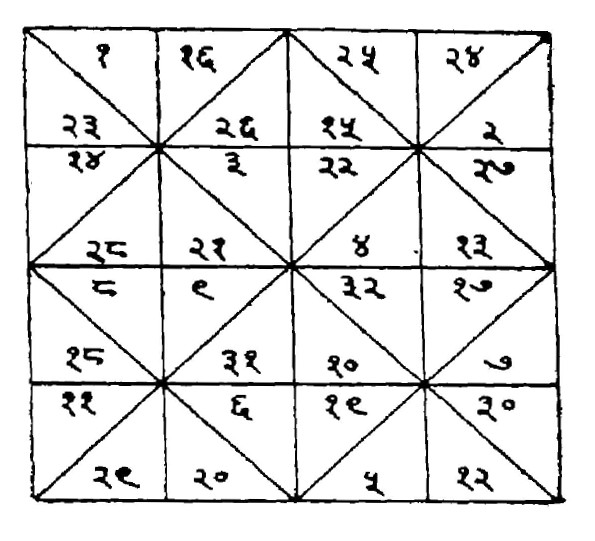
\includegraphics[scale=0.3]{graphics/413.jpg}
\end{figure}
\vspace{-2mm}

एतयोः फले १३२
\end{center}

\newpage

\begin{figure}[h!]
    \centering
    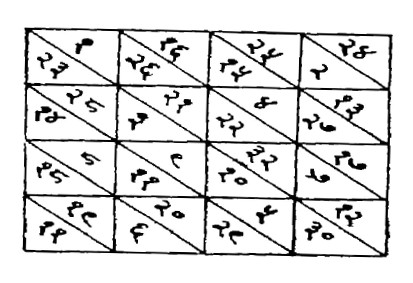
\includegraphics[scale=0.3]{graphics/414_1.jpg}
    
\end{figure}

\begin{figure}[h!]
    \centering
    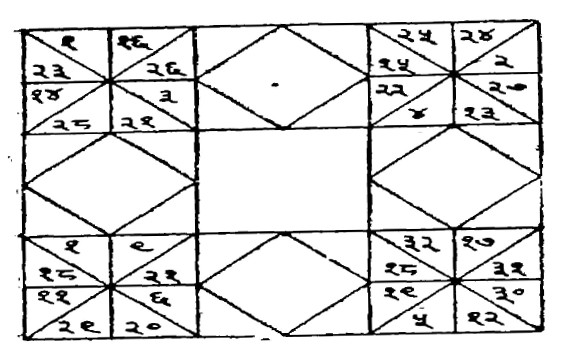
\includegraphics[scale=0.3]{graphics/414_2.jpg}
    
\end{figure}

\begin{figure}[h!]
    \centering
    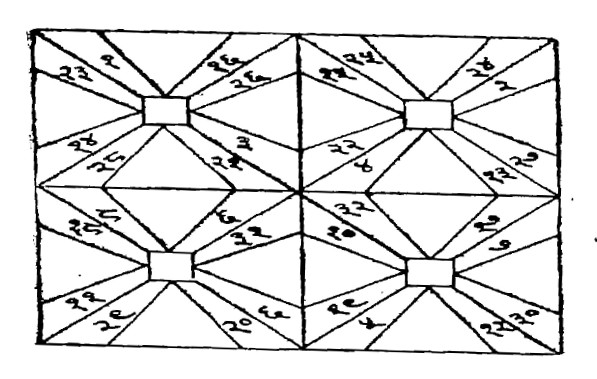
\includegraphics[scale=0.3]{graphics/414_3.jpg}
    
\end{figure}

\newpage

\textbf{सूत्रम्~।}

\begin{quote}
{\gk सर्वतो भद्रसञ्ज्ञस्य\\
तिर्यक्कोष्ठान् प्रपूरयेत्~।\\
वज्रं पङ्कजसञ्ज्ञस्य\\
मण्डपद्वयमत्र तु~॥~५०~॥	}
\end{quote}

(\,ऊर्ध्वानष्टाभवैरङ्कैस्तिर्यग्भिरथ पूर्ववत्\,)\\

\textbf{उदाहरणम्~।}

\begin{quote}
{\ex सर्वतोभद्रसञ्ज्ञं मे\\
चतुःषष्टिगृहं वद~।\\
वज्रपङ्कजसञ्ज्ञं च\\
कोष्ठैकाङ्कयुतौ समम्~॥~१४~॥	}
\end{quote}

अत्रैकक्रमजनितैकादिचयैरङ्कैर्जातादष्टभद्राद्यथोक्तकरणेन \;जातं \;सर्वतोभद्रं \;तद्दर्शनं यथा

\newpage

\begin{figure}[h!]
    \centering
    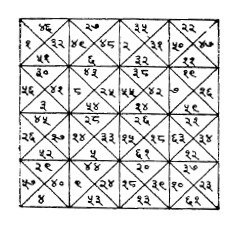
\includegraphics[scale=0.65]{graphics/416_1.jpg}
    
\end{figure}
\vspace{-8mm}

\begin{center}
भद्रफलम् २६०~।\\
\vspace{6mm}

तथैव मण्डपाज्जातम् भद्रफलम् २६०~।
\end{center}
\vspace{-4mm}

\begin{figure}[h!]
    \centering
    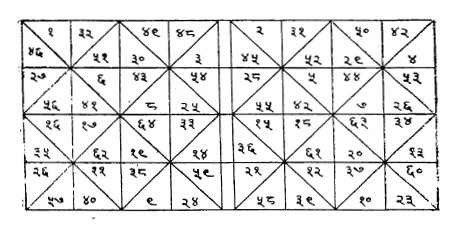
\includegraphics[scale=0.5]{graphics/416_2.jpg}
    
\end{figure}

एवमत्राष्टाष्टकोष्ठाङ्कसंयोगः समः स्यात्~। तस्मादेवाष्टभद्राच्चतुष्किकाभद्रम्~। सर्वफलम् १३०~।

\newpage

\begin{figure}[h!]
    \centering
    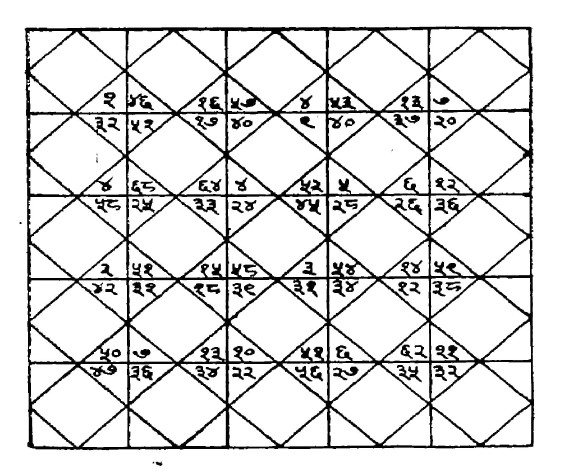
\includegraphics[scale=0.4]{graphics/417.jpg}
    
\end{figure}

\textbf{सूत्रम्~।}

\begin{quote}
{\gk सर्वतोभद्रविधिना\\
पृथक् भद्रत्रयोद्भवैः~।\\
अङ्कैः प्रपूरणं कार्यं\\
प्रतिभद्रं क्रमोत्क्रमात्~॥~५१~॥}	
\end{quote}

\textbf{उदाहरणम्~।}

\begin{quote}
{\ex द्वादशकोष्ठस्थानाम्\\
अङ्कानां संयुतिः समा भवति~।\\
कथयार्य गणितगर्वं\\
प्रवहसि यदि ते द्रुतं गणक~॥~१५~॥}
\end{quote}

\newpage

अत्र चतुर्भद्रत्रयाज्जातमायतभद्रदर्शनम्~।

\begin{table}[h]
\setlength{\extrarowheight}{2pt} \setlength{\tabcolsep}{2pt}	
\centering
\hspace{4mm} \begin{tabular}{|c|c|c|c|}
	\hline
	१ & २४ & ३७ & ३६\\
	\hline
	४२ & ३१ & ६ & १६\\
	\hline
	४०& ३० & ७ & १८\\
	\hline
\end{tabular} \hspace{2mm} 
\begin{tabular}{|c|c|c|c|}
	\hline
	२ & २३ & ३८ & ३५\\
	\hline
	४१ & ३२ & ५ & २०\\
	\hline
	४४ & २९ & ८ & १७\\
	\hline
\end{tabular} \hspace{2mm} 
\begin{tabular}{|c|c|c|c|}
	\hline
	३ & २२ & ३९ & ३४\\
	\hline
	४० & ३३ & ४ & २१\\
	\hline
	४५ & २८ & ९ & १९\\
	\hline
\end{tabular}
\end{table}
\vspace{-4mm}

\begin{center}
	द्वादशकोष्ठाङ्कफलम् २९४~।	
\end{center}
\vspace{-8mm}

\begin{figure}[h!]
    \centering
    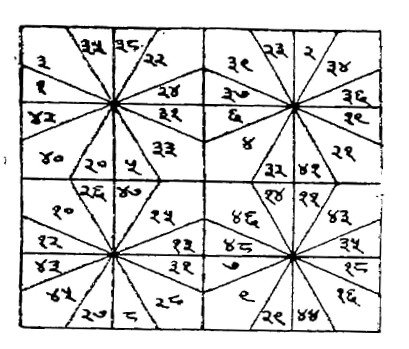
\includegraphics[scale=0.4]{graphics/418.jpg}
    
\end{figure}
\vspace{-6mm}

\begin{table}[h]
\setlength{\extrarowheight}{1pt} \setlength{\tabcolsep}{1pt}	
\centering
\begin{tabular}{|c|c|c|c|c|c|c|c|c|c|c|c|}
	\hline
& 	१ &  &  & १६ & & & ४&  & & १३ &  \\
	\hline
२७ &  & ४६ & १७ &  & ५७ & ९ & & ५३ & ३७ & & ७\\
	\hline
&५१ &  &  & ४१ & & &  ४० &  & & २० & \\ 
	\hline
& ४ & & &  ६४ & & & ५२ & & &६ & \\
\hline
५८ & & ६८ & ३३ & &४ & ४५ & & ५ & २६ & &१२\\
\hline
& २५ & & & २४ & &  &  २८ & & & ३६ & \\
\hline
&  २ & & &  १५ &  &  &  ३ & & & १४ & \\
\hline
४२ & & ५१ & १८ & & ५८ & ३१ & & ५४ & १२ & & ५९ \\
\hline 
& ३२ & & & ३९ & & & ४३ & & &३८& \\
\hline
& ५० & & & १३ & & & ५१ & & & ६२ & \\
\hline
४७ & & ७ & २४ & & १० & ५६ & & ६ & ३५ & & ११\\
\hline
& २६ & & & २३ & &  & २७ & &  & ३२ & \\
\hline 
\end{tabular}
\end{table}

\newpage

\begin{table}[h]
\setlength{\extrarowheight}{2pt} \setlength{\tabcolsep}{2pt}	
\centering
\begin{tabular}{|c|c|c|c|c|c|c|c|c|c|c|c|c|c|}
	\hline
१ & ४६ & ~~ & ~~ & १६ & ५७ & ~~ & ~~ & ४ & ५३ & ~~ & ~~ & १३ & ७\\
\hline
३२ & ५१ &  &  & १७ & ४० & ~~ &  &९ & ४० & ~~ & ~~ &३७ & २०\\
\hline
&  & ~~ & ~~ & ~~ & ~~ & ~~ & ~~ & ~~ & ~~ &  & ~~ & ~~ & \\
\hline
&  & ~~ & ~~ & ~~ & ~~ & ~~ & ~~ & ~~ & ~~ &  & ~~ & ~~ & \\
\hline
४ & ६८ & ~~ & ~~ & ६४ & ४ & ~~ & ~~ &५२ & ५ &  & ~~ & ६ & १२ \\
\hline
५८ & २५ & ~~ & ~~ & ३३ & २४ & ~~ & ~~ & ४५ & २८ & ~~ & ~~ & २६ & ३६ \\ 
\hline
&  & ~~ & ~~ & ~~ & ~~ & ~~ & ~~ & ~~ & ~~ &  & ~~ & ~~ & \\
\hline
&  & ~~ & ~~ & ~~ & ~~ & ~~ & ~~ & ~~ & ~~ &  & ~~ & ~~ & \\
\hline
२ & ५१ & ~~ & ~~ & १५ & ५८ & ~~ & ~~ & ३ & ५४ & ~~ & ~~ &१४ & ५९\\
\hline
४२ & ३१ & ~~ & ~~ &१८ & ३९ & ~~ & ~~ & ३१ & ४३ & ~~ & ~~ & १२ & ३८ \\
\hline
&  & ~~ & ~~ & ~~ & ~~ & ~~ & ~~ & ~~ & ~~ &  & ~~ & ~~ & \\
\hline
&  & ~~ & ~~ & ~~ & ~~ & ~~ & ~~ & ~~ & ~~ &  & ~~ & ~~ & \\
\hline
५० & ७ & ~~ & ~~ &१३ & १० & ~~ & ~~ &५१ & ६ & ~~ & ~~ & ६२ & ११\\
\hline
४७ & २६ & ~~ & ~~ & ३४ & २३ & ~~ & ~~ & ५७ & २७ & ~~ & ~~ &३५ & ३२\\
\hline
\end{tabular}
\end{table}

\vspace{-3mm}
\begin{center}
सर्वस्वस्तिकानि भद्राणि च समाप्तानि~।	
\end{center}
\vspace{2mm}

\textbf{अथ विविधं सूत्रम्~।}

\begin{quote}
{\gk चतुर्भद्रैस्त्रिभिः प्राग्वत्\\
आयतं कल्पयेत् ततः~।\\
तत्कर्णसंस्थितैरङ्कैः\\
दलपङ्क्तिं प्रपूरयेत्~॥~५२~॥\\
एककोणान्तरेणास्मिन्\\
अङ्कानां पूरणक्रिया~।}
\end{quote}

\newpage

\begin{quote}
{\gk षडस्त्राभ्यन्तरस्थानां\\
दलानामङ्कसंयुतिः~॥~५३~॥\\
द्वादशानां फलं पद्म-\\
भद्रं सञ्जायते ध्रुवम्~।}
\end{quote}

\textbf{उदाहरणम्~।}

\begin{quote}
{\ex एकाद्येकचयैस्त्रिषोडशमितैः\\
	पद्मस्थिताङ्कैः कथं\\
	भद्रं षट्कजसञ्ज्ञकं द्रुततरं\\
	ब्रूह्याशु मे चायतात्~।\\
	षट्कोणोदरवर्तिभानुदलगा-\\
	ङ्कैक्ये समं किं फलं\\
	वृत्तान्तर्दलसंयुतिर्भवति वा\\
	तुल्या कथं स्यात् सखे~॥~१६~॥}
\end{quote}

अत्र चतुर्भद्रत्रयाज्जातमायतफलम्\textendash

\begin{table}[h]
\setlength{\extrarowheight}{2pt} \setlength{\tabcolsep}{2pt}	
\centering
\hspace{6mm} \begin{tabular}{|c|c|c|c|}
\hline
१ & २४ & ३७ & ३६\\
\hline
४२ & ३१ & ६ & १९\\
\hline
१२ & १३ & ४८ &  २५\\
\hline
४३ & ३० & ७ & १८\\
\hline
\end{tabular} \hspace{2mm} 
\begin{tabular}{|c|c|c|c|}
\hline
२ & २३ & ३८ & ३५\\
\hline
४१ & ३२ & ५ & २०\\
\hline
११ & १४ & ४७ &  २६\\
\hline
४१ & २९ & ८ & १७\\
\hline
\end{tabular} \hspace{2mm}
\begin{tabular}{|c|c|c|c|}
	\hline
	३ & २२ & ३९ & ३४\\
	\hline
	४० & ३३ & ४ & २१\\
	\hline
	१० & १५ & ४६ &  २७\\
	\hline
	४५ & २८ & ९ & १६\\
	\hline
\end{tabular}

\end{table}

\newpage

एकादिस्थानजनितानां भद्राणामायताङ्कैरापूर्य जाते पद्मवृत्तषडस्रभद्रे~। पद्मवृत्तषडस्रयोः फले २९४।२८४~।

\begin{figure}[h!]
    \centering
    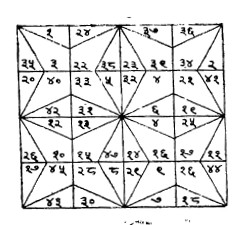
\includegraphics[scale=0.7]{graphics/421_1.jpg}
\end{figure}
\vspace{-4mm}

\begin{figure}[h!]
    \centering
    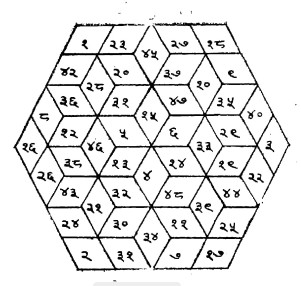
\includegraphics[scale=0.7]{graphics/421_2.jpg}
    
\end{figure}

\newpage

\begin{figure}[h!]
    \centering
    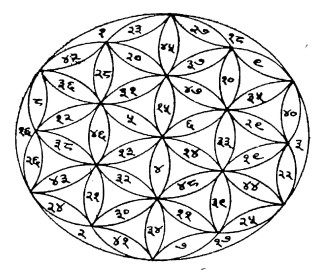
\includegraphics[scale=0.65]{graphics/422.jpg}
    
\end{figure}

एवं नानाप्रकारेण समुद्भवन्ति~।\\

\textbf{अथ समायते सूत्रम्~।}

\begin{quote}
{\gk त्रिचतुःपञ्चषडाद्यैः\\
भद्रे त्र्यस्रादिकानि भद्राणि~।\\
स्युर्वर्तुलानि तत्र च\\
फलरहितफलं हि तद्धृदयम्~॥~५४~॥}
\end{quote}

आयतभद्रेण तथा द्विविधं भद्रं भवत्येव~।

\newpage

\textbf{उदाहरणम्~।}

\begin{quote}
{\ex त्र्यस्रादीनां चतुर्णां पृथगपि गगना-\\
भ्राब्धितुल्यं फलं स्यात्~।\\
भद्रे त्र्यस्रादिकेभ्यः कथय मम किमा-\\
कारभूतानि तानि~॥\\
भद्राणि द्विप्रभेदं खरसगुणफलं\\
चायतात् यत् प्रयातम्~।\\
भद्रं भद्रज्ञ, चेत् सुप्रकटगणितज-\\
ज्ञानगर्वावृतोऽसि~॥~१७~॥}
\end{quote}

त्र्यस्रादीनां \,वृत्तानां \,समफलम् \,४०० \,इष्टानि \,द्वित्रिभद्राणि \,तेषां \,कल्पितावाद्युत्तरौ त्रिभद्रे आ १ उ ५, चतुर्भद्रे ३९।९, २६०।३३३ एभिः पृथक् पृथक् जनितमेतत् ४०० जातानि क्रमेण हृदयानि १७५।९४~। १४०।६७ त्रिभद्रस्य न्यासः

\begin{center}
\begin{tabular}{|c|c|c|}
	\hline
	६० & ४५ & १२०\\
	\hline	
	१३५ & ७५ & १५\\
	\hline
	३०१ & ०५ & ८०\\
	\hline
\end{tabular}
\end{center}

\newpage

\begin{center}
त्रिभद्रवृतिदर्शनम्	
\end{center}

\begin{figure}[h!]
    \centering
    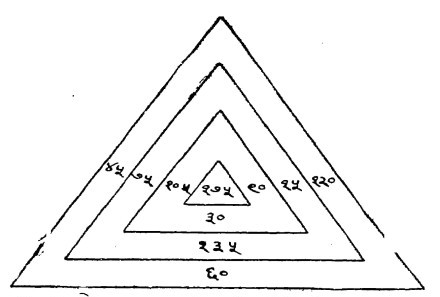
\includegraphics[scale=0.5]{graphics/424_1.jpg}
    
\end{figure}

\begin{figure}[h!]
    \centering
    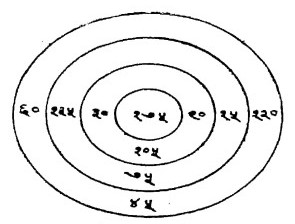
\includegraphics[scale=0.5]{graphics/424_2.jpg}
    
\end{figure}

\newpage

आयतभद्रस्य फलम् ३६०~। एकाद्येकोत्तरेण जातमष्टभद्रम्~।

\begin{table}[h]
	\centering
\begin{tabular}{|c|c|c|c|}
	\hline
	१& १६ & २५ & २४\\
	\hline	
	२८ & २१ & ४ & १३\\
	\hline
	८ & ९ & ३२  & १७\\
	\hline
	२९ & २० & ५ & १२\\
	\hline
\end{tabular} \hspace{4mm} 
\begin{tabular}{|c|c|c|c|}
	\hline
	२& १५ & २६ & २३\\
	\hline	
	२० & २२ & ३ & १४\\
	\hline
	७ & १० & ३०  & १८\\
	\hline
	३० & १९ & ६ & ११\\
	\hline
\end{tabular}

\end{table}

\begin{center}
आयतभद्रदर्शनम्~।
\end{center}
\vspace{-6mm}

\begin{figure}[h!]
    \centering
    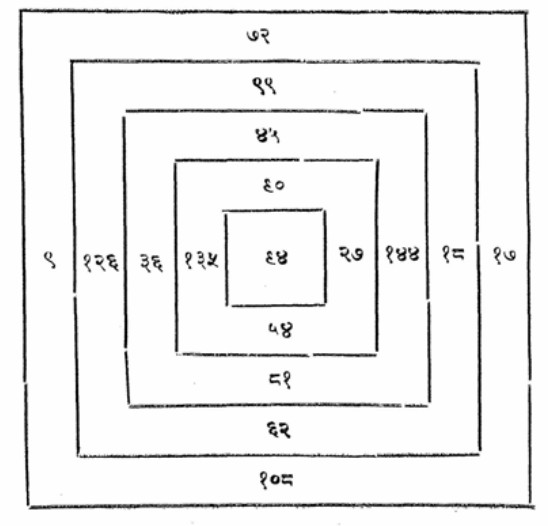
\includegraphics[scale=0.4]{graphics/425.jpg}
    
\end{figure}

\newpage

\begin{figure}[h!]
    \centering
    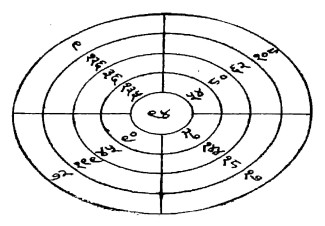
\includegraphics[scale=0.6]{graphics/426_1.jpg}
    
\end{figure}

\begin{center}
पञ्चभद्राज्जातं पञ्चास्त्रं वृत्तम्~।
\end{center}
\vspace{-6mm}

\begin{figure}[h!]
    \centering
    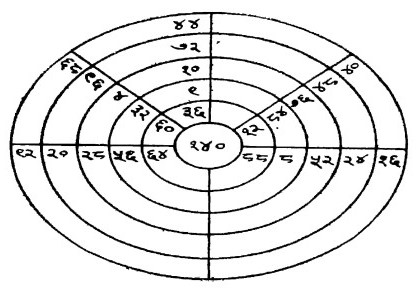
\includegraphics[scale=0.6]{graphics/426_2.jpg}
    
\end{figure}

\newpage

\begin{figure}[h!]
    \centering
    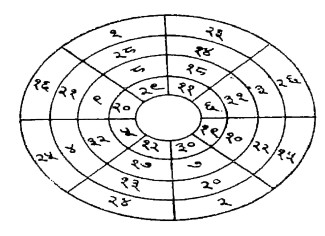
\includegraphics[scale=0.6]{graphics/427_1.jpg}
    
\end{figure}

\begin{figure}[h!]
    \centering
    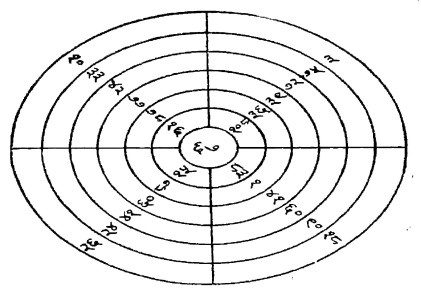
\includegraphics[scale=0.6]{graphics/427_2.jpg}
    
\end{figure}

\newpage

\begin{quote}
	
{\gk सङ्क्षेपतो गणितजाड्यविनाशनानि\\
भद्राणि भद्रमतिदानि समीरितानि~।\\
नोक्तानि तानि घनवर्गपदात्मकानि\\
ग्रन्थप्रसारणभयात् बहुलक्रियाणि~॥~५५~॥\\}

\phantomsection \label{ch15}
{\gk आसीत् सौजन्यदुग्धाम्बुधिरवनिसुर-\\
श्रेणिमुख्यो जगत्यां\\
प्रख्यः श्रीकण्ठपादद्वयनिहितमनाः\\
शारदाया निवासः~।\\
श्रौतस्मार्तार्थवेत्ता सकलगुणनिधिः\\
शिल्पविद्याप्रगल्भः\\
शास्त्रे शस्त्रे च तर्के प्रचुरतरगतिः\\
श्रीनृसिंहो नृसिंहः~॥~१~॥}\\

{\gk तत्सूनुरस्ति गणितार्णवकर्णधारः\\
श्रीशारदाप्रचुरलब्धवरप्रसादः~।\\
नारायणः पृथुयशा गणितस्य पाटीं\\
श्रीकौमुदीमिति मुदे गुणिनां प्रचक्रे~॥~२~॥}
\end{quote}

\newpage

\begin{quote}
{\gk यावत् सप्तकुलाचलाः क्षितितले\\
यावच्चतुःसागरा\\
यावत् सूर्यमुखा ग्रहाश्च गगने\\
यावत् ध्रुवस्तारकाः~।\\
स्थेयात् तावदियं सदोदितवती\\
श्रीकौमुदी कौमुदी-\\
पूरस्वच्छयशःप्रवाहसुभगा\\
नारायणेन्दोः स्तुता~॥~३~॥\\}

{\gk नारायणाननसुधाकरमण्डलोत्थां\\
च तुर्यसूक्तिरचनामृतबिन्दुवृन्दाम्~।\\
प्रीत्यैव सज्जनचकोरगणाः पिबन्तु\\
श्रीकौमुदीमुदितहृत्कुमुदः सदैताम्~॥~४~॥\\}

{\gk गजनगरविमित\textendash \,१२७८\textendash \,शाके \\
दुर्मुखवर्षे च बाहुले मासि~।\\
धातृतिथौ कृष्णदले\\
गुरौ समाप्तिगतं गणितम्~॥~५~॥}
\end{quote}

\newpage

\begin{center}
\textbf{इति श्रीसकलकलानिधिश्रीमन्नृसिंहनन्दनगणितविद्याचतुरानननारायणपण्डितविरचितायां गणितपाट्यां कौमुद्याख्यायां भद्रगणितं नाम चतुर्दशो व्यवहारः~।}\\
\vspace{10mm}

\textbf{समाप्तेयं गणितकौमुदी~।}\\
\vspace{4mm}

\rule{2cm}{0.4mm}
\end{center}


\end{document}
